\documentclass[9pt]{extarticle}
% \documentclass[9pt,twocolumn]{extarticle}

\usepackage[utf8]{inputenc}    % For UTF-8 character encoding
\usepackage[T1]{fontenc}       % For proper font encoding
\usepackage{lmodern}           % Improved font rendering
\usepackage{amsmath}   % For advanced mathematical formatting
\usepackage{amssymb}   % For mathematical symbols
% \usepackage{geometry}  % Adjust page margins
\usepackage{enumerate} % For custom lists
\usepackage{xcolor}  % for coloring
\usepackage{amsthm}
\usepackage{pdfpages}
\usepackage{graphicx}

\newtheorem{theorem}{Theorem}[section]
\newtheorem{invariant}{Invariant}
\newtheorem{lemma}[theorem]{Lemma}
\newtheorem{corollary}[theorem]{Corollary}
\newtheorem{definition}[theorem]{Definition}
\usepackage{listings}  % for code listings
\usepackage{tikz-cd}
\usepackage{tikz}
\usetikzlibrary{trees}

\usepackage{forest}
\usepackage{titlesec}
% \titlespacing*{\section}{0pt}{6pt plus 2pt minus 2pt}{1pt}
% \titlespacing*{\subsection}{0pt}{4pt plus 1pt minus 1pt}{1pt}
\titlespacing*{\subsubsection}{0pt}{3pt plus 1pt minus 1pt}{1pt}
\usetikzlibrary{arrows.meta}
\usetikzlibrary{arrows.meta,decorations.pathreplacing,calc}
\lstset{frame=tb,
  language=C,
  aboveskip=3mm,
  belowskip=3mm,
  showstringspaces=false,   
  columns=flexible,
  basicstyle={\small\ttfamily},
  numbers=none,
  numberstyle=\tiny\color{gray},
  keywordstyle=\color{blue},
  commentstyle=\color{brown},
  stringstyle=\color{orange},
  breaklines=true,
  breakatwhitespace=true,
  tabsize=3
}
\usepackage{dsfont}
\renewcommand{\baselinestretch}{0.5}

\linespread{0.9}
\usepackage[twoside,
            left=0.8in,         % inner margin
            right=0.8in,        % outer margin
            top=0.8in,
            bottom=0.8in,
            bindingoffset=1cm % extra space near binding
           ]{geometry}
% \geometry{top=0.4in, bottom=0.6in, left=0.4in, right=1.6in}
% \geometry{top=0.3in, bottom=0.2in, left=0.2in, right=0.2in}
\setlength{\columnseprule}{0.4pt}
\begin{document}


\title{CS3230}
\author{@Wxy2003-xy}
\date{}
\maketitle

\newpage
\tableofcontents
\newpage

\section{Asymptotic Analysis}
\begin{align*}
    &O(g): \{f: \exists c > 0 \land n_0 > 0, \forall n \geq n_0, 0 \leq f(n) \leq c \cdot g(n)\} \\
    &\Omega(g): \{f: \exists c > 0 \land n_0 > 0, \forall n \geq n_0, 0 \leq c \cdot g(n) \leq f(n)\} \\
    &\Theta(g): \{f: \exists c_1, c_2 > 0 \land n_0 > 0, \forall n \geq n_0, c_1 \cdot g(n) \leq f(n) \leq c_2 \cdot g(n)\} \\
    %
    &o(g): \{f: \forall c > 0, \exists n_0 > 0, \forall n \geq n_0, 0 \leq f(n) < c \cdot g(n)\} \\ 
    &\omega(g): \{f: \forall c > 0, \forall n \leq n_0, 0 \leq c \cdot g(n) < f(n)\} \\
\end{align*}
\subsection{Proof with limit}

\section*{Limit-Based Proofs for Asymptotic Notation}
\textit{Hint.} Work with eventually-positive functions and ratios. Let $f,g:\mathbb{N}\to\mathbb{R}$ (or $\mathbb{R}_{>0}\to\mathbb{R}$) with $g(n)\neq 0$ for all large $n$. Write $R(n)=\frac{|f(n)|}{|g(n)|}$ unless otherwise noted.

\subsection*{Definitions (epsilon/constant form)}
\begin{align*}
f(n)\in O(g(n)) &\iff \exists\,C>0,\,N:\ \forall n\ge N,\ |f(n)|\le C\,|g(n)|.\\
f(n)\in \Omega(g(n)) &\iff \exists\,c>0,\,N:\ \forall n\ge N,\ |f(n)|\ge c\,|g(n)|.\\
f(n)\in \Theta(g(n)) &\iff f\in O(g)\ \text{and}\ f\in \Omega(g).\\
f(n)\in o(g(n)) &\iff \forall \varepsilon>0\ \exists\,N:\ \forall n\ge N,\ |f(n)|\le \varepsilon |g(n)|.\\
f(n)\in \omega(g(n)) &\iff \forall M>0\ \exists\,N:\ \forall n\ge N,\ |f(n)|\ge M |g(n)|.\\
f(n)\sim g(n) &\iff \lim_{n\to\infty}\frac{f(n)}{g(n)}=1\quad\text{(asymptotic equivalence).}
\end{align*}

\subsection*{Limit criteria (what to prove with limits)}
Assume $g(n)>0$ eventually.
\begin{itemize}
  \item \textbf{Little-$o$:}\quad $f\in o(g)\iff \displaystyle\lim_{n\to\infty}\frac{f(n)}{g(n)}=0$.
  \item \textbf{Little-$\omega$:}\quad $f\in \omega(g)\iff \displaystyle\lim_{n\to\infty}\frac{f(n)}{g(n)}=\infty$ (equivalently $\liminf R(n)=\infty$).
  \item \textbf{Big-$\Theta$:}\quad $f\in \Theta(g)$ if and only if
  \[
    0<\liminf_{n\to\infty}\frac{|f(n)|}{|g(n)|}\ \le\ \limsup_{n\to\infty}\frac{|f(n)|}{|g(n)|}\ <\infty.
  \]
  In particular, if $\lim \frac{f}{g}=c\in(0,\infty)$ then $f\in\Theta(g)$.
  \item \textbf{Big-$O$:}\quad A \emph{sufficient and necessary} condition:
  \[
    f\in O(g)\iff \limsup_{n\to\infty}\frac{|f(n)|}{|g(n)|}<\infty.
  \]
  In particular, if $\lim \frac{f}{g}=c\in[0,\infty)$ then $f\in O(g)$.
  \item \textbf{Big-$\Omega$:}\quad A \emph{sufficient and necessary} condition (for eventually positive $f$):
  \[
    f\in \Omega(g)\iff \liminf_{n\to\infty}\frac{|f(n)|}{|g(n)|}>0.
  \]
  In particular, if $\lim \frac{f}{g}=c\in(0,\infty]$ then $f\in \Omega(g)$.
  \item \textbf{Asymptotic equivalence ($\sim$):} $f\sim g\ \Rightarrow\ f\in\Theta(g)$ (take $c=1$ above). Converse is false in general.
\end{itemize}

\subsection*{Proof templates}
\paragraph{To show $f\in o(g)$:} Compute $L=\lim \frac{f}{g}$. If $L=0$, write: 
\[
\text{Given }\varepsilon>0,\ \exists N:\ \forall n\ge N,\ \frac{|f(n)|}{|g(n)|}<\varepsilon.
\]

\paragraph{To show $f\in O(g)$:} Show $\limsup R(n)=M<\infty$, then choose $C>M+1$ and $N$ s.t. $R(n)\le C$ for all $n\ge N$.

\paragraph{To show $f\in \Omega(g)$:} Show $\liminf R(n)=m>0$, then pick $c=m/2$ and $N$ s.t. $R(n)\ge c$ for all $n\ge N$.

\paragraph{To show $f\in \Theta(g)$:} Either (i) show $\lim \frac{f}{g}=c\in(0,\infty)$, or (ii) give both $O$ and $\Omega$ bounds via limsup/liminf.

\paragraph{To show $f\in \omega(g)$:} Show $\lim \frac{f}{g}=\infty$ (or $\liminf R(n)=\infty$). Then for any $M>0$, pick $N$ with $R(n)\ge M$ for all $n\ge N$.

\subsection*{examples (limit proofs)}
\begin{itemize}
  \item $n^\alpha \in o(n^\beta)$ for $0\le \alpha<\beta$:\ \ $\lim \frac{n^\alpha}{n^\beta}=\lim n^{\alpha-\beta}=0$.
  \item $\log^k n \in o(n^\varepsilon)$ for any fixed $k,\varepsilon>0$:\ \ use $\lim \frac{\log^k n}{n^\varepsilon}=0$ (e.g.\ L'Hôpital or known hierarchy).
  \item $a^n \in \omega(n^k)$ for $a>1$:\ \ $\lim \frac{a^n}{n^k}=\infty$.
  \item $(n+\sin n)\in \Theta(n)$:\ \ $\lim \frac{n+\sin n}{n}=1$ by squeeze.
  \item $n^p(\log n)^q \in \Theta(n^p \log^q n)$:\ \ trivial $c=1$.
\end{itemize}

\subsection*{Notes}
\begin{itemize}
  \item Using ratio limits when $g(n)$ changes sign or is zero infinitely often. Fix by restricting to $n$ large where $g(n)>0$.
  \item Concluding $\Theta$ from $\lim \frac{f}{g}=0$ or $\infty$ (those give $o$ or $\omega$, not $\Theta$).
  \item Forgetting absolute values in oscillatory cases (e.g.\ $(-1)^n n$); prefer limsup/liminf or bound with envelopes.
  \item Assuming $O$ implies a limit exists—false. $f(n)=\sin n$ is $O(1)$ but the ratio to $1$ has no limit.
\end{itemize}

\subsection*{Handy equivalences}
\[
f\in o(g)\ \Longleftrightarrow\ g\in \omega(f),\qquad
f\in O(g)\ \Longleftrightarrow\ g\in \Omega(f).
\]
If $f\sim g$ then $f-g=o(g)$ (and $o(f)$), and $f\in\Theta(g)$.

\[\Theta(f) = O(f) \cap \Omega(f)\]
\begin{proof}
    1. prove: $O(f) \cap \Omega(f) \subseteq \Theta(f) $\\  
    From definition: \\
    \begin{align*}
        &\Theta(f(n)): \{g: \exists c_1, c_2 > 0, \exists n_0 \geq 0, \forall n \geq n_0, c_1 \cdot f(n) \leq g(n) \leq c_2 \cdot f(n)\}\\
        &O(f(n)) \cap \Omega(f(n)): \{g: \exists c_1 > 0, \exists n_1 \geq 0, \forall n \geq n_1, 0 \leq g(n) \leq c_1 \cdot f(n)\\ &\land 
        \exists c_2 > 0, \exists n_2 \geq 0, \forall n \geq n_2, 0 \leq c_2 \cdot f(n) \leq g(n)\}
    \end{align*}
    When $0 \leq c_1 \leq c_2, O(f(n)) \cap \Omega(f(n)): 
    \{g: \exists n_1, n_2 \geq 0, \forall n \geq \{\max(n_1, n_2)\}, 0 \leq c_1 f(n) \leq g(n) \leq c_2 f(n)\}$\\
    $\implies $ $O(f) \cap \Omega(f) \subseteq \Theta(f) $\\  
    2. prove: $\Theta(f) \subseteq O(f) \cap \Omega(f)$\\ 
    $(f(n) > 0 \land, c_1 \leq, c_2) \implies (0 \leq c_1 f(n) \leq g(n) \land 0 \leq g(n) \leq c_2 f(n))$\\ 
    $\implies $  $\Theta(f) \subseteq O(f) \cap \Omega(f)$\\ 
    $\implies $  $\Theta(f) = O(f) \cap \Omega(f)$\\ 


\end{proof}
\[\lim_{n \rightarrow \infty} \frac{f(n)}{g(n)} = 0 \implies f(n) \in o(g(n))\]
\begin{proof}
    From lmit definition, $\forall \epsilon > 0, \exists n_0 \geq 0, 
    \forall n \geq n_0, \frac{f(n)}{g(n)} < \epsilon$. Let $c = \epsilon, 
    \frac{f(n)}{g(n)} < \epsilon, f(n) < c \cdot g(n)$. $f(n) \geq 0, f(n) \in o(g(n))$
\end{proof}
\[\lim_{n \rightarrow \infty} \frac{f(n)}{g(n)} = \infty \implies f(n) \in \omega(g(n))\]
\begin{proof}
    From $\lim_{n \rightarrow \infty} \frac{f(n)}{g(n)} = \infty \iff \lim_{n \rightarrow \infty} \frac{g(n)}{f(n)} = 0$, as \\
    $\lim_{x \rightarrow \infty} \frac{1}{f(x)} = \frac{1}{\lim_{x\to\infty} f(x)}, \lim_{n \rightarrow \infty} \frac{g(n)}{f(n)} = \frac{1}{\lim_{n \rightarrow \infty}\frac{f(n)}{g(n)}} = \frac{1}{\infty} = 0$.\\
    Similarly, $\forall \epsilon > 0, \exists n_0 \geq 0, 
    \forall n \geq n_0, \frac{g(n)}{f(n)} < \epsilon$. Let $c = \frac{1}{\epsilon}, 
    \frac{g(n)}{f(n)} < \epsilon, c \cdot g(n) < f(n)$.\\
\end{proof}
\[0 < \lim_{n \rightarrow \infty} \frac{f(n)}{g(n)} < \infty \implies f(n) \in \Theta(g(n))\]
\begin{proof}
    Definitions:\\
    $\Theta(g): \{f: \exists c_1, c_2 > 0 \land n_0 > 0, \forall n \geq n_0, c_1 \cdot g(n) \leq f(n) \leq c_2 \cdot g(n)\}$\\
    $O(g): \{f: \exists c > 0 \land n_0 > 0, \forall n \geq n_0, 0 \leq f(n) \leq c \cdot g(n)\}$ \\
    $o(g): \{f: \forall c > 0, \exists n_0 > 0, \forall n \geq n_0, 0 \leq f(n) < c \cdot g(n)\}$\\
    Prove: $\Theta(f) = O(f) \setminus o(f)$
    \begin{proof}
        1. $\Theta(f) \subseteq O(f) \setminus o(f)$\\
            Suppose $g(n) \in \Theta(f), \Theta(f) = O(f) \cap \Omega(f) \implies g(n) \in O(f)$. \\
            Suppose $g(n) \in o(f), (\exists c_1, c_2 > 0, \exists n_1 > 0, \forall n \geq n_1, 0 \leq c_1 \cdot f(n) \leq g(n) \leq c_2 \cdot f(n)) \land (\forall c_3 > 0, \exists n_2 > 0, \forall n \geq n_2, 0 \leq g(n) < c_3 \cdot f(n))$\\
            Let $c_3 < c_1, c_1 \cdot f(n) \leq g(n) < c_3 \cdot f(n)$, contradiction, \\
            $\implies g(n) \in \Theta(f) \rightarrow g(n) \notin o(f)$\\
            $\implies \Theta(f) \subseteq O(f) \setminus o(f)$\\
        2. \[O(f) \setminus o(f) \subseteq \Theta(f) = \]
            \[
            \begin{aligned}
            \{g:\ & (\exists c_1 > 0, \exists n_1 > 0, \forall n \geq n_1,\ 0 \leq g(n) \leq c_1 \cdot f(n)) \\
                & \land\ \neg(\forall c_2 > 0, \exists n_2 > 0, \forall n \geq n_2,\ 0 \leq g(n) < c_2 \cdot f(n)) \} \\
            \{g:\ & (\exists c_1 > 0, \exists n_1 > 0, \forall n \geq n_1,\ 0 \leq g(n) \leq c_1 \cdot f(n)) \\
                & \land\ (\exists c_2 > 0, \forall n_2 > 0, \exists n \geq n_2,\ (g(n) < 0 \lor g(n) \geq c_2 \cdot f(n))) \} \\
            \{g:\ & \exists c_1 > c_2 > 0, \forall n_2 > 0, \exists n_1 \geq n_2, \forall n \geq n_1,\ 0 \leq c_2 \cdot f(n) \leq g(n) \leq c_1 \cdot f(n) \} \\[0.5em]
            \{g:\ & \exists c_1 > c_2 > 0, \exists n_0 > 0, \forall n \geq n_0,\ 0 \leq c_2 \cdot f(n) \leq g(n) \leq c_1 \cdot f(n) \}
            \end{aligned}
            \]
    \end{proof}
\end{proof}

\subsection{Reflexivity}
\subsubsection{$f(n)\in O(f(n))$}
\begin{proof}
    Suppose $f(n) > 0$\\
    Let $c = 1, n_0 = 1, \forall n \geq n_0, 0 \leq f(n) \leq f(n), \implies f(n) \in O(f(n))$
\end{proof}
\subsubsection{$f(n) \in \Omega(f(n))$, $f(n) \in \Theta(f(n))$}
Similarly, by picking the right $c$ and $n_0$ it's easy to prove existential statements.

\subsection{Transitivity}
\subsubsection{$f(n) \in O(g(n)) \land g(n) \in O(h(n)) \implies f(n) \in O(h(n))$}
\begin{proof}
    \begin{align*}
        &\exists c_1 > 0, n_1 > 0, \forall n \geq n_1, 0 \leq f(n) \leq c_1 \cdot g(n)\\
        &\exists c_2 > 0, n_2 > 0, \forall n \geq n_2, 0 \leq g(n) \leq c_2 \cdot h(n)
    \end{align*}
    Let $c_1 = 1, n_0 = \max(n_1, n_2)$, $0 \leq f(n) \leq g(n) \leq c_2 \cdot h(n) \implies \exists c_2 > 0, \forall n \geq n_0, 0 \leq f(n) \leq c_2 \cdot h(n)$\\
    $\implies f(n) \in O(h(n))$  
\end{proof}
\subsubsection{$f(n) \in \Omega(g(n)) \land g(n) \in \Omega(h(n)) \implies f(n) \in \Omega(h(n))$}
Similar to $O(f(n))$ proof
\subsubsection{$f(n) \in \Theta(g(n)) \land g(n) \in \Theta(h(n)) \implies f(n) \in \Theta(h(n))$}
\begin{align*}
    &\exists c_1^{[1]}, c_2^{[1]}> 0, n_1 > 0, \forall n \geq n_1, 0 \leq c_1^{[1]} \cdot g(n) \leq f(n) \leq c_2^{[1]} \cdot g(n)\\
    &\exists c_1^{[2]}, c_2^{[2]} > 0, n_2 > 0, \forall n \geq n_2, 0 \leq c_1^{[2]} \cdot h(n) \leq g(n) \leq c_2^{[2]} \cdot h(n)
\end{align*}
Let $c_1^{[1]} = c_2^{[1]} = 1, f(n) = g(n), $\\
$0 \leq c_1^{[2]} \cdot h(n) \leq f(n) \leq c_2^{[2]} \cdot h(n) \implies f(n) \in \Theta(h(n))$
\subsubsection{$f(n) \in o(g(n)) \land g(n) \in o(h(n)) \implies f(n) \in o(h(n))$}
\begin{proof}
    \begin{align}
        &\forall c_1 > 0, \exists n_1 > 0, \forall n \geq n_1, 0 \leq f(n) < c_1 \cdot g(n)\\
        &\forall c_2 > 0, \exists n_2 > 0, \forall n \geq n_2, 0 \leq g(n) < c_2 \cdot h(n)
    \end{align}
From  (2), $\forall c_2 > 0, \exists n_2 > 0, \forall n \geq n_2, 0 \leq c_1 \cdot g(n) < c_1 \cdot c_2 \cdot h(n)$
    \begin{align*}
        &\forall c_1, c_2 > 0, \exists n_1, n_2 > 0, \forall n \geq \max(n_1, n_2), 0 \leq f(n) < c_1 \cdot g(n) < c_1 \cdot c_2 \cdot h(n)
    \end{align*}
    \[\forall c_1, c_2 > 0, \exists n_1, n_2 > 0, \forall n \geq \max(n_1, n_2), 0 \leq f(n) < c_1 \cdot c_2 \cdot h(n)\]
\end{proof}

\subsubsection{$f(n) \in \omega(g(n) \land g(n) \in \omega(h(n))) \implies f(n) \in \omega(h(n))$}
    \begin{align*}
        &\forall c_1 > 0, \exists n_1 > 0, \forall n \geq n_1, 0 \leq c_1 \cdot g(n) < f(n)\\
        &\forall c_2 > 0, \exists n_2 > 0, \forall n \geq n_2, 0 \leq c_2 \cdot h(n) < g(n)
    \end{align*}
    \[\forall c_1, c_2 > 0, \exists n_1, n_2 > 0, \geq \max(n_1, n_2), 0 \leq c_1 \cdot c_2 \cdot h(n) < c_1 \cdot g(n) < f(n)\]
\subsection{Symmetry: $f(n) \in \Theta(g(n)) \iff g(n)\in \Theta(f(n))$}
\begin{proof}
    \begin{align*}
        & f(n) \in \Theta(g(n)) \implies\\
        &\exists c_1, c_2> 0, n_1 > 0, \forall n \geq n_1, 0 \leq c_1 \cdot g(n) \leq f(n) \leq c_2 \cdot g(n) \implies\\
        & \left(0 \leq g(n) \leq \frac{1}{c_1}\cdot f(n) \leq \frac{c_2}{c_1}\cdot g(n)\right) \land \left( 0 \leq \frac{c_1}{c_2} \cdot g(n) \leq \frac{1}{c_2} \cdot f(n) \leq g(n)\right) \implies \\
        & 0 \leq \frac{1}{c_2} \cdot f(n) \leq g(n) \leq \frac{1}{c_1}\cdot f(n)\\
    \end{align*}
    Identical proof for the other direction
\end{proof}
\subsection{Complementary}
\subsubsection{$f(n) \in O(g(n) \iff g(n) \in \Omega(f(n)))$}
\begin{proof}
    \begin{align*}
        & f(n) \in O(g(n)) \implies \\
        & \exists c > 0 \land n_0 > 0, \forall n \geq n_0, 0 \leq f(n) \leq c \cdot g(n) \implies \\
        & 0 \leq \frac{1}{c}\cdot f(n) \leq g(n)
    \end{align*}
Proof for the other direction and the next statement are identical.
\end{proof}
\subsubsection{$f(n) \in o(g(n) \iff g(n) \in \omega(f(n)))$}

\subsection{Problems}
\subsubsection*{$3^{n + 1} \in O(3^n)$}
\begin{proof}
    \begin{align*}
        & 3^{n+ 1} = 3 \cdot 3^n\\
        & let c = 4, n_0 = 1, \forall n \geq n_0, \\
        & 3^{n+1} < c\cdot 3^n
    \end{align*}
\end{proof}
\subsubsection*{$4^n \notin O(2^n)$}
\begin{proof}
    Suppose $f(n) = 4^n \in O(2^n)$,\\
    \begin{align*}
        & \exists c > 0, n_0 > 0, \forall n \geq n_0, 0 \leq 2^{2 \times n} \leq c\cdot 2^n \implies\\
        & 0 \leq 2^n \leq c\\
        & 0 \leq n \leq \log_2c (const)\\
        & \text{n is upper bounded by a constant, a contradiction}
    \end{align*}
\end{proof}
\subsubsection*{$2^{\lfloor \log_2n \rfloor} \in \Theta(n)$}
\begin{proof}
    \begin{align*}
        & \text{Let } k = \lfloor \log_2 n\rfloor, 2^k \leq n < 2^{k+1} = 2 \cdot 2^k\\
        & \text{Let } c_1 = \frac{1}{2}, c_2 = 1, n_0 = 2, \\
        & \frac{n}{2} < 2^k \leq n
    \end{align*}
\end{proof}

\subsubsection*{For constant $i$, $a > 0$, $(n + a)^i \in O(n^i)$}
\begin{proof}
    \begin{align*}
        & \forall a > 0, \exists n_0 > a, \forall n \geq n_0, f(n) = (n + a)^i \leq (2n)^i = 2^i \cdot n^i, \\
        &\text{Let } c = 2^i, n_0 = a + 1, \forall n \geq n_0, 0 \leq f(n) \leq c \cdot n^i
    \end{align*}
\end{proof}
\subsubsection*{Prove: $2^{\log_2n} \in O(n)$}
\begin{proof}
    Let $c = 2, n_0 = 2, \forall n \geq n_0, 2^{\log_2n} = n \implies 0 \leq n \leq 2n$
\end{proof}
\subsubsection*{Prove: $2^{\log_2n} \in \Omega(n)$}
\begin{proof}
    Let $c = 0.5, n_0 = 2, \forall n \geq n_0, 2^{\log_2n} = n \implies 0 \leq 0.5n \leq n$
\end{proof}
\subsubsection*{Prove: $2^{\log_2n} \notin \Theta(\sqrt{n})$}
\begin{proof}
    Suppose otherwise, $\exists c_1, c_2 > 0, n_0 > 0, \forall n \geq n_0, 0 \leq c_1 \cdot \sqrt{n} \leq n \leq c_2 \sqrt{n}$,\\
    \begin{align*}
        & c_1 \leq \sqrt{n} \leq c_2\\
        & \text{However, } \lim_{n \rightarrow \infty} \sqrt{n}= \infty, \text{ thus cannot be bound by constant } c_2, \text{a contradiction.}
    \end{align*}
\end{proof}
\subsubsection*{Prove: $2^{\log_2n} \notin \omega(n)$}
\begin{proof}
    Suppose otherwise, $\forall c > 0, \exists n_0 > 0, \forall n \geq n_0, 0 \leq c\cdot n < n$. When $c = 2, \forall n_0 > 0, \forall n \geq n_0, 2n \geq n$, a contradiction.
\end{proof}

\subsubsection*{Rank order of growth}
\subsubsection*{$f_1(n) = \log n$}
By reflexivity, 
\[f_1(n) \in \Theta(\log n)\]
\subsubsection*{$f_2(n) = n!$}
By reflexivity, 
\[f_2(n) \in \Theta(n!)\]
\subsubsection*{$f_3(n) = 2^n + n$}
\[f_3(n) \in \Theta(2^n)\]
\begin{proof}
    
\end{proof}
\subsubsection*{$f_4(n) = n^{2.3} + 16n$}
\[f_4(n) \in \Theta(n^{2.3})\]
\begin{proof}
    
\end{proof}
\subsubsection*{$f_5(n) = \log(n^{2})$}
\[f_5(n) \in \Theta(\log(n))\]
\begin{proof}
    Assume base 2, $f_5(n) = \log(n^2) = 2\log(n)$, let $c_1 = 1, c_2 = 3, n_0 = 2, \\ \forall n \geq n_0, 0 \leq \log(n) \leq \log(n) \leq 3\log(n)$
\end{proof}
\[\Theta(\log(n)) \subseteq o(n^{2.3}) \subseteq o(2^n) \subseteq o(n!)\]
\begin{proof}
    \begin{align*}
        & \lim_{n \rightarrow \infty} \frac{\log(n)}{n^{2.3}} = \lim_{n \rightarrow \infty} \frac{(\log(n))'}{(n^{2.3})'} = \lim_{n \rightarrow \infty} \frac{1}{\ln(2)n^{1.3}} = 0, \\
        & \implies \forall f(n) \in \Theta(\log(n)), f(n) \in o(n)\\
    \end{align*}

    \begin{align*}
        & \lim_{n \rightarrow \infty} \frac{n^{2.3}}{2^n} = \lim_{n \rightarrow \infty} \frac{2.3\ln(n)}{n\cdot \ln(2)} = \lim_{n \rightarrow \infty} \frac{2.3}{n\cdot \ln(2)} = 0, \\
        & \implies \forall f(n) \in \Theta(n^{2.3}), f(n) \in o(2^n)
    \end{align*}

    \begin{align*}
        & \lim_{n \rightarrow \infty} \frac{2^n}{n!} = \lim_{n \rightarrow \infty} \frac{\prod_{r=1}^{n}2}{\prod_{r=1}^{n} r} = 0,  \forall n > 2\\
        & \implies \forall f(n) \in \Theta(2^n), f(n) \in o(n!)
    \end{align*}

\end{proof}
\subsection{Math utils}
\[a^{\log_bn} = n^{\log_ba}\]
\[\log_ab = \frac{\log_cb}{\log_ca}\]
\subsection*{Close form formulae for $\sum_{i=1}^{n}i^k$}
\begin{align*}
    \sum_{i=1}^n i   &= \frac{n(n+1)}{2}, \\[6pt]
    \sum_{i=1}^n i^2 &= \frac{n(n+1)(2n+1)}{6}, \\[6pt]
    \sum_{i=1}^n i^3 &= \left(\frac{n(n+1)}{2}\right)^2, \\[6pt]
    \sum_{i=1}^n i^4 &= \frac{n(n+1)(2n+1)(3n^2+3n-1)}{30}, \\[6pt]
    \sum_{i=1}^n i^5 &= \frac{n^2 (n+1)^2 (2n^2+2n-1)}{12}.
\end{align*}
\[\sum_{i=1}^{n} i^p = \frac{1}{p+1}\sum_{j=0}^{p} (-1)^j \binom{p+1}{j}\, B_j \, n^{p+1-j},
\quad p\in\mathbb{N}\] 
where \(B_j\) are the Bernoulli numbers.    \text{(https://en.wikipedia.org/wiki/Faulhaber)}
\subsubsection*{Example}
\begin{align*}
    \sum_{i=1}^{k} i^8 &= \frac{1}{9}\sum_{j=0}^{8} (-1)^j \binom{9}{j}\, B_j\\
    &= \frac{1}{9}(\binom{9}{0}(1)k^9 - \binom{9}{1}(\frac{1}{2})k^8 + ... + \binom{9}{8}(\frac{-1}{30}k))
\end{align*}
\[h(k) = \sum_{i=1}^{k}i^8 \in O(k^9)\]
\begin{table}[h!]\centering
    \renewcommand{\arraystretch}{1.1}
    \setlength{\tabcolsep}{6pt}
    \begin{tabular}{r l r l r l r l}
    $n$ & $B_n$ & $n$ & $B_n$ & $n$ & $B_n$ & $n$ & $B_n$ \\\hline
    0  & $1$              & 5  & $0$                   & 10 & $\tfrac{5}{66}$        & 15 & $0$ \\
    1  & $-\tfrac{1}{2}$  & 6  & $\tfrac{1}{42}$       & 11 & $0$                    & 16 & $-\tfrac{3617}{510}$ \\
    2  & $\tfrac{1}{6}$   & 7  & $0$                   & 12 & $-\tfrac{691}{2730}$   & 17 & $0$ \\
    3  & $0$              & 8  & $-\tfrac{1}{30}$      & 13 & $0$                    & 18 & $\tfrac{43867}{798}$ \\
    4  & $-\tfrac{1}{30}$ & 9  & $0$                   & 14 & $\tfrac{7}{6}$         & 19 & $0$ \\
    \hline
    \end{tabular}
    \caption{First 20 Bernoulli numbers $B_n$}
    \end{table}
    
\subsection{Techniques}
Log trick: 
\[\log(\prod_{i=1}^{n} f(x)) = \sum_{i=1}^{n} \log(f(x))\]
Harmonic series
\begin{align*}
    H_n&= \sum_{i=1}^{n}\frac{1}{i} = \ln(n) + \gamma + \Theta(\frac{1}{n})\\
    H^{(p)}_n &= \sum_{i=1}^{n}\frac{1}{i^p}\quad \text{converges}\\
\end{align*}
\begin{table}[h!]\centering
    \renewcommand{\arraystretch}{1.1}
    \setlength{\tabcolsep}{6pt}
    \begin{tabular}{r l r l r l r l}
    $n$ & $\gamma_n$ & $n$ & $\gamma_n$ & $n$ & $\gamma_n$ & $n$ & $\gamma_n$ \\\hline
    1  & $1.000000$ & 6  & $0.658251$ & 11 & $0.257651$ & 16 & $0.254040$ \\
    2  & $0.806853$ & 7  & $0.647998$ & 12 & $0.256744$ & 17 & $0.253542$ \\
    3  & $0.734722$ & 8  & $0.640544$ & 13 & $0.255939$ & 18 & $0.253095$ \\
    4  & $0.697123$ & 9  & $0.634774$ & 14 & $0.255228$ & 19 & $0.252691$ \\
    5  & $0.673343$ & 10 & $0.630331$ & 15 & $0.254599$ & 20 & $0.252322$ \\
    \hline
    \end{tabular}
    \caption{First 20 approximations $\gamma_n = H_n - \ln n$ to the Euler--Mascheroni constant}
    \end{table}
    
For example, for recurrence $T(n) = T(n-1) + \frac{1}{n}$, $T(n) \in \Theta(\log(n))$. If the recurrence have terms like
$\frac{n}{(\log(n))^p}$, it usually connects to $H_n^{(p)}$ where $T\rightarrow ... \rightarrow S(m) = S(m-1) + \frac{1}{m}$\\
Sterling formula:\\
\( n! \sim \sqrt{2\pi n}\,\left(\frac{n}{e}\right)^n \)\\
\newpage
\section{Recurrence}
\subsection{master theorem}
\begin{theorem}[Master Method]
Consider the recurrence
\[
T(n) = aT\!\left(\tfrac{n}{b}\right) + f(n),
\]
where $a, b$ are constants. Then:
\begin{itemize}
    \item[(A)] If $f(n) = O(n^{\log_b a - \varepsilon})$ for some constant $\varepsilon > 0$, then
    \[
    T(n) = O(n^{\log_b a}).
    \]

    \item[(B)] If $f(n) = \Theta(n^{\log_b a})$, then
    \[
    T(n) = \Theta(n^{\log_b a} \log n).
    \]

    \item[(C)] If $f(n) = \Omega(n^{\log_b a + \varepsilon})$ for some constant $\varepsilon > 0$, and if $f$ satisfies the smoothness condition
    \[
    af(n/b) \leq c f(n) \quad \text{for some constant } c < 1,
    \]
    then
    \[
    T(n) = \Theta(f(n)).
    \]
\end{itemize}
\end{theorem}
% Drop this into your doc; no extra packages required.
% Legend: p = log_b a.  We write n^{\log_b a} symbolically for clarity.
\subsubsection{Common recurrence table}
\begin{center}
    \scriptsize
    \setlength{\tabcolsep}{4pt}
    \renewcommand{\arraystretch}{1.15}
    \begin{tabular}{ccccccccc}
    \hline
    $a$ & $b$ & $p=\log_b a$ & $n^{-1}$ & $\log n$ & $n$ & $n\log n$ & $n^{2}$ & $n^{3}$ \\
    \hline
    1 & 2 & 0 & $\Theta(1)$ & $\Theta(\log^{2} n)$ & $\Theta(n)$ & $\Theta(n\log n)$ & $\Theta(n^{2})$ & $\Theta(n^{3})$ \\
    2 & 2 & 1 & $\Theta(n)$ & $\Theta(n)$ & $\Theta(n\log n)$ & $\Theta(n\log^{2} n)$ & $\Theta(n^{2})$ & $\Theta(n^{3})$ \\
    3 & 2 & $\log_{2}3$ & $\Theta(n^{\log_{2}3})$ & $\Theta(n^{\log_{2}3})$ & $\Theta(n^{\log_{2}3})$ & $\Theta(n^{\log_{2}3})$ & $\Theta(n^{2})$ & $\Theta(n^{3})$ \\
    4 & 2 & 2 & $\Theta(n^{2})$ & $\Theta(n^{2})$ & $\Theta(n^{2})$ & $\Theta(n^{2})$ & $\Theta(n^{2}\log n)$ & $\Theta(n^{3})$ \\
    \hline
    1 & 3 & 0 & $\Theta(1)$ & $\Theta(\log^{2} n)$ & $\Theta(n)$ & $\Theta(n\log n)$ & $\Theta(n^{2})$ & $\Theta(n^{3})$ \\
    2 & 3 & $\log_{3}2$ & $\Theta(n^{\log_{3}2})$ & $\Theta(n^{\log_{3}2})$ & $\Theta(n)$ & $\Theta(n\log n)$ & $\Theta(n^{2})$ & $\Theta(n^{3})$ \\
    3 & 3 & 1 & $\Theta(n)$ & $\Theta(n)$ & $\Theta(n\log n)$ & $\Theta(n\log^{2} n)$ & $\Theta(n^{2})$ & $\Theta(n^{3})$ \\
    4 & 3 & $\log_{3}4$ & $\Theta(n^{\log_{3}4})$ & $\Theta(n^{\log_{3}4})$ & $\Theta(n^{\log_{3}4})$ & $\Theta(n^{\log_{3}4})$ & $\Theta(n^{2})$ & $\Theta(n^{3})$ \\
    \hline
    1 & 4 & 0 & $\Theta(1)$ & $\Theta(\log^{2} n)$ & $\Theta(n)$ & $\Theta(n\log n)$ & $\Theta(n^{2})$ & $\Theta(n^{3})$\\
    2 & 4 & $\tfrac12$ & $\Theta(n^{\log_{4}2})$ & $\Theta(n^{\log_{4}2})$ & $\Theta(n)$ & $\Theta(n\log n)$ & $\Theta(n^{2})$ & $\Theta(n^{3})$ \\
    3 & 4 & $\log_{4}3$ & $\Theta(n^{\log_{4}3})$ & $\Theta(n^{\log_{4}3})$ & $\Theta(n)$ & $\Theta(n\log n)$ & $\Theta(n^{2})$ & $\Theta(n^{3})$ \\
    4 & 4 & 1 & $\Theta(n)$ & $\Theta(n)$ & $\Theta(n\log n)$ & $\Theta(n\log^{2} n)$ & $\Theta(n^{2})$ & $\Theta(n^{3})$ \\
    \hline
    \end{tabular}
    \end{center}
    

    \subsection*{Master Theorem: Worked Examples (3 Cases)}
    \textit{Hint.} Let \(p=\log_b a\). Compare \(f(n)\) to \(n^p\):\\
    \(\quad\)Case 1: \(f(n)=O(n^{p-\varepsilon}) \Rightarrow T(n)=\Theta(n^p)\).\\
    \(\quad\)Case 2: \(f(n)=\Theta(n^p\log^k n) \Rightarrow T(n)=\Theta(n^p\log^{k+1}n)\).\\
    \(\quad\)Case 3: \(f(n)=\Omega(n^{p+\varepsilon})\) and \(a\,f(n/b)\le c\,f(n)\) for some \(c<1 \Rightarrow T(n)=\Theta(f(n))\).
    
    \paragraph{Case 1: subpolynomially smaller than \(n^p\).}
    \begin{itemize}
      \item \textbf{1A.} \(T(n)=4T(n/2)+n\). Here \(a=4,b=2\Rightarrow p=\log_2 4=2\). Since \(f(n)=n=O(n^{2-\varepsilon})\) (take \(\varepsilon=1\)), \(\boxed{T(n)=\Theta(n^2)}\).
      \item \textbf{1B.} \(T(n)=2T(n/2)+\sqrt{n}\). \(p=\log_2 2=1\). \(f(n)=n^{1/2}=O(n^{1-\varepsilon})\) with \(\varepsilon=1/2\). \(\boxed{T(n)=\Theta(n)}\).
      \item \textbf{1C.} \(T(n)=8T(n/4)+n\log n\). \(p=\log_4 8=\tfrac{3}{2}\). Since \(\log n=O(n^{0.25})\), \(n\log n=O(n^{1.5-0.25})\). \(\boxed{T(n)=\Theta(n^{3/2})}\).
    \end{itemize}
    
    \paragraph{Case 2: same polynomial order (polylog factor).}
    \begin{itemize}
      \item \textbf{2A.} \(T(n)=2T(n/2)+n\) (mergesort). \(p=1\), \(f(n)=n=\Theta(n^p)\) (\(k=0\)). \(\boxed{T(n)=\Theta(n\log n)}\).
      \item \textbf{2B.} \(T(n)=9T(n/3)+n^2\). \(p=\log_3 9=2\), \(f(n)=n^2=\Theta(n^p)\) (\(k=0\)). \(\boxed{T(n)=\Theta(n^2\log n)}\).
      \item \textbf{2C.} \(T(n)=4T(n/2)+n^2\log^3 n\). \(p=2\), \(f(n)=n^2\log^3 n=\Theta(n^p\log^3 n)\). \(\boxed{T(n)=\Theta(n^2\log^4 n)}\).
    \end{itemize}
    
    \paragraph{Case 3: polynomially larger than \(n^p\) (with regularity).}
    \begin{itemize}
      \item \textbf{3A.} \(T(n)=2T(n/2)+n^2\). \(p=1\). \(f(n)=n^2=\Omega(n^{1+\varepsilon})\) with \(\varepsilon=1\). Regularity: \(2\cdot(n/2)^2=n^2/2\le c n^2\) for \(c=\tfrac12<1\). \(\boxed{T(n)=\Theta(n^2)}\).
      \item \textbf{3B.} \(T(n)=3T(n/2)+n^2\). \(p=\log_2 3\approx1.585\). \(f(n)=n^2=\Omega(n^{p+\varepsilon})\) with \(\varepsilon\approx0.415\). Regularity: \(3\cdot(n/2)^2=\tfrac34 n^2\) (\(c=0.75<1\)). \(\boxed{T(n)=\Theta(n^2)}\).
      \item \textbf{3C.} \(T(n)=4T(n/2)+n^3\). \(p=2\). \(f(n)=n^3=\Omega(n^{2+1})\). Regularity: \(4\cdot(n/2)^3=\tfrac12 n^3\) (\(c=0.5<1\)). \(\boxed{T(n)=\Theta(n^3)}\).
    \end{itemize}
    
    \noindent\textit{Borderline note.} When \(f(n)=n^p/\log n\) or similar, the vanilla Master Theorem does not apply directly; use extended forms (e.g., Akra--Bazzi).
    



\subsection{Telescoping}
For recurrence relation 
\[T: \mathbb{N} \rightarrow \mathbb{R},T(n) = a\cdot T(\frac{n}{b}) + f(n)\]
\begin{enumerate}
    \item Define operator $N_k: (N_kT)(n) = \frac{T(n)}{n^k}$, where $k = \log_ba$
    \item Transform $T(n) \rightarrow R(n) := \frac{T(n)}{n^k}$
    \item Obtain the recurrence relation of $R(n) = R(\frac{n}{b}) + \frac{f(n)}{n^k}$
    \item Define map $E_b: \mathbb{Z} \rightarrow \mathbb{N}, E_b(m) = b^m$
    \item Define operator $P_b: (P_b H)(m) = H(E_b(m)) = H(b^m)$
    \item Transform $R(n) \rightarrow S(m) := P_b(R) = R \circ E_b, S(m) = R(b^m)$
\end{enumerate} 
    $
\begin{tikzcd}[row sep=small, column sep = tiny]
T(n) \arrow[r, "N_k"] \arrow[d, "n \mapsto n/b"] &[1em] R(n) \arrow[r, "P_b"] \arrow[d,"n \mapsto n/b"]&[1em] S(m) \arrow[d, "m \mapsto m-1"]\\
a\cdot T(\frac{n}{b}) + f(n) \arrow[r, <->] & R(\frac{n}{b}) + \frac{f(n)}{n^k} \arrow[r, <->]& S(m - 1) + \frac{f(b^m)}{b^{m\cdot k}} \\
\end{tikzcd}$\\
$T(n) = n^kR(n)\in \Theta(n^k H(n))\leftarrow R(n) \in \Theta(G(\log_bn)) = H(n) \\\leftarrow S(m) \in \Theta(S(0) + \sum_{i=1}^{m}\frac{f(b^i)}{b^{i\cdot k}}) = G(m)$

\[T(n) \sim n^{\log_ba} \sum_{i=1}^{\lfloor \log_b n\rfloor}\frac{f(b^i)}{b^{i\log_b a}}\]

% GPT version: 
% \subsection*{Telescoping}
% Assume $a>0$, integer $b\ge 2$, and $n$ ranges over powers of $b$ (or replace $n/b$ by $\lfloor n/b\rfloor$). For
% \[
% T:\mathbb{N}\to\mathbb{R},\qquad T(n)=a\,T\!\left(\frac{n}{b}\right)+f(n),
% \]
% \begin{enumerate}
%   \item Define $N_k$ by $(N_k T)(n):=\dfrac{T(n)}{n^{k}}$ with $k:=\log_b a$.
%   \item Let $R(n):=(N_k T)(n)=\dfrac{T(n)}{n^k}$.
%   \item Then $R$ satisfies
%   \[
%   R(n)=R\!\left(\frac{n}{b}\right)+\frac{f(n)}{n^k}\quad\text{since }a=b^k.
%   \]
%   \item Define $E_b:\mathbb{Z}_{\ge 0}\to\mathbb{N}$ by $E_b(m)=b^m$.
%   \item Define $P_b$ (precomposition) by $(P_b H)(m):=H(E_b(m))=H(b^m)$.
%   \item Let $S(m):=(P_b R)(m)=R\circ E_b(m)=R(b^m)$.
% \end{enumerate}

% \[
% \begin{tikzcd}[scale=1.2, transform shape, column sep=large, row sep=large]
% T(n) \arrow[r, "N_k"] \arrow[d, "n \mapsto n/b"'] &
% R(n) \arrow[r, "P_b"] \arrow[d, "n \mapsto n/b"'] &
% S(m) \arrow[d, "m \mapsto m-1"'] \\
% a\,T(n/b)+f(n) \arrow[r, "="] &
% R(n/b)+\dfrac{f(n)}{n^k} \arrow[r, "="] &
% S(m-1)+\dfrac{f(b^m)}{b^{mk}}
% \end{tikzcd}
% \]

% From the rightmost recurrence,
% \[
% S(m)=S(0)+\sum_{i=1}^{m}\frac{f(b^{i})}{b^{ik}},\qquad
% R(n)=S(\log_b n),\qquad
% T(n)=n^{k}\,R(n).
% \]

\subsubsection{Normalization: $T(n) = T(n^{\frac{1}{c}})$}
\[T(n) = AT(\sqrt{n}) + B \quad\text{include term } \log\log(n)\]
Consider recurrences of the form
\[
T(n) = n^{a} \, T\!\left(n^{1/c}\right) + f(n),
\]
where $a < 1$ and $c > 1$.  A useful technique is to normalize the
recurrence by dividing out the dominant power of $n$.

\paragraph{Step 1: Normalize.}
Define
\[
R(n) = \frac{T(n)}{n},
\]
so that
\[
R(n) = \frac{T(n)}{n}
= \frac{n^{a} \, T(n^{1/c})}{n} + \frac{f(n)}{n}
= n^{a-1} T(n^{1/c}) + \frac{f(n)}{n}
= \frac{T(n^{1/c})}{n^{1/c}} + \frac{f(n)}{n}
= R(n^{1/c}) + \frac{f(n)}{n}.
\]

For the special case $f(n) = n$, this simplifies to
\[
R(n) = R\!\left(n^{1/c}\right) + 1.
\]

\paragraph{Step 2: Change variables.}
Let $n = b^{m}$ (e.g.\ $b = c$), and define
\[
S(m) = R(b^{m}),
\]
which yields
\[
S(m) = S\!\left(\frac{m}{c}\right) + 1.
\]

\paragraph{Step 3: Linearize the recurrence.}
Let $m = c^{k}$ and define $U(k) = S(c^{k})$, giving the simple recurrence
\[
U(k) = U(k-1) + 1,
\]
whose solution is
\[
U(k) = \Theta(k).
\]

\paragraph{Step 4: Substitute back.}
Since $k = \Theta(\log m)$ and $m = \Theta(\log n)$, we obtain
\[
R(n) = \Theta(\log \log n),
\qquad
T(n) = n \cdot R(n) = \Theta\!\left(n \log \log n\right).
\]

This method cleanly converts non-standard recurrences of the form
$T(n^{1/c})$ into linear recurrences in $\log \log n$.\\
Examples:
\subsubsection*{Solving $T(n)=n^{2/3}T(n^{1/3})+n$ via Normalization}

We start with the recurrence
\[
T(n)=n^{2/3}T(n^{1/3})+n.
\]

\paragraph{Step 1: Normalize.}
Define
\[
R(n)=\frac{T(n)}{n}.
\]
Then
\[
R(n)
= \frac{T(n)}{n}
= \frac{n^{2/3}T(n^{1/3})}{n} + 1
= \frac{T(n^{1/3})}{n^{1/3}} + 1
= R(n^{1/3}) + 1.
\]
Thus the recurrence simplifies to
\[
R(n)=R(n^{1/3})+1.
\]

\paragraph{Step 2: Logarithmic substitution.}
Let
\[
n = 3^{m}, \qquad S(m)=R(3^{m}),
\]
so that
\[
S(m)=S\!\left(\frac{m}{3}\right)+1.
\]

\paragraph{Step 3: Linearize.}
Let
\[
m = 3^{k}, \qquad U(k)=S(3^{k}),
\]
giving the simple recurrence
\[
U(k)=U(k-1)+1.
\]
Hence \(U(k)=\Theta(k)\).

\paragraph{Step 4: Substitute back.}
Since
\[
k=\Theta(\log m),
\qquad
m=\Theta(\log n),
\]
we obtain
\[
R(n)=S(\log n)=\Theta(\log\log n).
\]
Finally,
\[
T(n) = n\,R(n)
= \Theta\!\left(n\log\log n\right).
\]

Thus the recurrence
\[
T(n)=n^{2/3}T(n^{1/3})+n
\]
has solution
\[
T(n)=\Theta\!\left(n\log\log n\right).
\]
\subsubsection{The Iterated Logarithm $\log^{*} n$}

The \emph{iterated logarithm} $\log^{*} n$ is defined as the number of
times the logarithm function must be applied before the value drops to~$1$ or
below.  Formally,
\[
\log^{*} n =
\begin{cases}
0, & n \le 1, \\[4pt]
1 + \log^{*}(\log n), & n > 1.
\end{cases}
\]
The base of the logarithm is not important for asymptotics; we typically
use base~$2$.

For example,
\[
\log^{*}(2^{65536}) = 5,
\]
since
\[
2^{65536} \xrightarrow{\log} 65536
\xrightarrow{\log} 16
\xrightarrow{\log} 4
\xrightarrow{\log} 2
\xrightarrow{\log} 1.
\]

The function $\log^{*} n$ grows extremely slowly---slower than
$\log\log\log n$---and remains below~$5$ for all practical values of~$n$.


\paragraph{Recurrences involving $\log^{*} n$.}
The iterated logarithm commonly appears in divide-and-reduce recurrences
where the input size decreases by repeated logarithms or exponentials.  
Typical examples include:
\begin{itemize}
    \item Recurrence of the form
    \[
        T(n) = T(\log n) + 1
        \quad\Longrightarrow\quad
        T(n) = \Theta(\log^{*} n).
    \]
    \item More generally,
    \[
        T(n) = T\!\left(n^{1/c}\right) + 1,
    \]
    when unrolled repeatedly, produces a sequence
    \(
        n, n^{1/c}, n^{1/c^{2}}, \dots
    \)
    whose length is $\Theta(\log^{*} n)$, hence
    \[
        T(n) = \Theta(\log^{*} n).
    \]
    \item Recurrences with decreasing exponentials,
    \[
        T(n) = T(\sqrt{n}) + 1,
    \]
    also yield
    \[
        T(n) = \Theta(\log^{*} n).
    \]
\end{itemize}

The function $\log^{*} n$ thus arises naturally in algorithms whose input
size shrinks by repeated logarithmic or root operations, such as union--find
with path compression or multi-level divide-and-conquer schemes.

\subsubsection{Comparison}
\[
\alpha(n) \;\ll\; \log^{*} n \;\ll\; \log\log n 
\;\ll\; (\log n)^k \;\ll\; n^{\varepsilon} \;\ll\; n \;\ll\; n^k 
\;\ll\; 2^n \;\ll\; n! \;\ll\; n^n \;\ll\; 2^{2^n}.
\]
\subsubsection*{more}
\[
1 \;\ll\; 
\alpha(n) \;\ll\; 
\log^{*} n \;\ll\; 
\log\log\log n \;\ll\; 
\log\log n \;\ll\; 
\log n \;\ll\; 
(\log n)^k \;\ll\; 
e^{(\log n)^{\alpha}} \ (0<\alpha<1) \;\ll\; 
n^{\varepsilon} \;\ll\; 
n \;\ll\; \]\[
n^k \;\ll\; 
n^{\log n} \;\ll\; 
2^{\sqrt{n}} \;\ll\; 
2^n \;\ll\; 
n! \;\ll\; 
n^n \;\ll\; 
2^{2^n}.
\]

\subsection*{Problems}
\subsection*{$T(n) = 4T(\frac{n}{4}) + \frac{n}{\log(n)}$}
Define $R(n) = \frac{T(n)}{n}$,
\begin{align*}
    R(n) &= \frac{4\cdot T(\frac{n}{4})}{n} + \frac{1}{\log(n)}\\
    &= R(\frac{n}{4}) + \frac{1}{\log(n)}
\end{align*}
Define $S(m) = R(4^n)$,
\begin{align*}
    S(m) & = S(m - 1) + \frac{\frac{4^m}{\log(4^m)}}{4^{m\cdot \log_4 4}}\\
    &= S(m - 1) + \frac{1}{m \log(4)}\\
    S(m) &\sim \frac{1}{\log(4)}\sum_{i=1}^{m} \frac{1}{i}\\
    S(m) &\in \Theta(\log m)\\
\end{align*}
Map back to $R(n)$ and $T(n)$, 
\begin{align*}
    S(m) \in \Theta(\log m) &\implies R(n) \in \Theta(\log(\log_4 n))\\
    &\implies T(n) \in n\log(\log(n))
\end{align*}


\subsection*{$T(n) = 4T(\frac{n}{2}) + \sqrt{n}$}
Define $R(n) = \frac{T(n)}{n^2}$,
\begin{align*}
    R(n) &= \frac{4\cdot T(\frac{n}{2})}{n^2} + \frac{\sqrt{n}}{n^2}\\
    &= R(\frac{n}{2}) + {n^{-\frac{3}{2}}}
\end{align*}
Define $S(m) = R(2^n)$,
\begin{align*}
    S(m) & = S(m - 1) + \frac{(2^m)^{-\frac{1}{2}}}{2^{m \cdot \log_2 4}}\\
    &= S(m - 1) + \frac{2^{-\frac{m}{2}}}{2^{2m}}\\
    &= S(m - 1) + \frac{1}{2^{\frac{3m}{2}}}\\
    S(m) &\sim \sum_{i=1}^{m} \frac{1}{2^{\frac{3i}{2}}} \text{ , clearly converges}\\
    S(m) &\in \Theta(1)\\
\end{align*}2
Maps back, 
\begin{align*}
    S(m) \in \Theta(1) &\implies R(n) \in \Theta(1)\\
    &\implies T(n) \in \Theta(n^2)
\end{align*}

\subsection*{$T(n) = T(\frac{n}{2}) + 2^{\sqrt{\log n}}$}
1. Using telescoping\\
$a = 0 \rightarrow \log_b a = 0, \text{there is no need for }T(n) \mapsto R(n).$\\
Define $S(m) = T(2^n)$, we have:\\
\begin{align*}
    S(m) &= S(m - 1) + 2^{\sqrt{\log{2^m}}}\\
    &= S(m - 1) + 2^{\sqrt{m}}    \\
    S(m) &\sim \sum_{i=1}^{m} 2^{\sqrt{i}} \approx \int_{1}^{m} 2^{\sqrt{x}} dx\\
\end{align*}
Solve for $ \int_{1}^{m} 2^{\sqrt{x}} dx$ by substitution: let $u = x^\frac{1}{2}$
\begin{align*}
    \frac{du}{dx} &= \frac{1}{2}x^{-\frac{1}{2}}\\
    dx &= \frac{1}{2u}\\
    \int 2^{\sqrt{x}} dx &= \int 2u\cdot 2^u du = 2\int u2^udu\\
    &= \frac{2^u(2u \ln(2) - 1)}{(\ln(2))^2} + C\\
    &= \frac{2^{\sqrt{x}}(2\sqrt{x} \ln(2) - 1)}{(\ln(2))^2} + C\\
    \int_{1}^{m} 2^{\sqrt{x}} dx &= \frac{1}{(\ln(2))^2}\left(2^{\sqrt{m}}(2\sqrt{m} \ln(2)-1)\right)
\end{align*}
Ignoring the constants, we have 
\begin{align*}
    S(m) &\sim \sum_{i=1}^{m} 2^{\sqrt{i}} \approx c\cdot 2^{\sqrt{m}}\sqrt{m}\\
    T(n) &\in \Theta(\sqrt{\log n}\cdot 2^{\sqrt{\log n}})
\end{align*}
\subsection*{Recurrence relation of merging $k$ arrays of size $n$}
\[T(k, n) = 2T(\frac{k}{2}, n) + \frac{nk}{2}\]
\[T(\frac{k}{2}, n) = 2T(\frac{k}{4}, n) + \frac{nk}{4}\]
Observed that the non-recursive funcion can be tightly bounded by $nk$,
\[T(k, n) = 2T(\frac{k}{2}, n) + cnk\]


With respect to $k$, Define $R(k, n) = \frac{T(k, n)}{k}$
\begin{align*}
    R(k, n) &= \frac{2 T(\frac{k}{2}, n)}{k} + cn\\
    &= R(\frac{k}{2}, n) + cn\\
\end{align*}
Define $S(m, n) = R(2^m, n)$,\\
$f(k, n) = cnk \rightarrow f(2^m, n) = cn2^m$, 
\begin{align*}
    S(m, n) &= S(m - 1, n) + \frac{cn2^m}{2^m}\\
    & \sim cn\sum_{i=1}^{m} 1\\
    S(m, n) &\in \Theta(nm)
\end{align*}
Maps back to $R(n)$,
\begin{align*}
    S(m, n) \in \Theta(n) &\implies R(k, n) \in \Theta(n\log(k))\\
    &\implies T(k, n) \in \Theta(nk\log(k))
\end{align*}

\subsection{WA1 Practice on Asymptotic analysis and recurrence}

\subsubsection*{Asymptotic Analysis}
\subsubsection{$f(n) = 3n + 1,\; g(n) = 4n$}
$f(n) \in \Theta(g(n))$
\begin{proof}
    $\Theta(g): \{f: \exists c_1, c_2 > 0 \land n_0 > 0, \forall n \geq n_0, c_1 \cdot g(n) \leq f(n) \leq c_2 \cdot g(n)\}$ \\

    Let $c_1 = \frac{3}{4}, c_2 = 1, n_0 = 1$, trivial
\end{proof}
\subsubsection{$f(n) = 3^n,\; g(n) = 2^n \cdot n^{10000}$}
$f(n) \in \omega(g(n))$
\begin{proof}
    $\lim_{n \rightarrow \infty} \frac{f(n)}{g(n)} = \lim_{n \rightarrow \infty}
     \frac{3^n}{2^n \cdot n^{10000}} = \lim_{n \rightarrow \infty} \frac{1.5^n}{n^{10000}} 
     = \lim_{n \rightarrow \infty} \frac{\ln(1.5)1.5^n}{10000n^{9999}}$\\
     $= ... = \lim_{n \rightarrow \infty} \frac{(\ln 1.5)^{10000}1.5^n}{10000!} = \infty \implies f(n) \in \omega(g(n))$
\end{proof}
\subsubsection{$f(n) = 2^n,\; g(n) = 2^{n+1}$}
$f(n) \in \Theta(g(n))$
\begin{proof}
    $g(n) = 2\cdot 2^n$, let $c_1 = \frac{1}{2}, c_2 = 1, n_0 = 2$, \\
    $\forall n \geq n_0, 1 \cdot 2^n \leq 2^n \leq 2\cdot 2^n \implies f(n) \in \Theta(g(n))$
\end{proof}
\subsubsection{$f(n) = 2^{(2^n)},\; g(n) = 2^{(2^{n+1})}$}
$f(n) \in o(g(n))$
\begin{proof}
    Let $u = 2^n$, $f(n) = 2^u, g(n) = 2^{2\cdot u}, g(n) = (f(n))^2. \forall n \in \mathbb{Z}^+, f(n) > 1$,\\
    $f(n) < (f(n))^2, 0 < f(n) < g(n) \implies f(n) \in o(g(n))$
\end{proof}
\subsubsection{$f(n) = \sum_{i=1}^n \frac{1}{2^i},\; g(n) = \sum_{i=1}^n \frac{i^{10000}}{2^i}$}
$f(n) \in \Theta(g(n))$
\begin{proof}
   $f(n) = \frac{\frac{1}{2}(\frac{1}{2^n} -1)}{\frac{1}{2} - 1} = 1 - \frac{1}{2^n}$, 
   trivial to show this is tightly upper bounded by constant. $f(n) \in \Theta(1)$\\
   Next we will show that the summation $g(n)$ converges. \\
   \[\lim_{n \rightarrow \infty} \frac{\frac{n^{10000}}{2^n}}{\frac{(n-1)^{10000}}{2^{n-1}}} 
   = \lim_{n \rightarrow \infty} \frac{n^{10000}}{2(n-1)^{10000}} = \lim_{n \rightarrow \infty} \frac{10000 n^{9999}}{20000(n-1)^{9999}} = \dots\]
   \[= \lim_{n \rightarrow \infty} \frac{10000!}{2(10000!)} = \frac{1}{2} < 1 \implies \sum_{i=1}^n \frac{i^{10000}}{2^i} \quad \text{converges}\]
   $g(n) \in \Theta(1) \implies h(n) \in \Theta(g(n)) \text{ by symmetry }\implies f(n) \in \Theta(g(n))$ by transitivity.
\end{proof}

\subsubsection{$f(n) = \log\log (n^n),\; g(n) = \log\log(2^{\sqrt{n}})$}
$f(n) \in \Theta(g(n))$
\begin{proof}
    $f(n) = \log(n \log(n )) = \log(n) + \log(\log(n))$\\
    $g(n) = \log(\sqrt{n}\log 2) = \log(\sqrt{n}) + \log(\log2) = \frac{1}{2}\log(n) + \log\log(2)$\\
    $L = \frac{f(n)}{g(n)} = \frac{\log n + \log(\log n)}{0.5 \log n + \log (\log 2)} = 
    \frac{1 + \frac{\log\log(n)}{\log(n)}}{\frac{1}{2} \frac{\log\log(2)}{\log(n)}}$\\
    $\lim_{n\rightarrow \infty} L = 2$\\
    $0 < \lim_{n \rightarrow \infty} \frac{f(n)}{g(n)} < \infty \implies f(n) \in \Theta(g(n))$
\end{proof}
\subsubsection{$f(n) = 2^{\sqrt{\log n}},\; g(n) = \sqrt{n}$}
$f(n) \in o(g(n))$
\begin{proof}
    $L = \frac{f(n)}{g(n)}, \log(L) = \log(f(n)) - \log(g(n)) = \sqrt{\log n}\log(2) - \frac{1}{2} \log(n) $\\
    $= -\frac{1}{2}\log n (1 - \frac{\log 2 \sqrt{\log n}}{\log n}) = -\frac{1}{2}\log n (1 - \frac{\log 2 }{\sqrt{\log n}}) $\\
    $\lim_{n\rightarrow\infty} \log(L) = -\infty \implies \lim_{n\rightarrow\infty} L = e^{-\infty} = 0^+ \implies f(n) \in o(g(n))$ 
\end{proof}

\subsubsection{$f(n) = 2^{\sqrt{\log n}},\; g(n) = 2^{2^{\sqrt{\log\log n}}}$}
$f(n) \in \omega(g(n))$
\begin{proof}
Let $u = \log\log n$, $f(u) = 2^{\sqrt{2^u}}, g(u) = 2^{\sqrt{u}}$\\
$L = \frac{f(u)}{g(u)} = \frac{2^{\sqrt{2^u}}}{2^{\sqrt{u}}}, \log(L) = \log(2) (\sqrt{2^u} - \sqrt{u}), \lim_{u \rightarrow \infty}\log(L) = \infty \implies
\lim_{u \rightarrow \infty}L = \infty$\\
$u = \log\log n $ is monotonous and unbounded, $\lim \frac{f(u)}{g(u)} = \infty \implies \lim \frac{f(n)}{g(n)} = \infty \implies f(n) \in \omega(g(n)) $
\end{proof}


\subsubsection{$f(n) = n^{\frac{1}{\log n}},\; g(n) = n^{\frac{1}{(\log n)^2}}$}
$f(n) \in \Theta(g(n))$
\begin{proof}
    Let $L = \frac{f(n)}{g(n)} = n^{\frac{1}{\log n} - \frac{1}{(\log n)^2}} = n^{\frac{\log n - 1}{(\log n)^2}}$\\
    $\log(L) = \log n (\frac{\log n - 1}{(\log n)^2}) = \frac{\log n - 1}{\log n} = 1 - \frac{1}{\log n}, $\\
    $\lim_{n \rightarrow \infty} \log(L) = 1 \implies \lim_{n \rightarrow \infty} L = 2 \implies f(n) \in \Theta(g(n))$
\end{proof}

\subsubsection{$f(n) = n^{\frac{1}{\log n}},\; g(n) = n^{\frac{1}{\sqrt{\log n}}}$}
$f(n) \in o(g(n))$
\begin{proof}
    Let $L = \frac{f(n)}{g(n)} = n^{\frac{1}{\log n} - \frac{1}{(\log n)^\frac{1}{2}}} = n^{\frac{1-(\log n)^{\frac{1}{2}}}{\log n}}$\\
    $\log(L) = \log n (\frac{1-\sqrt{\log n}}{\log n}) = 1-\sqrt{\log n} $\\
    $\lim_{n \rightarrow \infty} \log(L) = -\infty \implies \lim_{n \rightarrow \infty} L = 0^+ \implies f(n) \in o(g(n))$
\end{proof}

\subsection*{Recurrence}
Alternative method proof: \\
For recurrence relation 
\[T: \mathbb{N} \rightarrow \mathbb{R},T(n) = a\cdot T(\frac{n}{b}) + f(n)\]
\begin{enumerate}
    \item Define operator $N_k: (N_kT)(n) = \frac{T(n)}{n^k}$, where $k = \log_ba$
    \item Transform $T(n) \rightarrow R(n) := \frac{T(n)}{n^k}$
    \item Obtain the recurrence relation of $R(n) = R(\frac{n}{b}) + \frac{f(n)}{n^k}$
    \item Define map $E_b: \mathbb{Z} \rightarrow \mathbb{N}, E_b(m) = b^m$
    \item Define operator $P_b: (P_b H)(m) = H(E_b(m)) = H(b^m)$
    \item Transform $R(n) \rightarrow S(m) := P_b(R) = R \circ E_b, S(m) = R(b^m)$
\end{enumerate} 
\[
\begin{tikzcd}[scale=1.35, transform shape]
T(n) \arrow[r, "N_k"] \arrow[d, "n \mapsto n/b"] & R(n) \arrow[r, "P_b"] \arrow[d,"n \mapsto n/b"]& S(m) \arrow[d, "m \mapsto m-1"]\\
a\cdot T(\frac{n}{b}) + f(n) \arrow[r, <->] & R(\frac{n}{b}) + \frac{f(n)}{n^k} \arrow[r, <->]& S(m - 1) + \frac{f(b^m)}{b^{m\cdot k}} \arrow[d, dashed,""]\\
\fbox{$T(n) = n^kR(n)\in \Theta(n^k H(n))$} &\arrow[l] R(n) \in \Theta(G(\log_bn)) = H(n) &\arrow[l] S(m) \in \Theta(S(0) + \sum_{i=1}^{m}\frac{f(b^i)}{b^{i\cdot k}}) = G(m)
\end{tikzcd}  
\]

\[T(n) \sim n^{\log_ba} \sum_{i=1}^{\lfloor \log_b n\rfloor}\frac{f(b^i)}{b^{i\log_b a}}\]

This idea applies can be generalized to other recurrences, by having different and potentially more operators $N_k, P_0$ to arrive at $S(m) = S(m-1) + f'(m)$
, to reduce the recurrence problem to a summation problem.
\subsubsection{$T(n) = 16T(\frac{n}{4}) + 32n\log^{128}n$}
Define $R(n) = \frac{T(n)}{n^2}$:
\begin{align*}
    R(n) &= \frac{T(\frac{n}{4})}{(\frac{n}{4})^2} + \frac{32\log^{128}n}{n}\\
    &= R(\frac{n}{4}) + \frac{32\log^{128}n}{n}
\end{align*}
Define $S(m) = R(4^m)$:
\begin{align*}
    S(m) &= S(m - 1) + \frac{32 \cdot 4^m (\log(4^m))^{128}}{4^{m \cdot \log_4(16)}}\\
    &= S(m -1) + \frac{32\cdot 4^m m^{128}}{16^m}\\
    &= S(m-1) + \frac{32(m)^{128}}{4^m}\\
    S(m) &\in \Theta(S(0) + 32\sum_{i=1}^{m} \frac{i^{128}}{4^i})
\end{align*}
It's easy to show that $f(n) = \sum_{i=0}^{m}\frac{i^{128}}{4^i} \in O(1)$ as 
\[\lim_{n\rightarrow \infty} \frac{n^{128}}{4^n} = \lim_{n\rightarrow \infty} \frac{128 n^{127}}{\ln(4) 4^n} 
= \dots = \lim_{n \rightarrow \infty} \frac{c_1 }{c_2 4^n} = 0\quad \text{for some constant } c_1, c_2\]
$\lim_{n \rightarrow \infty} \frac{\frac{n^{128}}{4^n}}{1} = 0 \implies f(n) = \frac{n^{128}}{4^n} \in o(1) \implies f(n) \in O(1)$

\begin{align*}
    S(m) &\in O(1)\\
    R(n) &\in O(1)\\
    T(n) &\in O(n^2)
\end{align*}
\subsubsection{$T(n) = 16T(\frac{n}{4}) + 64n^2 \log^8 n + 32n \log^{128} n$}
Define $R(n) = \frac{T(n)}{n^2}$:
\begin{align*}
    R(n) &= \frac{16\cdot T(\frac{n}{4})}{(\frac{n^2}{4})} + \frac{64n^2(\log(n))^8}{n^2} + \frac{32n\log^{128}n}{n^2}\\
    R(n) &= \frac{16\cdot T(\frac{n}{4})}{(\frac{n^2}{4})} + 64(\log(n))^8 + \frac{32\log^{128}n}{n}\\
\end{align*}
Define $m = 4^n$, $n = \log(m)$, $S(m) = R(4^m)$
\begin{align*}
    S(m) &= S(m - 1) + \frac{64(4^m)^2(\log(4^m))^8}{4^{m\cdot \log_4 16}}+ \frac{32 (4^m) (\log(4^m))^{128}}{4^{m\cdot \log_4 16}}\\
    &= S(m - 1) + 64(m\log 4)^8 + \frac{32(m(\log 4))^{128}}{4^m}\\
    S(m) &\in O\left(S(0) + 64\cdot (\log 4)^8\sum_{i=1}^{m}i^8 + 32\cdot (\log 4)^{128}\sum_{i=1}^{m} \frac{i^{128}}{4^i}\right) 
\end{align*}
We have shown in 1.1 that $g(m) = \sum_{i=1}^{m} \frac{i^{128}}{4^i} \in O(1)$.\\
    \[\sum_{i=1}^{n} i^p = \frac{1}{p+1}\sum_{j=0}^{p} (-1)^j \binom{p+1}{j}\, B_j \, n^{p+1-j},
    \quad p\in\mathbb{N}\] 
    where \(B_j\) are the Bernoulli numbers.    \text{(https://en.wikipedia.org/wiki/Faulhaber)}
    \begin{align*}
        \sum_{i=1}^{k} i^8 &= \frac{1}{9}\sum_{j=0}^{8} (-1)^j \binom{9}{j}\, B_j\\
        &= \frac{1}{9}(\binom{9}{0}(1)k^9 - \binom{9}{1}(\frac{1}{2})k^8 + ... + \binom{9}{8}(\frac{-1}{30}k))
    \end{align*}
    \[h(k) = \sum_{i=1}^{k}i^8 \in O(k^9)\]
    \begin{align*}
        S(m) &\in O(S(0) + m^9)\\
        &\in O(m^8)\\
        R(n) &\in O((\log_4 n)^9)\\
        T(n) &\in O(n^2 \log^9n)
    \end{align*}

\subsubsection{$T(n) = 16\cdot T(\frac{n}{4}) + n^4$}
Define $R(n) = \frac{T(n)}{n^2}$:
\begin{align*}
    R(n) &= \frac{T(\frac{n}{4})}{(\frac{n}{4})^2} + n^2\\
    &= R(\frac{n}{4}) + n^2
\end{align*}
Define $S(m) = R(4^m)$:
\begin{align*}
    S(m) &= S(m - 1) + \frac{(4^m)^4}{4^{2m}}\\
    &= S(m - 1) + 16^m\\
    S(m) &\in O(S(0) + \sum_{i=1}^{m}16^i) = O(S(0) + \frac{16^{m+1}-16}{15}) = O(16^m)
\end{align*}
Map back tp $R(n)$ and $T(n)$:
\begin{align*}
    S(m) &\in O(16^m)\\
    R(n) &\in O(16^{\log_4n}) = O(n^2)\\
    T(n) &\in O(n^4)
\end{align*}


\subsubsection{$T(n) = T(\sqrt{n}) + \log(n)$}
Define $n = 2^m$, $m = \log(n)$ 
\begin{align*}
    T(n) &= T(n^{\frac{1}{2}}) + \log(n)\\
    T(2^m) &= T(2^{\frac{1}{2} m}) + \log(2^m)\\
    &= T(2^{\frac{1}{2} m}) + m\\
    R(m) &= R(\frac{m}{2}) + m
\end{align*}
Define $m = 2^k$, $k = \log(m)$
\begin{align*}
    R(2^k) &= R(\frac{2^k}{2}) + 2^k\\
    S(k) &= S(k-1) + 2^k\\
    S(k) &\in O(S(0) + \sum_{i=1}^{k} 2^i) = O(1 + 2^{k + 1} + 2) = O(2^k)
\end{align*}
Map back to $R(m)$ and $T(n)$:
\begin{align*}
    S(k) &\in O(2^k)\\
    \implies R(m) &\in O(2^{\log(m)}) = O(m)\\
    \implies T(n) &\in O(\log(n))
\end{align*}

\subsubsection{$T(n) = T(\sqrt{n}) + \log\log(n)$}
Define $n = 2^m$, $m = \log(n)$ 
\begin{align*}
    T(n) &= T(n^{\frac{1}{2}}) + \log\log(n)\\
    T(2^m) &= T(2^{\frac{1}{2} m}) + \log\log(2^m)\\
    &= T(2^{\frac{1}{2} m}) + \log(m)\\
    R(m) &= R(\frac{m}{2}) + \log(m)
\end{align*}
Define $m = 2^k$, $k = \log(m)$
\begin{align*}
    R(2^k) &= R(\frac{2^k}{2}) + \log(2^k)\\
    S(k) &= S(k-1) + k\\
    S(k) &\in O(S(0) + \sum_{i=1}^{k} i) = O(\frac{k(k + 1)}{2}) = O(k^2)
\end{align*}
Map back to $R(m)$ and $T(n)$:
\begin{align*}
    S(k) &\in O(k^2)\\
    \implies R(m) &\in O(\log^2(m))\\
    \implies T(n) &\in O((\log\log(n))^2)
\end{align*}

\newpage
\section{Proof of Correctness}
\subsection{Iterative algorithms}
Steps
\begin{enumerate}
    \item Loop invariant: desireable conditions that holds at the start of every iteration
    \item Initialization: the loop invariant is true at the start of the first iteration
    \item Maintenance: If the loop invariant is true at the start of the current iteration, it is true at the start of the next iteration
    \item Termination: The loop invariant is true at the end of the last iteration $\rightarrow$ the algorithm outputs a correct answer
\end{enumerate}
\subsection{Example: Dijkstra}
Setting: Let $G = (V, E)$ be a directed graph with strictly positive edge weights $w : E \mapsto \mathbb{R}^+.$ Fix source vertex $s \in V$, 
$\forall v \in V, $let $dist(s, v)$ be the length of a shortest path from $s$ to $v$. If $v$ is unreachable from $s$, $dist(s,v) = \infty$.\\
Notation: $dist(s, v)$: the actual shortest distance from $s$ to $v$; $d(v)$: the algorithm variable of current shortest possible distance from $s$ to $v$. $d(v) \geq dist(s, v)$
\begin{lstlisting}[mathescape=true]
    Dijkstra($G(V, E), s \in V$):
        $d(s) = 0$
        $R = \{s\}$
        while($R \neq V$):
            $v \in V \setminus R, v = \min_{u\in R}(d(u) + w(u, v))$
            $d(v) = \min_{u \in R}(d(u) + w(u, v))$
            $R \leftarrow v$
\end{lstlisting}
\subsubsection*{Loop invariant: }
\begin{align*}
    &\forall v \in R, d(v) = dist(s, v)\\
    & R \subseteq V \text{ is the set of settled vertices}
\end{align*}
\subsubsection*{Initialization:}
\begin{align*}
    d(s) = dist(s, s) = 0\\
\end{align*}
\subsubsection*{Maintenance:}
Suppose $\forall u \in R, d(u) = dist(s, u)$, select $v \in V \setminus R$ such that, 
\begin{align*}
    v &= \min_{u \in R} (d(u) + w(u, v))\\
    d(v) &= \min_{u \in R}(d(u) + w(u,v))\\
\end{align*}
Prove: $d(v) = dist(s, v)$ \\
1. $d(v) \geq dist(s,v)$
\begin{align*}
    dist(s, v) &= min_{u \in V}(d(u) + w(u,v)) \leq min_{u \in R}(d(u) + w(u,v))= d(v)\\
\end{align*} 
2. $d(v) \leq dist(s,v)$\\
Suppose otherwise, for the shortest path $P = s \vdash ^* v$, $\exists x \in V, x\notin R, $






\subsection{Example: Insertion Sort}
We prove correctness using loop invariants for both the outer and inner loops.

\subsection*{Outer Loop Invariant}

\begin{invariant}[Outer]
At the start of iteration $i$ ($1 \leq i \leq n$) of the outer loop:
\begin{enumerate}
    \item The prefix $A[1..i-1]$ is sorted in nondecreasing order.
    \item The multiset of $A[1..i-1]$ equals the multiset of the $i-1$ smallest elements of the original array.
\end{enumerate}
\end{invariant}

\textbf{Initialization.} Before the first iteration ($i=1$), the prefix $A[1..0]$ is empty, which is trivially sorted and contains exactly the $0$ smallest elements. Thus the invariant holds.

\textbf{Maintenance.} Assume the invariant holds at the start of iteration $i$.  
Let the key be $x = A[i]$. The inner loop shifts elements of $A[1..i-1]$ that are strictly greater than $x$ one position to the right, creating a ``hole.'' Finally, $x$ is placed into this hole. This preserves the multiset property (no elements are lost or duplicated) and ensures that $A[1..i]$ is sorted. Therefore, the invariant holds at the start of iteration $i+1$.

\textbf{Termination.} The outer loop terminates when $i=n+1$. By the invariant, $A[1..n]$ is sorted and contains the same multiset of elements as the original input. Hence the algorithm outputs a sorted permutation of the input.

\subsection*{Inner Loop Invariant}

While inserting $x$ into $A[1..i-1]$, let $j$ be the scanning index. The inner loop maintains:

\begin{invariant}[Inner]
At each iteration:
\begin{enumerate}
    \item The segment $A[j+1..i]$ contains exactly those elements of $A[1..i-1]$ greater than $x$, shifted one position to the right.
    \item All elements in $A[j+1..i]$ are $\geq x$.
    \item The hole (unused position) is at $j+1$. All elements left of $j$ remain sorted and $\leq x$.
\end{enumerate}
\end{invariant}

\textbf{Maintenance.} If $A[j] > x$, then $A[j]$ is shifted right, maintaining the invariant. If $A[j] \leq x$ (or $j=0$), the loop terminates, and $x$ is placed into the hole at $j+1$. This produces a sorted prefix $A[1..i]$.

\subsection*{Termination (Total Correctness)}

\begin{itemize}
    \item The inner loop terminates because $j$ decreases each iteration and is bounded below by $0$.
    \item The outer loop terminates because $i$ increases each iteration and is bounded above by $n$.
\end{itemize}

Together with partial correctness from the invariants, insertion sort is totally correct.

\subsection*{Stability}

If the inner loop condition is \texttt{while $A[j] > x$}, then equal keys are never shifted past each other. Thus insertion sort is stable. Using $\geq$ instead would break stability.

\subsection*{Edge Cases}

\begin{itemize}
    \item Empty or single-element array: trivially sorted.
    \item Already sorted array: no shifts occur.
    \item Reverse-sorted array: maximal shifts, but still correct.
    \item All equal elements: no shifts occur; stability preserved.
\end{itemize}


\subsection{Stooge sort}
\subsubsection*{Complexity analysis}
We start from the recurrence
\[
T(n) = 3\,T\!\left(\frac{2n}{3}\right) + 1.
\]
Define
\[
R(n) = \frac{T(n)}{n}.
\]
Then
\begin{align*}
R(n)
&= \frac{T(n)}{n}
 = \frac{3\,T\!\left(\frac{2n}{3}\right) + 1}{n}                                   \\
&= 3 \cdot \frac{T\!\left(\frac{2n}{3}\right)}{n} + \frac{1}{n}                     \\
&= 3 \cdot \frac{\frac{2n}{3}}{n} \cdot \frac{T\!\left(\frac{2n}{3}\right)}{\frac{2n}{3}}
   + \frac{1}{n}                                                                    \\
&= 2\,R\!\left(\frac{2n}{3}\right) + \frac{1}{n}.
\end{align*}
Now set
\[
n = \left(\frac{3}{2}\right)^k, \qquad S(k) = R\!\left(\left(\frac{3}{2}\right)^k\right).
\]
Then
\begin{align*}
S(k)
&= R\!\left(\left(\frac{3}{2}\right)^k\right)                                      \\
&= 2\,R\!\left(\frac{2}{3} \cdot \left(\frac{3}{2}\right)^k\right) + 
    \frac{1}{\left(\frac{3}{2}\right)^k}                                           \\
&= 2\,R\!\left(\left(\frac{3}{2}\right)^{k-1}\right) + \left(\frac{2}{3}\right)^k \\
&= 2\,S(k-1) + \left(\frac{2}{3}\right)^k.
\end{align*}
Solve this linear recurrence. The homogeneous solution is
\[
S_h(k) = C \cdot 2^k.
\]
For a particular solution, try \(S_p(k) = A\left(\frac{2}{3}\right)^k\):
\begin{align*}
A\left(\frac{2}{3}\right)^k
&= 2A\left(\frac{2}{3}\right)^{k-1} + \left(\frac{2}{3}\right)^k                  \\
A
&= 3A + 1 \quad\Rightarrow\quad -2A = 1 \quad\Rightarrow\quad A = -\frac{1}{2}.
\end{align*}
Thus
\[
S(k) = C \cdot 2^k - \frac{1}{2}\left(\frac{2}{3}\right)^k,
\]
so asymptotically \(S(k) = \Theta(2^k)\).

Mapping back to \(n\): since \(n = \left(\frac{3}{2}\right)^k\), we have
\[
2^k = \left(\left(\frac{3}{2}\right)^k\right)^{\log_{3/2} 2} = n^{\log_{3/2} 2},
\]
so
\[
R(n) = S(k) = \Theta\!\bigl(n^{\log_{3/2} 2}\bigr).
\]
Therefore
\[
T(n) = n\,R(n) = \Theta\!\bigl(n^{1 + \log_{3/2} 2}\bigr).
\]
Finally, note that
\[
1 + \log_{3/2} 2
= \frac{\log(3/2)}{\log(3/2)} + \frac{\log 2}{\log(3/2)}
= \frac{\log 3}{\log(3/2)}
= \log_{3/2} 3,
\]
so we can write the solution as
\[
\boxed{T(n) = \Theta\!\bigl(n^{\log_{3/2} 3}\bigr)}.
\]

\subsection{2D Peak Finding via Divide-and-Conquer}

We are given an \(n \times m\) grid \(A\), where each cell \(A[i,j]\) contains a
numeric value. A cell \(A[i,j]\) is a \emph{peak} if
\[
A[i,j] \ge A[i-1,j],\quad
A[i,j] \ge A[i+1,j],\quad
A[i,j] \ge A[i,j-1],\quad
A[i,j] \ge A[i,j+1],
\]
whenever the neighboring cells exist. The goal is to find \emph{any} peak.

\subsubsection*{Divide-and-Conquer Strategy}
The classical divide-and-conquer algorithm recursively splits the grid and
uses structural properties of local maxima across a middle slice. The standard
version operates on columns:

\begin{enumerate}
    \item Select the middle column \(c = \lfloor m/2 \rfloor\).
    \item Scan column \(c\) to find a global maximum entry in that column.
          Let the row of that entry be \(r\).
    \item Compare \(A[r,c]\) to its left and right neighbors:
          \begin{itemize}
              \item If \(A[r,c]\) is at least as large as both neighbors,
                    then \((r,c)\) is a 2D peak.
              \item If the left neighbor is larger, recursively apply the
                    algorithm on the left half of the grid
                    (columns \(1\) to \(c-1\)).
              \item If the right neighbor is larger, recursively apply the
                    algorithm on the right half of the grid
                    (columns \(c+1\) to \(m\)).
          \end{itemize}
\end{enumerate}

Thus at each step, we restrict our search to one half of the matrix, similar
to binary search, but guided by the maximal element in the middle column.

\subsubsection*{Correctness Intuition}
The correctness follows from a geometric local-search argument. If the entry
\(A[r,c]\) is not a peak, then one of its horizontal neighbors is strictly
larger. Suppose the right neighbor \(A[r,c+1]\) is larger. In this case, any
peak must lie in the right half of the matrix:

\[
A[r,c+1] > A[r,c]
\quad\Longrightarrow\quad
\text{peak lies in columns } c+1,\ldots,m.
\]

This holds because moving from \((r,c)\) to \((r,c+1)\) moves strictly uphill.
A strictly increasing path cannot cross from the larger side back into a
smaller side without violating the peak property. This argument ensures the
validity of the recursive restriction.

\subsubsection*{Running Time}
Finding the maximum in one column takes \(O(n)\) time.  
At each recursive step, we discard half of the columns, so the recurrence is:
\[
T(m) = T(m/2) + O(n).
\]
Solving this recurrence yields:
\[
T(m) = O(n \log m).
\]
For square grids (\(n=m\)), this is:
\[
T(n) = O(n \log n).
\]

\subsubsection*{Remarks}
\begin{itemize}
    \item The algorithm finds \emph{a} peak, not necessarily the global maximum.
    \item A more advanced algorithm achieves \(O(n + m)\) time using a
          ``greedy ascent'' strategy, but the divide-and-conquer version is easier to analyze.
    \item The approach generalizes to higher dimensions but suffers from
          exponential-to-the-dimension cost.
\end{itemize}

This divide-and-conquer method is the standard algorithmic paradigm taught in
introductory algorithms courses for 2D peak finding.


\newpage
\section{Divide and Conquer}
\subsection{Fast Exponentiation from a Divide-and-Conquer Perspective}

\paragraph{Problem.}
Given a real number $a$ and a non-negative integer $n$, compute $a^n$ efficiently.
The naive method multiplies $a$ by itself $n-1$ times, achieving $O(n)$ time.
We seek a divide-and-conquer approach that improves this to $O(\log n)$.

\paragraph{Divide-and-Conquer Idea.}
Use the identity
\[
  a^n =
  \begin{cases}
    \left(a^{n/2}\right)^2, & \text{if $n$ is even},\\[4pt]
    a \cdot a^{n-1}, & \text{if $n$ is odd}.
  \end{cases}
\]
Thus we reduce the exponent roughly by half at each recursive call.
The cost of combining subproblems is $O(1)$, as it involves at most one or two multiplications.

\paragraph{Algorithm.}
\begin{itemize}
  \item If $n = 0$, return $1$.
  \item Recursively compute $x = a^{\lfloor n/2 \rfloor}$.
  \item If $n$ is even, return $x \cdot x$.
  \item If $n$ is odd, return $a \cdot x \cdot x$.
\end{itemize}

\paragraph{Recurrence Relation.}
Let $T(n)$ denote the running time.
Then,
\[
  T(n) =
  \begin{cases}
    T(n/2) + O(1), & \text{if $n$ \text{even}},\\[4pt]
    T(n-1) + O(1), & \text{if $n$ \text{odd}}.
  \end{cases}
\]

\paragraph{Solving the Recurrence.}
Observe:
\begin{itemize}
  \item Each \emph{odd} $n$ produces a call to $T(n-1)$, after which the recursion immediately goes to $T(n/2)$.
  \item There are at most $\lfloor \log_2 n \rfloor$ halvings, because $n \to \lfloor n/2 \rfloor$ reduces $n$ exponentially.
  \item Between any two halvings, there can be at most one odd case (since subtracting 1 flips parity).
\end{itemize}
Thus, the recursion performs at most $O(\log n)$ total steps.

Formally, unwrapping the longest chain through odd numbers:
\[
  T(n)
    = T(\lfloor n/2 \rfloor) + O(1)
    = T(\lfloor n/4 \rfloor) + O(1)
    = \cdots
    = T(1) + O(\log n)
    = O(\log n).
\]

\paragraph{Conclusion.}
The divide-and-conquer fast exponentiation algorithm computes $a^n$ in
\[
  T(n) = O(\log n)
\]
time, which is exponentially faster than the naive $O(n)$ repeated multiplication method.

The key insight is that halving the exponent drastically reduces problem size, and
handling odd exponents adds only a constant amount of additional work per level of recursion.

\subsection{Strassen’s Matrix Multiplication — Analysis}
\textit{Hint.} Replace $8$ sub-multiplications on quadrants by $7$ cleverly combined ones; the overhead is $O(n^2)$ additions, so the recurrence $T(n)=7\,T(n/2)+\Theta(n^2)$ solves to $T(n)=\Theta\!\left(n^{\log_2 7}\right)$.

\paragraph{Setup and Block Form.}
Let $A,B\in\mathbb{F}^{n\times n}$ (assume $n$ is a power of $2$; otherwise pad with zeros).
Partition into quadrants $A=\begin{bmatrix}A_{11}&A_{12}\\A_{21}&A_{22}\end{bmatrix}$ and $B=\begin{bmatrix}B_{11}&B_{12}\\B_{21}&B_{22}\end{bmatrix}$, each block of size $(n/2)\times(n/2)$.
Classical block multiplication uses $8$ block products; Strassen uses $7$:
\[
\begin{aligned}
M_1&=(A_{11}+A_{22})(B_{11}+B_{22}), &
M_2&=(A_{21}+A_{22})B_{11},\\
M_3&=A_{11}(B_{12}-B_{22}), &
M_4&=A_{22}(B_{21}-B_{11}),\\
M_5&=(A_{11}+A_{12})B_{22}, &
M_6&=(A_{21}-A_{11})(B_{11}+B_{12}),\\
M_7&=(A_{12}-A_{22})(B_{21}+B_{22}).
\end{aligned}
\]
Then assemble
\[
\begin{aligned}
C_{11}&=M_1+M_4-M_5+M_7, &
C_{12}&=M_3+M_5,\\
C_{21}&=M_2+M_4, &
C_{22}&=M_1-M_2+M_3+M_6,
\end{aligned}
\quad
C=\begin{bmatrix}C_{11}&C_{12}\\C_{21}&C_{22}\end{bmatrix}.
\]

\paragraph{Work Recurrence (Arithmetic Count).}
At problem size $n$, Strassen performs:
\begin{itemize}
  \item $7$ recursive matrix multiplications of size $n/2$,
  \item a constant number of additions/subtractions on $(n/2)\times(n/2)$ blocks (classic Strassen: $18$ such adds/subs).
\end{itemize}
Thus (for scalar arithmetic count)
\[
T(n)=7\,T(n/2)+c\,n^2,\quad \text{with } c=18\cdot\frac{1}{4}=4.5 \;\text{(block adds on size }n/2).
\]
By the Master Theorem with $a=7$, $b=2$, $f(n)=\Theta(n^2)$, and $p=\log_2 7\approx 2.807355$,
\[
T(n)=\Theta\!\left(n^{\log_2 7}\right)=\Theta\!\left(n^{2.807355\dots}\right).
\]
Separating operations:
\[
\text{Multiplications }M(n)=7\,M(n/2),\; M(1)=1 \Rightarrow M(n)=n^{\log_2 7}.
\]
\[
\text{Additions }A(n)=7\,A(n/2)+18\left(\tfrac{n}{2}\right)^2,\; A(1)=0
\Rightarrow A(n)=\Theta\!\left(n^{\log_2 7}\right).
\]
A precise summation of the addition tree yields
\[
A(n)=\sum_{i=0}^{\log_2 n -1}\! 7^i \cdot 18\left(\tfrac{n}{2^i}\cdot\tfrac{1}{2}\right)^2
= 6\,(n^{\log_2 7}-n^2),
\]
so additions are asymptotically the same order as multiplications, but the exponent’s constant is smaller; the overall complexity is still $\Theta(n^{\log_2 7})$.

\paragraph{Asymptotic vs Practical.}
\begin{itemize}
  \item \textbf{Crossover threshold.} For small $n$, classical $O(n^3)$ (tiled/BLAS-3) is faster due to low constants, cache locality, and no extra temporaries. Typical cutovers are in the range $64$–$512$ (hardware/library dependent).
  \item \textbf{Numerical stability.} Strassen increases additive cancellations; rounding errors can grow more than classical GEMM. For ill-conditioned problems in floating-point, consider classical multiplication or mixed approaches; over exact rings (integers/modular) this is not an issue.
  \item \textbf{Memory footprint.} Extra temporaries (for $M_i$ and the linear combinations) require $\Theta(n^2)$ additional space. In-place and Winograd variants reduce the number of additions (e.g., from $18$ to $15$) at the cost of more complicated scheduling.
  \item \textbf{Rectangular/padding.} If $n$ is not a power of two, pad to the next power of two or use hybrid blocking (peel leftover rows/cols). Strassen can be applied hierarchically to rectangular blocks as well.
  \item \textbf{Parallelism.} The $7$ subproducts are independent at each level; depth is $\log_2 n$. Good task parallelism is possible, but addition phases and temporaries need careful scheduling to avoid bandwidth bottlenecks.
\end{itemize}

\paragraph{Pseudocode (Recursive, with Base Cutoff).}
\begin{verbatim}
Strassen(A, B, n):
  if n <= n0: return ClassicalGEMM(A, B)   // cutoff (e.g., 64..256)
  split A,B into quadrants of size n/2
  S1 = A11 + A22;   T1 = B11 + B22;   M1 = Strassen(S1, T1)
  S2 = A21 + A22;                 M2 = Strassen(S2, B11)
  T3 = B12 - B22;                 M3 = Strassen(A11, T3)
  T4 = B21 - B11;                 M4 = Strassen(A22, T4)
  S5 = A11 + A12;                 M5 = Strassen(S5, B22)
  S6 = A21 - A11;  T6 = B11 + B12; M6 = Strassen(S6, T6)
  S7 = A12 - A22;  T7 = B21 + B11; M7 = Strassen(S7, T7)
  C11 = M1 + M4 - M5 + M7
  C12 = M3 + M5
  C21 = M2 + M4
  C22 = M1 - M2 + M3 + M6
  return combine(C11,C12,C21,C22)
\end{verbatim}

\paragraph{Communication/Cache Considerations (brief).}
Blocked classical GEMM already achieves high arithmetic intensity. Strassen reduces arithmetic count, but may increase memory traffic due to extra temporaries \& combinations. High-performance implementations interleave additions with recursive multiplies and reuse buffers to reduce bandwidth, approaching optimal communication bounds for the algorithmic class.

\paragraph{Takeaways.}
Strassen improves the exponent from $3$ to $\log_2 7\approx 2.807$, with overhead dominated by $O(n^2)$ linear combinations. It is asymptotically faster, practically competitive beyond a crossover size, less numerically stable than classical GEMM, and serves as a building block for even faster (but mostly impractical) asymptotic algorithms.
\subsection{Karatsuba's Algorithm and Its Divide-and-Conquer Analysis}

Multiplying two $n$-digit integers naively takes $\Theta(n^2)$ time, since the
grade-school algorithm performs $n \times n$ digit multiplications.  
Karatsuba's algorithm gives the first nontrivial improvement by applying a 
divide-and-conquer strategy that reduces the number of recursive multiplications
from $4$ to $3$, yielding a running time of $O(n^{\log_2 3}) \approx O(n^{1.585})$.

\subsubsection*{High-Level Idea}

Let $x$ and $y$ be two $n$-digit numbers in base $10$ (or any base).  
Split each into two halves of $n/2$ digits:
\[
    x = a\cdot B^{n/2} + b, \qquad
    y = c\cdot B^{n/2} + d,
\]
where $B$ is the base (e.g.\ $10$) and $a,b,c,d$ are the high and low halves.

The product expands to:
\[
    xy = (aB^{n/2} + b)(cB^{n/2} + d)
       = ac\,B^n + (ad + bc)\,B^{n/2} + bd.
\]

A direct divide-and-conquer approach would compute the four products
$\{ac, ad, bc, bd\}$ recursively, leading to the recurrence
\[
    T(n) = 4\,T(n/2) + O(n),
\]
which solves to $\Theta(n^2)$, giving no improvement.

Karatsuba observed that the middle term can be computed more cleverly:
\[
    ad + bc
    = (a+b)(c+d) - ac - bd.
\]
Thus only \emph{three} recursive multiplications are needed:
\[
\begin{aligned}
    P_1 &= ac, \\
    P_2 &= bd, \\
    P_3 &= (a+b)(c+d).
\end{aligned}
\]
Then:
\[
    ad + bc = P_3 - P_1 - P_2,
\]
and the final product is
\[
    xy = P_1B^n + (P_3 - P_1 - P_2)B^{n/2} + P_2.
\]

\subsubsection*{Algorithm Structure}

\begin{enumerate}
    \item Base case: if $n$ is small (e.g.\ $n=1$), multiply directly.
    \item Split $x$ and $y$ into $(a,b)$ and $(c,d)$.
    \item Recursively compute:
    \[
        P_1 = ac,\quad
        P_2 = bd,\quad
        P_3 = (a+b)(c+d).
    \]
    \item Combine:
    \[
        xy = P_1B^{n} + (P_3 - P_1 - P_2)B^{n/2} + P_2.
    \]
\end{enumerate}

Each split and recombination takes $O(n)$ time.

\subsubsection*{Running Time Analysis}

Karatsuba reduces the problem size by half and performs three recursive
multiplications.  Thus the recurrence for an $n$-digit multiplication is:
\[
    T(n) = 3\,T(n/2) + O(n).
\]

Using the Master Theorem:
\[
    T(n) = \Theta\!\left( n^{\log_2 3} \right)
         = \Theta(n^{1.585\ldots}).
\]

This is strictly faster than the $\Theta(n^2)$ runtime of the classical
multiplication algorithm.  The improvement comes directly from decreasing the 
number of multiplications in the divide-and-conquer expansion.

\subsubsection*{Discussion}

Karatsuba's method was the first subquadratic multiplication algorithm and
paved the way for more advanced techniques such as Toom--Cook multiplication,
the Schönhage--Strassen algorithm, and FFT-based multiplication.  
Although modern systems often switch between several multiplication algorithms
depending on input size, Karatsuba remains a fundamental example of how 
algebraic identities paired with divide-and-conquer reasoning can reduce 
computational complexity.


\subsection{Divide-and-Conquer Algorithm for the Discrete Fourier Transform}

The Discrete Fourier Transform (DFT) converts an $n$-point sequence
$x_0, x_1, \dots, x_{n-1}$ into frequency components
$X_0, X_1, \dots, X_{n-1}$, where
\[
X_k = \sum_{j=0}^{n-1} x_j \,\omega_n^{jk}, \qquad 
\omega_n = e^{-2\pi i / n}.
\]
A direct computation requires $\Theta(n^2)$ time.  
The Fast Fourier Transform (FFT) reduces this to $\Theta(n \log n)$ via a
divide-and-conquer decomposition that exploits symmetry in the $n$th roots of unity.

\subsubsection*{1. Even–Odd Decomposition}

Assume $n$ is a power of $2$ (the algorithm can be generalized).
Split the sequence into its even- and odd-indexed elements:
\[
x^{(even)}_j = x_{2j}, \qquad
x^{(odd)}_j  = x_{2j+1}, \qquad j = 0,\dots,n/2-1.
\]

Rewrite the DFT definition:
\[
X_k
= \sum_{j=0}^{n-1} x_j \omega_n^{jk}
= \sum_{j=0}^{n/2-1} x_{2j} \omega_n^{2jk}
  + \sum_{j=0}^{n/2-1} x_{2j+1} \omega_n^{(2j+1)k}.
\]

Using $\omega_n^{2} = \omega_{n/2}$, we obtain:
\[
X_k
= 
E_k + \omega_n^{k} O_k,
\]
where
\[
E_k = \sum_{j=0}^{n/2-1} x_{2j}\,\omega_{n/2}^{jk},
\qquad
O_k = \sum_{j=0}^{n/2-1} x_{2j+1}\,\omega_{n/2}^{jk}.
\]

Thus, computing the $n$-point DFT reduces to computing two $(n/2)$-point DFTs.

\subsubsection*{2. Combining the Subproblems}

For $k = 0,\dots,n/2 - 1$:
\[
\begin{aligned}
X_k &= E_k + \omega_n^k O_k,\\
X_{k + n/2} &= E_k - \omega_n^k O_k.
\end{aligned}
\]

This gives all $n$ outputs using:
\begin{itemize}
    \item two DFTs of size $n/2$, and
    \item $n$ multiplications by powers of $\omega_n$ and additions.
\end{itemize}

\subsubsection*{3. Recursive Structure}

Let $T(n)$ denote the running time of the FFT on $n$ inputs.

Each stage performs:
\[
T(n) = 2T(n/2) + \Theta(n).
\]

By the Master Theorem:
\[
T(n) = \Theta(n \log n).
\]

Since the recursion depth is $\log_2 n$, and each level performs $O(n)$ work,
the total running time is dominated by combining stages.

\subsubsection*{4. Key Insights Behind the Speedup}

\begin{itemize}
    \item The roots of unity satisfy strong symmetry:
          \[
          \omega_n^{k+n/2} = -\omega_n^{k},
          \qquad
          \omega_n^{2k} = \omega_{n/2}^{k}.
          \]
    \item These identities allow grouping even and odd input terms, turning one
          $n$-point DFT into two $(n/2)$-point DFTs with only $O(n)$ extra effort.
    \item Repeating the decomposition recursively gives an $O(n \log n)$ algorithm.
\end{itemize}

\subsubsection*{5. Summary}

The divide-and-conquer FFT algorithm follows the pattern:
\[
\text{DFT}_n \;\longrightarrow\; \text{DFT}_{n/2} \text{ on evens} 
\quad+\quad \text{DFT}_{n/2} \text{ on odds}
\quad+\quad \text{combine}.
\]
This decomposition leverages the structure of complex roots of unity to reduce
the computational cost from quadratic to nearly linear.  
FFT is now foundational in signal processing, numerical algorithms, 
polynomial multiplication, and many divide-and-conquer applications.

\newpage
\section{Lower bound analysis \& Linear time sorting \& order statistics}
\subsection{Proof of the Lower Bound of Comparison-Based Sorting}

In this section, we give a formal proof that any comparison-based sorting 
algorithm requires $\Omega(n \log n)$ comparisons in the worst case.
This lower bound applies to all algorithms that determine the ordering of 
elements solely by comparing pairs of keys (e.g., mergesort, heapsort, 
quicksort in its comparison model).



\subsection{Decision Tree Model}

A comparison-based sorting algorithm on $n$ distinct elements can be viewed as a 
\emph{binary decision tree}:
\begin{itemize}
    \item each internal node represents a comparison of the form “is $a_i < a_j$?”;
    \item each edge corresponds to one of the two possible outcomes of the comparison;
    \item each leaf corresponds to a permutation of the inputs that is consistent with 
          the sequence of comparison outcomes on the root-to-leaf path.
\end{itemize}

Any correct sorting algorithm must be able to distinguish among all $n!$ possible 
orderings of the input.  
Therefore, the decision tree must contain at least $n!$ leaves.

\subsubsection*{Leaf–Height Argument}

A binary tree of height $h$ can have at most $2^h$ leaves.
Hence, if $L$ is the number of leaves,
\[
    L \le 2^h.
\]
Since a sorting decision tree must have at least $n!$ leaves, we obtain
\[
    n! \le 2^h.
\]
Taking logarithms on both sides yields
\[
    h \ge \log_2(n!).
\]

The height $h$ of the decision tree is exactly the worst-case number of comparisons made by the sorting
algorithm.  
Therefore, any comparison-based sorting algorithm must make at least
$\log_2(n!)$ comparisons in the worst case.

\subsubsection*{Applying Stirling’s Approximation}

To simplify the bound, we use Stirling's formula:
\[
    n! = \Theta\!\left( \sqrt{n}\left(\frac{n}{e}\right)^n \right).
\]
Taking logarithms,
\[
    \log_2(n!) 
    = \Theta\!\left( n \log_2 n - n \log_2 e \right)
    = \Theta(n \log n).
\]

Thus,
\[
    \log_2(n!) = \Omega(n \log n).
\]

\subsubsection*{Conclusion}

For any comparison-based sorting algorithm,
\[
    \text{Worst-case comparisons} \;\ge\; \log_2(n!) = \Omega(n \log n).
\]

This proves that $\Omega(n \log n)$ is a universal lower bound for 
comparison-based sorting in the worst case.  
In other words, no algorithm that relies exclusively on pairwise comparisons 
can have a worst-case running time better than $o(n \log n)$.

\subsection{Decision-Tree Lower Bounds (Beyond Sorting \& Searching)}
\textit{Hint.} State the \emph{model}: an internal node tests a predicate about the input (comparison, linear, or algebraic test); leaves encode distinct outputs/decisions. Prove that any such tree must have large height via (i) \emph{reduction} from a known hard problem, or (ii) an \emph{adversary} that forces many tests, or (iii) \emph{information} or \emph{combinatorial} counting (many distinguishable instances).

% --------------------------- 1. Convex Hull (planar) ---------------------------
\subsubsection{1) Planar Convex Hull: $\Omega(n\log n)$ in algebraic decision trees.}
\textbf{Task.} Given $n$ points in $\mathbb{R}^2$, output their convex hull (e.g., the vertices in ccw order).\\
\textbf{Model.} Algebraic decision tree (tests are signs of constant-degree polynomials in the coordinates).\\
\textbf{Claim.} Any algorithm requires $\Omega(n\log n)$ tests in the worst case.\\
\textbf{Proof idea (reduction from sorting).} Given $n$ reals $x_1,\dots,x_n$, map them to points $p_i=(x_i, x_i^2)$ on a parabola. The lower hull lists the $p_i$ in increasing $x_i$. Thus, from the hull you recover the sorted order of $\{x_i\}$. Since comparison sorting needs $\Omega(n\log n)$ in this model, so does convex hull.

% --------------------------- 2. 2D Maxima (Skyline) ---------------------------
\subsubsection{2) 2D Maxima / Skyline: $\Omega(n\log n)$ in algebraic decision trees.}
\textbf{Task.} Report all points undominated in $\mathbb{R}^2$ (no other point both $\ge$ in each coord and $>$ in one).\\
\textbf{Model.} Algebraic decision tree.\\
\textbf{Claim.} $\Omega(n\log n)$ worst-case tests.\\
\textbf{Proof idea (reduction from sorting).} Encode numbers $x_i$ as $p_i=(x_i,-x_i^2)$. All points are maximal, but their \emph{left-to-right order} along the \emph{upper} monotone chain matches the sorted order of $\{x_i\}$. Any algorithm that outputs the skyline in order (or even partitions points into consecutive blocks) can be used to sort, implying the lower bound.

% --------------------------- 3. Planar Point Location ---------------------------
\subsubsection{3) Planar Point Location: $\Omega(\log n)$ queries.}
\textbf{Task.} Given a planar subdivision with $\Theta(n)$ faces, identify the face containing a query point $q$.\\
\textbf{Model.} Linear decision tree (tests of the form “is $q$ on which side of line $\ell$?”).\\
\textbf{Claim.} Any decision tree needs depth $\Omega(\log n)$ in the worst case.\\
\textbf{Proof idea (information/packing).} There are $\Theta(n)$ possible answers (faces). Each test has at most two outcomes, so a depth-$h$ tree distinguishes at most $2^h$ outcomes. Thus $2^h\!\ge n$ and $h\ge \log_2 n - O(1)$.

% --------------------------- 4. Minimum Spanning Tree ---------------------------
\subsubsection{4) Minimum Spanning Tree (MST): $\Omega(m)$ edge-weight comparisons.}
\textbf{Task.} Given a connected graph with $m$ weighted edges, output an MST.\\
\textbf{Model.} Comparison decision tree over edge weights (tests of the form $w_e \le w_f$).\\
\textbf{Claim.} $\Omega(m)$ comparisons are necessary in the worst case.\\
\textbf{Proof idea (adversary).} Suppose some edge $e$ is never compared/read. The adversary can set its weight to be smaller than all other edges while preserving all previously observed comparisons. If the unique MST must include $e$ under this assignment, any algorithm that did not “inspect” $e$ errs. Therefore every edge must be “touched” in some comparison path $\Rightarrow$ depth $\ge m$ in the worst case.

% --------------------------- 5. Majority Element ( > n/2 ) ---------------------------
\subsubsection{5) Majority Element Decision (is there an element with count $> n/2$?): $\Omega(n)$.}
\textbf{Task.} Decide whether any value occurs more than $n/2$ times.\\
\textbf{Model.} Equality/inequality comparisons between input keys (decision tree with tests “$a_i=a_j$?”, “$a_i<a_j$?”, etc.).\\
\textbf{Claim.} $\Omega(n)$ queries are necessary.\\
\textbf{Proof idea (adversary).} If some position $i$ is never inspected, adversary sets all inspected positions to pairwise distinct values and then sets $a_i$ equal to one of them enough times to flip the answer while preserving all observed outcomes. Hence every position must be read/compared along some root-to-leaf path, forcing linear depth.

% --------------------------- 6. Segment Intersection Reporting (k=0) ---------------------------
\subsubsection{6) Segment Intersection Emptiness (no pair intersects?): $\Omega(n\log n)$.}
\textbf{Task.} Given $n$ non-vertical line segments in the plane, decide if any pair intersects.\\
\textbf{Model.} Algebraic decision tree.\\
\textbf{Claim.} $\Omega(n\log n)$ tests in the worst case.\\
\textbf{Proof idea (reduction from sorting).} Place $n$ points $(x_i,x_i^2)$ on a parabola and connect each to a common point far above; relative left-to-right order of the $x_i$ determines whether specific pairs of these “spokes” cross. An algorithm deciding emptiness across a family of such instances can sort $x_i$, implying the lower bound. (Standard geometric reductions also map numbers to $x$-monotone segments whose intersection pattern encodes their order.)

% --------------------------- 7. Delaunay/Voronoi Construction ---------------------------
\subsubsection{7) Voronoi Diagram / Delaunay Triangulation: $\Omega(n\log n)$.}
\textbf{Task.} Build the Voronoi diagram (or its dual Delaunay triangulation) of $n$ points.\\
\textbf{Model.} Algebraic decision tree.\\
\textbf{Claim.} $\Omega(n\log n)$ tests are necessary.\\
\textbf{Proof idea (reduction from sorting).} Map numbers $x_i$ to parabola points $(x_i,x_i^2)$. The Delaunay triangulation is the sorted path along the convex position; extracting it yields the sorted order. Therefore constructing the structure needs $\Omega(n\log n)$.

% --------------------------- 8. Fixed-Dimensional Linear Programming ---------------------------
\subsubsection{8) Linear Programming in Fixed Dimension $d$ (e.g., $d=2,3$): $\Omega(n)$.}
\textbf{Task.} Maximize a fixed linear objective subject to $n$ linear constraints in $\mathbb{R}^d$ (constant $d$).\\
\textbf{Model.} Linear decision tree (sign tests of linear forms).\\
\textbf{Claim.} $\Omega(n)$ tests are necessary.\\
\textbf{Proof idea (adversary).} Each constraint can be made binding at the (unique) optimum by small perturbations consistent with previous tests. If some constraint is never tested, the adversary can flip feasibility/optimality while preserving all prior outcomes, so every constraint must be probed $\Rightarrow$ linear depth.

% --------------------------- 9. Closest Pair in the Plane ---------------------------
\subsubsection{9) Closest Pair (planar): $\Omega(n\log n)$ in algebraic decision trees.}
\textbf{Task.} Given $n$ points, find the pair with minimum Euclidean distance.\\
\textbf{Model.} Algebraic decision tree.\\
\textbf{Claim.} $\Omega(n\log n)$ tests.\\
\textbf{Proof idea (reduction).} Encode $x_1<\dots<x_n$ as points on two shifted $\!x$-monotone curves so that the unique closest pair is formed by consecutive $x$-neighbors in the sorted order. By querying on crafted instances, one can reconstruct the full order from the identity of closest pairs along refined subsets, yielding a sorting reduction (standard in computational geometry), hence the lower bound.

% --------------------------- 10. Set of Maximal Chains in Partial Orders ---------------------------
\subsubsection{10) Transitive Reduction / Cover Graph of a Total Order: $\Omega(n\log n)$.}
\textbf{Task.} Given a comparability graph that encodes an unknown total order over $n$ labeled elements, recover the cover relation (Hasse diagram) of that order.\\
\textbf{Model.} Comparison decision tree over pairwise order tests.\\
\textbf{Claim.} $\Omega(n\log n)$ tests.\\
\textbf{Proof idea (counting/reduction).} There are $n!$ possible total orders; any decision tree distinguishing them has depth $\ge \log_2(n!)=\Omega(n\log n)$. Since the cover relation uniquely identifies the order, computing it is at least as hard as sorting in the comparison model.

\medskip
\noindent\textbf{Nitpicks \& model notes.}
(i) $\Omega(n\log n)$ for \emph{geometric} problems is usually shown in the \emph{algebraic} decision-tree model by a parabola (or lifting) \emph{sorting reduction}.\\
(ii) Linear-time lower bounds ($\Omega(n)$ or $\Omega(m)$) often come from a simple adversary: any unchecked item/constraint/edge can be made decisive while preserving prior tests.\\
(iii) Point-location’s $\Omega(\log n)$ is a pure information bound: $\Theta(n)$ answers under binary branching.\\
(iv) Beware: randomized/word-RAM models can beat these bounds (e.g., hashing for distinctness), but \emph{not} in pure decision-tree models restricted to comparisons/algebraic tests.

\subsection{Linear-Time Sorting: Stable Counting Sort and Radix Sort}

Comparison-based sorting has a lower bound of $\Omega(n \log n)$, but when keys
come from a restricted domain, we can sort in \emph{linear time}
$\Theta(n + k)$ or $\Theta(d(n + k))$ using non-comparison-based techniques.
Two fundamental linear-time algorithms are \emph{stable counting sort} and 
\emph{radix sort}.  
These algorithms exploit structural properties of the input keys rather than
comparing arbitrary elements.

\subsubsection{Stable Counting Sort}

Counting sort assumes that each of the $n$ input keys is an integer in the
range $\{0,1,\dots,k-1\}$.  
The algorithm counts occurrences of each key, then performs a prefix-sum scan
to determine the final position of each key in the output.

\paragraph{Algorithm outline.}
\begin{enumerate}
    \item Initialize a count array $C[0..k-1]$ to zero.
    \item For each input element $a_i$, increment $C[a_i]$.
    \item Compute prefix sums: 
          \[
              C[i] \leftarrow \sum_{j=0}^{i} C[j]
          \]
          so that $C[i]$ stores the number of keys $\le i$.
    \item Traverse the input array in \emph{reverse} order (to ensure stability).  
          For each key $a_i$, place it in position $C[a_i]$ in the output array and
          decrement $C[a_i]$.
\end{enumerate}

\paragraph{Complexity.}
Counting sort runs in $O(n+k)$ time and uses $O(k)$ extra space.  
It is \emph{stable} because equal elements preserve their relative ordering.

\paragraph{Use cases.}
Counting sort is effective when $k = O(n)$ or when keys are naturally small
integers (e.g., ASCII codes, bucket labels, or digit values).
\begin{lstlisting}
void countingSortStable(vector<int>& a, int maxVal) {
  int n = (int)a.size();
  vector<int> count(maxVal + 1, 0);
  vector<int> output(n);

  // Count occurrences
  for (int x : a) {
      if (x < 0 || x > maxVal) {
          throw runtime_error("countingSortStable: value out of range");
      }
      count[x]++;
  }

  // Prefix sums: count[i] = number of elements <= i
  for (int i = 1; i <= maxVal; i++) {
      count[i] += count[i - 1];
  }

  // Build output in reverse to keep stability
  for (int i = n - 1; i >= 0; i--) {
      int x = a[i];
      int pos = count[x] - 1; // last position for value x
      output[pos] = x;
      count[x]--;
  }

  a.swap(output);
}
\end{lstlisting}
\subsubsection{Radix Sort}

Radix sort extends counting sort to handle multi-digit keys such as integers,
strings, tuples, or any objects with fixed-length digit representations.
Keys are viewed as $d$-digit numbers in base $k$:
\[
    a = \langle a_{d-1}, a_{d-2}, \dots, a_0 \rangle,
\quad
    0 \le a_i < k.
\]

\paragraph{Least-Significant-Digit (LSD) Radix Sort.}
LSD radix sort performs $d$ passes:
\begin{enumerate}
    \item On pass $i$, stably sort the array using counting sort on digit $a_i$.
    \item Because counting sort is stable, the ordering of more significant
          digits (already processed in earlier passes) is preserved.
\end{enumerate}

\paragraph{Correctness.}
Since LSD radix sort processes digits from least to most significant using a
stable sorter, the final ordering corresponds to lexicographic ordering on all
digits.  
Each pass uses counting sort, which does not disturb the order established by 
previous passes.

\paragraph{Running time.}
Each counting-sort pass costs $O(n + k)$, so the total running time is
\[
    O(d(n + k)).
\]
Radix sort is linear when:
\[
    d = O(1) \quad\text{and}\quad k = O(n),
\]
for example when sorting $32$-bit integers with $k=256$ and $d=4$ bytes.
\subsubsection*{Analysis}
To optimize, for $b$-bit word, we break into $\frac{b}{r}$ groups of $r$-bit words,
\[d = \frac{b}{r}\quad\text{and}\quad k = 2^r\]
each pass takes time $O(n + 2^r)$, total time is 
\[O(\frac{b}{r}(n + 2^r)) \quad\text{is minimized when}\quad r \approx \log_2(n) \quad (n+2^r\text{ balances)}\quad\]
Therefore optimal time complexity is
\[O(\frac{b}{\log(n)}(n+2^{\log(n)})) = O(\frac{bn}{\log(n)})\]
Consider integers to be in range of $[0, n^d]$, 
\[b = \log_2(n^d)=d\log_2(n) \quad\text{ bits}\]
\[O(\frac{bn}{\log(n)}) = O(\frac{d\log(n)n}{\log(n)}) = O(dn) \quad\text{- linear time}\]
\subsubsection*{When Linear-Time Sorting Applies}

Counting sort and radix sort avoid the $\Omega(n \log n)$ lower bound because
the comparison model is bypassed; instead, they exploit direct indexing into
digit/character ranges.  
They are ideal when:
\begin{itemize}
    \item keys are small integers,
    \item keys have fixed-length encodings,
    \item the alphabet size $k$ is not too large,
    \item a stable linear-time subroutine is available (counting sort).
\end{itemize}
\begin{lstlisting}
// Helper: get digit `d` (0 = LSD) in base `base`
int getDigit(int x, int d, int base) {
    while (d--) x /= base;
    return x % base;
}

// LSD radix sort using stable counting sort on each digit
// Assumes non-negative integers.
void radixSortLSD(vector<int>& a, int base = 10) {
    if (a.empty()) return;

    // Find max to know how many digits
    int maxVal = *max_element(a.begin(), a.end());
    if (maxVal < 0) throw runtime_error("radixSortLSD: negative values not supported");

    int d = 0; // number of digits
    int p = 1;
    while (p <= maxVal) {
        p *= base;
        d++;
    }

    int n = (int)a.size();
    vector<int> output(n);

    for (int digit = 0; digit < d; digit++) {
        // Counting sort by `digit` in base `base`
        vector<int> count(base, 0);

        // Count digit frequencies
        for (int x : a) {
            int dig = getDigit(x, digit, base);
            count[dig]++;
        }

        // Prefix sums
        for (int i = 1; i < base; i++) {
            count[i] += count[i - 1];
        }

        // Build output (reverse for stability)
        for (int i = n - 1; i >= 0; i--) {
            int x = a[i];
            int dig = getDigit(x, digit, base);
            int pos = count[dig] - 1;
            output[pos] = x;
            count[dig]--;
        }

        a.swap(output);
    }
}
\end{lstlisting}
\subsubsection*{Conclusion}

Stable counting sort and radix sort demonstrate that sorting can be performed in 
linear time when keys have bounded range or fixed digit structure.  
These methods are fundamental in algorithm design, providing the backbone for
linear-time sorting of integers, characters, and encoded data.

\subsection{Selction/Order statistics}
Given an unsorted array, without duplicates, find the index of the $i^{th}$ smallest/$i^{th}$ order statistics/rank $i$ element.
\subsubsection*{Lower bound}
Trivially $\geq n$ steps needed.
\subsubsection{Randomized Quickselect for the \(i\)-th Smallest Element}

Beyond sorting all elements, we often only need the \emph{\(i\)-th order statistic}:
the element that would appear at position \(i\) in the sorted order.  The
\emph{Randomized Quickselect} algorithm solves this \emph{selection} problem in
expected linear time without fully sorting the array.

\paragraph{Problem.}
Given an unsorted array \(A[1..n]\) and an integer \(i\) with \(1 \le i \le n\),
find the element of rank \(i\), i.e.\ the \(i\)-th smallest element of \(A\).

\paragraph{Algorithm idea.}
Randomized Quickselect is essentially the ``selection version'' of randomized
Quicksort:

\begin{enumerate}
    \item If \(n = 1\), return \(A[1]\).
    \item Choose a pivot \(p\) uniformly at random from \(A\).
    \item Partition \(A\) into three parts:
          \begin{itemize}
              \item \(L = \{x \in A : x < p\}\),
              \item \(E = \{x \in A : x = p\}\),
              \item \(R = \{x \in A : x > p\}\).
          \end{itemize}
          The partition step is done in linear time, similarly to Quicksort.
    \item Let \(|L|\) and \(|E|\) be the sizes of these sets.
          \begin{itemize}
              \item If \(i \le |L|\), the \(i\)-th smallest element lies in \(L\);
                    recursively select the \(i\)-th smallest in \(L\).
              \item If \(|L| < i \le |L| + |E|\), then the pivot value \(p\) is the
                    \(i\)-th smallest (it occupies all ranks in this interval).
              \item If \(i > |L| + |E|\), the \(i\)-th smallest element lies in \(R\).
                    Recursively select the \((i - |L| - |E|)\)-th smallest in \(R\).
          \end{itemize}
\end{enumerate}

Crucially, only \emph{one} side of the partition (either \(L\) or \(R\)) is
recurred on; the other side is discarded.  This differs from Quicksort, which
recurses on both sides.

\paragraph{Expected running time.}
Let \(T(n)\) be the expected time to select the \(i\)-th smallest from \(n\)
elements.  The partition step always costs \(\Theta(n)\) time.  Because the
pivot is chosen uniformly at random, with constant probability (e.g.\ at least
\(1/2\)) the pivot falls into the ``middle'' region of the array, so that both
\(L\) and \(R\) have size at most a constant fraction (say \(3n/4\)) of the
input.

Conditioning on this event yields the recurrence
\[
    T(n) \;\le\; T\!\left(\frac{3n}{4}\right) + c n
\]
for some constant \(c > 0\), which solves to
\[
    T(n) = O(n).
\]
A more careful expectation argument over all possible pivot positions shows
that the expected running time of randomized Quickselect is indeed
\(\Theta(n)\).

\paragraph{Worst-case behavior.}
If the random pivot happens to be the smallest or largest element at every
step, Quickselect repeatedly recurses on arrays of size \(n-1\), yielding
\[
    T(n) = T(n-1) + \Theta(n) = \Theta(n^2).
\]
This quadratic bound is the same as the worst-case running time of naive
Quicksort.  However, due to randomization, this worst case occurs with extremely
small probability, and the \emph{expected} running time over all random choices
of pivots is linear.

\paragraph{Summary.}
Randomized Quickselect finds the \(i\)-th smallest element in expected
\(\Theta(n)\) time by:
\begin{itemize}
    \item choosing a pivot uniformly at random,
    \item partitioning the array around the pivot in linear time,
    \item recursing only on the side of the partition that can contain the
          desired order statistic.
\end{itemize}
This achieves asymptotically optimal expected time for selection without
sorting the entire array.



\subsubsection{Median of Medians}
Suppose we have $n$ elements, choose $r$, where we divide $n$ elements into $\lfloor \frac{n}{r} \rfloor$ 
groups (ignore the remainders). Suppose $r$ is small, we can sort each of the $\lfloor \frac{n}{r} \rfloor$ groups
in $O(1)$, total $O(\lfloor \frac{n}{r} \rfloor)$ time. \\
With $\lfloor \frac{n}{r} \rfloor$ medians, recursively select the median of the medians, and use the median of medians $x$ as the pivot. \\
We have $\lfloor \lfloor \frac{n}{r} \rfloor/2\rfloor$ medians are $\leq x$. In each group corresponding to these medians, at least half are $\leq$ the median, 
$\implies$ at least $\lceil \frac{r}{2}\rceil \cdot \lfloor \frac{n}{2r}\rfloor$ elements $\leq x$.\\ 
Similarly, at least $\lceil \frac{r}{2}\rceil \cdot (\lfloor \frac{n}{2r}\rfloor + 1)$ elements $\geq x$\\
Now we can use quick select to guaranteed eliminating $\lceil \frac{r}{2}\rceil \cdot (\lfloor \frac{n}{2r}\rfloor + 1)$ elements that are $\geq x$, and execute on at most $n - \lceil \frac{r}{2}\rceil \cdot (\lfloor \frac{n}{2r}\rfloor + 1)$\\
For certain choice of $r$ we can show that 
\[T(n) \leq T(\frac{n}{r}) + T(\frac{1 - \lfloor \frac{r}{2} \rfloor}{\lfloor \frac{\lfloor \frac{n}{r}\rfloor}{2}\rfloor}n) + \Theta(n) \in \Theta(n)\]
For example, let $r=5$, for large n, 
\begin{align*}
  T(n) &\leq T(\frac{n}{5}) + T(\frac{7n}{10}) + \Theta(n)  \\
  T(n)&\leq c\cdot \frac{n}{5} + c\cdot \frac{7n}{10} + \Theta(n)\\
  T(n)&\leq c\cdot \frac{9n}{10} + \Theta(n)\\
  T(n)&\leq c\cdot n - (c\cdot \frac{n}{10} - d\cdot n)\\
\quad\text{For sufficiently large c, }&\quad\text{that can handle both dn and the initial conditions}\\
T(n)&\leq cn \implies T(n) \in O(n)
\end{align*}
This will not work for small $r$, 
For example, let $r=3$, for large n, 
\begin{align*}
  T(n) &\leq T(\frac{n}{3}) + T(\frac{2n}{3}) + \Theta(n)  \\
  T(n)&\leq c\cdot \frac{n}{3} + c\cdot \frac{3n}{3} + \Theta(n)\\
  T(n)&\leq c\cdot n + \Theta(n)\\
\end{align*}
We can only show that $T(n) \in O(n\log(n))$




\subsection{Tutorial problems}
\textbf{Q1.} Let $x = 10$ to make it easier to visualize this as a normal base 10 multiplication and $n = 2$.  

Let 
\[
A(10) = 352 = 3 \cdot 10^2 + 5 \cdot 10 + 2, \quad (a_2 = 3, a_1 = 5, a_0 = 2)
\]  
\[
B(10) = 221 = 2 \cdot 10^2 + 2 \cdot 10 + 1, \quad (b_2 = 2, b_1 = 2, b_0 = 1)
\]  

Compute the coefficients of $C(10) = A(10) \times B(10) = 77792$ using the $O(n^2)$ algorithm above.  

\vspace{1em}

\textbf{Q2.} Suppose that you are given the following Divide and Conquer (D\&C) algorithm:  

Rewrite
\[
A(x) = x^{n/2} \cdot A_1(x) + A_2(x), \quad
B(x) = x^{n/2} \cdot B_1(x) + B_2(x)
\]  

where $A_1(x), A_2(x), B_1(x), B_2(x)$ are polynomials of degree up to $n/2$.  

We now compute four smaller polynomial multiplications:
\[
A_1(x) \times B_1(x), \quad
A_1(x) \times B_2(x), \quad
A_2(x) \times B_1(x), \quad
A_2(x) \times B_2(x).
\]  

Then compute:
\[
C(x) = x^n \cdot [A_1(x) \times B_1(x)] + x^{n/2} \cdot [A_1(x)\times B_2(x) + A_2(x)\times B_1(x)] + A_2(x)\times B_2(x).
\]  

Apply this D\&C algorithm to compute the multiplication of the same two polynomials of degree $n=2$:  

\[
A(10) = 352 = 10 \cdot (3 \cdot 10 + 5) + 2
\]  
\[
B(10) = 221 = 10 \cdot (2 \cdot 10 + 2) + 1
\]  

Compute $A_1(10)\times B_1(10)$, $A_1(10)\times B_2(10)$, $A_2(10)\times B_1(10)$, $A_2(10)\times B_2(10)$.  
Then compute $C(10)$.  

\vspace{1em}

\textbf{Q3.} What is the time complexity of that recursive D\&C algorithm?  
recurrence relation
\begin{align*}
T(n) &= 4T(\frac{n}{2}) + O(n)\\
R(n) &= \frac{T(n)}{n^2} = R(\frac{n}{2}) + \frac{n}{n^2}\\
&= R(\frac{n}{2}) + \frac{1}{n}\\
S(m) &= S(m - 1) + \frac{1}{2^m}\\
&\in O\left(S(0) + \sum_{i=1}^{m} \frac{1}{2^i}\right)\\
&\in O(1)\\
\rightarrow R(n) &\in O(1)\\
\rightarrow T(n) &\in O(n^2)
\end{align*}
\vspace{1em}

\textbf{Q5. H-index.}  

Each paper has a certain number of citations. Your H-index is the largest number $H$ such that you have written and published $H$ papers with at least $H$ citations.  

Given the number of citations $c_i$ on each of the $n$ papers you have published (sorted in non-increasing order), what is your H-index?  

Design the best algorithm to solve this problem as efficiently as possible. Analyze the time complexity in Big-O notation.  
\begin{lstlisting}
int hIndex(vector<int>& citations) {
    sort(citations.begin(), citations.end(), greater<int>()); 
    int n = citations.size(), lo = 0, hi = n - 1, ans = 0;
    while (lo <= hi) {
        int mid = lo + (hi - lo) / 2;
        if (citations[mid] >= mid + 1) {   
            ans = mid + 1;
            lo = mid + 1;
        } else {                           
            hi = mid - 1;
        }
    }
    return ans;
}
\end{lstlisting}
\vspace{1em}

\textbf{Q6. Decision Tree.}  

You are given $x$ balls, all but one of which have the same weight; the remaining one is heavier. Your job is to find which of the balls is heavier.  

You have a balance scale, and you want to minimize the worst-case number of weighings needed.  

What is the minimum number of weighings needed to find the ball?  

Assume we only use the comparison model (comparison returns $<$, $=$, or $>$). What is the lower bound of any algorithm to solve this problem?  \\
Among x balls there exists x possible outcomes($x$ leaves), and the height of the decision tree is $\log_n(n)$. 
In each comparison there are 3 possible outcomes, both halve being equal, and either one being heavier or lighter
than the other, thus the branching factor of the decision tree is 3. When $x \% 2 \neq 0$, No additional weighing needed for every comparison.   the lower bound is $\log_3n$.

\subsection{Tutorial: Order Statistics (Model Answers)}

This subsection summarizes the model answers for CS3230 Tutorial~11 (Order
Statistics), based on the official document (last modified 7 November 2025).
Topics include linear-time sorting, linear-time selection, and the expected-time
analysis of randomized Quickselect.

\paragraph{Review: Linear-Time Sorting and Selection.}
Comparison-based sorting has a lower bound of $\Omega(n \log n)$ via the
decision-tree model.  However, non-comparison-based algorithms break this bound:
\begin{enumerate}
    \item \textbf{Counting Sort}, stable or non-stable.  
          Applicable only when keys lie in a small integer range $[0..k-1]$.
    \item \textbf{Radix Sort} (LSD variant).  
          Requires stable counting sort on each digit; if $b$-bit integers are
          split into $b/r$ blocks of $r$ bits, then counting sort must support
          $k = 2^r$.
\end{enumerate}

The \emph{selection problem} asks for the $i$-th smallest element of an
unsorted array under the comparison model.  Methods include:
\begin{enumerate}
    \item $\mathcal{O}(i n)$ “complete search” --- slowest when $i \approx n/2$.
    \item Reduce to sorting: $\Theta(n \log n)$.
    \item Median-of-medians algorithm: worst-case $\Theta(n)$, but impractical.
    \item \textbf{Randomized Quickselect}: expected $\Theta(n)$ and practical.
\end{enumerate}

\subsubsection*{Q1. Best running time to find the $\sqrt{n}$ closest points to the origin.}

Given $n$ points, we want the $\sqrt{n}$ points closest to $(0,0)$.
\[
\text{Best running time: } \Theta(n).
\]
Using median-of-medians:
\begin{enumerate}
    \item Compute all $n$ distances: $\Theta(n)$.
    \item Select the $\sqrt{n}$-th smallest distance: $\Theta(n)$.
    \item Partition around it: $\Theta(n)$.
    \item Output the first $\sqrt{n}$ items: $\Theta(\sqrt{n})$.
\end{enumerate}
Total: $\Theta(n)$, which is optimal since all $n$ points must be inspected.
If we do \emph{not} know median-of-medians, then sorting gives
$\Theta(n \log n)$ instead.

\subsubsection*{Q2. Can deterministic Quicksort be modified to worst-case $\Theta(n \log n)$?}

\begin{itemize}
    \item \emph{Answer: Yes.}
\end{itemize}
Use median-of-medians to choose the true median as pivot each time.  Each pivot
splits the array into two equal halves, yielding
\[
T(n) = 2T(n/2) + \Theta(n) = \Theta(n \log n).
\]
However, this version is slower in practice than randomized Quicksort.

\subsubsection*{Q3. Worst-case vs.\ lucky-case recurrences for Quickselect.}

\paragraph{Part 1 (lucky case).}
Assume each recursive call reduces $n$ to at most $\tfrac{9}{10}n$:
\[
T(n) = T(9n/10) + \Theta(n)
\]
This is Master Theorem Case 3:
\[
T(n) = \Theta(n).
\]

\paragraph{Part 2 (unlucky case).}
Worst-case split is $1 : (n-1)$:
\[
T(n) = T(n-1) + \Theta(n) = \Theta(n^2).
\]

\paragraph{Conclusion.}
Among the choices:
\[
\boxed{\text{Correct: }O(n)\text{ for Part 1 and }O(n^2)\text{ for Part 2.}}
\]

\subsubsection*{Q4. Expected-time analysis of Randomized Quickselect.}

Define indicator variables for split outcomes.
For $k\in\{0,\dots,n-1\}$,
\[
X_k =
\begin{cases}
1, & \text{if partition produces a }k:(n-k-1)\text{ split},\\
0, & \text{otherwise}.
\end{cases}
\]

\paragraph{Q4a. Expected value of $X_k$.}
Each of the $n$ pivot positions is equally likely:
\[
\mathbb{E}[X_k] = \frac{1}{n}.
\]

\paragraph{Q4b. Derivation.}
If $X_k = 1$,
\[
T(n) = T(\max(k, n-k-1)) + \Theta(n).
\]
Thus:
\[
T(n) = \sum_{k=0}^{n-1} X_k \bigl(T(\max(k,n-k-1)) + \Theta(n)\bigr). \tag{1}
\]
Taking expectation:
\[
\mathbb{E}[T(n)]
    = \sum_{k=0}^{n-1} \mathbb{E}\!\left[X_k \bigl(T(\max(k,n-k-1)) + \Theta(n)\bigr)\right]. \tag{2}
\]
Independence allows:
\[
\mathbb{E}[T(n)]
    = \sum_{k=0}^{n-1} \mathbb{E}[X_k]\,\mathbb{E}[T(\max(k,n-k-1)) + \Theta(n)]. \tag{3}
\]
Since $\mathbb{E}[X_k]=1/n$,
\[
\mathbb{E}[T(n)]
    = \frac{1}{n}\sum_{k=0}^{n-1} \mathbb{E}[T(\max(k,n-k-1))] + \Theta(n). \tag{4}
\]
By symmetry between $k$ and $n-k-1$:
\[
\mathbb{E}[T(n)]
    \le \frac{2}{n}\sum_{k=\lfloor n/2\rfloor}^{n-1} \mathbb{E}[T(k)] + \Theta(n). \tag{5}
\]

\paragraph{Q4c. Solving the inequality.}
Assume inductively $\mathbb{E}[T(k)] \le c k$ for all $k < n$.
Then:
\[
\mathbb{E}[T(n)]
    \le \frac{2}{n}\sum_{k=\lfloor n/2\rfloor}^{n-1} ck + d n
    \le \frac{2c}{n}\left(\frac{3n^2}{8}\right) + dn
    = \frac{3c}{4}n + dn.
\]
Choose $c$ large enough so that
\[
\frac{3c}{4}n + dn \le c n.
\]
Thus:
\[
\boxed{\mathbb{E}[T(n)] = O(n).}
\]

\paragraph{Summary.}
Randomized Quickselect runs in expected linear time, despite worst-case
$\Theta(n^2)$ when pivots split extremely unbalanced (e.g.\ sorted arrays with
non-random pivots, or many duplicates).  
Mitigations include:
\begin{itemize}
    \item randomized tie-breaking,
    \item three-way partitioning (Dutch national flag),
    \item perturbing equal keys with tiny random $\varepsilon$.
\end{itemize}

\subsubsection*{Q5 (optional). Additional order-statistics practice.}

If time permits, discuss the following order-statistics–related LeetCode tasks:
\begin{itemize}
    \item \textbf{query-kth-smallest-trimmed-number}  
          Radix-sort–based trimming, complexity $O(dn)$ if precomputing digit-orderings.
    \item \textbf{kth-smallest-element-in-a-BST}  
          Use inorder traversal; augmented BST for repeated updates.
    \item \textbf{kth-largest-element-in-a-stream}  
          Maintain a binary min-heap of size $k$, update per stream element.
\end{itemize}






\newpage
\section{Randomized Algorithms}
\subsection{Freivalds}
To check matrices if $A_{n\times n} \times B_{n\times n} = C$, 
\begin{lstlisting}[mathescape=true]
    let $v = [v_1, v_2, \dots, v_n]^T$, where $\forall v_i, P(v_i = 0) = P(v_i = 1)= \frac{1}{2}$
    if $ABv = Cv \rightarrow AB = C$
    else $\rightarrow AB \neq C$
\end{lstlisting}
\subsubsection{Probability Analysis}
Case 1: $AB = C \implies ABv = Cv$, the algorithm will always decide correctly\\
Case 2: $AB \neq C$\\
let $C^* = AB - C, u = [u_1, u_2, ..., u_n]^T = C^*v$\\
The probablity of the algorithm giving incorrect answer is when $AB \neq C \land ABv = Cv \iff \forall i \in [n], u_i = 0$\\
There P(success) = P($\exists k \in [n] u_k\neq 0$). \\
Since $AB \neq C, \exists C^*[i][j] \neq 0$, 
\[u_i = \sum_{k=0}^{n} C^*[i][k]\cdot v_k = X + C^*[i][j]\cdot v_j\]
Regardless the randomness, there exists \textbf{at most one}$^*$ choice for $v_j$ to make $u_i=0$ as $v_j = \frac{-X}{C^*[i][j]}$(Deferred decision).  
$^*$(If $C^*[i][j]\cdot v_j = 0, $There cannot be a $v_j$ of different value that makes $u_i=0$ as the value of $C^*[i][j]$ is fixed; There can be no possible choice 
of $v_j$ to make $u_i = 0$, as $X, C^*[i][j]$ are both fixed, as $v_j$ can be either 0 or 1 only.). \\
At most 1 choice for $v_j$ to make $u_i = 0 \rightarrow$ At least 1 choice for $v_j$ to make $u_i \neq 0 \rightarrow$ P(success) $\geq \frac{1}{2}$
\subsubsection{Success Probability Amplification}
\begin{itemize}
    \item One-sided error: (OR for RP, AND for coRP) With probability of success $c > 0$, with $t$ repetition the overall success probability can be amplified to $1 - (1-c)^t$
    \item Two-sided error: (BPP) with success probability $\geq \frac{1}{2} + \epsilon, $ for some $\epsilon > 0, t$ independent runs reduces error to $e^{-\Theta(\epsilon^2 t)}$. To ensure failure probability to be $\leq \delta$, 
    \[e^{-c\epsilon^2 t} \leq \delta \rightarrow t \geq \frac{c\ln(\frac{1}{\delta})}{\epsilon^2} = \Theta(\frac{\ln(\frac{1}{\delta})}{\epsilon^2})\] 
\end{itemize}
Using success probability amplification the success probability of Freivalds can be increase to $1 - \frac{1}{2^t}$ with $t$ runs

\subsection{Coupon collection and Hashing}
Both problems can be abstracted into matching $m$ objects into $n$ slots, and seek the probablity that every slot contains at least 1 object. 
We put 1 object into any slot independently with a probability of $\frac{1}{n}$, repeat for $m$ times, the probability that 1 slot contains no object is $(1 - \frac{1}{n})^m$. Using inequality
\[(1+x) \leq e^x\]
We have \[(1-\frac{1}{n})^m = (1-\frac{1}{n})^\frac{nm}{n} \leq e^{\frac{-m}{n}}\]
The probability of any of the n slots to be empty is $n(1-\frac{1}{n})^m \leq ne^{\frac{-m}{n}}$ (Union), 
\subsection{Randomized Quicksort: Analysis}
\paragraph{Algorithm}
Choose a pivot uniformly at random from the $n$ elements; partition the array into $<$pivot and $>$pivot using $n-1$ comparisons; recurse on the two subarrays. Worst case $O(n^2)$ (if pivots are extreme), but randomization makes this very unlikely and the \emph{expected} running time is $\Theta(n\log n)$.
\paragraph{Expected Comparisons via Pairwise Indicators.}
Let the sorted keys be $x_1<\cdots<x_n$. For $1\le i<j\le n$, define the indicator
\[
X_{i,j}=\mathbf{1}\{\text{$x_i$ and $x_j$ are directly compared}\}.
\]
In randomized quicksort, a pair $(x_i,x_j)$ is compared \emph{iff} the first pivot chosen from the subset $\{x_i,x_{i+1},\dots,x_j\}$ is either $x_i$ or $x_j$. Since the first pivot is uniform on that subset,
\[
\Pr[X_{i,j}=1]=\frac{2}{j-i+1}.
\]
Let $C_n$ be the (random) number of comparisons. By linearity of expectation,
\[
\mathbb{E}[C_n]=\sum_{1\le i<j\le n}\Pr[X_{i,j}=1]
=2\sum_{i=1}^{n-1}\sum_{j=i+1}^{n}\frac{2}{j-i+1}
=2\sum_{i=1}^{n-1}(\frac{1}{2} + \frac{1}{3} + \dots + \frac{1}{n - i + 1}) \in O(n\log(n))
\]
A standard harmonic-number simplification yields the exact closed form
\[
\boxed{\;\mathbb{E}[C_n]=2(n+1)H_n-4n\;}\qquad
\text{where }H_n=\sum_{k=1}^n\frac{1}{k}.
\]
Asymptotically $H_n=\ln n+\gamma+o(1)$, so
\[
\mathbb{E}[C_n]=2n\ln n+O(n).
\]
Therefore the expected running time is $\Theta(n\log n)$ (partition is linear-time and dominates by a constant factor of comparisons).

\paragraph{Expectation Recurrence (Avg case).}
\begin{itemize}
  \item pivots are selected uniformly at random
\[\forall j \in [n], Pr[pivot = a_j] = \frac{1}{n}\]
  \item the permutations for both recursive calls are also uniformly random: \\
Permutations of $A_s = (a_1, a_2, \dots, a_{j-1})$ appear with equal probability, so does permutations of $A_l = (a_{j+1}, a_{j+2}, \dots, a_n)$
\end{itemize}
\[A(n) = \frac{1}{n} \sum_{j=1}^{n} [A(j-1) + A(n-j) + cn] = cn + \frac{2}{n}\sum_{j=0}^{n-1}A(j)\]
Using telescoping, multiply by $n$
\begin{align*}
n\cdot A(n) &= cn^2 + 2\sum_{j=0}^{n-1}A(j)\\
(n-1) A(n-1)&= c(n-1)^2 + 2\sum_{j=0}^{n-2}A(j)\\
nA(n) - (n-1)A(n-1) &= c(2n-1) + 2A(n-1)\\
nA(n) - (n+1)A(n-1) &= c(2n-1) + 2A(n-1) - 2A(n-1)\\
nA(n) - (n+1)A(n-1) &= c(2n-1)\\
\frac{nA(n) - (n+1)A(n-1)}{n(n+1)} &= \frac{c(2n-1)}{n(n+1)}\\
\frac{A(n)}{n+1}-\frac{A(n-1)}{n} &= \frac{c(2n-1)}{n(n+1)} < \frac{c(2n+2)}{n(n+1)}=\frac{2c}{n}\\
\frac{A(n)}{n+1}-\frac{A(n-1)}{n} &< \frac{2c}{n}
\end{align*}
Telescoping again to solve inequality
\begin{align*}
\frac{A(n)}{n+1}-\frac{A(n-1)}{n} &< \frac{2c}{n}\\
\frac{A(n-1)}{n} - \frac{A(n-2)}{n-1} &< \frac{2c}{n-1}\\
\frac{A(n-2)}{n-1} - \frac{A(n-3)}{n-2} &< \frac{2c}{n-2}\\
&...\\
\frac{A(2)}{3} - \frac{A(1)}{2} &< \frac{2c}{2}\\
\text{Sum left and right}\quad\quad\quad\quad\quad\quad\quad\quad\quad&:\\
\frac{A(n)}{n+1} - \frac{A(1)}{2} &< 2c(\frac{1}{2} + \frac{1}{3} + \dots + \frac{1}{n})\\
\frac{A(n)}{n+1}&< 2c(\frac{1}{2} + \frac{1}{3} + \dots + \frac{1}{n}) + \frac{A(1)}{2}\\
A(n) &\in O(n\log(n))
\end{align*}

with $T(0)=T(1)=\Theta(1)$. This solves to $T(n)=\Theta(n\log n)$. (One can prove $T(n)\le a\,n\log n + b\,n$ by induction using the identity $\sum_{k=1}^{n-1}k\ln k = \tfrac{n(n-1)}{2}\ln n - \tfrac{n(n-1)}{4}+O(n)$.)

\paragraph{High-Probability Behavior.}
For any fixed $\alpha\in(0,1/2)$, each split is \emph{good} if it yields subproblems of size at most $(1-\alpha)n$. A random pivot is good with constant probability $p=1-2\alpha$. After $O(\log n)$ good splits, all subproblems become size $1$. By Chernoff bounds on the count of good splits among $O(\log n)$ levels, total work is $O(n\log n)$ \emph{with high probability}.

\paragraph{Space and Depth.}
Recursion depth is $O(\log n)$ in expectation and with high probability; worst case is $n$. Tail recursion plus choosing the larger side for iteration yields $O(\log n)$ expected stack space.

\paragraph{Worst-Case Probability (tiny).}
Hitting the worst-case pattern (always picking an extreme pivot) has probability
\[
\prod_{k=1}^{n-1}\frac{2}{n+1-k}=\frac{2^{n-1}}{n!},
\]
which decays super-exponentially; nevertheless, the algorithm remains \emph{worst-case} $O(n^2)$.

\paragraph{Implementation Notes (brief).}
Use in-place partition (Lomuto/Hoare), pick a uniform random index per call, and tail-recurse on the smaller side to control stack depth. Deterministic median-of-three improves constants but not the $\Theta(n\log n)$ expectation guarantee of the fully randomized version.

\paragraph{Takeaway.}
Randomized quicksort runs in expected $\Theta(n\log n)$ time with an exact expected comparison count $2(n+1)H_n-4n$, uses linear extra work per level, and is efficient in practice due to good cache behavior and small constants.


\subsection{Reservoir sampling}
How to ensure uniform probability of selection when the size of the sample space is unknown? for example to select a node in a linkedlist at equal probability with only one traverse?\\ 
Suppose we have a buffer $R$ of size $k$, and an infinite incoming stream $\{x_1, x_2, ...\}$. 
\begin{lstlisting}[mathescape=true]
    $R \leftarrow \{x_1, x_2, ..., x_k\}$
    for i $\geq$ k + 1:
        with probability $\frac{k}{i}$, replace a random entry of $R$ with $x_i$
\end{lstlisting}
We can show that $\forall t \geq i$, Pr[$x_i \in R_{t}$] = $\frac{k}{t}$, i.e. at any time $t \geq k$, $R$ contains a uniformly randomly subset of $\{x_1, x_2, ..., x_t\}$.\\
\begin{proof}
    Suppose $t = k$, Pr[$x_i \in R_t$] = 1 = $\frac{k}{t}$, as per how $R$ is initialized. This is our base case.\\
    Suppose for some $t \geq k$, Pr[$x_i \in R_t$] = $\frac{k}{t}$,\\
    \begin{align*}
        Pr[x_i \in R_{t+1}] &= Pr[x_i \in R_t] \times Pr[x_i \text{ is not replaced at } t+1]\\
        &= \frac{k}{t} \cdot (1 - \frac{k}{t+1}\cdot \frac{1}{k})\\
        &= \frac{k}{t} \cdot \frac{t}{t+1}\\
        &= \frac{k}{t+1}
    \end{align*}

\end{proof}

\subsection{Fisher--Yates (a.k.a.\ Knuth/Durstenfeld) Shuffle}
\textit{Hint.} The only way to be uniformly random over $n!$ permutations is to make \emph{exactly} $n-1$ independent choices with the right ranges; anything else (e.g., picking a random index from $[0,n\!-\!1]$ each time) introduces bias.

\paragraph{Goal.} Given an array $A[0..n-1]$, produce a uniformly random permutation in-place, in $O(n)$ time and $O(1)$ extra space.

\paragraph{Algorithm (Durstenfeld in-place).}
For $i$ from $n-1$ down to $1$:
\[
\text{pick } j \sim \mathrm{Unif}\{0,\dots,i\};\quad \text{swap } A[i]\leftrightarrow A[j].
\]
(Allow $j=i$; swapping with itself is fine.)

\paragraph{Correctness (uniformity).}
At step $i$ there are exactly $i+1$ choices equally likely. The sequence of choices therefore has probability
\(
\prod_{i=1}^{n-1}\frac{1}{i+1}=\frac{1}{n!}.
\)
Each distinct sequence of choices yields a distinct permutation, hence every permutation occurs with probability $1/n!$. Equivalently, by induction: after processing index $i$, the suffix $A[i..n-1]$ is a uniformly random set of $n-i$ elements in a uniformly random order, and the step preserves uniformity.

\paragraph{Complexity.}
Time $O(n)$ (one RNG draw and a swap per $i$), space $O(1)$, stable distribution over $S_n$.

\paragraph{Common Pitfalls (nitpicky but fatal).}
\begin{itemize}
  \item Using a fixed range $j\sim \{0,\dots,n-1\}$ for every $i$ (biased).
  \item Looping $i$ upwards with $j\sim\{0,\dots,i\}$ \emph{and} swapping $A[i]\leftrightarrow A[j]$ (also biased unless you use the exact ``inside-out'' scheme).
  \item Modulo bias: $j=\texttt{rand()}\% (i+1)$ with poor RNG; if RNG range is not a multiple of $(i+1)$, distribution skews.
  \item Re-seeding per iteration or using time-based seeds in tight loops (highly correlated).
\end{itemize}

\paragraph{Inside-Out Variant (build permutation of \([0..n-1]\) from scratch).}
For $i=0..n-1$: set $p[i]=i$; pick $j\sim\{0,\dots,i\}$; set $p[i]=p[j]$, $p[j]=i$. This yields a uniform permutation without an extra final shuffle pass.

\paragraph{C++ (correct, modern \texttt{<random>}):}
\begin{verbatim}
// In-place Fisher–Yates (Durstenfeld)
template<class URBG>
void fisher_yates(vector<int>& a, URBG& gen) {
  for (int i = (int)a.size() - 1; i > 0; --i) {
    std::uniform_int_distribution<int> dist(0, i);
    int j = dist(gen);
    std::swap(a[i], a[j]);
  }
}

// Inside-out: generate a random permutation of 0..n-1
template<class URBG>
vector<int> random_permutation(int n, URBG& gen) {
  vector<int> p(n);
  for (int i = 0; i < n; ++i) {
    std::uniform_int_distribution<int> dist(0, i);
    int j = dist(gen);
    p[i] = (j == i ? i : p[j]);
    p[j] = i;
  }
  return p;
}

// Example usage
int main() {
  std::mt19937_64 rng(std::random_device{}());
  vector<int> a = {1,2,3,4,5,6,7,8,9};
  fisher_yates(a, rng);

  auto p = random_permutation(10, rng);
}
\end{verbatim}

\paragraph{Notes on RNG Quality.}
Prefer \texttt{std::mt19937} or \texttt{mt19937\_64} with \texttt{uniform\_int\_distribution}. Avoid \texttt{rand()} and \texttt{\%} (modulo bias). For cryptographic needs, use a CSPRNG.

\paragraph{Testing Uniformity (sanity).}
Repeat the shuffle many times; each value should appear in each position with frequency $\approx 1/n$ (chi-square test). Correlations between positions should be negligible.
\subsection{Relationship Between Expected Runtime and Tail Decay}

Let $T$ be the (random) runtime of a randomized procedure $\mathcal{A}$.  
We consider the following two assertions:

\begin{itemize}
    \item[A1.] $\mathbb{E}[T] < \infty$.
    \item[A2.] $\displaystyle \lim_{t \to \infty} \Pr[T > t] = 0$.
\end{itemize}

\paragraph{A1 implies A2.}
If $\mathbb{E}[T] < \infty$, then Markov's inequality gives
\[
\Pr[T > t] \le \frac{\mathbb{E}[T]}{t}.
\]
Since the right-hand side tends to $0$ as $t \to \infty$, we obtain
\[
\lim_{t \to \infty} \Pr[T > t] = 0,
\]
and hence A1 $\Rightarrow$ A2.

\paragraph{A2 does not imply A1.}
A2 merely requires that the tail probability $\Pr[T > t]$ goes to $0$,
but it imposes no constraint on how \emph{slowly} it goes to $0$.
It is possible for the tail to decay to $0$ so slowly that the expected
value diverges.

Consider the following distribution:
\[
\Pr[T = 2^{i}] = 2^{-i} \qquad \text{for } i = 1,2,3,\dots
\]
Then
\[
\Pr[T > t]
= \sum_{2^{i} > t} 2^{-i}
= \Theta\!\left(\frac{1}{t}\right)
\longrightarrow 0,
\]
so A2 holds.

However, the expected runtime is
\[
\mathbb{E}[T]
= \sum_{i=1}^{\infty} 2^{i} \cdot 2^{-i}
= \sum_{i=1}^{\infty} 1
= \infty,
\]
so A1 fails.  
Thus A2 $\rightarrow$ A1.

\paragraph{Conclusion.}
The correct statement is
\[
\boxed{\text{(b) (A1 implies A2) and (A2 does not imply A1).}}
\]

\subsubsection*{Q1}
In class, we showed that Freivalds’ algorithm succeeds with a probability of at least $1/2$.  
Show that the bound $1/2$ in the analysis is actually the best possible by constructing an input $(A,B,C)$ on which the success probability of Freivalds’ algorithm is precisely $1/2$.  
\emph{Hint: Use small matrices.}\\

At most 1 choice for $v_j$ to make $u_i = 0 \rightarrow$ At least 1 choice for $v_j$ to make $u_i \neq 0 \rightarrow$ P(success) $\geq \frac{1}{2}$

So long as we make sure there is exactly one $v_j$ can make $u_i =0$. For example, only one element in $C^*$ is none zero, or the size of $v$ is only 1. the probability of success is exactly $\frac{1}{2}$.

\subsubsection*{Q2}
Consider the equality testing problem: Alice holds an $n$-bit string $S_A \in \{0,1\}^n$, Bob holds an $n$-bit string $S_B \in \{0,1\}^n$, and they want to decide whether $S_A = S_B$.  

The protocol is as follows:
\begin{enumerate}
    \item Let $S$ be the set of $n^2$ smallest prime numbers.
    \item Alice samples a number $p \in S$ uniformly at random.
    \item Alice sends $p$ and $S_A \text{mod} p$ to Bob (only $O(\log p) \subseteq O(\log n)$ bits).
    \item Bob computes $S_B \bmod p$.
    \item If $S_A \bmod p = S_B \bmod p$, Bob decides $S_A = S_B$; otherwise $S_A \neq S_B$.
\end{enumerate}

Show that this randomized communication protocol is correct with probability $\geq 1 - \tfrac{1}{n}$.\\
If $S_A = S_B, S_A \mod p = S_B \mod p,$ the algorithm always decides correctly. \\
Calculate P($S_A \neq S_B \land S_A \mod p = S_B \mod p$);
\[S_A \neq S_B \land S_A \mod p = S_B \mod p \rightarrow \exists c\in \mathbb{N}, |S_A - S_B| = cp \rightarrow (S_A -S_B | p)\]
Suppose both $S_A $and $S_B$ have uniformly randomly selected bits, $S_A - S_B$ also has uniformly chosen bits, the probability of 
$(S_A -S_B | p)$ is at most $\frac{1}{nx    }$, the probability of success is at least $1 - \frac{1}{n}$

\paragraph{Remark.} By the prime number theorem, $p \in O(n^2 \log n)$, so this protocol requires communicating only $O(\log p) \subseteq O(\log n)$ bits. This demonstrates an exponential separation between randomized and deterministic algorithms, since any deterministic algorithm requires $\Omega(n)$ bits in the worst case.

\subsubsection*{Q3}
Show that any deterministic algorithm solving the equality testing problem requires communicating $\Omega(n)$ bits in the worst case.\\
To deterministically check the equality of 2 binary strings of n bits, there are $2^n$ binary strings of the same number of bits, and each comparison can 
check the equality of 1 bit, thus the height of the decision tree is $\log_2(2^n) = n$

\subsubsection*{Q4}
You are given a graph $G = (V,E)$ without self-loops. Partition its vertex set into $V = V_1 \cup V_2$ randomly as follows:
\begin{itemize}
    \item Each vertex $v \in V$ flips an unbiased coin independently.
    \item If heads, $v \in V_1$; if tails, $v \in V_2$.
\end{itemize}

Show that the expected number of edges crossing $(V_1, V_2)$ is exactly $|E|/2$.\\
Suppose all vertices are partitioned uniformly randomly into $V_1, V_2$, $\forall e(u,v) \in E$, the probability of $e$ crosses 
between $V_1, V_2$ = P$\left((u\in V_1 \land v \in V_2) \lor (u\in V_2 \land v\in V_1)\right) = \frac{1}{4} + \frac{1}{4} = \frac{1}{2}$\\
$\mathbb{E}(|E| e \text{ cross}) = |E| \mathbb{E}(e \text{ crosses}) = \frac{|E|}{2}$ 
\paragraph{Remark.} As a corollary, every graph $G = (V,E)$ admits a cut of size at least $|E|/2$.

\subsubsection*{Q5}
Is it possible to improve the bound $|E|/2$ above?  
If yes, propose some ideas and analyze the new bound.

\newpage
\section{Dynamic Programming}
\subsection{The Knapsack Problem and Its Variants}

The family of knapsack problems is central in algorithm design and dynamic
programming.  Each variant differs in whether items may be taken once, 
infinitely many times, or with bounded multiplicities.  
We discuss the standard recursive formulation, derive each recurrence, and 
show how the recurrences translate into tabulated DP algorithms.

\subsubsection*{1. Classical 0/1 Knapsack}

\paragraph{Problem.}
Given $n$ items, each with weight $w_i$ and value $v_i$, and knapsack capacity
$W$, find the maximum total value using each item at most once.

\paragraph{Recursive formulation.}
Let $K(i,w)$ be the maximum value achievable using the first $i$ items within
capacity $w$.

Base cases:
\[
K(0,w) = 0,\qquad K(i,0)=0.
\]

If item $i$ is too heavy:
\[
K(i,w) = K(i-1,w).
\]

Otherwise:
\[
K(i,w) = \max\left(K(i-1,w),\;\; v_i + K(i-1,\, w-w_i)\right).
\]

\paragraph{DP table (bottom-up).}
Construct a table $dp[i][w] = K(i,w)$ for $i=0\dots n$, $w=0\dots W$:
\[
dp[i][w] =
\begin{cases}
dp[i-1][w] & w_i > w,\\[6pt]
\max\bigl(dp[i-1][w],\; v_i + dp[i-1][w-w_i]\bigr) & w_i \le w.
\end{cases}
\]

Time complexity: $\Theta(nW)$.

\subsubsection*{2. Complete (Unbounded) Knapsack}

\paragraph{Problem.}
Each item $i$ may be taken \emph{infinitely many times}.  
This changes the structure: the choice to include $i$ does not prevent 
including it again.

\paragraph{Recursive formulation.}
Base cases remain $0$.  If $w_i > w$:
\[
K(i,w) = K(i-1,w).
\]
Otherwise:
\[
K(i,w) = \max\left(K(i-1,w),\;\; v_i + K(i,\, w-w_i)\right).
\]

\emph{Key difference:} the second term uses $K(i,\; w-w_i)$ instead of
$K(i-1,\;w-w_i)$ because we may reuse item $i$.

\paragraph{DP table formulation.}
\[
dp[i][w] =
\max\bigl(dp[i-1][w],\;\; v_i + dp[i][w-w_i]\bigr).
\]

To optimize, we loop $w$ \emph{increasing}:
\[
\text{for } i=1..n:
\quad
\text{for } w=w_i..W:
\quad
dp[w] = \max(dp[w],\; v_i + dp[w-w_i]).
\]

This avoids repetition and ensures correctness.

\paragraph{Interpretation.}
This variant resembles coin change, rod cutting, or unbounded production tasks.

\subsubsection*{3. Multiple / Bounded Knapsack}

\paragraph{Problem.}
Each item $i$ may be taken at most $c_i$ times.

\paragraph{Recursive formulation.}
Naively:
\[
K(i,w) = \max_{0 \le k \le c_i,\; k w_i \le w}
\left(
k v_i + K(i-1,\; w - k w_i)
\right).
\]

This directly follows from enumerating $k$ copies of item $i$.

\paragraph{DP table formulation.}
The naive DP:
\[
dp[i][w]
=
\max_{0 \le k \le c_i,\; k w_i \le w}
\left(
dp[i-1][w-k w_i] + k v_i
\right).
\]

This takes $O(n W \cdot \max c_i)$ in general and can be improved by
\emph{binary splitting} (a.k.a. binary optimization) of $c_i$:
\[
c_i = (1 + 2 + 4 + \dots + 2^k) + r.
\]
This converts bounded knapsack into a series of $O(\log c_i)$ 0/1 knapsack items.

\paragraph{Time complexity.}
With binary splitting:  
\[
O\!\left(W \sum_{i=1}^n \log c_i\right).
\]

\subsubsection*{4. Relationship Between the Variants}

Each recurrence contains the same structural choices but differs in the 
subproblem invoked when an item is chosen:

\[
\begin{array}{c|c}
\textbf{Variant} & \textbf{Choice if take item $i$} \\ \hline
0/1 & v_i + K(i-1,\, w-w_i) \\[4pt]
Unbounded & v_i + K(i,\, w-w_i) \\[4pt]
Bounded & \max_{k\le c_i} \bigl(k v_i + K(i-1,\, w-k w_i)\bigr)
\end{array}
\]

Conceptually:
\begin{itemize}
    \item 0/1 Knapsack disallows reuse $\Rightarrow$ previous row only.
    \item Complete Knapsack allows reuse $\Rightarrow$ current row reused.
    \item Bounded Knapsack is between them, requiring enumeration or binary expansion.
\end{itemize}

\subsubsection*{5. Summary}

Knapsack DP always follows the same overarching pattern:
\[
\text{value}(w) = \max \{\text{skip item},\;\text{take item (once/many/limited)}\}.
\]

What differs is the \emph{subproblem} that taking an item leads to:
\[
K(i,w-w_i) \text{ (0/1)},\;
K(i,\ w-w_i) \text{ (unbounded)},\;
K(i-1,w-k w_i) \text{ (bounded)}.
\]

The transition between the recurrence and the tabulated DP is systematic:
rows correspond to items, columns correspond to capacities, and 
the change of index in the “take” case reflects the allowed multiplicities.

\subsection{Longest Increasing Subsequence and Its Variants}

The Longest Increasing Subsequence (LIS) problem is a fundamental example of
dynamic programming, binary search optimization, and multi-dimensional ordering.
This subsection summarizes its DP formulation, the $O(n\log n)$ algorithm, and
common extensions such as 2D LIS on point sets and on 2D grids.

\subsubsection{Longest Increasing Subsequence (1D)}

\paragraph{Problem.}
Given an array $A[1..n]$, find the longest subsequence
\[
i_1 < i_2 < \dots < i_k
\qquad\text{such that}\qquad
A[i_1] < A[i_2] < \cdots < A[i_k].
\]

\paragraph{DP recurrence (classical $O(n^2)$).}
Let $dp[i]$ be the length of the LIS ending at index $i$.
\[
dp[i] = 1 + \max_{j<i,\;A[j]<A[i]} dp[j],
\qquad
dp[i] = 1 \text{ if no such } j.
\]
The final answer is $\max_i dp[i]$.

\paragraph{Binary-search optimization ($O(n\log n)$).}
Maintain an array $T$ where $T[\ell]$ stores the minimum possible ending value
of an increasing subsequence of length $\ell$.

Algorithm:
\begin{enumerate}
    \item Initialize an empty array $T$.
    \item For each $A[i]$:
          use binary search to find the smallest $\ell$ such that $T[\ell] \ge A[i]$.
    \item Set $T[\ell] = A[i]$.
\end{enumerate}
The length of $T$ equals the LIS length.
This method exploits the monotonic structure of the DP.
\subsubsection{Longest Contiguous Increasing Subarray with Switching Between Price Sources}

We are given three arrays \texttt{price1}, \texttt{price2}, and \texttt{price3} of equal length $n$,
representing the stock price reported by three different market makers on each day.
On every day $i$, we may freely choose one of the three prices to form a
\emph{combined} array \texttt{price}.  
Our goal is to determine the length of the longest contiguous non-empty subarray
of \texttt{price} whose values are strictly increasing.

\paragraph{DP formulation.}
Let the three sources be indexed by $k \in \{1,2,3\}$ and the days by
$i \in \{1,\dots,n\}$.
Define
\[
\mathrm{dp}[k][i]
= \text{length of the longest valid strictly increasing contiguous segment 
   ending at day } i
   \text{ if we choose price source } k \text{ on day } i.
\]

\paragraph{Base case.}
A single day alone forms a strictly increasing subarray of length $1$:
\[
\mathrm{dp}[k][1] = 1
\quad\forall k \in \{1,2,3\}.
\]

\paragraph{Recurrence relation.}
For each day $i > 1$, if we choose price source $k$ on day $i$, then we may extend
a segment ending at day $i-1$ only if the chosen price is strictly larger than the
previous day's value:
\[
\mathrm{dp}[k][i]
= 1 + 
\max_{\substack{j \in \{1,2,3\} \\ \texttt{price}_j[i-1] < \texttt{price}_k[i]}}
\mathrm{dp}[j][i-1].
\]
If no $j$ satisfies $\texttt{price}_j[i-1] < \texttt{price}_k[i]$, then the segment
must start anew at day $i$:
\[
\mathrm{dp}[k][i] = 1.
\]

\paragraph{Final answer.}
The length of the longest valid segment is
\[
\max_{i=1..n} \max_{k=1..3} \mathrm{dp}[k][i].
\]

\paragraph{Complexity.}
The DP table has only $3n$ states, and each state checks only the three possible
previous choices, giving a linear running time:
\[
O(n).
\]
Space usage can be $O(3n)$ or reduced to $O(1)$ by storing only values for day $i$
and day $i-1$.

\paragraph{Summary.}
This problem is solved by a small constant-state dynamic program.  
At each day, the decision depends only on the strictly increasing condition
against the previous day’s three possible prices.  
Contiguousness is enforced naturally because each $\mathrm{dp}[k][i]$ extends only
from day $i-1$, and switching between sources is free.

\subsubsection{ LIS in 2D: Longest Increasing Sequence in the Plane}

A common generalization is LIS over points $(x_i,y_i)$.
We seek the largest subset of points ordered so that
\[
x_{i_1} < x_{i_2} < \cdots < x_{i_k}
\quad\text{and}\quad
y_{i_1} < y_{i_2} < \cdots < y_{i_k}.
\]

\paragraph{Sort + LIS trick.}
Sort points by:
\[
\text{increasing } x,\qquad
\text{and for equal } x,\;\text{decreasing } y.
\]
This prevents selecting two points with equal $x$ or forming invalid ties.

After sorting, the problem reduces to LIS on the $y$-coordinates:
\[
\text{LIS on } (y_1,y_2,\dots,y_n).
\]

Time:
\[
O(n\log n) \quad \text{via the binary search LIS algorithm}.
\]

\paragraph{Applications.}
\begin{itemize}
    \item Russian-doll envelopes (LeetCode 354),
    \item scheduling where both start- and end-times must increase,
    \item multi-criteria filtering and skyline queries,
    \item geometry and dominance problems.
\end{itemize}

\subsubsection{LIS in a 2D Grid (Monotone Paths)}

Given an $m\times n$ grid $A$, a “2D LIS path’’ requires increasing values along 
a path moving only rightward or downward:
\[
A[i_1][j_1] < A[i_2][j_2] < \cdots,
\qquad
i_{t+1} \ge i_t,\ j_{t+1} \ge j_t.
\]

\paragraph{DP formulation.}
Let $dp[i][j]$ be the length of the longest increasing path ending at $(i,j)$.
\[
dp[i][j] = 1 + \max\Big( dp[i-1][j]\ \text{if}\ A[i-1][j] < A[i][j],\quad
                         dp[i][j-1]\ \text{if}\ A[i][j-1] < A[i][j]\Big).
\]

Boundary:
\[
dp[i][j] = 1 \;\text{ if neither neighbor is smaller.}
\]

Time complexity:
\[
O(mn).
\]

\paragraph{Remarks.}
This is not the same as LIS on the array formed by flattening the matrix,
because 2D movement constraints restrict the transitions.

\subsubsection{Longest Chain in Higher Dimensions}

For $d$-dimensional points $p_i = (a_{i,1},a_{i,2},\dots,a_{i,d})$, we want the
longest chain satisfying
\[
p_{i_1} < p_{i_2} < \cdots < p_{i_k}
\quad\text{in all coordinates}.
\]

Typical solution:
\begin{itemize}
    \item Sort lexicographically by $(a_{1},a_{2},\dots,a_{d-1})$,
    \item Apply LIS to the last coordinate, possibly with transformations when
          ties occur.
\end{itemize}

This generalizes the 2D LIS sorting trick.

\subsubsection*{Summary of Patterns}

\begin{itemize}
    \item 1D LIS: $dp[i] = 1 + \max_{j<i, A[j]<A[i]} dp[j]$ or 
          $O(n\log n)$ via patience sorting.
    \item 2D LIS: sort by one coordinate, apply 1D LIS to the other.
    \item Grid LIS: DP with directional constraints; no binary-search reduction.
    \item Higher-dimensional LIS: sort by all but one coordinate, LIS on last.
\end{itemize}

Across all variants, the structural pattern is:
\[
\text{Sort or order the states so that the remaining dimension becomes 1D LIS.}
\]
This unifies many “increasing sequence’’ problems.

\subsubsection*{Path DP}
Floyd-Warshall: recurrence:
\begin{align*}
    T(i, j) = 0, i = j
    T(i, j) = T()
\end{align*}
\subsubsection*{Interval DP}
Example: convex polygon triangulation\\
\begin{align*}
T[x, y] &= 0 \quad {y \leq x + 1}\\
T[x, y] &= \min_{x<k<y}(T[x, k] + W(x, k, y), T[k, y])
\end{align*}

\subsection*{Bottom-up DP: iterative DP (Ex: coin change)}

given the recurrence: $T(n) = min_{c \in coins}(T(n - c) + 1)$, we know the state we need to remember is the min number of coins
to get $n - c$. Only 1 param $\rightarrow$ 1D DP
\begin{lstlisting}
int coinChangeMin(vector<int>& coins, int amount) {
    const int INF = 1e9;                 // sentinel for impossible
    vector<int> dp(amount + 1, INF);
    dp[0] = 0;                           // base: 0 coins to make 0

    for (int a = 1; a <= amount; ++a) {
        for (int c : coins) {
            if (c <= a && dp[a - c] != INF) {
                dp[a] = min(dp[a], dp[a - c] + 1);
            }
        }
    }
    return (dp[amount] == INF ? -1 : dp[amount]);
}
\end{lstlisting}
\subsection*{Top-down DP: recursion with memoization (Ex: coin change)}
\begin{lstlisting}
int helper(int amount, vector<int>& coins, vector<int>& memo) {
    if (amount == 0) return 0;          // base: 0 coins to make 0
    if (amount < 0) return 1e9;         // sentinel: impossible
    if (memo[amount] != -1) return memo[amount];

    int best = 1e9;
    for (int c : coins) {
        best = min(best, 1 + helper(amount - c, coins, memo));
    }
    return memo[amount] = best;
}

int coinChangeMin(vector<int>& coins, int amount) {
    vector<int> memo(amount + 1, -1);
    int res = helper(amount, coins, memo);
    return (res >= 1e9 ? -1 : res);     // -1 means impossible
}
\end{lstlisting}
Notice that in coint change, we only need to maintain a 1D memo table for top-down dp and 1D dp table, 
as in the naive recursive solution we found out there is only 1 state needs to be remembered, therefore
1 dimensional auxillary ds is needed. In comparison, for knapsack, where 2 states need to be remembered, 
remaining weight and current value sum, we need a 2D table to implement dp.
\begin{lstlisting}
int helper (int k, const vector<vector<int>>& c, int cur) {
    if (k < 0) {
        return -1;
    }
    if (k >= 0 && cur == 0) {
        return 0;
    }
    int best = 0;
    return max(helper(k - c[cur][0], c, cur - 1) + c[cur][1], 
               helper(k, c, cur - 1));
}
int knapsack(int k, const vector<vector<int>>& c) {
    return helper(k, c, c.size()-1);
}

int knapsack_bu(int k, const vector<vector<int>>& c) {
    vector<vector<int>> dp(c.size() + 1, vector<int>(k+1, -1));
    for (int i = 0; i < k; i++) {
        dp[0][i] = 0;
    }
    for (int i = 0; i < c.size() + 1; i++) {
        dp[i][0] = 0;
    }
    for (int i = 1; i < c.size()+1; i++) {
        for (int j = 1; j < k+1; j++) {
            if (j >= c[i-1][0]) {
                dp[i][j] = max(dp[i-1][j], dp[i-1][j-c[i-1][0]] + c[i-1][1]);
            } else {
                dp[i][j] = dp[i-1][j];
            }
        }
    }
    return dp[c.size()][k-1];
}
\end{lstlisting}

From another view, to uniquely identify an 
instance of coin change problem (on the same set of coins available), 1 key is needed (total value); while to uniquely identify
an instance of kanpsack (on the same set of items), we need 2 keys. This alludes that we can choose the dimension of our dp table 
based on the number of states need to be maintained. 
\subsubsection*{Higher dimensional DP}
In max profit problem, 
\begin{lstlisting}
long long maximumProfit(vector<int>& p, int k) {
    int n = p.size();
    if (n < 2 || k == 0) return 0;
    const long long NEG_INF = -(1LL << 60);

    // dp[day][transactions][state]
    // state: 0 = NOT_HOLDING, 1 = HOLDING, 2 = HOLDING_SHORT
    vector<vector<vector<long long>>> dp(
        n, vector<vector<long long>>(k+1, vector<long long>(3, NEG_INF))
    );

    // pad base case: max profit no transaction yet
    dp[0][0][0] = 0;                  // NOT_HOLDING
    dp[0][0][1] = -(long long)p[0];   // HOLDING
    dp[0][0][2] =  (long long)p[0];   // HOLDING_SHORT

    for (int j = 1; j < n; j++) {          // day
        for (int i = 0; i <= k; i++) {     // transactions
            // if continue to enter NOT_HOLDING
            dp[j][i][0] = max(dp[j][i][0], dp[j-1][i][0]);
            // if choose to enter HOLDING
            dp[j][i][1] = max(dp[j-1][i][1], dp[j-1][i][0] - (long long)p[j]);
            // if choose to enter HOLDING_SHORT
            dp[j][i][2] = max(dp[j-1][i][2], dp[j-1][i][0] + (long long)p[j]);
            if (i >= 1) {   // selling only possible after first day
                // if choose to enter NOT_HOLDING
                dp[j][i][0] = max(dp[j][i][0], dp[j-1][i-1][1] + (long long)p[j]);
                dp[j][i][0] = max(dp[j][i][0], dp[j-1][i-1][2] - (long long)p[j]);
            }
        }
    }

    long long ans = 0;
    for (int i = 1; i <= k; i++) {
        ans = max(ans, dp[n-1][i][0]);  // need to end with NOT_HOLDING state. (Invariant 5)
    }
    return ans;
}
\end{lstlisting}
There are 2 obvious states, day and number of transactions. But there are additional constraint in the question, which
is the current action state, whether we are holding a stock. This state affects decision making as it is 1. independent from
other states, ie any day we may be in any action state; 2. the transition among this action states is one of the constraints 
posed by the problem. 

Here’s a quick nudge first: for each problem, name a **state** that captures exactly “what’s left to decide,” ensure **overlap** (reuse subresults), and pick a **loop order** that enforces the selection rules (0/1 vs unbounded, interval growth, masks, post-order on trees).

\subsection{Twenty Classic Dynamic Programming Problems}

\subsubsection{1. 0/1 Knapsack (maximize value within capacity)}
Note: DP solution runs in pseudo-poly time, the problem is NPC\\
\textbf{Description.} Choose a subset of items (each at most once) to maximize total value without exceeding capacity.\\
\textbf{Recurrence/base.} Let \(dp[i][c]\) be max value using first \(i\) items within capacity \(c\).  
\(dp[i][c]=\max\big(dp[i-1][c],\; dp[i-1][c-w_i]+v_i\big)\) if \(w_i\le c\), else \(dp[i][c]=dp[i-1][c]\).  \\
Base: \(dp[0][c]=0,\; dp[i][0]=0\).
\begin{verbatim}
for i=1..n:
  for c=0..K:
    dp[i][c] = dp[i-1][c]
    if w[i] <= c:
      dp[i][c] = max(dp[i][c], dp[i-1][c-w[i]] + v[i])
answer = dp[n][K]
\end{verbatim}

\subsubsection{2. Coin Change (min coins, unbounded)}
\textbf{Description.} Using unlimited copies of given coin denominations, make amount \(K\) with fewest coins.\\
\textbf{Recurrence/base.} \(dp[a]=\min_{d\le a}(1+dp[a-d])\).  \\
Base: \(dp[0]=0\); others \(+\infty\).
\begin{verbatim}
dp[0]=0; for a=1..K: dp[a]=INF
for a=1..K:
  for d in coins:
    if d <= a and dp[a-d] < INF:
      dp[a] = min(dp[a], dp[a-d] + 1)
answer = (dp[K]<INF ? dp[K] : -1)
\end{verbatim}

\subsubsection{3. Longest Increasing Subsequence $(O(n^2))$}
\textbf{Description.} Longest subsequence with strictly increasing values.\\
\textbf{Recurrence/base.} \(dp[i]=1+\max_{j<i,\,a_j<a_i} dp[j]\); \\base \(dp[i]=1\).
\begin{verbatim}
for i=1..n:
  dp[i]=1
  for j=1..i-1:
    if a[j] < a[i]: dp[i]=max(dp[i], dp[j]+1)
answer = max_i dp[i]
\end{verbatim}

\subsubsection{4. Edit Distance (Levenshtein)}
\textbf{Description.} Minimum insert/delete/replace operations to convert string \(s\) to \(t\).\\
\textbf{Recurrence/base.} \(dp[i][j]=\min\{dp[i-1][j]+1,\,dp[i][j-1]+1,\,dp[i-1][j-1]+\![s_i\ne t_j]\}\).  \\
Base: \(dp[0][j]=j,\,dp[i][0]=i\).
\begin{verbatim}
for i=0..n: dp[i][0]=i
for j=0..m: dp[0][j]=j
for i=1..n:
  for j=1..m:
    cost = (s[i]==t[j]?0:1)
    dp[i][j]=min(dp[i-1][j]+1, dp[i][j-1]+1, dp[i-1][j-1]+cost)
answer = dp[n][m]
\end{verbatim}

\subsubsection{5. Matrix Chain Multiplication}
\textbf{Description.} Parenthesize a chain of matrices to minimize scalar multiplications.\\
\textbf{Recurrence/base.} \(dp[i][j]=\min_{i\le k<j}\{dp[i][k]+dp[k+1][j]+p_{i-1}p_kp_j\}\).\\  
Base: \(dp[i][i]=0\).
\begin{verbatim}
for i=1..n: dp[i][i]=0
for len=2..n:
  for i=1..n-len+1:
    j=i+len-1; dp[i][j]=INF
    for k=i..j-1:
      dp[i][j]=min(dp[i][j], dp[i][k]+dp[k+1][j]+p[i-1]*p[k]*p[j])
answer = dp[1][n]
\end{verbatim}

\subsubsection{6. Longest Common Subsequence}
\textbf{Description.} Longest sequence that appears as a subsequence in both strings.\\
\textbf{Recurrence/base.} If \(s_i=t_j\): \(dp[i][j]=dp[i-1][j-1]+1\), else \(dp[i][j]=\max(dp[i-1][j],dp[i][j-1])\).  \\
Base: \(dp[0][*]=dp[*][0]=0\).
\begin{verbatim}
for i=0..n: dp[i][0]=0
for j=0..m: dp[0][j]=0
for i=1..n:
  for j=1..m:
    if s[i]==t[j]: dp[i][j]=dp[i-1][j-1]+1
    else: dp[i][j]=max(dp[i-1][j], dp[i][j-1])
answer = dp[n][m]
\end{verbatim}

\subsubsection{7. Subset Sum (feasibility)}
Note: DP solution runs in pseudo-poly time, the problem is NPC\\
\textbf{Description.} Decide if some subset sums exactly to \(K\).\\
\textbf{Recurrence/base.} \(F[i][c]=F[i-1][c]\;\lor\;(w_i\le c \land F[i-1][c-w_i])\).  \\
Base: \(F[0][0]=\text{true},\;F[0][c>0]=\text{false}\).
\begin{verbatim}
F[0][0]=true; for c=1..K: F[0][c]=false
for i=1..n:
  for c=0..K:
    F[i][c]=F[i-1][c]
    if w[i]<=c and F[i-1][c-w[i]]: F[i][c]=true
answer = F[n][K]
\end{verbatim}

\subsubsection{8. Weighted Interval Scheduling}
\textbf{Description.} Pick non-overlapping weighted intervals to maximize total weight.\\
\textbf{Recurrence/base.} Sort by finish; let \(p(i)\) be last non-overlapping.  \\
\(OPT[i]=\max\big(OPT[i-1],\,v_i+OPT[p(i)]\big)\). Base \(OPT[0]=0\).\\
\begin{verbatim}
OPT[0]=0
for i=1..n:
  OPT[i]=max( OPT[i-1], v[i] + OPT[p(i)] )
answer = OPT[n]
\end{verbatim}

\subsubsection{9. Rod Cutting}
\textbf{Description.} Cut a rod into lengths to maximize sale price.\\
\textbf{Recurrence/base.} \(dp[L]=\max_{1\le j\le L}(price[j]+dp[L-j])\).\\  
Base: \(dp[0]=0\).
\begin{verbatim}
dp[0]=0
for L=1..N:
  dp[L]=0
  for j=1..L:
    dp[L]=max(dp[L], price[j]+dp[L-j])
answer = dp[N]
\end{verbatim}

\subsubsection{10. Palindrome Partitioning II (min cuts)}
\textbf{Description.} Split a string into palindromic substrings with minimum cuts.\\
\textbf{Recurrence/base.} Precompute \(pal[i][j]\).  \\
\(cuts[i]=\min_{0\le j\le i,\,pal[j][i]}( (j==0?0:cuts[j-1]+1) )\).  \\
Base: handled via \(j==0\).
\begin{verbatim}
build pal[n][n]  // O(n^2)
for i=0..n-1:
  cuts[i]=INF
  for j=0..i:
    if pal[j][i]:
      cuts[i]=min(cuts[i], (j==0?0:cuts[j-1]+1))
answer = cuts[n-1]
\end{verbatim}

\subsubsection{11. Egg Dropping}
\textbf{Description.} Minimize worst-case trials to find critical floor with given eggs.\\
\textbf{Recurrence/base.} \(dp[e][f]=1+\min_{1\le x\le f}\max(dp[e-1][x-1],\,dp[e][f-x])\).\\  
Base: \(dp[1][f]=f,\;dp[e][0]=0\).
\begin{verbatim}
for f=0..F: dp[1][f]=f
for e=2..E: dp[e][0]=0
for e=2..E:
  for f=1..F:
    dp[e][f]=INF
    for x=1..f:
      dp[e][f]=min(dp[e][f], 1+max(dp[e-1][x-1], dp[e][f-x]))
answer = dp[E][F]
\end{verbatim}

\subsubsection{12. Catalan Numbers (count valid parentheses/BSTs)}
\textbf{Description.} Count structures like valid parentheses strings or BST shapes.\\
\textbf{Recurrence/base.} \(C_0=1,\; C_n=\sum_{i=0}^{n-1} C_i\,C_{n-1-i}\).\\
\begin{verbatim}
C[0]=1
for n=1..N:
  C[n]=0
  for i=0..n-1:
    C[n]+=C[i]*C[n-1-i]
answer = C[N]
\end{verbatim}

\subsubsection{13. Word Break (feasibility with dictionary)}
\textbf{Description.} Check if a string can be segmented into dictionary words.\\
\textbf{Recurrence/base.} \(dp[i]=\bigvee_{0\le j<i}(dp[j]\land s[j..i-1]\in D)\).\\  
Base: \(dp[0]=\text{true}\).
\begin{verbatim}
dp[0]=true; for i=1..n: dp[i]=false
for i=1..n:
  for j=0..i-1:
    if dp[j] and (s[j..i-1] in D): dp[i]=true
answer = dp[n]
\end{verbatim}

\subsubsection{14. Distinct Subsequences (count S→T)}
\textbf{Description.} Number of ways string \(T\) appears as a subsequence of \(S\).\\
\textbf{Recurrence/base.} \(dp[i][j]=dp[i-1][j]+[s_i=t_j]\cdot dp[i-1][j-1]\).  \\
Base: \(dp[i][0]=1,\; dp[0][j>0]=0\).
\begin{verbatim}
for i=0..n: dp[i][0]=1
for j=1..m: dp[0][j]=0
for i=1..n:
  for j=1..m:
    dp[i][j]=dp[i-1][j]
    if s[i]==t[j]: dp[i][j]+=dp[i-1][j-1]
answer = dp[n][m]
\end{verbatim}

\subsubsection{15. Longest Palindromic Subsequence}
\textbf{Description.} Longest subsequence that is a palindrome.\\
\textbf{Recurrence/base.} If \(s_i=s_j\): \(dp[i][j]=2+dp[i+1][j-1]\) else \(dp[i][j]=\max(dp[i+1][j],dp[i][j-1])\).  \\
Base: \(dp[i][i]=1\); \(dp[i][i-1]=0\).
\begin{verbatim}
for i=0..n-1: dp[i][i]=1
for len=2..n:
  for i=0..n-len:
    j=i+len-1
    if s[i]==s[j]:
      dp[i][j]= (len==2?2:2+dp[i+1][j-1])
    else:
      dp[i][j]=max(dp[i+1][j], dp[i][j-1])
answer = dp[0][n-1]
\end{verbatim}

\subsubsection{16. Tree Minimum Vertex Cover (rooted)}
\textbf{Description.} Smallest set of vertices covering all edges in a tree.\\
\textbf{Recurrence/base.} \(dp[u][1]=1+\sum_{v} \min(dp[v][0],dp[v][1])\),  \\
\(dp[u][0]=\sum_{v} dp[v][1]\). \\
Base: leaf \(dp[leaf][1]=1, dp[leaf][0]=0\).
\begin{verbatim}
postorder over tree:
  if leaf: dp[u][0]=0; dp[u][1]=1
  else:
    take = 1 + sum_v min(dp[v][0], dp[v][1])
    skip =     sum_v dp[v][1]
    dp[u][0]=skip; dp[u][1]=take
answer = min(dp[root][0], dp[root][1])
\end{verbatim}

\subsubsection{17. Traveling Salesman (bitmask DP)}
\textbf{Description.} Shortest Hamiltonian tour visiting all nodes once and returning to start.\\
\textbf{Recurrence/base.} \(dp[mask][i]=\min_{j \in mask\setminus\{i\}} dp[mask\setminus\{i\}][j]+dist[j][i]\).  \\
Base: \(dp[1\ll s][s]=0\).
\begin{verbatim}
for mask=0..(1<<n)-1:
  for i in nodes:
    dp[mask][i]=INF
dp[1<<s][s]=0
for mask from 1..(1<<n)-1:
  for i in mask:
    for j in mask, j!=i:
      dp[mask][i]=min(dp[mask][i], dp[mask^(1<<i)][j]+dist[j][i])
answer = min_i dp[(1<<n)-1][i] + dist[i][s]
\end{verbatim}

\subsubsection{18. Grid Min Path Sum (right/down moves)}
\textbf{Description.} Minimum sum path from top-left to bottom-right moving only right or down.\\
\textbf{Recurrence/base.} \(dp[i][j]=w_{i,j}+\min(dp[i-1][j],dp[i][j-1])\).  \\
Base: first row/col cumulative.
\begin{verbatim}
dp[0][0]=w[0][0]
for i=1..R-1: dp[i][0]=dp[i-1][0]+w[i][0]
for j=1..C-1: dp[0][j]=dp[0][j-1]+w[0][j]
for i=1..R-1:
  for j=1..C-1:
    dp[i][j]=w[i][j]+min(dp[i-1][j], dp[i][j-1])
answer = dp[R-1][C-1]
\end{verbatim}

\subsubsection{19. Interleaving String (feasibility)}
\textbf{Description.} Decide if \(s_3\) can be formed by interleaving \(s_1\) and \(s_2\) in order.\\
\textbf{Recurrence/base.} \(dp[i][j]=\big( dp[i-1][j]\land s1_i=s3_{i+j}\big)\;\lor\;\big( dp[i][j-1]\land s2_j=s3_{i+j}\big)\).  \\
Base: \(dp[0][0]=\text{true}\); first row/col by equality chains.
\begin{verbatim}
dp[0][0]=true
for i=1..n: dp[i][0]= dp[i-1][0] and s1[i]==s3[i]
for j=1..m: dp[0][j]= dp[0][j-1] and s2[j]==s3[j]
for i=1..n:
  for j=1..m:
    dp[i][j]= (dp[i-1][j] and s1[i]==s3[i+j]) or
              (dp[i][j-1] and s2[j]==s3[i+j])
answer = dp[n][m]
\end{verbatim}
\subsubsection{20. Bellman--Ford Algorithm from a Dynamic Programming Perspective}

\paragraph{Problem.}
Given a directed graph $G=(V,E)$ with edge weights $w:E\to\mathbb{R}$ and a source $s\in V$, compute the shortest-path distance from $s$ to all vertices, even when some edge weights are negative (but no negative cycles reachable from $s$).

\paragraph{DP Formulation.}
Define a DP table $d[k][v]$ as:
\[
  d[k][v] = \text{shortest-path distance from $s$ to $v$ using \emph{at most} $k$ edges}.
\]
We initialize:
\[
  d[0][s] = 0, \qquad d[0][v] = +\infty \;\text{for } v \neq s.
\]

\paragraph{Recurrence.}
For $k \ge 1$:
\[
  d[k][v]
    = \min\Big(
        d[k-1][v],\;
        \min_{(u,v)\in E} \big( d[k-1][u] + w(u,v) \big)
      \Big).
\]
This captures the idea:
\begin{itemize}
  \item Either the shortest $k$-edge path to $v$ uses $\le k-1$ edges, or
  \item It ends with a single edge $(u,v)$ and a $(k-1)$-edge path to $u$.
\end{itemize}

\paragraph{Key Observation.}
Any simple shortest path in a graph with $|V|=n$ has at most $n-1$ edges.  
Thus:
\[
  d[n-1][v] = \text{true shortest-path distance from $s$ to $v$}.
\]

\paragraph{Bellman--Ford Algorithm.}
Rather than store a full $n \times n$ DP table, we keep only the previous row:
\[
  d[v] \gets d[v] \text{ at iteration $k-1$}, \qquad
  d'[v] \gets d[v] \text{ at iteration $k$}.
\]

Each iteration performs:
\[
  \forall (u,v)\in E:
    \quad d[v] \gets \min\big( d[v],\; d[u] + w(u,v) \big).
\]

We repeat this for $n-1$ iterations.  
By the DP lemma above, after iteration $n-1$ the distances are optimal.

\paragraph{Detecting Negative Cycles.}
If a further iteration (the $n$th) still changes some $d[v]$, then:
\[
  d[n][v] < d[n-1][v],
\]
which means that there exists a path with more than $n-1$ improving relaxations—  
impossible unless a negative-weight cycle is reachable from $s$.

\paragraph{DP Interpretation.}
The classical Bellman--Ford relaxation loop
\[
  \text{repeat $n-1$ times: for every edge $(u,v)$, relax $d[v]$}
\]
is exactly computing the DP layers $d[1], d[2], \dots, d[n-1]$:
each layer incorporates paths using at most one more edge.

Thus Bellman--Ford is a straightforward instance of dynamic programming on path length:
it monotonically improves the DP table until no better solution exists.

\paragraph{Time Complexity.}
The DP recurrence is evaluated $n-1$ times over the edge set, giving:
\[
  T(n,m) = O(nm),
\]
which is optimal for this DP formulation.

\paragraph{Conclusion.}
Bellman--Ford is dynamic programming over path length:  
it computes shortest paths by repeatedly applying the DP recurrence for paths
of increasing edge count, guaranteeing correctness even with negative weights.

\subsubsection{21. Floyd–Warshall Algorithm (All-Pairs Shortest Paths)}
\textbf{Description.} Computes shortest-path distances between \emph{all} pairs of vertices
in a weighted graph (directed or undirected), allowing negative edges but \emph{no}
negative cycles reachable between pairs.

\textbf{DP perspective.}  
Let \(dp[k][i][j]\) = shortest distance from \(i\) to \(j\) using only intermediate
vertices from the set \(\{1,\dots,k\}\).  
Transition considers whether we use vertex \(k\) as an intermediate node:
\[
dp[k][i][j] = \min\bigl(dp[k-1][i][j],\;\; dp[k-1][i][k] + dp[k-1][k][j]\bigr).
\]
Final answer is \(dp[|V|][i][j]\) for all pairs \((i,j)\).

\textbf{Space optimization.}  
We only need the previous layer \(k-1\); thus we collapse into a 2D table:
\[
dist[i][j] = \min\bigl(dist[i][j],\; dist[i][k] + dist[k][j]\bigr).
\]

\textbf{Base initialization.}
\[
dist[i][i] = 0,\qquad
dist[i][j] = w(i,j) \text{ if edge exists, else } \infty.
\]

\begin{verbatim}
for i = 1..n:
  for j = 1..n:
    if i == j: dist[i][j] = 0
    else if edge(i,j): dist[i][j] = w(i,j)
    else: dist[i][j] = INF

for k = 1..n:                # allow intermediate vertices up to k
  for i = 1..n:
    for j = 1..n:
      if dist[i][k] + dist[k][j] < dist[i][j]:
        dist[i][j] = dist[i][k] + dist[k][j]

# dist[i][j] now contains APSP distances
\end{verbatim}

\textbf{Answer.}  
The full APSP matrix \(dist[i][j]\) for all vertex pairs.

\textbf{Time/Space.}  
\[
O(|V|^3) \text{ time}, \qquad O(|V|^2) \text{ space}.
\]
\subsubsection{22. Maximum Score from Performing Multiplication Operations (LeetCode 1770)}

\paragraph{Problem.}
We are given:
\begin{itemize}
    \item an integer array \(\text{nums}\) of length \(n\),
    \item an integer array \(\text{multipliers}\) of length \(m\), with \(m \le n\).
\end{itemize}
We perform exactly \(m\) operations. On the \(i\)-th operation (\(0 \le i < m\)):
\begin{itemize}
    \item we choose either the leftmost or rightmost element from the current \(\text{nums}\),
    \item multiply it by \(\text{multipliers}[i]\),
    \item add it to our total score, and remove that chosen element from \(\text{nums}\).
\end{itemize}
We want to maximize the total score after \(m\) operations.

\paragraph{State Definition.}
A key observation is that after \(i\) operations, we have removed exactly \(i\) elements in total, split between the left end and the right end. The remaining middle segment is uniquely determined by how many we have removed from the left.

Let \(\text{nums}\) be 0-indexed of length \(n\), \(\text{multipliers}\) 0-indexed of length \(m\).
Define a DP state:
\[
\text{dp}[i][\ell] = \text{maximum score after performing } i \text{ operations and having taken } \ell \text{ numbers from the left.}
\]
Then:
\begin{itemize}
    \item We have taken \(i - \ell\) numbers from the right.
    \item The next multiplier we will use is \(\text{multipliers}[i]\).
    \item The leftmost available index is \(\ell\).
    \item The rightmost available index is
    \[
    r = (n - 1) - (i - \ell).
    \]
\end{itemize}

\paragraph{Base Case.}
Before performing any operations:
\[
\text{dp}[0][0] = 0,
\]
and all other \(\text{dp}[0][\ell]\) for \(\ell > 0\) are invalid (can be treated as \(-\infty\)).

\paragraph{Recurrence.}
At step \(i\) (\(0 \le i < m\)), suppose we are computing \(\text{dp}[i+1][\ell']\). There are two ways to reach it:

\begin{enumerate}
    \item \textbf{Pick from the left.}  
    If at step \(i\) we had taken \(\ell'-1\) elements from the left, then we now take the next left element \(\text{nums}[\ell'-1]\) with multiplier \(\text{multipliers}[i]\):
    \[
    \text{dp}[i+1][\ell'] \supset \text{dp}[i][\ell'-1] + \text{multipliers}[i] \cdot \text{nums}[\ell'-1].
    \]

    \item \textbf{Pick from the right.}  
    If at step \(i\) we had taken \(\ell'\) elements from the left, then we now take a right element. At that moment, we have taken \(i - \ell'\) from the right so far, so the rightmost available index is:
    \[
    r = (n-1) - (i - \ell').
    \]
    We gain:
    \[
    \text{dp}[i+1][\ell'] \supset \text{dp}[i][\ell'] + \text{multipliers}[i] \cdot \text{nums}[r].
    \]
\end{enumerate}

Combining both choices, for valid indices:
\[
\boxed{
\text{dp}[i+1][\ell] =
\max \left(
    \text{dp}[i][\ell-1] + \text{multipliers}[i] \cdot \text{nums}[\ell-1],\;
    \text{dp}[i][\ell]   + \text{multipliers}[i] \cdot \text{nums}\bigl( (n-1)-(i-\ell) \bigr)
\right).
}
\]

We fill this DP table for \(i = 0,\dots,m-1\) and \(\ell = 0,\dots,i+1\). The answer is:
\[
\boxed{
\max_{0 \le \ell \le m} \text{dp}[m][\ell]
}
\]
since after \(m\) operations we may have taken any feasible number \(\ell\) from the left.

\paragraph{Why the Recurrence is Correct.}
After \(i\) operations, the configuration of remaining \(\text{nums}\) is completely determined by two numbers:
\begin{itemize}
    \item how many picks we have made (\(i\)),
    \item how many of those picks were from the left (\(\ell\)).
\end{itemize}
Thus, the remaining available segment is from index \(\ell\) to index \(r = (n-1)-(i-\ell)\). The future decisions and score depend only on this segment and which multiplier index \(i\) we are at. This justifies that \(\text{dp}[i][\ell]\) captures all necessary information (optimal substructure).

Each transition corresponds exactly to the only two available choices (pick left or pick right), and we take the maximum over them, so by standard DP cut-and-paste argument, this recurrence computes the optimal value.

\paragraph{Time and Space Complexity.}
The DP table has dimensions:
\[
i = 0,\dots,m \quad\text{and}\quad \ell = 0,\dots,i,
\]
so the number of states is:
\[
\sum_{i=0}^{m} (i+1) = O(m^2).
\]
Each state is computed in \(O(1)\) time from two previous states, giving total time:
\[
\boxed{O(m^2).}
\]
Space usage is \(O(m^2)\) if we store the full 2D table. Since \(\text{dp}[i+1][\ell]\) depends only on row \(i\), we can optimize to \(O(m)\) space by rolling arrays.

In summary, the DP algorithm runs in \(O(m^2)\) time and \(O(m)\)–\(O(m^2)\) space and yields the maximum possible score.

\subsection{High-Dimensional DP}
\textit{Hint.} Go up a dimension only when a real constraint requires it (extra budget, exact count, direction/turns, multiple strings, or a set-state like a bitmask). Watch base layers and sentinel values—most bugs are off-by-one or mixing "previous layer" with "current layer."

% ------------------------------ Problem 1 ------------------------------
\subsubsection{1) LCS of Three Strings (3D)}
\textbf{Description.} Longest common subsequence among \(S,T,U\).  \\
\textbf{State.} \(dp[i][j][k]\) = LCS length of \(S[1..i],T[1..j],U[1..k]\).  \\
\textbf{Recurrence.}
\[
dp[i][j][k]=\begin{cases}
dp[i-1][j-1][k-1]+1 & \text{if } S_i=T_j=U_k\\
\max\{dp[i-1][j][k],dp[i][j-1][k],dp[i][j][k-1]\} & \text{otherwise}
\end{cases}
\]
\textbf{Base.} Any index 0 gives 0.  
\begin{verbatim}
int lcs3(const string& A, const string& B, const string& C){
  int n=A.size(), m=B.size(), l=C.size();
  vector dp(n+1, vector(m+1, vector<int>(l+1, 0)));
  for(int i=1;i<=n;i++) 
  for(int j=1;j<=m;j++) 
  for(int k=1;k<=l;k++){
    if(A[i-1]==B[j-1] && B[j-1]==C[k-1]) 
        dp[i][j][k]=dp[i-1][j-1][k-1]+1;
    else 
        dp[i][j][k]=max({dp[i-1][j][k], 
                         dp[i][j-1][k], 
                         dp[i][j][k-1]});
  }
  return dp[n][m][l];
}
\end{verbatim}

% ------------------------------ Problem 2 ------------------------------
\subsubsection{2) 0/1 Knapsack with Exactly K Items (3D with rolling over items)}
\textbf{Description.} Choose exactly \(K_{\text{items}}\) items, total weight \(\le K\), maximize value.  \\
\textbf{State.} \(dp[i][c][k]\) = best value using first \(i\) items, capacity \(c\), picking exactly \(k\) items.  
\textbf{Recurrence.}
\[
dp[i][c][k]=\max\Big(dp[i-1][c][k],\; dp[i-1][c-w_i][k-1]+v_i\Big)
\]
\textbf{Base.} \(dp[0][0][0]=0\); others \(-\infty\).  \\
\textbf{(2-layer roll on \(i\)).}
\begin{verbatim}
int knap_exact_k(const vector<int>& W, 
                 const vector<int>& V, int Kcap, int Kitems){
  const int n=W.size(), NEG=-1e9;
  vector prev(Kcap+1, vector<int>(Kitems+1, NEG)), cur=prev;
  prev[0][0]=0;
  for(int i=1;i<=n;i++){
    cur=prev;
    for(int c=0;c<=Kcap;c++){
      for(int k=0;k<=Kitems;k++){
        int best=prev[c][k];
        if(k>0 && W[i-1]<=c && prev[c-W[i-1]][k-1]>NEG)
          best=max(best, prev[c-W[i-1]][k-1]+V[i-1]);
        cur[c][k]=best;
      }
    }
    swap(prev,cur);
  }
  int ans=NEG; for(int c=0;c<=Kcap;c++) ans=max(ans, prev[c][Kitems]);
  return ans;
}
\end{verbatim}

% ------------------------------ Problem 3 ------------------------------
\subsubsection{3) 2D Knapsack (Weight \& Volume) (3D with rolling on items)}
\textbf{Description.} Each item has weight \(w_i\), volume \(u_i\), value \(v_i\). Maximize value under \(W\) and \(U\).  \\
\textbf{State.} \(dp[i][w][u]\) = best value using first \(i\) items with caps \(w,u\).  \\
\textbf{Recurrence.}
\[
dp[i][w][u]=\max\Big(dp[i-1][w][u],\; dp[i-1][w-w_i][u-u_i]+v_i\Big)
\]
(valid when \(w_i\le w, u_i\le u\)).  
\textbf{Base.} \(dp[0][*][*]=0\).  \\
\textbf{(2 layers, watch order).}
\begin{verbatim}
int knap_2d(const vector<int>& Wt,const vector<int>& Vol,
            const vector<int>& Val,
            int W,int U){
  const int n=Wt.size(), NEG=-1e9;
  vector prev(W+1, vector<int>(U+1, 0)), cur=prev;
  for(int i=1;i<=n;i++){
    cur=prev;
    for(int w=0; w<=W; w++){
      for(int u=0; u<=U; u++){
        int best=prev[w][u];
        if(Wt[i-1]<=w && Vol[i-1]<=u)
          best=max(best, prev[w-Wt[i-1]][u-Vol[i-1]] + Val[i-1]);
        cur[w][u]=best;
      }
    }
    swap(prev,cur);
  }
  int ans=0; 
  for(int w=0;w<=W;w++) 
  for(int u=0;u<=U;u++) 
    ans=max(ans, prev[w][u]);
  return ans;
}
\end{verbatim}

% ------------------------------ Problem 4 ------------------------------
\subsubsection{4) Count Grid Paths with \(\le K\) Turns (4D split into two 3D arrays)}
\textbf{Description.} From \((0,0)\) to \((R-1,C-1)\) moving only Right/Down; count paths using at most \(K\) turns (direction changes).  \\
\textbf{State.} Let \(R[i][j][t]\) be \#paths to \((i,j)\) ending with a Right move using \(t\) turns, and \(D[i][j][t]\) similarly for Down.\\  
\textbf{Recurrence.}
\[
\begin{aligned}
R[i][j][t] &= R[i][j-1][t] + \mathbf{1}_{t>0}\cdot D[i][j-1][t-1],\\
D[i][j][t] &= D[i-1][j][t] + \mathbf{1}_{t>0}\cdot R[i-1][j][t-1].
\end{aligned}
\]
\textbf{Base.} Start from \((0,0)\): \(R[0][1][0]=1\) (first step right), \(D[1][0][0]=1\) (first step down) if in bounds.  \\
\textbf{Answer.} \(\sum_{t=0}^K \big(R[R-1][C-1][t]+D[R-1][C-1][t]\big)\).  \\
\textbf{(bounds-checked).}
\begin{verbatim}
long long paths_with_turns(int Rn,int Cn,int K){
  vector R(Rn, vector(Cn, vector<long long>(K+1,0))),
         D=R;
  if(Cn>1) R[0][1][0]=1;
  if(Rn>1) D[1][0][0]=1;
  for(int i=0;i<Rn;i++) for(int j=0;j<Cn;j++){
    if(i==0 && j<=1) continue;
    if(j==0 && i<=1) continue;
    for(int t=0;t<=K;t++){
      if(j>0){
        R[i][j][t] += R[i][j-1][t];
        if(t>0) R[i][j][t] += D[i][j-1][t-1];
      }
      if(i>0){
        D[i][j][t] += D[i-1][j][t];
        if(t>0) D[i][j][t] += R[i-1][j][t-1];
      }
    }
  }
  long long ans=0;
  for(int t=0;t<=K;t++) ans += R[Rn-1][Cn-1][t] + D[Rn-1][Cn-1][t];
  if(Rn==1 && Cn==1) ans=1; // zero-move path
  return ans;
}
\end{verbatim}

% ------------------------------ Problem 5 ------------------------------
\subsubsection{5) Traveling Salesman (Bitmask DP: exponential dimension)}
\textbf{Description.} Shortest Hamiltonian tour visiting all \(n\) nodes and returning to start \(s\).  \\
\textbf{State.} \(dp[mask][i]\) = min cost to start at \(s\), visit set \(mask\), end at \(i\).  \\
\textbf{Recurrence.}
\[
dp[mask][i]=\min_{j\in mask\setminus\{i\}} \; dp[mask\setminus\{i\}][j] + w_{j,i}
\]
\textbf{Base.} \(dp[1\ll s][s]=0\).  \\
\textbf{Answer.} \(\min_i \; dp[(1\ll n)-1][i] + w_{i,s}\).  \\
\textbf{(tight loop).}
\begin{verbatim}
int tsp(const vector<vector<int>>& w, int s=0){
  int n=w.size(), FULL=(1<<n);
  const int INF=1e9;
  vector dp(FULL, vector<int>(n, INF));
  dp[1<<s][s]=0;
  for(int mask=0; mask<FULL; mask++){
    for(int i=0;i<n;i++) if(dp[mask][i]<INF){
      for(int j=0;j<n;j++) if(!(mask&(1<<j)) && w[i][j]<INF){
        dp[mask| (1<<j)][j] = min(dp[mask| (1<<j)][j], dp[mask][i]+w[i][j]);
      }
    }
  }
  int ans=INF;
  for(int i=0;i<n;i++) if(w[i][s]<INF)
    ans=min(ans, dp[FULL-1][i]+w[i][s]);
  return ans;
}
\end{verbatim}
\subsubsection{6) Minimum Cost to Merge Stones (Dynamic Programming Analysis)}

\paragraph{Problem.}
We are given an array of piles
\[
  \text{stones}[1..n],
\]
and an integer $K \ge 2$.  
In one operation we may merge exactly $K$ \emph{consecutive} piles into one new pile whose size is the sum of their stones; this operation costs the total number of stones in those $K$ piles.  
Our goal is to compute the minimum total cost to merge the entire sequence into a single pile, or determine that it is impossible.

\paragraph{Feasibility Condition.}
Merging reduces the number of piles by $K-1$ each time.  
To end at exactly one pile, we require:
\[
  (n - 1) \equiv 0 \pmod{K - 1}.
\]
If not, the answer is \texttt{-1}.  
Dynamic programming is only meaningful when this condition holds.

\paragraph{DP Structure.}
Let $\text{prefix}[i] = \sum_{j=1}^{i} \text{stones}[j]$ be the prefix sum array.

We define a 3D DP:
\[
  dp[i][j][m] = \text{minimum cost to merge interval } [i,j]
  \text{ into exactly } m \text{ piles}.
\]

\paragraph{Base Case.}
For all $i$:
\[
  dp[i][i][1] = 0, \qquad
  dp[i][i][m>1] = +\infty.
\]

\paragraph{Recurrence.}
To merge $[i,j]$ into $m$ piles, we try all valid partitions:
\[
  dp[i][j][m]
  = \min_{i \le t < j}
      \bigl( dp[i][t][1] + dp[t+1][j][m-1] \bigr),
  \quad\text{if } m > 1.
\]

To merge into a \emph{single} pile ($m=1$), we must first form $K$ piles, then merge them:
\[
  dp[i][j][1]
    = dp[i][j][K] + \text{sum}(i,j),
\]
where
\[
  \text{sum}(i,j) = \text{prefix}[j] - \text{prefix}[i-1].
\]

This follows exactly from the fact that one merging operation consumes $K$ piles at once.

\paragraph{Key Structural Observation.}
Because every merge reduces pile count by $(K-1)$:
\[
  dp[i][j][m] < +\infty \text{ only if }
  ( (j-i+1) - m ) \equiv 0 \pmod{K-1}.
\]
Thus most DP states are invalid and can be skipped.

\paragraph{Complexity Analysis.}
There are $O(n^2)$ intervals $[i,j]$, and at most $K$ valid $m$ states for each.  
The recurrence iterates over all possible split points $t$:
\[
  T(n) = O\bigl( n^3 \bigr).
\]

Optimizing the DP dimension (we only need $m=1$ and $m=K$ states) yields the standard form:
\[
  dp[i][j] = \text{minimum cost to merge } [i,j] \text{ into one pile (if possible)}.
\]
But the underlying complexity remains $O(n^3)$.

This $O(n^3)$ DP is optimal for the problem under standard assumptions due to the interval / fixed-length merge constraint.

\paragraph{Conclusion.}
The solution to the minimum-cost merge-stones problem is a classic interval DP with an additional dimension for the number of piles. Its structure is:
\[
  dp[i][j][1] = dp[i][j][K] + \text{sum}(i,j), \qquad
  dp[i][j][m] = \min_{t} \bigl( dp[i][t][1] + dp[t+1][j][m-1] \bigr),
\]
yielding:
\[
  \text{Time: } O(n^3), \qquad
  \text{Space: } O(n^2K).
\]
The feasibility constraint $(n-1) \bmod (K-1) = 0$ is crucial and arises directly from the DP structure and the combinatorics of merging.

\vspace{4pt}
\noindent\textit{Nitpicks.} 
(i) For maximization with impossible states, use a clear \(-\infty\) sentinel (e.g., \(-10^9\)) and guard additions. 
(ii) Rolling arrays reduce memory for item-indexed DPs. 
(iii) For path-counting, prefer \texttt{long long}/mod. 
(iv) In turn-DP, initialize the first step explicitly; most mistakes there are off-by-one on the start cells.

\subsection{Pseudo-polynomial DP}
\subsubsection{0/1 Knapsack, coin-change etc}
\subsubsection{Counting $(r,\ell)$-Spaced Subsets in $O(rn \log n)$ Time}

We are given a set \(S\) of \(n\) distinct non-negative integers, and two integers
\(r,\ell \ge 0\). A subset \(S' \subseteq S\) is called \((r,\ell)\)-spaced if:
\begin{enumerate}
    \item the sum of all elements in \(S'\) is exactly \(r\), and
    \item for any two distinct \(a,b \in S'\), we have \(|a-b| \ge \ell\).
\end{enumerate}
We aim to count the number of such subsets in time \(O(rn \log n)\).

\subsubsection*{Preprocessing}
Sort the elements of \(S\) into an array
\[
A[0], A[1], \ldots, A[n-1],
\]
in non-decreasing order. Sorting costs \(O(n \log n)\).

\subsubsection*{Dynamic Programming Definition}
For indices \(i \in \{0,\ldots,n\}\) and sums \(j \in \{0,\ldots,r\}\), define:
\[
x(i,j) = \text{number of } (j,\ell)\text{-spaced subsets using only }
A[i],A[i+1],\ldots,A[n-1].
\]
The desired answer is \(x(0,r)\).

\paragraph{Base Cases.}
\[
x(n,0) = 1, \qquad
x(n,j) = 0 \;\text{ for all } j > 0.
\]

\subsubsection*{Transition: Optimal Substructure}
For each state \((i,j)\), we consider two possibilities:

\paragraph{Case 1: Use element \(A[i]\).}
This is only possible if \(A[i] \le j\).  
If we include \(A[i]\), no further chosen elements may lie in the interval
\([A[i], A[i]+\ell)\).  
Define \(f(i)\) as the smallest index \(k > i\) such that:
\[
A[k] - A[i] \ge \ell.
\]
This index can be found in \(O(\log n)\) time using binary search over the sorted array.

If we choose \(A[i]\), the new target sum becomes \(j - A[i]\) and the next
allowed index is \(f(i)\), giving:
\[
x(i,j) \supset x(f(i),\, j - A[i]).
\]

\paragraph{Case 2: Do not use element \(A[i]\).}
We simply skip \(A[i]\), giving:
\[
x(i,j) \supset x(i+1,\, j).
\]

\subsubsection*{DP Recurrence}
Thus the recurrence is:
\[
x(i,j) =
\begin{cases}
    x(i+1,j) + x(f(i),\, j - A[i]) & \text{if } A[i] \le j,\\[3pt]
    x(i+1,j)                       & \text{if } A[i] > j.
\end{cases}
\]

\subsubsection*{Time Complexity}
There are \((n+1)(r+1) = O(rn)\) DP states.  
Each state requires:
\begin{itemize}
    \item \(O(1)\) time to combine solutions,
    \item \(O(\log n)\) time to compute \(f(i)\) using binary search.
\end{itemize}
Therefore, the total DP time is:
\[
O(rn \log n).
\]
Including sorting, the overall running time remains:
\[
\boxed{O(rn \log n)}.
\]

Thus, we obtain an algorithm that counts all \((r,\ell)\)-spaced subsets in time
\(O(rn \log n)\), as required.

\newpage
\section{Probability \& Statistics Formulae for Algorithm Analysis}
\textit{Hint.} In analyses: (i) turn events into \emph{indicator r.v.'s} and use \emph{linearity of expectation}; (ii) compare random sums to their mean via \emph{Markov/Chebyshev/Chernoff}; (iii) use \emph{conditioning} to simplify dependencies. Mind when independence is required.

\subsection{Basic Probability Identities}
\[
\Pr(A\cup B)\le \Pr(A)+\Pr(B)\quad\text{(\textbf{Union bound})}
\]
\[
\Pr(A\cup B)=\Pr(A)+\Pr(B)-\Pr(A\cap B)\quad\text{(Inclusion--Exclusion, 2 terms)}
\]
\[
\Pr(A\mid B)=\frac{\Pr(A\cap B)}{\Pr(B)},\quad A\perp B\iff \Pr(A\cap B)=\Pr(A)\Pr(B)
\]
\[
\text{Law of Total Probability: }\ \Pr(A)=\sum_i \Pr(A\mid E_i)\Pr(E_i),\ \{E_i\}\text{ partition}
\]
\[
\text{Bayes: }\ \Pr(H\mid D)=\frac{\Pr(D\mid H)\Pr(H)}{\Pr(D)}
\]

\subsection{Indicator Trick \& Linearity}
For indicator $I_E=\mathbf{1}\{E\}$: $\ \mathbb{E}[I_E]=\Pr(E)$.
For a sum $X=\sum_{i=1}^n I_i$ (\emph{counting something}):
\[
\mathbb{E}[X]=\sum_{i=1}^n \Pr(I_i=1)\quad\text{(no independence needed)}
\]
If $I_i$ are pairwise independent: 
\[
\mathrm{Var}(X)=\sum_{i=1}^n \mathrm{Var}(I_i)=\sum_i p_i(1-p_i)
\]

\subsection{Expectation/Variance Identities}
\[
\mathbb{E}[aX+b]=a\,\mathbb{E}[X]+b\quad\text{(Linearity)}
\]
\[
\mathbb{E}[X]=\mathbb{E}\big[\ \mathbb{E}[X\mid Y]\ \big]\quad\text{(Law of total expectation)}
\]
\[
\mathrm{Var}(X)=\mathbb{E}[X^2]-\mathbb{E}[X]^2
\]
\[
\mathrm{Var}(X)=\mathbb{E}\!\left[\mathrm{Var}(X\mid Y)\right]+\mathrm{Var}\!\left(\mathbb{E}[X\mid Y]\right)\quad\text{(Law of total variance)}
\]
\[
\text{Tail-sum (nonneg. integer $X$): }\ \mathbb{E}[X]=\sum_{t\ge1}\Pr[X\ge t]
\]

\subsection{Inequalities (Concentration)}
\[
\Pr(X\ge a)\le \frac{\mathbb{E}[X]}{a}\quad\text{(\textbf{Markov})}
\]
\[
\Pr(|X-\mu|\ge t)\le \frac{\mathrm{Var}(X)}{t^2}\quad\text{(\textbf{Chebyshev})}
\]

\noindent\textbf{Chernoff/Hoeffding for sums of bounded/0--1 r.v.'s.} Let $X=\sum_{i=1}^n X_i$, $X_i\in[0,1]$ independent, $\mu=\mathbb{E}[X]$.
\[
\Pr\!\left[X\ge (1+\delta)\mu\right]\le \exp\!\left(-\frac{\mu\,\delta^2}{2+\delta}\right)\quad(\delta>0)
\]
\[
\Pr\!\left[X\le (1-\delta)\mu\right]\le \exp\!\left(-\frac{\mu\,\delta^2}{2}\right)\quad(0<\delta<1)
\]
\[
\Pr(|X-\mu|\ge t)\le 2\exp\!\left(-\frac{2t^2}{n}\right)\quad\text{(Hoeffding, if $X_i\in[0,1]$)}
\]
\emph{Handy simplification for $0<\delta\le1$: } $\Pr(|X-\mu|\ge \delta\mu)\le 2\exp(-\mu\delta^2/3)$.
\subsection{Common Inequalities for Mathematical Proofs}
Many mathematical arguments rely on a small set of fundamental inequalities.
Below is a unified chain collecting the most frequently used algebraic,
geometric, convexity, and analytic inequalities.  Each tool is stated in a form
that is easy to substitute directly into proofs.
\paragraph{Master Chain of Useful Inequalities.}

\subsubsection*{(1) Basic Algebraic Inequalities}
\[
a \le b \Rightarrow a+c \le b+c,
\qquad
a \le b,\ c \ge 0 \Rightarrow ac \le bc.
\]
\[
(a-b)^2 \ge 0
\;\Rightarrow\;
2ab \le a^2 + b^2
\;\Rightarrow\;
|ab| \le \frac{a^2 + b^2}{2}.
\]

\subsubsection*{(2) AM--GM--HM Hierarchy}
For all \(a,b>0\),
\[
\frac{a+b}{2} \ge \sqrt{ab} \ge \frac{2}{\tfrac{1}{a}+\tfrac{1}{b}}.
\]

\subsubsection*{(3) Cauchy--Schwarz Inequality}
\[
\left(\sum_{i=1}^n a_i b_i\right)^2
\le
\left(\sum_{i=1}^n a_i^2\right)
\left(\sum_{i=1}^n b_i^2\right).
\]

\subsubsection*{(4) Triangle Inequality}
\[
|x+y|\le |x|+|y|,
\qquad
\|u+v\| \le \|u\| + \|v\|.
\]

\subsubsection*{(5) Jensen's Inequality (Convex Functions)}
If \(f\) is convex and \(\lambda_i \ge 0\), \(\sum \lambda_i = 1\),
\[
f\!\left(\sum_{i=1}^n \lambda_i x_i\right)
\le
\sum_{i=1}^n \lambda_i f(x_i).
\]

\subsubsection*{(6) Bernoulli's Inequality}
For \(x \ge -1\),
\[
(1+x)^r \ge 1 + rx
\qquad (r \ge 1 \text{ or } r \le 0).
\]

\subsubsection*{(7) Weighted AM--GM}
If \(a_i > 0\), \(\alpha_i \ge 0\), \(\sum\alpha_i = 1\),
\[
a_1^{\alpha_1} a_2^{\alpha_2}\cdots a_n^{\alpha_n}
\le
\alpha_1 a_1 + \alpha_2 a_2 + \cdots + \alpha_n a_n.
\]

\subsubsection*{(8) Young's Inequality}
For \(p,q>1\), \(\tfrac{1}{p}+\tfrac{1}{q}=1\),
\[
ab \le \frac{a^p}{p} + \frac{b^q}{q}.
\]

\subsubsection*{(9) Hölder's Inequality}
\[
\|fg\|_1 \le \|f\|_p \|g\|_q,
\qquad
p,q>1,\quad \frac{1}{p}+\frac{1}{q}=1.
\]

\subsubsection*{(10) Logarithmic Inequalities}
\[
\ln(1+x)\le x,\qquad
1+x \le e^x,\qquad
\ln x \le x-1.
\]

\subsubsection*{(11) Exponential Bounds}
\[
1+x \le e^x \le 1 + x + \frac{x^2}{2}e^{|x|}.
\]

\subsubsection*{(12) Chebyshev's Sum Inequality}
For similarly sorted sequences,
\[
\frac{1}{n}\sum_{i=1}^n a_i b_i
\ge
\left(\frac{1}{n}\sum_{i=1}^n a_i\right)
\left(\frac{1}{n}\sum_{i=1}^n b_i\right).
\]

\subsubsection*{(13) Rearrangement Inequality}
For sorted \(a_1 \le \cdots \le a_n\),
\[
\sum_{i=1}^n a_i b_i
\le
\sum_{i=1}^n a_i b_{\sigma(i)}
\le
\sum_{i=1}^n a_i b_i^{\downarrow}.
\]

\subsubsection*{(14) Markov and Chebyshev Bounds}
\[
\Pr[X\ge a] \le \frac{\mathbb{E}[X]}{a},
\qquad
\Pr\big(|X-\mu|\ge t\big)\le \frac{\operatorname{Var}(X)}{t^2}.
\]

\subsubsection*{(15) Jensen + Logarithm = AM--GM}
\[
\ln\!\left(\frac{a_1+\cdots+a_n}{n}\right)
\ge
\frac{1}{n}\sum_{i=1}^n \ln a_i.
\]

\paragraph{Notes.}
\begin{itemize}
    \item Inequalities (1)--(4) handle almost all algebraic manipulations in proofs.
    \item (5)--(8) come from convexity and are widely used in optimization and analysis.
    \item (9)--(13) generalize inner-product arguments and are essential in analysis.
    \item (14)--(15) appear frequently in algorithm analysis and probability arguments.
\end{itemize}
\subsection{Common Taylor Series Expansions}

In this subsection we list the most frequently used Taylor (and Maclaurin)
series expansions.  Unless stated otherwise, all expansions are Maclaurin
series (expansion at \(x=0\)) and hold for sufficiently small \(|x|\).

\subsubsection*{(1) Exponential Function}
\[
e^x
    = 1 + x + \frac{x^2}{2!} + \frac{x^3}{3!} + \cdots
    = \sum_{n=0}^\infty \frac{x^n}{n!}.
\]
Useful bounds:
\[
1+x \le e^x \le 1 + x + \frac{x^2}{2}e^{|x|}.
\]

\subsubsection*{(2) Natural Logarithm}
For \(|x|<1\),
\[
\ln(1+x)
    = x - \frac{x^2}{2} + \frac{x^3}{3} - \frac{x^4}{4} + \cdots
    = \sum_{n=1}^\infty (-1)^{n+1}\frac{x^n}{n}.
\]
Special asymptotic form:
\[
\ln(1+x) = x - \frac{x^2}{2} + O(x^3).
\]

\subsubsection*{(3) Geometric Series}
For \(|x|<1\),
\[
\frac{1}{1-x}
    = 1 + x + x^2 + x^3 + \cdots.
\]

\subsubsection*{(4) Binomial Series}
For any real \(\alpha\), and \(|x|<1\),
\[
(1+x)^\alpha
    = \sum_{n=0}^{\infty}
      {\alpha \choose n} x^n
    = 1 + \alpha x + \frac{\alpha(\alpha-1)}{2}x^2
        + \frac{\alpha(\alpha-1)(\alpha-2)}{6}x^3 + \cdots.
\]

\subsubsection*{(5) Sine Function}
\[
\sin x
= x - \frac{x^3}{3!} + \frac{x^5}{5!} - \cdots
= \sum_{n=0}^{\infty} (-1)^n \frac{x^{2n+1}}{(2n+1)!}.
\]

\subsubsection*{(6) Cosine Function}
\[
\cos x
= 1 - \frac{x^2}{2!} + \frac{x^4}{4!} - \cdots
= \sum_{n=0}^{\infty} (-1)^n \frac{x^{2n}}{(2n)!}.
\]

\subsubsection*{(7) Tangent (Derivative at 0 and Series)}
Though more rarely needed, the Maclaurin series is:
\[
\tan x
= x + \frac{x^3}{3} + \frac{2x^5}{15} + \frac{17x^7}{315} + \cdots.
\]
Radius of convergence: \(\pi/2\).

\subsubsection*{(8) Inverse Tangent}
For \(|x|\le 1\),
\[
\arctan x
    = x - \frac{x^3}{3} + \frac{x^5}{5} - \cdots
    = \sum_{n=0}^{\infty} (-1)^n \frac{x^{2n+1}}{2n+1}.
\]

\subsubsection*{(9) Hyperbolic Sine and Cosine}
\[
\sinh x = x + \frac{x^3}{3!} + \frac{x^5}{5!} + \cdots
= \sum_{n=0}^\infty \frac{x^{2n+1}}{(2n+1)!}.
\]
\[
\cosh x = 1 + \frac{x^2}{2!} + \frac{x^4}{4!} + \cdots
= \sum_{n=0}^\infty \frac{x^{2n}}{(2n)!}.
\]

\subsubsection*{(10) Square Root Expansion}
For \(|x|<1\),
\[
\sqrt{1+x}
    = 1 + \frac{x}{2} - \frac{x^2}{8} + \frac{x^3}{16} - \cdots.
\]

\subsubsection*{(11) Reciprocal}
For \(|x|<1\),
\[
\frac{1}{1+x}
    = 1 - x + x^2 - x^3 + \cdots.
\]

\subsubsection*{(12) Useful Asymptotic Forms}
\[
e^x = 1 + x + O(x^2), \qquad
\ln(1+x) = x - \frac{x^2}{2} + O(x^3),
\]
\[
\sin x = x + O(x^3), \qquad
\cos x = 1 - \frac{x^2}{2} + O(x^4).
\]

\subsection{Common Distributions (means/vars)}
\[
\text{Bernoulli}(p):\ \mathbb{E}[X]=p,\ \mathrm{Var}(X)=p(1-p)
\]
\[
\text{Binomial}(n,p):\ \mathbb{E}[X]=np,\ \mathrm{Var}(X)=np(1-p)
\]
\[
\text{Geometric}(p)\ (\text{trials to first success}):\ \mathbb{E}[X]=\tfrac{1}{p},\ \mathrm{Var}(X)=\tfrac{1-p}{p^2},\ \text{memoryless}
\]
\[
\text{Poisson}(\lambda):\ \mathbb{E}[X]=\lambda,\ \mathrm{Var}(X)=\lambda\quad(\text{Binomial}\approx\text{Poisson when }n\to\infty,\,p\to0,\,np=\lambda)
\]
\[
\text{Exponential}(\lambda):\ \mathbb{E}[X]=\tfrac{1}{\lambda},\ \mathrm{Var}(X)=\tfrac{1}{\lambda^2},\ \text{memoryless}
\]
\[
\text{Normal } \mathcal{N}(\mu,\sigma^2):\ \Pr\left(\frac{X-\mu}{\sigma}\in[a,b]\right)\approx \Phi(b)-\Phi(a)\quad\text{(CLT for sums)}
\]

\subsection{Asymptotic Approximations}
\[
H_n=\sum_{k=1}^n \frac{1}{k}=\ln n+\gamma+O\!\left(\frac{1}{n}\right)
\]
\[
n!\sim \sqrt{2\pi n}\,\left(\frac{n}{e}\right)^n\quad\text{(Stirling)}\quad\Rightarrow\quad \binom{n}{k}\approx \frac{n^n}{k^k(n-k)^{n-k}}\sqrt{\frac{n}{2\pi k(n-k)}}
\]

\subsection{Classic “Balls-into-Bins” Facts}
Throw $m$ balls into $n$ bins uniformly and independently.
\[
\mathbb{E}[\text{occupied bins}] = n\left(1-\left(1-\frac{1}{n}\right)^{\!m}\right)\approx n\left(1-e^{-m/n}\right)
\]
\[
\Pr(\text{no collisions with }m\text{ balls})\approx \exp\!\left(-\frac{m(m-1)}{2n}\right)\quad\text{(birthday paradox)}
\]
For $m=n$, the maximum load is $\Theta\!\left(\frac{\log n}{\log\log n}\right)$ w.h.p.

\subsection{Coupon Collector}
Collect $n$ distinct coupons, each trial draws one uniformly at random.
\[
\mathbb{E}[T]=n\,H_n\approx n\ln n+\gamma n\quad;\quad \Pr\!\left[T>n(\ln n+c)\right]\le e^{-c}
\]

\subsection{Conditioning \& Decomposition}
\[
\mathbb{E}[X]=\sum_{i} \mathbb{E}[X\mid E_i]\Pr(E_i),\ \ \mathrm{Var}(X)=\mathbb{E}[\mathrm{Var}(X\mid Y)]+\mathrm{Var}(\mathbb{E}[X\mid Y])
\]
\emph{Wald’s identity (independent $X_i$ with $\mathbb{E}[X_i]=\mu$, and stopping time $N$ independent of $X_i$): }
\[
\mathbb{E}\Big[\sum_{i=1}^N X_i\Big]=\mathbb{E}[N]\cdot \mu
\]

\subsection{Jensen \& Convexity}
For convex $g$: $\ \mathbb{E}[g(X)]\ge g(\mathbb{E}[X])$. Frequently used with $g(x)=e^{tx}$ (mgf) in Chernoff-style proofs.

\subsection{“With High Probability” (w.h.p.)}
A statement holds w.h.p. if $\Pr[\text{event}]\ge 1 - n^{-c}$ for some constant $c>0$. Typical pattern: apply a union bound over $n$ events after a Chernoff/Hoeffding bound on each.

\smallskip
\noindent\textit{Nitpicks that save points:}
(i) \textbf{Linearity} never needs independence; \textbf{variance additivity} does. 
(ii) State the range/independence assumptions before using Chernoff/Hoeffding. 
(iii) For hashing/“pairwise independence,” Chernoff may fail; use Chebyshev or limited-independence bounds.

\section*{Discrete Math Theorems Frequently Used in Competitive Programming}
\textit{Focus: primes, modular arithmetic, and base conversion/manipulation. Short statements you can drop into proofs or code comments.}

\subsection{Divisibility, GCD, and Bézout}
\begin{itemize}
  \item \textbf{Bézout's identity.} For $a,b\in\mathbb{Z}$, $\exists\,x,y\in\mathbb{Z}$ with $ax+by=\gcd(a,b)$. \\
        \emph{Use:} Extended Euclid; modular inverses when $\gcd(a,m)=1$.
  \item \textbf{LCM--GCD relation.} $\mathrm{lcm}(a,b)\cdot \gcd(a,b)=|ab|$.
  \item \textbf{Euclidean algorithm.} $\gcd(a,b)=\gcd(b,a\bmod b)$, terminates in $O(\log\min\{a,b\})$ steps.
\end{itemize}

\subsection{Modular Arithmetic \& Inverses}
\begin{itemize}
  \item \textbf{Mod inverse existence.} $a^{-1}\pmod m$ exists $\iff \gcd(a,m)=1$; compute via Extended Euclid.
  \item \textbf{Fermat's little theorem (FLT).} If $p$ is prime and $p\nmid a$, then $a^{p-1}\equiv 1\pmod p$; hence $a^{-1}\equiv a^{p-2}\pmod p$.
  \item \textbf{Euler's theorem.} If $\gcd(a,m)=1$, then $a^{\varphi(m)}\equiv 1\pmod m$. \\
        $\varphi$ is multiplicative and $\varphi(p^k)=p^k-p^{k-1}$.
  \item \textbf{Exponent reduction.} For $\gcd(a,m)=1$, $a^b\bmod m$ can be computed with $b\bmod \varphi(m)$ (careful with $b=0$ and lifting when $\gcd(a,m)\ne 1$).
  \item \textbf{Wilson's theorem.} $p$ prime $\iff (p-1)!\equiv -1\pmod p$.
\end{itemize}

\subsection{Chinese Remainder Theorem (CRT)}
\begin{itemize}
  \item \textbf{Pairwise coprime moduli.} For $x\equiv a_i\pmod{m_i}$, $i=1..k$, with pairwise coprime $m_i$ and $M=\prod m_i$, the unique solution modulo $M$ is
  \[
    x \equiv \sum_{i=1}^k a_i\,M_i\,\overline{M_i}\ \ (\bmod\ M),\quad M_i=M/m_i,\ \ M_i\overline{M_i}\equiv 1\ (\bmod\ m_i).
  \]
  \item \textbf{General (two congruences).} $x\equiv a\pmod m$, $x\equiv b\pmod n$ has a solution $\iff a\equiv b\pmod{g}$ where $g=\gcd(m,n)$. \\
        When solvable, solutions form a class modulo $\mathrm{lcm}(m,n)$; one solution is
  \[
    x \equiv a + m\cdot \left( \frac{b-a}{g}\cdot \overline{m/g} \ \ (\bmod\ n/g) \right)\ (\bmod\ \mathrm{lcm}(m,n)).
  \]
\end{itemize}

\subsection{Prime Factorization Facts}
\begin{itemize}
  \item \textbf{Multiplicativity.} If $\gcd(m,n)=1$, then $\tau(mn)=\tau(m)\tau(n)$ and $\sigma(mn)=\sigma(m)\sigma(n)$, where
  \[
    \tau(n)=\prod_{i}(e_i+1),\qquad
    \sigma(n)=\prod_{i}\frac{p_i^{\,e_i+1}-1}{p_i-1}\quad\text{for } n=\prod_i p_i^{e_i}.
  \]
  \item \textbf{Legendre's formula.} $v_p(n!)=\displaystyle\sum_{k=1}^{\infty}\left\lfloor \frac{n}{p^k}\right\rfloor$ (exponent of prime $p$ in $n!$).
  \item \textbf{Lifting The Exponent (LTE), common case.} For odd prime $p\mid (a-b)$ and $n\in\mathbb{N}$,
  \[
    v_p(a^n-b^n)=v_p(a-b)+v_p(n).
  \]
  \emph{Variants} handle $+$, $p=2$, and when $p\nmid ab$; useful in gcd/valuation problems.
\end{itemize}

\subsection{Primitive Roots \& Orders}
\begin{itemize}
  \item \textbf{Existence.} A primitive root modulo $m$ exists iff $m\in\{1,2,4,p^k,2p^k\}$ for odd prime $p$.
  \item \textbf{Order divides totient.} If $\gcd(a,m)=1$, the multiplicative order $\mathrm{ord}_m(a)$ divides $\varphi(m)$; $a^k\equiv 1\pmod m \iff \mathrm{ord}_m(a)\mid k$.
\end{itemize}

\subsection{Combinatorics Mod Prime}
\begin{itemize}
  \item \textbf{Lucas's theorem.} For prime $p$ and $n=\sum n_i p^i$, $k=\sum k_i p^i$ in base $p$,
  \[
    \binom{n}{k}\equiv \prod_i \binom{n_i}{k_i}\ (\bmod\ p).
  \]
  \item \textbf{Kummer's theorem.} $v_p\!\binom{n}{k}$ equals the number of carries when adding $k$ and $n-k$ in base $p$.
\end{itemize}

\subsection{Base Representation \& Digit Properties}
\begin{itemize}
  \item \textbf{Horner evaluation.} If $N=(d_\ell d_{\ell-1}\dots d_0)_b$, then
  \[
    N = (((d_\ell b + d_{\ell-1})b + d_{\ell-2})\cdots)b + d_0, \quad
    N \bmod m \text{ via } r:=0;\ r=(r\cdot b + d_i)\bmod m.
  \]
  \item \textbf{Divisibility rules (any base $b\ge 2$).}
  \[
    N \equiv \sum_i d_i \pmod{\,b-1},\quad
    N \equiv \sum_i (-1)^i d_i \pmod{\,b+1}\ \ (\text{LSB }i=0).
  \]
  \emph{Use:} Quick checks for $(b-1)$ or $(b+1)$ divisors; rolling hash invariants.
  \item \textbf{Digit DP invariant.} Counting numbers by digit constraints in base $b$ typically uses state $(\text{pos},\text{tight},\text{carry/sum mod }M,\dots)$ with transitions $O(b)$ per digit.
  \item \textbf{Base change.} Value is preserved: $(d)_b=\sum_i d_i b^i=\sum_j e_j c^j = (e)_c$. For large integers in arrays, use chunk base $B=10^k$ to keep operations in 64-bit.
\end{itemize}

\subsection{Sieve \& Multiplicative Precomputation}
\begin{itemize}
  \item \textbf{Eratosthenes.} Marks primes $\le n$ in $O(n\log\log n)$. Linear sieve computes primes and SPF in $O(n)$.
  \item \textbf{Multiplicative DP.} For multiplicative $f$, precompute $f(p^e)$ on the fly with SPF; $f(nm)=f(n)f(m)$ if $\gcd(n,m)=1$.
\end{itemize}

\subsection{Miscellaneous Handy Facts}
\begin{itemize}
  \item \textbf{CRT-friendly mod split.} For $M=10^k$, choose $M=M_1M_2$ with $M_1,M_2$ coprime (e.g.\ $2^a5^b$ separated) and work mod $M_1$ and $M_2$ then recombine via CRT.
  \item \textbf{Pigeonhole for cycles.} Sequences defined by $x_{i+1}\equiv f(x_i)\pmod m$ enter a cycle by step $\le m+1$ (useful for detecting periods).
  \item \textbf{Binomial mod composite.} Use prime-power decomposition $m=\prod p_i^{e_i}$, compute $\binom{n}{k}\bmod p_i^{e_i}$ with factorials excluding $p_i$ and $v_{p_i}$ via Legendre, then CRT.
\end{itemize}
\newpage
\section{Greedy Algorithm}
Problems can be solved by combining optimal substructure:
\begin{itemize}
  \item Multiple/Exponentially growing subproblems $\rightarrow$ recursion: 
  \item Exactly 1 subproblem $\rightarrow$ greedy algorithm
\end{itemize}
0/1 /Fractional knapsack: for $n$ items $\{(w_1, v_1), (w_2, v_2), ... , (w_n, v_n)\}$, 
\[\text{0/1 Knapsack } \max(\sum_{i=1}^{n} v_ix_i) \land \sum_{i=1}^{n}w_ix_i \leq W\]
where $x_i$ is binary decision variable
\[\text{Fractional Knapsack } \max(\sum_{i=1}^{n} \frac{v_i}{w_i}y_i) \land \sum_{i=1}^{n} w_i y_j \leq W\]
where $y_i$ is decision variable $y_i \in [0, w_i]; w_i $ is the availale weight for item $i$, $y_i \leq w_i$\\
Claim: the optimal solution is greedy. 
Let $j^*$ be the most valuable per weight item: $\max_{i \in N}(\frac{v_j}{w_j})$, $\exists $an optimal knapsack containing $\min(w_{j^*}, W)$ of $j^*$ (All $j^*$ or all of $j^*$)
\begin{proof}
  Suppose otherwise, $\exists$ an optimal knapsack containing $y_{j^*} < \min(w_{j^*}, W)$, for the rest of the knapsack, 
  \[W' = w_1 + y_2 + \dots + y_n = \min(w_{j^*}, W) - y_{j^*}\]
  Where $W'$ is the weight excluding any $j^*$. We can replace these weights with $\min(w_{j^*}, W) - y_{j^*}$ units of$ j^*$, 
  the weight doesnt change and total value does not decrease, as $\max_{i \in [1, n]}(\frac{v_i}{w_i}) = \frac{v_{j^*}}{w_{j^*}}$. Yes this proof is trivial conceptually. 
\end{proof}
Solve a greedy problem: 
\begin{enumerate}
  \item Cast the problem where we have to make a greedy choice and left with exactly one subproblem to solve 
  \item In general we prove with such exchange proof to show that there is always an optimal solution to the original problem that makes the greedy choice, therefore the greedy 
  choice is safe.
  \item Use optimal substructure (proof by contradiction, cut and past argument) to show that we can combine an optimal solution to the subproblem with a greedy choice to get the original solution.
\end{enumerate}
\subsection{Example: Hoffman Code}

Huffman encoding is a classic example of a greedy algorithm for constructing an
optimal prefix-free binary code given a set of characters and their frequencies.
The goal is to minimize the total number of bits used to encode a message.

\paragraph{Problem Setting.}
We are given characters \(c_1, \dots, c_k\) with frequencies
\(f_1, \dots, f_k\) (or probabilities \(p_1, \dots, p_k\)).
We want to assign each character a binary codeword such that:
\begin{itemize}
    \item the code is \emph{prefix-free} (no codeword is a prefix of another), and
    \item the expected codeword length
    \[
        L = \sum_{i=1}^k f_i \cdot \text{length}(\text{code}(c_i))
    \]
    is minimized.
\end{itemize}

Huffman’s algorithm is based on the following greedy rule:
\begin{quote}
    \emph{Repeatedly combine the two least frequent symbols into a new “combined” symbol.}
\end{quote}
More concretely:
\begin{enumerate}
    \item Start with a forest of \(k\) single-node trees, one for each character \(c_i\)
    with weight \(f_i\).
    \item Repeat until only one tree remains:
    \begin{enumerate}
        \item Select two trees with the smallest weights, say with roots of weight
              \(w_1\) and \(w_2\).
        \item Create a new internal node with weight \(w_1 + w_2\), and make the two
              trees its left and right children.
    \end{enumerate}
    \item The final tree is the \emph{Huffman tree}.
          Assign bit \(0\) to each left edge and bit \(1\) to each right edge.
          The codeword of a character is the sequence of bits along the path from the root
          to its leaf.
\end{enumerate}
\begin{lstlisting}[mathescape=true]
Algorithm ChooseCodePattern(p[1..5]):
# Input: p[1..5] = probabilities of the 5 symbols
# Output: which length pattern to use: A = (1,2,3,4,4) or B = (1,3,3,3,3)

1. Sort the symbols so that p[1] $\geq$ p[2] $\geq$ p[3] $\geq$ p[4] $\geq$ p[5].
    (Keep track of which symbol is which if you care about actual codewords.)

2. If p[2] > p[4] + p[5] then
        return "Pattern A: lengths = (1, 2, 3, 4, 4)"
    else if p[2] < p[4] + p[5] then
        return "Pattern B: lengths = (1, 3, 3, 3, 3)"
    else
        # p[2] = p[4] + p[5]; both patterns give same expected length
        # you can choose either, e.g. default to A or B
        return "Either pattern A or B (same expected length)"
\end{lstlisting}
The greedy choice is thus: \emph{at each step, merge the two least frequent
trees}. The correctness proof shows that there exists an optimal prefix code
that makes exactly this choice in its top-level structure (greedy-choice
property), and that after merging, the subproblem on the reduced set of symbols
is again optimal (optimal substructure).

\paragraph{Example and Tree Illustration.}
Suppose we have four characters with frequencies:
\[
    a: 0.4,\quad b: 0.3,\quad c: 0.2,\quad d: 0.1.
\]
A greedy Huffman construction works as follows:
\begin{enumerate}
    \item Merge \(c\) and \(d\) (smallest two): new node of weight \(0.3\).
    \item Now the weights are \(0.3\) (from \(c,d\)), \(0.3\) (\(b\)), and \(0.4\) (\(a\)).
          Merge the two \(0.3\) nodes: new node of weight \(0.6\).
    \item Finally, merge \(0.4\) and \(0.6\) into the root of weight \(1.0\).
\end{enumerate}


Reading off the codes from the tree, we might get for example:
\[
    a \mapsto 0,\quad
    b \mapsto 10,\quad
    d \mapsto 110,\quad
    c \mapsto 111.
\]
Shorter codewords are assigned to more frequent characters, which is exactly what
we want to minimize the expected codeword length.



\subsection{Greedy Choice Proofs examples}

This subsection summarizes the key correctness arguments behind the greedy
algorithms presented in Tutorial~07.  The emphasis is on the \emph{greedy choice
property} (proved via exchange arguments) and the \emph{optimal substructure}
(usually shown by contradiction).
\subsubsection{Dijkstra’s Algorithm as a Greedy Algorithm}

\paragraph{Goal.}
Given a weighted directed graph with non-negative edge weights, Dijkstra’s algorithm computes the shortest-path distances from a given source vertex \(s\) to all other vertices.

\paragraph{Greedy Perspective.}
Dijkstra’s algorithm maintains a set \(S\) of vertices whose shortest-path distances from \(s\) have been finalized. At every step, it chooses the next vertex \(u \notin S\) with the smallest currently known tentative distance \(d[u]\).

\[
u = \arg\min_{v \notin S} d[v].
\]

This is the \emph{greedy choice}:  
\textbf{pick the closest not-yet-finalized vertex}.  
The key claim is that once chosen, \(u\)'s tentative distance is its true shortest-path distance.

\paragraph{Why This Greedy Choice is Safe.}
Because all edge weights are non-negative, any alternative path to a vertex outside of \(S\) must be at least as long as the already-finalized distances. If a shorter path to \(u\) existed, it would have to go through a vertex not yet in \(S\), which would give a larger or equal distance. Thus no future relaxation can produce a shorter path to \(u\), so finalizing \(u\) is safe.

This is a classic \emph{cut property}:  
the closest vertex across the cut \((S, V \setminus S)\) has its shortest path determined.

\paragraph{Algorithm Sketch.}
\begin{enumerate}
    \item Initialize \(d[s] = 0\) and \(d[v] = \infty\) for \(v \ne s\).
    \item Maintain a min-priority queue of vertices by their tentative distances.
    \item Repeatedly extract the vertex \(u\) with minimum \(d[u]\), finalize it, and relax all outgoing edges \(u \to v\).
    \item Continue until all vertices are finalized.
\end{enumerate}

\paragraph{Complexity.}
Using a binary heap: \(O((V+E)\log V)\).  
Using a Fibonacci heap: \(O(E + V\log V)\).

\paragraph{Greedy Takeaway.}
Dijkstra is greedy because at each step it commits to the shortest reachable vertex, and the non-negativity property ensures this greedy choice never violates optimality.
\subsubsection{Prim’s Algorithm as a Greedy Algorithm}

\paragraph{Goal.}
Given a connected weighted undirected graph, Prim’s algorithm constructs a Minimum Spanning Tree (MST).

\paragraph{Greedy Perspective.}
Prim’s algorithm maintains a set \(S\) of vertices already included in the growing MST. At each step, it chooses the cheapest edge \((u,v)\) such that:
\[
u \in S, \qquad v \notin S,
\]
and adds both the edge and the vertex \(v\) to the MST.

This is the \emph{greedy choice}:  
\textbf{pick the lightest edge crossing the cut \((S, V\setminus S)\)}.

\paragraph{Why This Greedy Choice is Safe.}
The correctness follows from the \emph{Cut Property} of MSTs:  
for any cut of the graph, the minimum-weight edge crossing that cut belongs to every MST.

Since Prim always selects exactly such an edge (the minimum among edges crossing the current cut), every greedy choice is guaranteed to be part of some MST, ensuring global optimality.

\paragraph{Algorithm Sketch.}
\begin{enumerate}
    \item Start from any vertex \(s\), set \(S = \{s\}\).
    \item Maintain a priority queue of all edges crossing the cut \((S,V\setminus S)\).
    \item Repeatedly extract the minimum-weight edge \((u,v)\).
    \item Add \(v\) to \(S\) and add \((u,v)\) to the MST.
    \item Update the queue with new crossing edges.
\end{enumerate}

\paragraph{Complexity.}
Using adjacency lists and a binary heap: \(O(E\log V)\).  
With a Fibonacci heap: \(O(E + V\log V)\).

\paragraph{Greedy Takeaway.}
Prim is greedy because it always adds the cheapest safe edge extending the partially built MST; the MST cut property guarantees the safety of this greedy step.

\subsubsection{Burning CDs Problem}

We are given file sizes (each $<100$ MB), and each CD can store at most two
files.  The goal is to minimize the number of CDs.

\paragraph{Optimal substructure.}
If an optimal solution contains a pair $\{f_1,f_2\}$ that fits on a CD, then
removing that pair leaves a strictly smaller instance that must also be solved
optimally; otherwise reinserting $\{f_1,f_2\}$ yields a strictly better solution,
contradicting optimality.  Thus:
\[
MinCD(A)=1+MinCD(A\setminus\{f_1,f_2\})
\quad\text{(for any pair used in some optimal solution).}
\]
\begin{figure}[h]
  \centering
  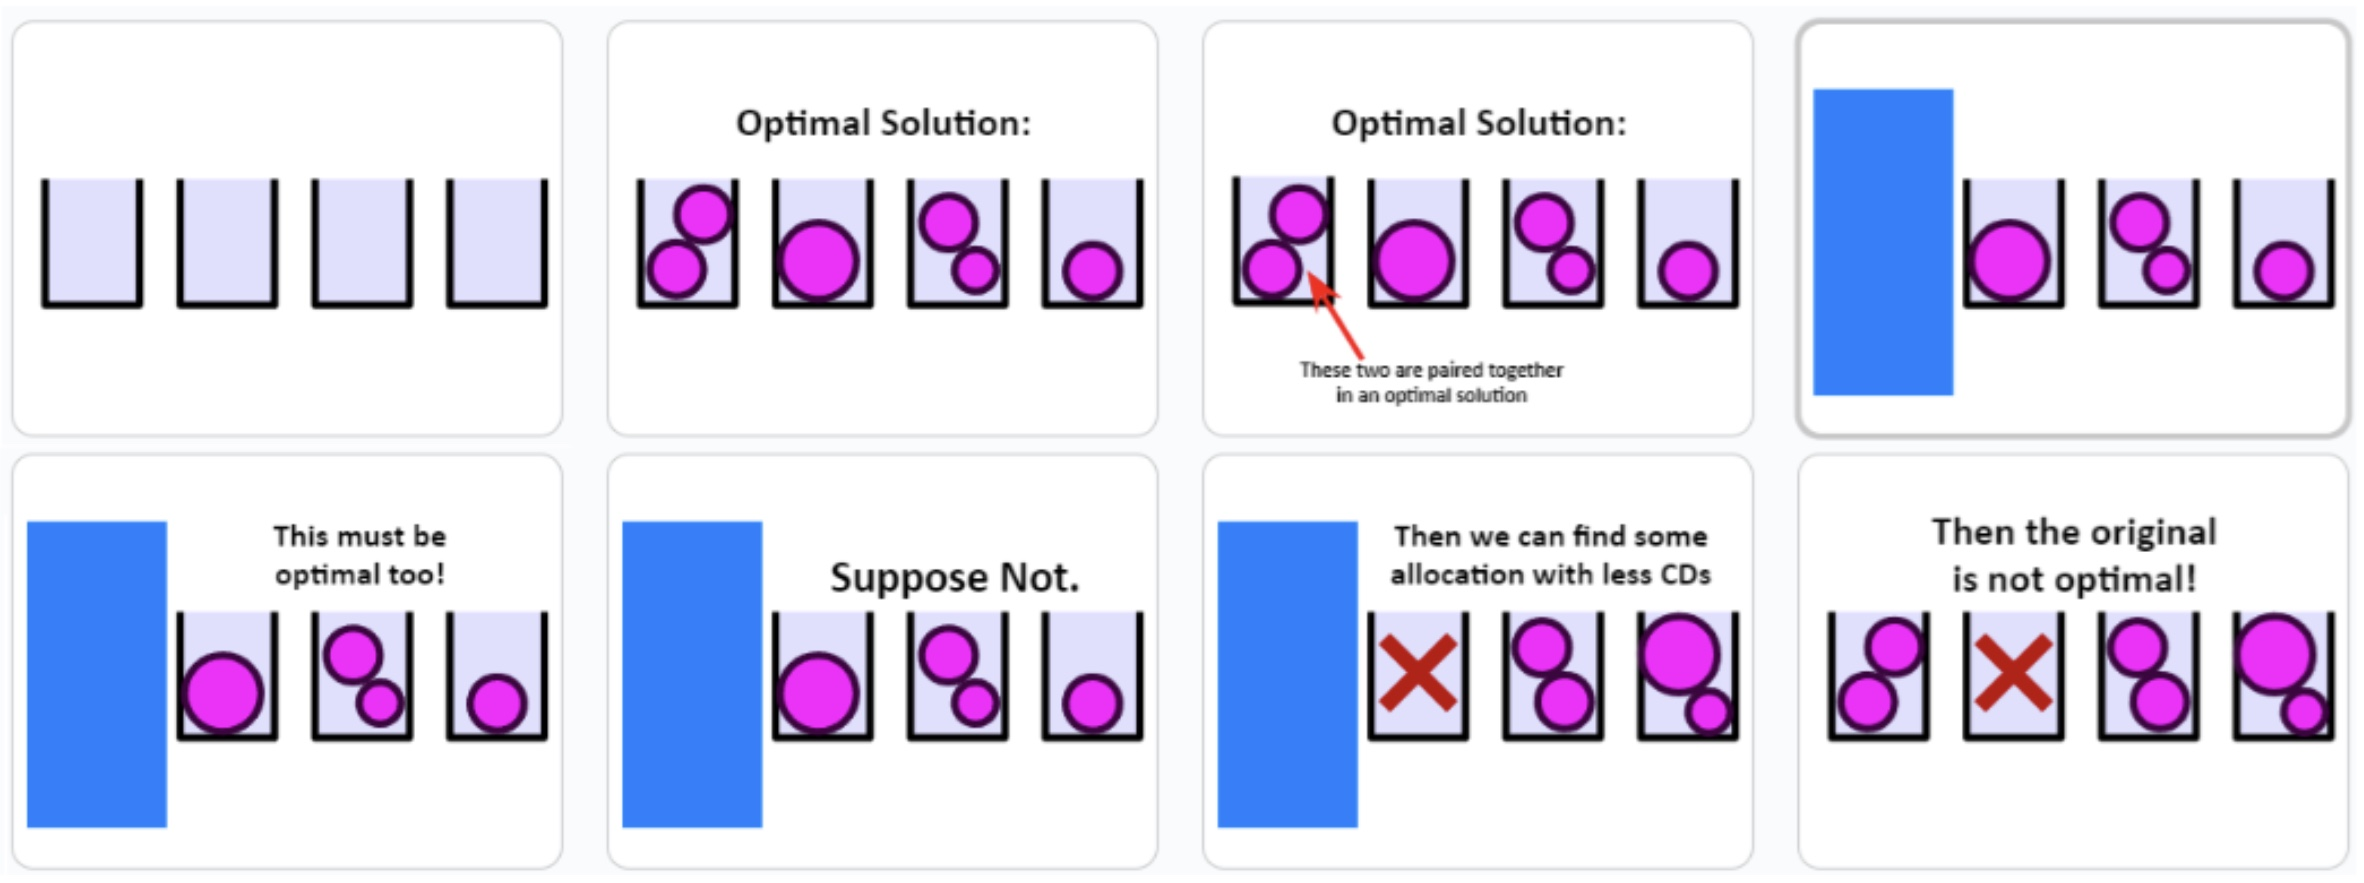
\includegraphics[width=0.6\linewidth]{op.jpeg}
  \caption{Caption.}
\end{figure}


\paragraph{Greedy choice: the smallest file must appear in a pair.}
If the smallest file $f$ is not paired in some optimal solution, choose any pair
$\{a,b\}$ in that solution. Since $f\le a$ and $a+b\le 100$, we also have 
$f+b\le 100$. Swapping $a$ and $f$ preserves feasibility and does not increase
the number of CDs. Hence there exists an optimal solution in which $f$ is in a
pair.
\begin{figure}[h]
  \centering
  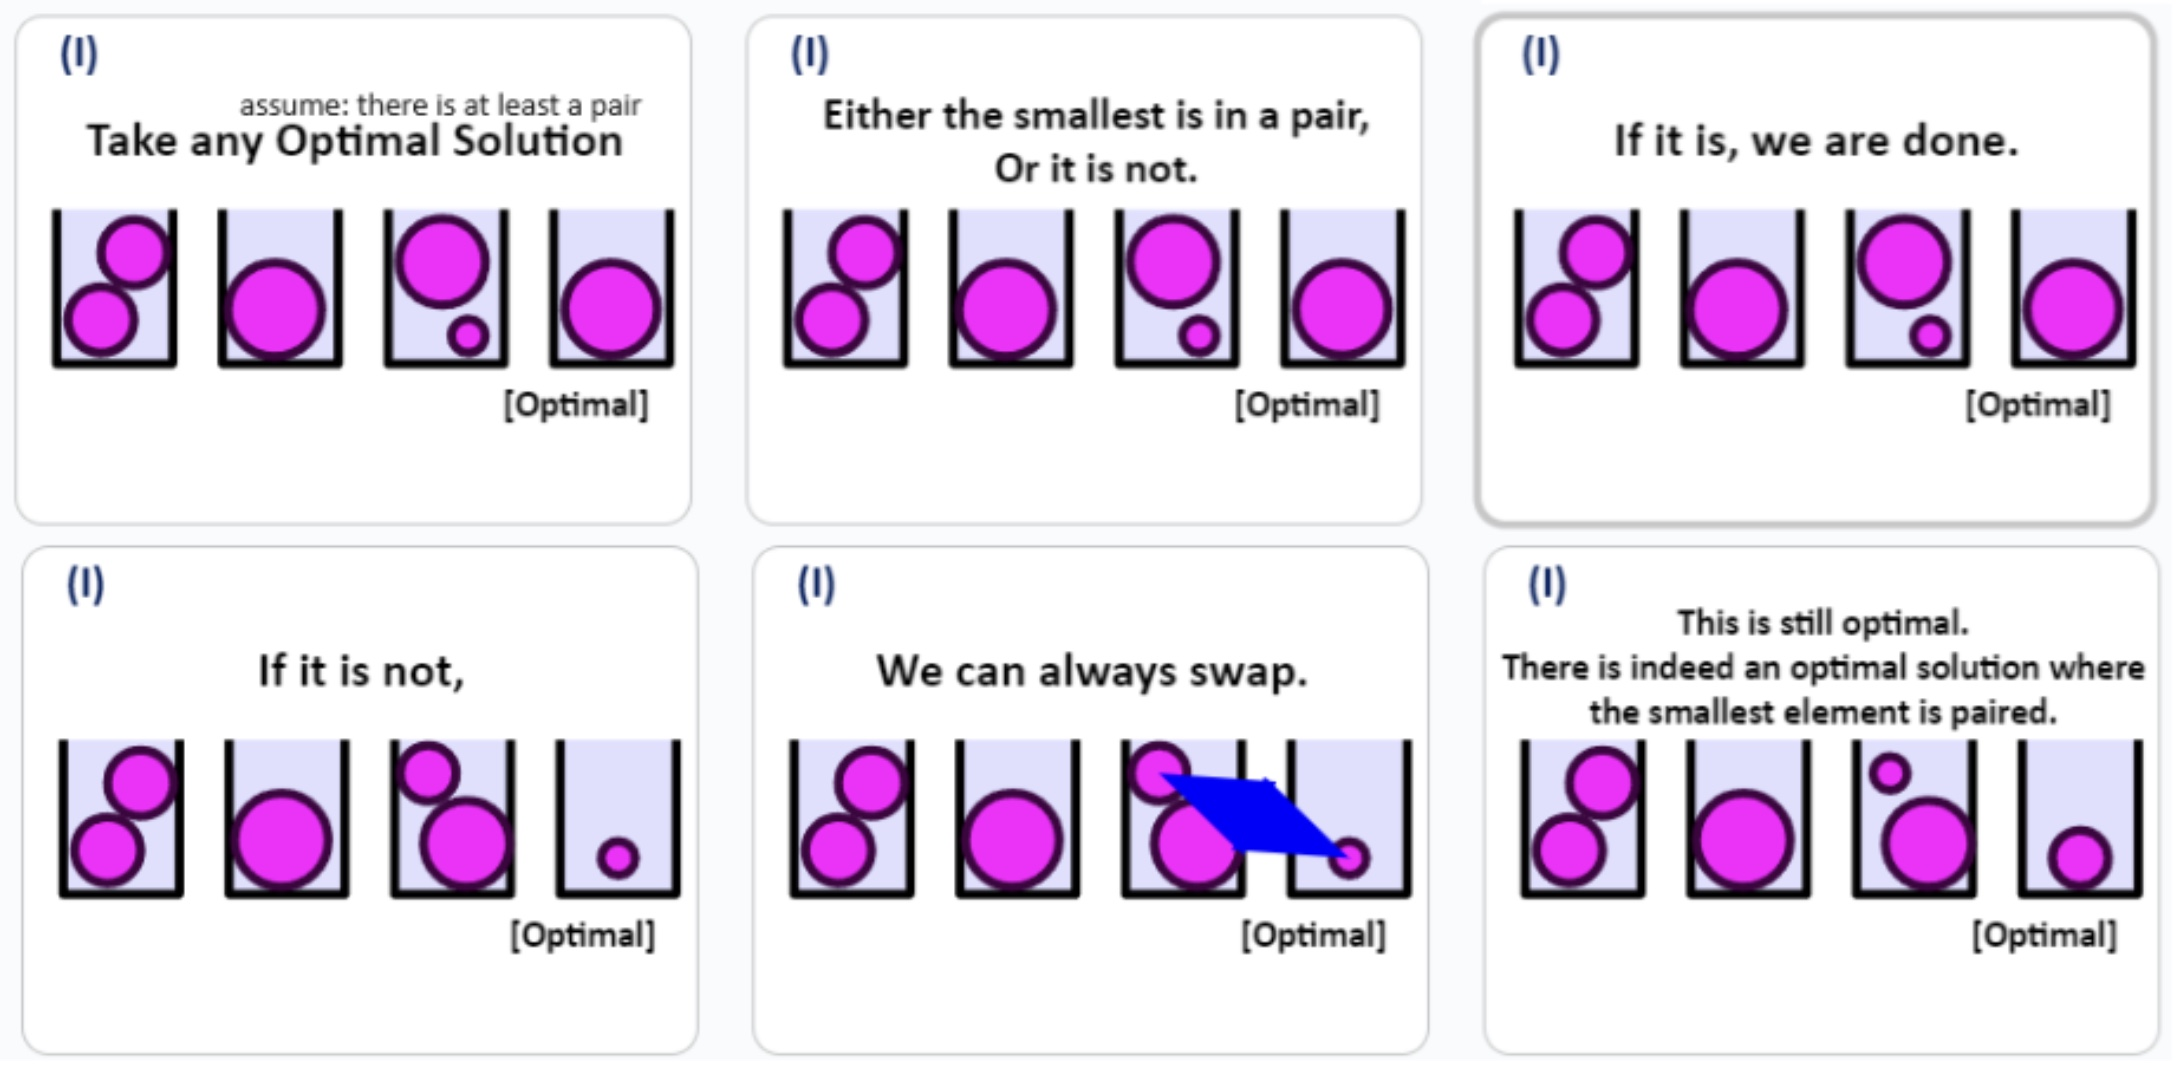
\includegraphics[width=0.6\linewidth]{opss.jpeg}
  \caption{Caption.}
\end{figure}
\paragraph{Greedy choice: pair the smallest file with the largest file that fits.}
Let $f_1$ be the smallest file and let $f_2$ be the largest file such that
$f_1+f_2\le 100$. In any optimal solution where $f_1$ is paired with some other
file $g<f_2$, we may swap $g$ with $f_2$:
\begin{itemize}
    \item if $f_2$ is unpaired, the swap is trivially feasible;
    \item if $f_2$ is paired with another file $h$, then since $f_2>g$, the
          feasibility of $\{g,h\}$ implies $\{f_2,h\}$ also fits.
\end{itemize}
\begin{figure}[h]
  \centering
  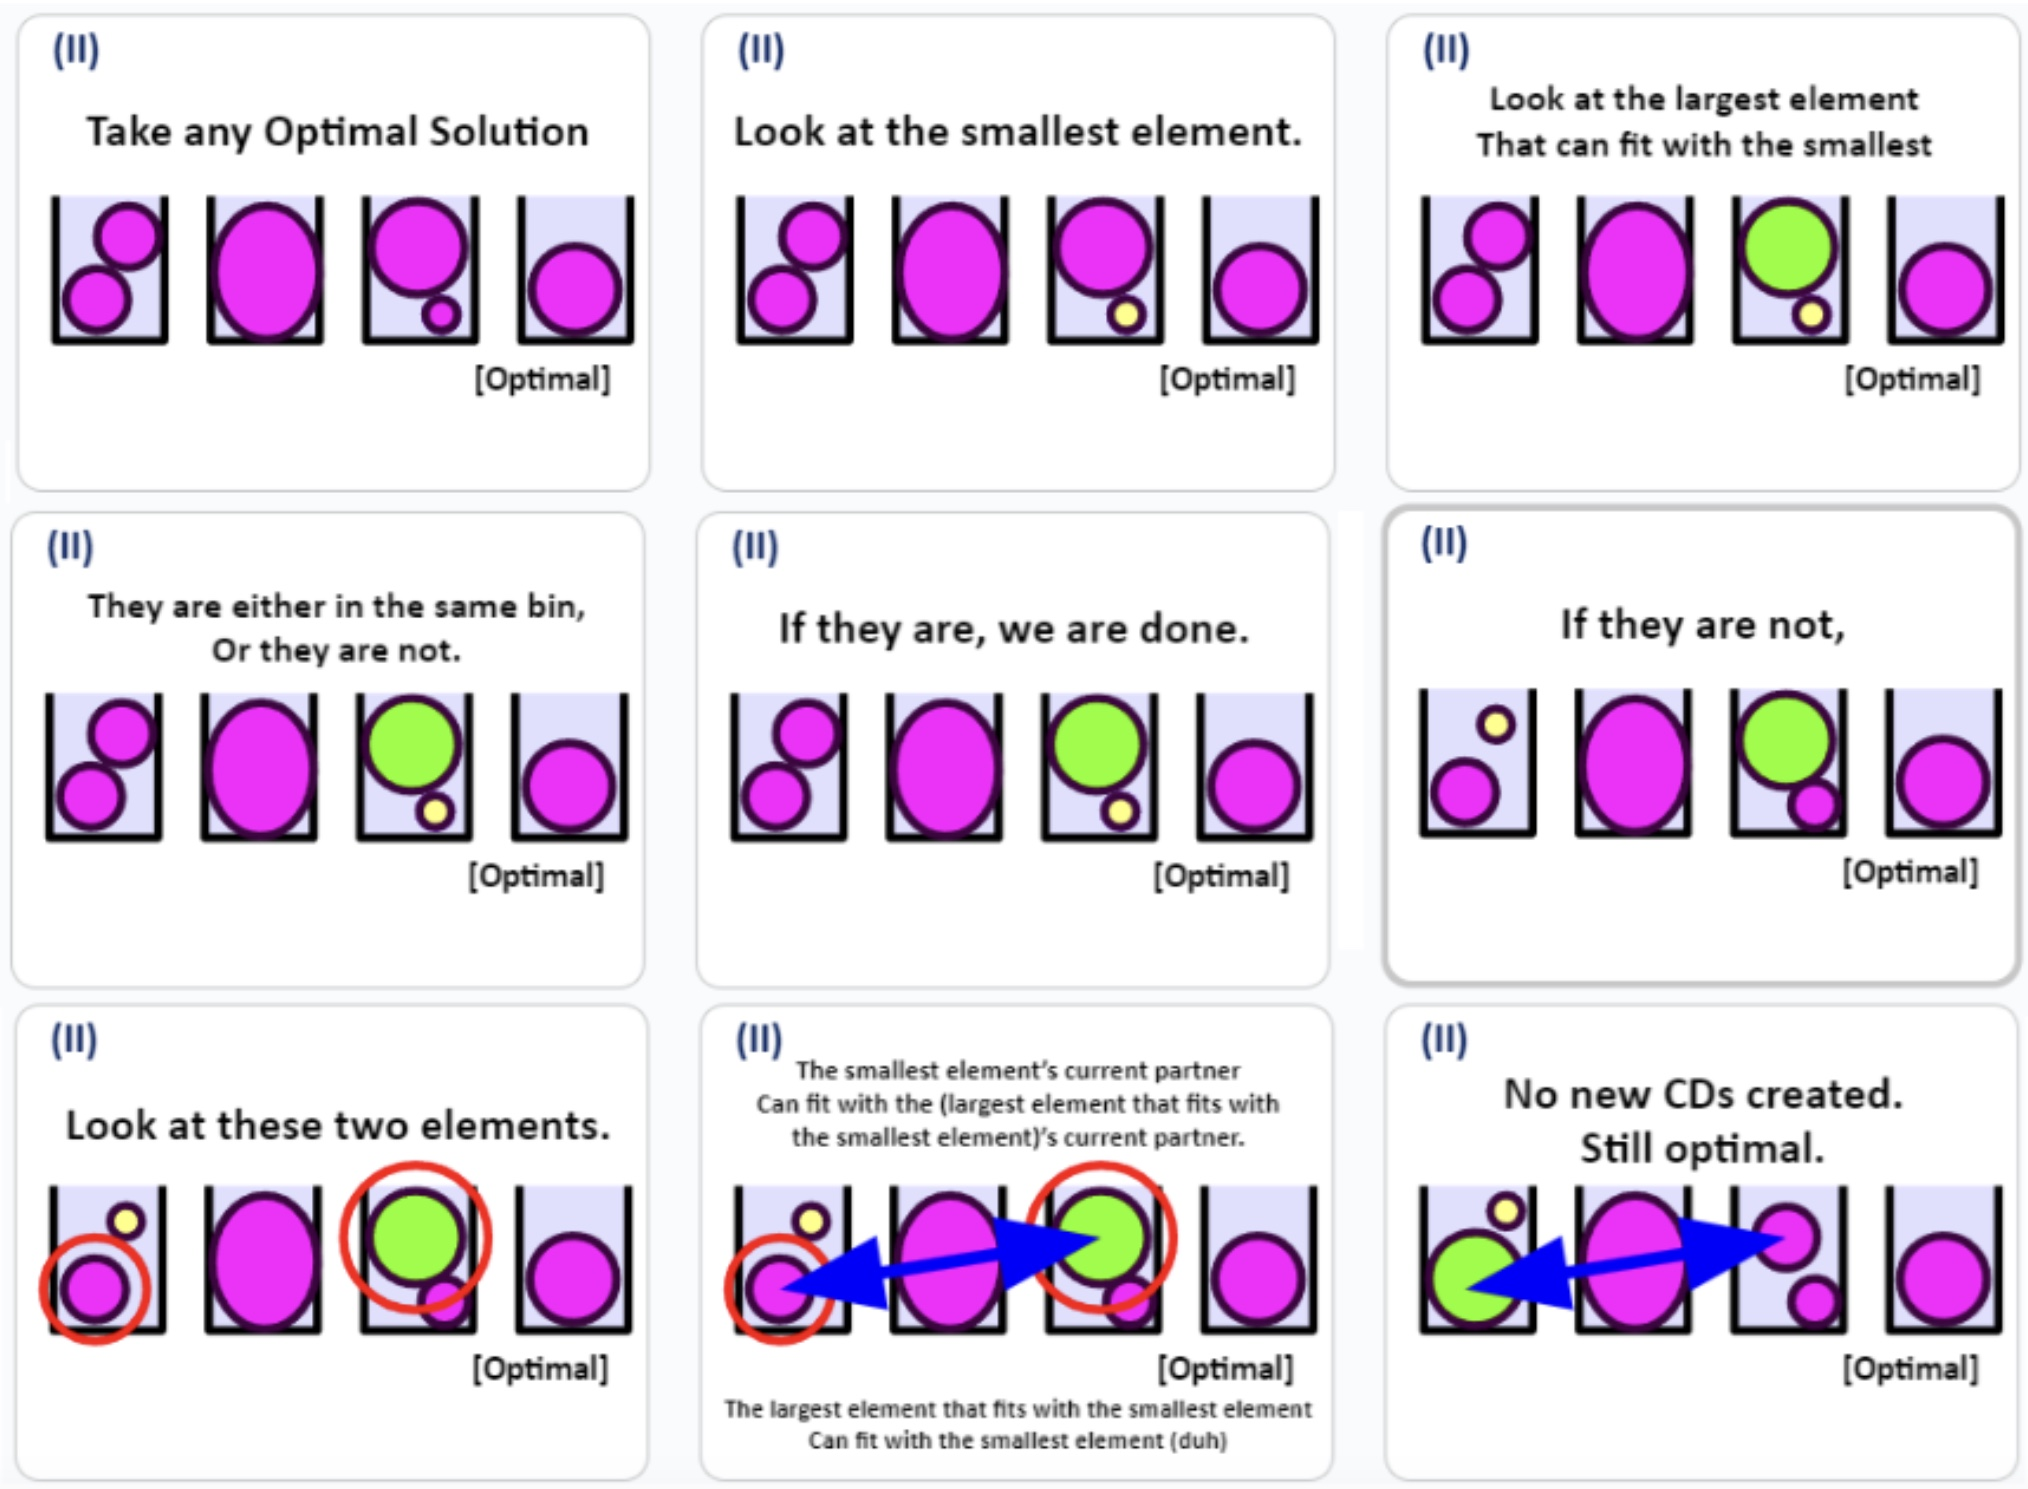
\includegraphics[width=0.6\linewidth]{ops.jpeg}
\end{figure}

Thus an optimal solution exists that contains the greedy pair $\{f_1,f_2\}$.
\newpage
\paragraph{Conclusion.}
Sorting the files and repeatedly pairing the smallest remaining file with the
largest file that fits is a safe greedy choice.  The exchange argument guarantees
that any optimal solution can be transformed into one that makes the greedy
choice.
\subsubsection{Analysis of Statements for the CD Burning Problem}

We are given a set of file sizes 
\(
A = \{a_1, a_2, \dots, a_n\}
\)
sorted so that 
\(
a_1 \ge a_2 \ge \cdots \ge a_n > 0
\),
and a value \(k \ge \lceil |A|/2 \rceil\).
Each CD holds at most two files, and 
\(\mathrm{MinSizeCD}(A,k)\) denotes the minimum CD capacity needed so that \(k\) CDs suffice.

We evaluate the correctness of the following statements:

\begin{enumerate}

\item 
\emph{If \(MinSizeCD(A,k) = a_1\), then \(k = |A|\).}

This is false. Even if the capacity equals the largest file size \(a_1\), 
the remaining files might be small enough to be paired efficiently.
For example, in 
\(A = \{10,1,1,1,1\}\),
capacity \(10\) needs fewer than \(|A|\) CDs.

\item 
\emph{If \(|A|\) is even and \(k = |A|/2\), then \(\mathrm{MinSizeCD}(A,k) = a_1 + a_n\).}

This is false.  
Counterexample:
\(
A = \{5,4,3,1\}
\)
and \(k = 2\).
One might expect capacity \(5+1 = 6\), but the optimal packing is
\((5),(4,3)\), requiring capacity \(7\).  
Thus the stated equality does not hold.

\item 
\emph{If $MinSizeCD(A,k) = a_1 + a_n$, then \(k = |A|/2\).}

Also false.  
Using the same set 
\(A = \{5,4,3,1\}\), 
capacity \(6 = 5+1\) would require \(k = 3\) CDs, not \(2 = |A|/2\).
Hence the implication does not hold.

\item 
\emph{If \(k > |A|/2\), then}
\[
\mathrm{MinSizeCD}(A,k)
= \max\{\,a_1,\ \mathrm{MinSizeCD}(A \setminus \{a_1\},\ k-1)\}.
\]

This statement is true.  
Since \(k > |A|/2\), in any feasible solution at least one CD must contain only one file.  
By a cut-and-paste argument, we can assume without loss of optimality that this single-file CD contains the largest file \(a_1\).  
Thus the optimal capacity is the maximum of \(a_1\) and the optimal capacity for the remaining files with \(k-1\) CDs.

\item 
\end{enumerate}

\noindent
\textbf{Conclusion:} The correct choice is \textbf{(d)}.
\subsection{Maximizing Profit in the Fish Selling Problem}

We are given \(n\) fishes with weights \(w_1, w_2, \ldots, w_n\) and \(m\) fish sellers,
where seller \(j\) is described by a pair \((x_j, p_j)\): he is willing to buy up to
\(x_j\) fishes at price \(p_j\) SGD per kilogram. The goal is to maximize the total
profit from selling (some or all) of the fishes.

\subsubsection*{Optimal Substructure}
Suppose we sell fish \(i\) (weight \(w_i\)) to seller \(j\) who currently has quota
\((x_j, p_j)\). We gain \(w_i p_j\) SGD, fish \(i\) is removed, and the seller state
becomes \((x_j - 1, p_j)\); if \(x_j - 1 = 0\), seller \(j\) is removed.

We claim that the remaining subproblem must be solved optimally. If not, and some
other solution yields higher profit, we could append the sale of fish \(i\) to
seller \(j\), contradicting optimality. Hence the problem has optimal substructure.

\subsubsection*{Greedy Choice and Exchange Argument}
Sort all fishes by non-increasing weight and all sellers by non-increasing price.
Let fish \(i\) be the heaviest available, and seller \(j\) the seller with the
highest price \(p_j\). We claim that there exists an optimal solution in which
fish \(i\) is sold to seller \(j\).

We analyze all possible configurations in an optimal solution:
\begin{enumerate}
    \item If fish \(i\) is already sold to seller \(j\), we are done.
    \item If seller \(j\) buys some fish \(i' \neq i\), and \(i\) is sold to some
          seller \(j'\), then since \(w_{i'} \le w_i\) and \(p_{j'} \le p_j\),
          exchanging assignments of \(i\) and \(i'\) does not decrease profit.
    \item If seller \(j\) buys nothing and fish \(i\) is sold to another seller \(j'\),
          switching fish \(i\) to seller \(j\) increases or preserves profit since
          \(p_{j'} \le p_j\).
    \item If seller \(j\) buys some fish \(i'\) and fish \(i\) is unsold, we can sell
          \(i\) to seller \(j\) instead without losing profit.
    \item The case where seller \(j\) buys nothing and fish \(i\) is unsold is impossible:
          selling fish \(i\) to seller \(j\) increases total profit.
\end{enumerate}
In all cases, there exists an optimal solution selling the heaviest fish to the
highest-paying seller. This establishes the greedy-choice property.

\subsubsection*{Greedy Algorithm}
\begin{enumerate}
    \item Sort fishes by non-increasing weight.
    \item Sort sellers by non-increasing price.
    \item Repeatedly sell the next heaviest fish to the available seller with the
          highest price per kilogram (reduce seller quota by 1; remove seller if
          quota becomes zero).
\end{enumerate}
Because we process each fish once and seller quotas only shrink, the greedy
procedure performs \(O(n)\) assignments.

\subsubsection*{Time Complexity}
Sorting fishes and sellers takes \(O(n \log n + m \log m)\). The greedy matching
step processes at most \(n\) fishes and is \(O(n)\). Hence the full algorithm runs in
\[
O(n \log n + m \log m),
\]
which is polynomial time. Importantly, we never expand seller quotas explicitly
(e.g., repeating a seller \(x_j\) times), which avoids pseudo-polynomial complexity.

\subsubsection*{Conclusion}
The problem admits optimal substructure and a valid greedy-choice property.
Sorting by weight and price and greedily pairing the heaviest fish with the
highest-paying seller yields an optimal solution in polynomial time.

\subsection{Activity Selection Problem}

Each activity $a_i$ occupies an interval $[s_i,f_i)$, and the goal is to select
the maximum number of pairwise compatible activities.

\paragraph{Optimal substructure.}
If an optimal schedule $S$ contains an activity $a_j$, then the activities that
finish before $s_j$ (call this set Before$_j$) and the activities that start
after $f_j$ (call this set After$_j$) must each form an optimal schedule for
their respective subproblems.  Otherwise, replacing either part with a strictly
better solution yields a contradiction of optimality.

\paragraph{Greedy choice: choose the activity that starts last.}
Let $a^*$ be the activity with the latest start time among all activities.  Let
$S$ be an optimal schedule, and let $a$ be the activity in $S$ that starts last
(within $S$).  Since $a^*$ starts no earlier than $a$, replacing $a$ with $a^*$
preserves compatibility with all other activities in $S$.  This exchange
preserves the size of the schedule, so the modified schedule remains optimal.
Therefore every optimal solution can be made to include $a^*$.

\paragraph{Conclusion.}
Processing activities in decreasing order of start times and greedily selecting
each compatible activity is a safe greedy strategy.  The exchange argument shows
that the latest-starting activity is always part of some optimal solution.
\subsection{Dominating Set Variant of the Activity Selection Problem}

We are given \(A = \{a_1, a_2, \ldots, a_n\}\), where activity
\(a_i = [s_i, f_i)\) with \(s_i < f_i\).
Two activities overlap if their time intervals intersect. 
A subset \(D \subseteq A\) is \emph{dominating} if for every activity
\(a_i \in A \setminus D\), there exists \(a_j \in D\) such that 
\(a_i\) and \(a_j\) overlap.
Our goal is to compute a smallest dominating subset.

\subsubsection*{Incorrect Greedy Algorithm}
A natural attempt is to repeatedly pick an activity that covers (overlaps)
the largest number of uncovered activities:
\begin{enumerate}
    \item \(D \leftarrow \emptyset\); \(B \leftarrow A\).
    \item While \(B \neq \emptyset\):
    \begin{enumerate}
        \item Select \(a \in A \setminus D\) maximizing the number of activities
              in \(B\) that overlap with \(a\).
        \item Add \(a\) to \(D\).
        \item Remove from \(B\) all activities that overlap with \(a\).
    \end{enumerate}
    \item Return \(D\).
\end{enumerate}

This algorithm is \emph{incorrect}.  
A counterexample is:
\[
A = \{[1,2), [1,3), [2,3), [2,4), [3,4), [3,5), [4,5)\}.
\]
An optimal dominating set is
\[
D^* = \{[1,3), [3,5)\}.
\]
However, the greedy algorithm first selects \([2,4)\) (it overlaps the most
intervals) and is then forced to take two additional intervals, producing
a strictly larger dominating set.

Common mistakes include:
(i) choosing from \(A \setminus D\) rather than from \(B\),
(ii) maximizing instead of minimizing,
(iii) treating lengths instead of number of activities,
(iv) attempting a proof without a counterexample.

\subsubsection*{Correct Polynomial-Time Greedy Algorithm}
We modify the greedy choice as follows:
\begin{enumerate}
    \item Select \(a_i = [s_i, f_i) \in B\) with the \emph{minimum} finish time.
    \item Let \(S\) be all activities in \(A \setminus D\) that overlap with \(a_i\).
    \item From \(S\), select \(a_j = [s_j, f_j)\) with the \emph{maximum} finish time.
    \item Add \(a_j\) to \(D\), remove all activities in \(B\) overlapping with \(a_j\).
\end{enumerate}

This greedy rule is correct:  
in any optimal dominating set, some activity in \(S\) must be chosen,
otherwise \(a_i\) would be undominated. If the optimal solution chooses
\(a_k \in S\), then replacing \(a_k\) by \(a_j\) (the one with maximum
finish time) still dominates all activities that \(a_k\) dominated.
If an activity overlapped with \(a_k\) but not with \(a_j\), then:
\begin{itemize}
    \item either it finishes before \(s_j\), contradicting the fact that
          \(f_i\) was the minimum finish time, or
    \item it starts after \(f_j \ge f_k\), meaning it does not overlap
          with \(a_k\) either.
\end{itemize}
Hence \(a_j\) is always safe to choose.

A simpler interpretation:
\begin{itemize}
    \item Pick the earliest-finishing uncovered interval \(x\).
    \item Among all activities that overlap \(x\), pick one that finishes as \emph{late} as possible.
\end{itemize}

Equivalent variations include:
(i) replacing ``finishes first'' with ``starts first'',
(ii) replacing ``maximum finish time'' with ``maximum number of uncovered overlaps''.
However, both modifications cannot be done simultaneously.

\subsubsection*{Notes and Common Pitfalls}
\begin{itemize}
    \item Minimum dominating set is \emph{not} maximum independent set.
    \item Tie-breaking rules alone cannot fix the incorrect greedy strategy.
    \item Selecting the longest interval or earliest/last start/finish time alone is incorrect.
    \item The algorithm runs in polynomial time: sorting plus linear scanning.
\end{itemize}



\newpage
\section{Amortization Analysis}
\subsection{Aggregate method}
\subsection{Accounting method}
Charge the $i_{th}$ operation a fictitious amortized cost $c(i)$, assuming 1 cost is paid for 1 unit of work. This fee is consumed to perform
the operation and any amount that is not immediately consumed goes into a bank to be used by subsequent potentially costly operations. Invariant: the bank
balance can never go negative.
\[\forall n, \sum_{i=1}^{n} t(i) \leq \sum_{i=1}^{n} c(i)\]
This ensure the total amortized cost provides an upper bound on the total true cost.
\subsubsection*{Example: \texttt{INSERT} in dynamic table}
Still we use double upon full. Instead of a cost of 1 for 1 insertion operation, we impose a fictitious cost of 3. We need to prove that 
\begin{align*}
  &\forall n\in \mathbb{N}, \sum_{i=1}^{n} t(i) \leq \sum_{i=1}^{n} c(i)\\
  &\forall n \in \mathbb{N}, n + \sum_{i=1}^{\lfloor \log_2(n)\rfloor} 2^i \leq \sum_{i=1}^{n} 3  
\end{align*}
\begin{proof}
LHS = $n + (2^{\lfloor \log_2(n)\rfloor + 1} - 2)$, $2^{\lfloor \log_2(n)\rfloor + 1} \leq 2n$, LHS $< 3n$ = RHS
\end{proof}
\subsection{Potential method}
Let $\phi(i)$ be the potential at the end of $i^{th}$ operation, if we maintain invariants
\begin{align*}
  \phi(0) &= 0\\
  \phi(i) &\geq 0, \forall i
\end{align*}
The amortized cost of the $i_{th}$ operation is defined as the actual cost plush the potential 
difference $\Delta \phi(i) = \phi(i) - \phi(i-1)$. \\
The amortized cost of $n$ operation:
\begin{align*}
  \sum_{i} c_{amortized} &= \sum_{i} (t(i) + \phi(i) - \phi(i-1))\\
  &= \sum_{i} t(i) + (\phi(n) - \phi(0))\\
  &= \sum_{i} + \phi(n) 
\end{align*}
\[\sum_{i} c_{amortized} \in O(g(n)) \implies \sum_{i} t(i) \in O(g(n))\]
\subsubsection*{Example: \texttt{Pop()} in dynamic table: half upon resizing} 
Let $\phi(i) = 2(m_i - n_i)$ where $m_i$ is the table size when carrying out the $i^{th}$ operation, and $n_i$ is the number of element in the table. 
\begin{enumerate}
  \item Not resizing:
  \begin{itemize}
    \item Operation cost $c(i) = 1$
    \item $\phi(i) = 2(m - n), \phi(i - 1) = 2(m - (n - 1))$
    \item $\Delta\phi(i) = 2$
  \end{itemize}
  \item Shrinking:
  \begin{itemize}
    \item Operation cost $c(i) = 1 + \frac{m}{2}$
    \item $\phi(i) = 2(m - n), \phi(i - 1) = 2(\frac{m}{2} - (n-1))$
    \item $\Delta \phi(i) = m $
  \end{itemize}
\end{enumerate}
\subsection{Amortized Analysis: Choosing Accounting and Potential Functions}

This subsection summarizes the main conceptual ideas behind amortized analysis
from Tutorial~08.  The focus is on \emph{why} we pick certain amortized charges
(accounting method) or certain potential functions (potential method), and how
these choices guarantee amortized $O(1)$ or $O(n)$ bounds for sequences of
operations.

\subsubsection*{1. Amortized Analysis: Key Idea}
Amortized analysis studies the total cost of a \emph{sequence} of operations.
Even if individual operations may be expensive, we show that:
\[
\frac{\text{Total true cost}}{\text{Total number of operations}}
\]
is small in the worst case.  
Unlike expected-time analysis, no probability is involved: the guarantee is
worst-case per operation over any sequence.

The tutorial emphasizes two methods:
\begin{itemize}
    \item \textbf{Accounting method}: assign a “fictional’’ charge $C(i)$ to
          operation $i$, possibly larger than its true cost $T(i)$.
    \item \textbf{Potential method}: define a potential $\phi$ that measures
          “stored work’’ and use
          \[
          C(i) = T(i) + (\phi(i) - \phi(i-1)).
          \]
\end{itemize}
Both methods ensure the bank balance / potential never goes negative.

\subsubsection*{2. Choosing Accounting Charges}
From the tutorial examples, the pattern is:

\paragraph{(a) Dynamic Table Insertion (doubling).}
We charge \$3 for each insertion:
\[
\text{True cost}=1 \text{ (normal insert)} \quad\text{or}\quad T=\Theta(n)
\text{ (when doubling)}.
\]
The choice “\$3’’ follows the rule:
\[
\textbf{Charge normal operations slightly more, so the saved credits pay for rare expensive ones.}
\]
Because each element moved during a future doubling was once inserted, assigning
an extra \$2 on every insertion exactly accumulates enough credit to pay for all
future copies.  
This makes the amortized cost $O(1)$.

\paragraph{(b) Queue with ENQUEUE/DEQUEUE/DELETE/ADD.}
Each element that enters the queue is charged \$2:
\[
\$1 \text{ to enqueue it} \quad+\quad \$1 \text{ saved for future removal}.
\]
Thus:
\[
\text{ENQUEUE}(x): \$2,\quad \text{DEQUEUE}():\$0,\quad \text{DELETE}(k):\$0,\quad
\text{ADD}(A): 2|A|.
\]
The bank invariant is:  
\emph{every element present in the queue holds exactly \$1 for its eventual
deletion}.  
This ensures DEQUEUE and DELETE are free in the amortized sense.

\subsubsection*{3. Choosing Potential Functions}
The potential method requires a $\phi$ such that:
\[
\phi(0)=0,\qquad \phi(i)\ge 0 \quad \forall i.
\]
The tutorial provides two guiding heuristics:

\paragraph{Heuristic 1: The potential should decrease sharply during expensive operations.}
This makes the amortized cost
\[
C(i)=T(i)+(\phi(i)-\phi(i-1))
\]
small even when $T(i)$ is large.

\paragraph{(a) Queue with ENQUEUE/DEQUEUE/DELETE/ADD.}
A natural potential is:
\[
\phi(i) = \text{current queue size}.
\]
The reasoning:
\begin{itemize}
    \item expensive operations (DELETE, DEQUEUE) shrink the queue,
          so $\phi$ decreases sharply, offsetting the true cost;
    \item cheap operations (ENQUEUE) increase $\phi$ in a controlled way.
\end{itemize}
This yields amortized costs:
\[
\begin{array}{c|c|c|c}
\text{Operation} & T(i) & \phi(i)-\phi(i-1) & C(i) \\
\hline
\text{ENQUEUE} & 1 & +1 & 2 \\
\text{DEQUEUE} & 1 & -1 & 0 \\
\text{DELETE}(k) & k & -k & 0 \\
\text{ADD}(A) & |A| & +|A| & 2|A| \\
\end{array}
\]

\paragraph{(b) Dynamic Table with POP() only (halving).}
The subtle choice:
\[
\phi(i) = \text{number of empty cells } = \text{size}(T) - n.
\]
Why this works:
\begin{itemize}
    \item Before halving, the table has many empty cells, so $\phi$ is large.
    \item After halving, $\phi$ \emph{drops dramatically}, offsetting the heavy
          cost of copying.
    \item When POP does not trigger halving, $\phi$ increases slightly.
\end{itemize}

The amortized analysis table:
\[
\begin{array}{c|c|c|c}
\text{Operation} & T(i) & \phi(i)-\phi(i-1) & C(i) \\
\hline
\text{Normal POP} & 1 & +1 & 2 \\
\text{POP that halves} & n+1 & -(n-1) & 2 \\
\end{array}
\]
Hence amortized $O(1)$.

\subsubsection*{4. Key Takeaways for Designing Amortized Proofs}

\begin{itemize}
    \item \textbf{Find the invariant:}  
          Which quantity is preserved or slowly built up?  
          (e.g., each inserted element stores enough money for its own copying or deletion.)

    \item \textbf{Account or store potential on the cheap, spend on the expensive:}  
          The expensive operations should cause a large decrease in stored credit/potential.

    \item \textbf{Potential often matches “unused capacity’’ or “queue length’’:}  
          For dynamic tables: unused slots.  
          For queues: number of elements.  
          For stacks/monotonic structures: stack height.

    \item \textbf{Amortization is about sequences, not single operations:}  
          Even if one step is $\Theta(n)$, the average stays $O(1)$.
\end{itemize}

\paragraph{Summary.}
The central goal in both accounting and potential methods is to choose an
amortized cost or potential that tracks a “stored resource’’ which accumulates
during cheap operations and is spent during expensive ones.  
This ensures the total amortized cost upper-bounds the total true cost for any
operation sequence.

\subsection{Amortized Analysis of Dynamic Hash Tables with Rehashing}

We maintain a hash table of size \(M\) with \(N\) stored keys, using Separate
Chaining. The load factor is
\[
\alpha = \frac{N}{M},
\]
which determines the expected chain length. To keep \(\alpha\) bounded by a
constant, we apply the following resizing rules:
\begin{itemize}
    \item \textbf{Doubling}: If an insertion causes \(\alpha > 2\), we double
          the table size from \(M\) to \(2M\) and rehash all \(N\) keys.
    \item \textbf{Halving}: If a deletion causes \(\alpha < \tfrac12\), we halve
          the table size from \(M\) to \(M/2\) and rehash all \(N\) keys.
\end{itemize}
Each rehash takes \(\Theta(N)\) time. We assume (as permitted) that every
individual insertion or deletion takes at most \(\alpha + 1 = O(1)\) time when
no rehash occurs. The goal is to prove that \textbf{amortized} cost of both
insertion and deletion remains \(O(1)\).

\subsubsection*{Potential Function}
Define the potential function:
\[
\phi = 2|N - M| + 2.
\]
This potential reflects how far the table size \(M\) deviates from the number
of keys \(N\).

\subsubsection*{No-Rehash Case}
If no resizing occurs, \(M\) stays the same and \(N\) changes by exactly \(1\).
Hence
\[
\Delta \phi \le 2.
\]
The amortized cost is
\[
\text{amortized} = \text{actual} + \Delta \phi \le 1 + 2 = 3,
\]
a constant.

\subsubsection*{Doubling Rehash}
A doubling rehash occurs when an insertion causes \(\alpha > 2\), meaning
\(M = N/2\) just before the rehash. After rehashing, the table size becomes
\(M' = N\), and the insertion increases \(N\) to \(N+1\).

Before rehash:
\[
\phi(i-1) = 2|N - N/2| + 2 = 2 \cdot \tfrac{N}{2} + 2 = N + 2.
\]
After rehash:
\[
\phi(i) = 2|(N+1) - (N+1)| + 2 = 2.
\]
Thus:
\[
\Delta \phi = 2 - (N + 2) = -N.
\]
Actual cost of rehashing all \(N\) items plus the insertion is \(N + 1\).
So amortized cost:
\[
(N+1) + (-N) = 1.
\]
This is bounded by a constant (in the official solution they simplify it to \(3\)).

\subsubsection*{Halving Rehash}
A halving rehash occurs when a deletion causes \(\alpha < \tfrac12\), meaning
\(M = 2N\) before deletion. After the deletion we have \(N' = N-1\) and the
table size becomes \(M' = N-1\).

Before rehash:
\[
\phi(i-1) = 2|N - 2N| + 2 = 2N + 2.
\]
After rehash:
\[
\phi(i) = 2|(N-1)-(N-1)| + 2 = 2.
\]
Thus:
\[
\Delta \phi = 2 - (2N + 2) = -2N.
\]
The actual cost of rehashing \(N-1\) keys plus the deletion is \(N\), so
amortized cost:
\[
N + (-2N) = -N,
\]
which is again \(O(1)\); following the instructor’s simplified bound, this is
treated as at most \(3\).\\
The amortized analysis table:
\[
\begin{array}{c|c|c|c}
\text{Operation} & T(i) & \phi(i)-\phi(i-1) & C(i) = T(i)+\Delta\phi \\
\hline
\text{Insert/Delete (no rehash)} & 1     & \le 2     & \le 3 \\
\text{Insert causing doubling}   & N+1   & 2 - N     & 3    \\
\text{Delete causing halving}    & N+1   & 2 - N     & 3    \\
\end{array}
\]
Hence each operation has amortized cost $O(1)$.

\subsubsection*{Conclusion}
In every case---ordinary insertion/deletion, doubling, or halving---the
amortized cost is at most a constant. Therefore:
\[
\boxed{\text{Amortized cost of insertion and deletion is } O(1).}
\]
This holds even though resizing (rehashing all keys) is an expensive
\(\Theta(N)\)-time operation.
\subsection{Amortized Analysis of Data Structures via the Potential Method}

\subsubsection*{Potential Method: Reminder}
Let $D_i$ be the data structure state after the $i$-th operation, with real cost $c_i$.
A \emph{potential function} is a mapping
\[
  \Phi : \{ \text{states} \} \to \mathbb{R}_{\ge 0}
\]
such that $\Phi(D_0) = 0$ and $\Phi(D_i) \ge 0$ for all $i$.
The \emph{amortized cost} of operation $i$ is defined as
\[
  \hat c_i \;=\; c_i + \Phi(D_i) - \Phi(D_{i-1}).
\]
Summing over $i=1,\dots, m$ gives
\[
  \sum_{i=1}^m \hat c_i
  \;=\; \sum_{i=1}^m c_i \;+\; \Phi(D_m) - \Phi(D_0)
  \;\ge\; \sum_{i=1}^m c_i,
\]
so the total amortized cost provides an upper bound on the total real cost.

\subsubsection{Self-Adjusting Binary Search Tree (Splay Tree)}

\paragraph{Model.}
We consider a \emph{splay tree}, a self-adjusting binary search tree that performs
a \emph{splay} (a sequence of rotations) after each access.
We analyze operations \textsc{Search}, \textsc{Insert}, and \textsc{Delete}
in terms of amortized time.

Plain (unbalanced) BSTs have no non-trivial worst-case or amortized guarantees
for arbitrary sequences of operations, so we explicitly assume the splay tree variant.

\paragraph{Size and Rank.}
For each node $x$, let $s(x)$ be the size (number of nodes) in the subtree rooted at $x$.
Define the rank of $x$ as
\[
  r(x) \;=\; \log s(x),
\]
and let the potential of a tree $T$ be
\[
  \Phi(T) \;=\; \sum_{x \in T} r(x)
             \;=\; \sum_{x \in T} \log s(x).
\]
Clearly $\Phi(T) \ge 0$ and $\Phi(\emptyset) = 0$.

\paragraph{Single Splay Step.}
A splay consists of a sequence of rotations, each of which is a \emph{zig}, \emph{zig-zig}, or \emph{zig-zag} step.
The real cost of each step is $O(1)$ (constant-time pointer updates).

One proves the \emph{Access Lemma}: splaying node $x$ to the root has amortized cost
\[
  O\bigl( 1 + r(T) - r(x) \bigr)
  \;=\; O\bigl( 1 + \log n - \log s(x) \bigr),
\]
where $n = |T|$ and $r(T)$ is the rank of the root.
The proof is a case-by-case analysis over zig, zig-zig, and zig-zag:
in each case we bound
\[
  \hat c_{\text{step}}
  \;=\; c_{\text{step}} + \Phi(\text{after}) - \Phi(\text{before})
\]
using the ranks of the nodes involved and the fact that logarithms smooth out subtree size changes.
The total potential increase over all steps in a splay is then telescoped and bounded.

\paragraph{Amortized Cost of Operations.}
\begin{itemize}
  \item \textsc{Search}$(x)$: perform standard BST search, then splay $x$ (or the last accessed node) to the root.  
  Amortized cost: $O(\log n)$ by the Access Lemma.

  \item \textsc{Insert}$(x)$: insert $x$ as in a standard BST (cost $O(\text{depth}(x))$),
  then splay $x$ to the root.
  The splay dominates the cost, so amortized cost: $O(\log n)$.

  \item \textsc{Delete}$(x)$: splay $x$ to the root, delete it, and re-join the two subtrees
  (e.g.\ splay the maximum of the left subtree to the root and attach the right subtree).
  Each splay is $O(\log n)$ amortized, so overall amortized cost is $O(\log n)$.
\end{itemize}

Thus, under this potential function, all basic operations on a splay tree have amortized time $O(\log n)$.

\subsubsection{Binary Heap Priority Queue}

\paragraph{Model.}
Consider a binary heap implementing a priority queue with operations:
\textsc{Insert}, \textsc{Extract-Min}, and \textsc{Decrease-Key}.
We store $n$ elements in an array-based heap.

\paragraph{Trivial Potential.}
Since each operation is already $O(\log n)$ in the worst case, one can use a very simple potential,
e.g.\ $\Phi(H) = 0$ for all states $H$, or more critically
\[
  \Phi(H) = c \cdot n
\]
for some constant $c > 0$.
This potential does \emph{not} change asymptotic bounds, but lets us formally express amortized costs.

\paragraph{Amortized Costs.}
\begin{itemize}
  \item \textsc{Insert}: place the new element at the end of the array and \emph{bubble up} along at most $\lfloor \log n \rfloor$ levels.  
  Real cost $c_i = O(\log n)$; potential change $\Phi(H_i)-\Phi(H_{i-1}) = O(1)$
  (only $n$ changes by $1$).  
  Therefore $\hat c_i = O(\log n)$.

  \item \textsc{Extract-Min}: swap the root with the last element, remove the last element,
  then \emph{bubble down} along at most $\lfloor \log n \rfloor$ levels.  
  Again $c_i = O(\log n)$ and $|\Phi(H_i)-\Phi(H_{i-1})|=O(1)$, so $\hat c_i = O(\log n)$.

  \item \textsc{Decrease-Key}: bubble up similarly to \textsc{Insert}, touching at most
  $O(\log n)$ nodes.  
  Same reasoning yields $\hat c_i = O(\log n)$.
\end{itemize}

Here the potential method is mostly a formal confirmation that nothing pathological happens
over a long sequence of heap operations; the amortized bounds match the worst-case bounds.

\subsubsection{Fibonacci Heap}

\paragraph{Model.}
A Fibonacci heap is a priority queue supporting:
\begin{itemize}
  \item \textsc{Insert},
  \item \textsc{Find-Min},
  \item \textsc{Union} (meld two heaps),
  \item \textsc{Extract-Min},
  \item \textsc{Decrease-Key},
  \item \textsc{Delete}.
\end{itemize}
It maintains a collection of heap-ordered trees in a root list,
and uses \emph{lazy} consolidation plus \emph{cascading cuts}.

Let:
\begin{itemize}
  \item $t(H)$ = \# of trees in the root list of heap $H$,
  \item $m(H)$ = \# of \emph{marked} nodes (nodes that have lost a child since they became a child themselves).
\end{itemize}

\paragraph{Potential Function.}
Define
\[
  \Phi(H) = t(H) + 2 m(H).
\]
This is always non-negative; a newly created empty heap has $\Phi = 0$.

\paragraph{Operation Analyses.}

\textbf{Insert$(x)$}.  
We create a singleton tree containing $x$ and add it to the root list.

\begin{itemize}
  \item Real cost $c_i = O(1)$.
  \item $t(H)$ increases by $1$, $m(H)$ unchanged, so $\Phi(H_i)-\Phi(H_{i-1}) = 1$.
  \item Amortized cost:
    \[
      \hat c_i = c_i + \Delta \Phi = O(1) + 1 = O(1).
    \]
\end{itemize}

\textbf{Find-Min}.  
We maintain a pointer to the minimum root in the root list.

\begin{itemize}
  \item Real cost $c_i = O(1)$.
  \item No structural change, so $\Delta \Phi = 0$.
  \item Amortized cost: $\hat c_i = O(1)$.
\end{itemize}

\textbf{Union$(H_1,H_2)$}.  
We concatenate the two root lists and update the min pointer.

\begin{itemize}
  \item Real cost $c_i = O(1)$ (pointer manipulation).
  \item $t(H)$ becomes $t(H_1)+t(H_2)$ and $m$ is unchanged; this is essentially additive and does not increase asymptotics.
  \item Amortized cost: $\hat c_i = O(1)$.
\end{itemize}

\textbf{Extract-Min}.  
Let $z$ be the current minimum root.
We:
\begin{enumerate}
  \item Remove $z$ from the root list.
  \item Add all children of $z$ to the root list (unmarking them).
  \item \emph{Consolidate}: repeatedly link roots of the same degree,
        making the larger-key root a child of the smaller-key root.
\end{enumerate}

The expensive part is consolidation. Let $D(n)$ be the maximum degree of any node in a heap of size $n$ (it can be shown that $D(n)=O(\log n)$).

\begin{itemize}
  \item The real cost $c_i$ is $O(D(n) + t(H))$, which is $O(\log n + t(H))$.
  \item Potential change:
    \begin{itemize}
      \item Removing $z$ decreases $t(H)$ by $1$.
      \item Adding its children to the root list increases $t(H)$ by $\deg(z)$
            and sets their marks to $0$ (reducing $m(H)$ if they were marked).
      \item Each root-link during consolidation decreases $t(H)$ by $1$
            and may change marks only by a constant.
    \end{itemize}
    Overall, one can show
    \[
      \Delta \Phi \;=\; \Phi(H_i) - \Phi(H_{i-1}) \;\le\; O(\log n) - \Omega(t_{\text{before}}),
    \]
    so a large amount of structural work (many root links) is paid for by a
    corresponding decrease in potential.
  \item Combining these bounds yields an amortized cost $\hat c_i = O(\log n)$.
\end{itemize}

\textbf{Decrease-Key$(x,\Delta)$}.  
We decrease the key of node $x$ by $\Delta>0$.
If the heap order is violated (i.e.\ $x$ becomes smaller than its parent),
we \emph{cut} $x$ from its parent and add $x$ to the root list.
If the parent was already marked, we repeat this upwards (cascading cuts);
otherwise, we mark the parent.

Let $k$ be the number of nodes cut (including $x$).

\begin{itemize}
  \item Real cost $c_i = O(k)$ (each cut and mark/unmark is $O(1)$).
  \item Potential change:
    \begin{itemize}
      \item Each cut adds one tree ($t(H)$ increases by 1),
            but \emph{unmarks} the cut node (decreasing $m(H)$ by 1).
      \item Marking the parent increases $m(H)$ by 1.
    \end{itemize}
    One can check that each cut reduces $m(H)$ or keeps it bounded,
    and the potential change over $k$ cuts is at most $O(1) - \Omega(k)$.
  \item Thus,
    \[
      \hat c_i = c_i + \Delta\Phi = O(k) - \Omega(k) + O(1) = O(1).
    \]
\end{itemize}

\textbf{Delete$(x)$}.  
A delete can be implemented as \textsc{Decrease-Key}$(x, \infty)$ followed by \textsc{Extract-Min}.  
Thus its amortized cost is $O(\log n)$.

\paragraph{Summary.}
Under the potential $\Phi(H) = t(H) + 2m(H)$, a Fibonacci heap supports:
\[
  \textsc{Insert}, \textsc{Find-Min}, \textsc{Union}, \textsc{Decrease-Key} = O(1) \text{ amortized},
\quad
  \textsc{Extract-Min}, \textsc{Delete} = O(\log n) \text{ amortized}.
\]

\subsubsection{Disjoint Set Union (Union-Find) with Union-by-Rank and Path Compression}

\paragraph{Model.}
We maintain a partition of a set of $n$ elements into disjoint sets, supporting
\begin{itemize}
  \item \textsc{Make-Set}$(x)$: create a singleton set $\{x\}$,
  \item \textsc{Find-Set}$(x)$: return the representative of the set containing $x$,
  \item \textsc{Union}$(x,y)$: merge the sets containing $x$ and $y$.
\end{itemize}
We use the usual forest representation with:
\begin{itemize}
  \item \emph{union-by-rank}: always attach the root of smaller rank to the root of larger rank;
  \item \emph{path compression}: during \textsc{Find-Set}, make all nodes on the path point directly to the root.
\end{itemize}

\paragraph{High-Level Potential Idea.}
A full potential-based proof of the classic bound is quite involved:
Tarjan showed that any sequence of $m$ operations on $n$ elements
has total cost
\[
  O\bigl( (m+n) \, \alpha(n) \bigr),
\]
where $\alpha$ is the inverse Ackermann function (grows extremely slowly).

The potential function $\,\Phi\,$ assigns a sort of \emph{level} or \emph{rank-based weight}
to each node depending on how many times its parent pointer can change
before its rank increases or it reaches a higher ``phase''.
Intuitively:
\begin{itemize}
  \item Union-by-rank guarantees that a node's rank increases only $O(\log n)$ times.
  \item Path compression makes parent pointers jump upwards,
        and each jump reduces a node's potential (its level) significantly.
  \item The complicated mapping from ranks and phases to levels
        ensures that the potential never becomes negative,
        and that the amortized cost per operation is $O(\alpha(n))$.
\end{itemize}

Formally, one defines a hierarchy of functions
$A_k$ (Ackermann-like), their inverses, and uses them to classify nodes into levels.
The potential function is then something like
\[
  \Phi = \sum_{x} f(\text{level}(x)),
\]
for a carefully chosen non-decreasing function $f$.
Each pointer change in a \textsc{Find-Set} significantly decreases the potential
of the affected node, paying for the pointer update.

\paragraph{Key Consequence.}
Without reproducing the full (lengthy) construction, the potential method yields:
\begin{itemize}
  \item \textsc{Make-Set} has $O(1)$ amortized cost,
  \item \textsc{Union} has $O(1)$ amortized cost,
  \item \textsc{Find-Set} has $O(\alpha(n))$ amortized cost.
\end{itemize}
Therefore, any intermixed sequence of $m$ operations
takes total time $O\bigl( (m+n) \alpha(n) \bigr)$.

\medskip

In all of these examples, the core idea is to identify a potential function that
captures \emph{stored work} in the structure (tree heights, number of trees,
marked nodes, path lengths), and to show that expensive operations deplete
this stored work sufficiently to offset their real cost.
\subsubsection{B-Tree}

\paragraph{Model.}
Consider a B-tree of minimum degree $t \ge 2$.  
Each node (except possibly the root) has between $t-1$ and $2t-1$ keys.
Operations:
\textsc{Search}, \textsc{Insert}, \textsc{Delete}.
The expensive work comes from structural changes:
\emph{splits}, \emph{merges}, and \emph{borrows} that can propagate up the tree.

\paragraph{Goal.}
Show that \textsc{Insert} and \textsc{Delete} have amortized cost
$O(\log_t n)$, i.e.\ proportional to the tree height, with only $O(1)$
amortized splits/merges per level.

\paragraph{Potential Function (Slack-Based).}
For each non-root node $v$, let $k(v)$ be its number of keys.
Define the \emph{slack} of $v$ as
\[
  s(v) \;=\; (2t-1) - k(v),
\]
i.e.\ how many keys it is missing from being completely full.
Let
\[
  \Phi(T) \;=\; \sum_{\substack{v \text{ non-root}\\ \text{node in } T}} s(v).
\]
Note that $0 \le s(v) \le t$ and $\Phi(T) \ge 0$.  
For the empty tree, we set $\Phi(T_0) = 0$.

\paragraph{Effect of Operations.}

\textbf{Insert.}  
An insertion proceeds downwards through $O(\log_t n)$ nodes;
we may pre-split full nodes on the way down.
Key observations:

\begin{itemize}
  \item Inserting a key into a non-full node $v$ \emph{decreases} $s(v)$ by $1$
        (so the potential drops by $1$ for that node).
  \item When a node $v$ with $2t-1$ keys is split into two nodes
        with $t-1$ and $t-1$ keys (plus one key moved up),
        the two children each have slack roughly $t$, whereas previously
        there was zero slack at $v$. Thus a split \emph{increases} the local
        contribution to potential by $O(t)$.
  \item However, before $v$ can overflow again, at least $t$ more keys
        must be inserted into that subtree, each of which reduces the
        potential by at least $1$ (as they fill slack). Thus, the extra
        $O(t)$ potential we pay at a split is ``slowly'' repaid by many
        future insertions in that subtree.
\end{itemize}

By choosing a suitable constant scaling in the definition of $s(v)$
(or equivalently multiplying $\Phi$ by a constant), we can ensure that
whenever an insertion causes one or more splits along the root-to-leaf path,
the amortized cost per split is constant:
\[
  \hat c_i \;=\; c_i + \Delta \Phi \;=\; O(1) \text{ per split},
\]
and we perform at most $O(\log_t n)$ splits in one insert.
Thus, \textsc{Insert} has amortized cost $O(\log_t n)$.

\textbf{Delete.}  
Deletion may cause nodes to become \emph{underfull}, triggering merges or borrows.
In this case:

\begin{itemize}
  \item Borrowing from a sibling moves one key between nodes; the net effect
        on slack (and hence on potential) is $O(1)$.
  \item A merge of two nodes that are near-minimum size produces a single
        node with more keys and less total slack; this \emph{decreases}
        the potential.
\end{itemize}

Therefore, as with insertion, each structural rebalancing step (merge or borrow)
can be paid for by a suitable drop in potential or by the potential that
was built up in previous steps. Over any sequence of deletions, the amortized
number of rebalancing operations per level remains constant, yielding
amortized deletion time $O(\log_t n)$.

\paragraph{Conclusion.}
Under this slack-based potential, we obtain:
\[
  \textsc{Search} = O(\log_t n) \quad (\text{worst-case and amortized}),
\]
\[
  \textsc{Insert},\, \textsc{Delete} = O(\log_t n) \quad (\text{amortized}),
\]
with only $O(1)$ amortized splits/merges per update.

\subsubsection{AVL Tree}

\paragraph{Model.}
An AVL tree is a binary search tree where for every node $v$,
\[
  \text{bf}(v) = \text{height}(\text{left}(v)) - \text{height}(\text{right}(v))
\]
satisfies $|\text{bf}(v)| \le 1$.
Rebalancing is done via rotations after insertions and deletions.

\paragraph{Goal.}
Use the potential method to argue that the number of rotations per update
is $O(1)$ amortized, while the search path is $O(\log n)$.

\paragraph{Potential Function (Imbalance).}
Define, for an AVL tree $T$,
\[
  \Phi(T) \;=\; \sum_{v \in T} |\text{bf}(v)|.
\]
We clearly have $\Phi(T) \ge 0$, and for a perfectly balanced tree (every node
has balance factor $0$) we get $\Phi(T) = 0$.

\paragraph{Insertion.}
Insert a key as in a regular BST; then walk back up the insertion path
to restore the AVL property via rotations.

\begin{itemize}
  \item When we go down the tree to insert, each edge traversal can change the
        balance factor of a node by at most $1$ in absolute value.
        Thus the downward pass can increase $\Phi$ by at most $O(\log n)$ in total.
  \item Rotations restore balance locally: a single rotation at node(s)
        $x,y$ reduces $|\text{bf}(x)| + |\text{bf}(y)|$ by at least $1$
        (often more). Hence each rotation reduces the total potential
        $\Phi$ by $\Omega(1)$.
\end{itemize}

Let $r$ be the number of rotations triggered by one insertion.  
Real cost: $c_i = O(\log n + r)$ (search path plus rotations).  
Potential change: $\Delta\Phi \le O(\log n) - \Omega(r)$.
Hence
\[
  \hat c_i = c_i + \Delta\Phi
           = O(\log n + r) + O(\log n) - \Omega(r)
           = O(\log n) + O(\log n)
           = O(\log n),
\]
and, more importantly, the $-\Omega(r)$ term implies that
$r$ cannot be large too often; averaged over many operations,
the number of rotations per operation is $O(1)$.

\paragraph{Deletion.}
Deletion is symmetric: removing a key can make some nodes more imbalanced,
but each rotation again reduces the potential by at least a constant.
A similar argument shows that deletion has amortized cost $O(\log n)$
with $O(1)$ amortized rotations.

\paragraph{Conclusion.}
With $\Phi(T) = \sum_v |\text{bf}(v)|$, AVL trees satisfy:
\[
  \textsc{Search},\, \textsc{Insert},\, \textsc{Delete}
  = O(\log n) \text{ amortized},
\]
and the expensive balancing operations (rotations) occur only $O(1)$ times
on average per update.

\subsubsection{Resizable Hash Table with Linked-List Chaining}

\paragraph{Model.}
We store $n$ key-value pairs in a hash table of size $m$, using separate chaining
(linked lists in each bucket).
Operations: \textsc{Insert}, \textsc{Search}, \textsc{Delete}.

Assume simple uniform hashing: expected chain length is $\alpha = n/m$.
We maintain the invariant
\[
  \frac{1}{4} \;\le\; \alpha \;\le\; 1.
\]
Whenever $\alpha > 1$ we \emph{expand} the table (e.g.\ double $m$),
rehashing all keys.  
Whenever $\alpha < \tfrac{1}{4}$ we \emph{shrink} the table (e.g.\ halve $m$),
again rehashing all keys.

The expensive operations are the expansions/shrinks, which cost $\Theta(n)$.

\paragraph{Potential Function (Load-Factor Deviation).}
Define
\[
  \Phi(T) \;=\; |\,2n - m\,|.
\]
We initially have $n=0$, $m \ge 1$, so $\Phi(T_0) = m$;
we can also choose to start with $m=0$ and $\Phi(T_0)=0$,
but the additive constant does not affect amortized bounds.

Intuition: $\Phi$ measures how far we are from the ``ideal'' balance
$m \approx 2n$. Large deviation means we are close to triggering a resize.
When we resize, $m$ changes so that $2n$ and $m$ become much closer,
hence the potential drops by $\Omega(n)$, paying for the rehash.

\paragraph{Insertion Without Resizing.}
Suppose $\textsc{Insert}(x)$ does not trigger a resize. Then:

\begin{itemize}
  \item Real cost $c_i$:  
        expected $O(1)$ to find the right chain and scan it (by uniform hashing),
        plus constant-time pointer updates.
  \item Potential change:
        \[
          \Delta\Phi = |\,2(n+1) - m\,| - |\,2n - m\,|.
        \]
        Since $n$ increases by $1$ and $m$ is fixed, we have $|\Delta\Phi| \le 2$.
\end{itemize}
Thus the amortized cost is
\[
  \hat c_i = c_i + \Delta\Phi = O(1) + O(1) = O(1).
\]

\paragraph{Deletion Without Resizing.}
Similarly, if deletion does not trigger resizing:

\begin{itemize}
  \item Real cost $c_i = O(1)$ expected (search in one bucket, pointer removal).
  \item $n$ decreases by $1$, $m$ fixed, so $|\Delta\Phi| \le 2$.
\end{itemize}
Hence $\hat c_i = O(1)$.

\paragraph{Resize (Expansion).}
Consider an expansion step where we double the table size:
$m' = 2m$, $n$ unchanged.
This happens when the load factor exceeds the upper threshold
(e.g.\ $n > m$).

\begin{itemize}
  \item Real cost $c_i = \Theta(n)$, since we rehash all $n$ keys.
  \item Before expansion, $n > m$, so $2n - m > n$ and
        \[
          \Phi_{\text{before}} = |2n - m| = 2n - m = \Omega(n).
        \]
  \item After expansion, $m' = 2m$ and
        \[
          \Phi_{\text{after}} = |2n - 2m| = 2|n - m|.
        \]
        Right after expansion, $n \le m$ and typically $n \approx m$,
        so $|n-m| = O(n)$ but much smaller than the pre-resize deviation.
        In particular we can choose thresholds so that
        \[
          \Phi_{\text{before}} - \Phi_{\text{after}} = \Omega(n).
        \]
\end{itemize}

Thus, the potential drops by $\Omega(n)$ during expansion,
which can pay for the $O(n)$ rehash cost.
Formally, for a suitable constant factor in the potential,
\[
  \hat c_i = c_i + \Delta\Phi = O(n) - \Omega(n) = O(1).
\]

\paragraph{Resize (Shrink).}
Shrinking is symmetric: when $\alpha < 1/4$, we halve $m$.
Again $c_i = \Theta(n)$, but the deviation $|2n - m|$ is large before shrinking,
and becomes much smaller after, so $\Delta\Phi$ is negative and of magnitude
$\Omega(n)$, paying for the rehash.

\paragraph{Conclusion.}
With the potential
$\Phi(T) = |2n - m|$ and invariant $\tfrac{1}{4} \le \alpha \le 1$, we get:
\[
  \textsc{Insert},\, \textsc{Search},\, \textsc{Delete}
  = O(1) \text{ amortized},
\]
even though individual operations occasionally perform $\Theta(n)$ work due to resizing.
The potential method formalizes that these expensive steps are rare
and paid for by many cheap operations.

\subsection{Practice: WA2 task 1}
\begin{lstlisting}
C
increment(i):
    C[i] = C[i] + 1
    if C[i] % 3 == 0:
        increment(i + 1)
        increment(i + 2)
\end{lstlisting}
\subsubsection{Claim: \texttt{increment(i)} has $O(1)$ amortized cost.}
\begin{proof}
Let $X:=\sum_{t=1}^n \mathrm{cost}(t)$ be the total number of invocations
(top-level plus all recursive) as each invocation increments exactly one counter
once.

Let $T:=\sum_i \left\lfloor C[i]/3\right\rfloor$ be the total number of
\emph{triggers} (events when an index reaches a multiple of 3). Each trigger
creates exactly two recursive invocations, and the only invocations not caused
by triggers are the $n$ top-level calls. Hence
\[
X = n + 2T \;\le\; n + \frac{2}{3}\sum_i C[i] \;=\; n + \frac{2}{3}X,
\]
as $\lfloor C[i]/3\rfloor \le C[i]/3$. Rearrange,$X\le 3n$ and the average cost is
$\frac{1}{n}\sum_{t=1}^{n}\mathrm{cost}(t)=\frac{X}{n}\le 3\in O(1)$.
\end{proof}

\subsubsection{There exists a sequence of $n$ operations with one operation costing $\Omega(n)$}
Let $k:=\lfloor n/2\rfloor$. Consider the following sequence of $n$ top-level
calls (all of the form \texttt{increment(0)} or direct index calls as allowed):
\[
\forall t\in\{1,\dots,n-1\}:\quad o_t:=\texttt{increment}\!\left(\big\lceil t/2\big\rceil\right),\qquad
o_n:=\texttt{increment}(1).
\]
Each \texttt{increment(j)} with $C[j]\in\{0,1\}$ just adds $1$ and does not
trigger recursion unless it lands on $2\to 0\ (\bmod\,3)$. Starting from all
zeros, exactly two calls to \texttt{increment(j)} set $C[j]$ to $2$ and cause
no recursion. Therefore, after the first $n-1$ operations,
\[
\forall i\in\{1,\dots,k\}:\quad C[i]=2,\qquad\text{and}\qquad C[i]=0\text{ for }i>k.
\]
\subsubsection{Cost of the $n$-th operation.}
Now execute $o_n=\texttt{increment}(1)$. At index $1$ we have $2\mapsto 0$,
which {triggers} calls to indices $2$ and $3$. At any index $j\in\{1,\dots,k\}$
the first time it is invoked during $o_n$ we have $C[j]=2$, so it goes $2\mapsto 0$
and {triggers} two children $(j+1)$ and $(j+2)$. In particular:
\begin{enumerate}
    \item Every index $i\in\{1,\dots,k\}$ is reachable from $1$ by repeatedly adding
    $+1$ or $+2$ (e.g., by induction on $i$ using the edges $j\to j+1$ and $j\to j+2$),
    so each such $i$ is {invoked at least once} during $o_n$.
    \item On its {first} invocation, each $i\in\{1,\dots,k\}$ performs at least one
    activation (itself) and, because $2\mapsto 0$, it also {triggers}
    (recurses further). Thus $o_n$ has at least $k$ activations in total.
    \item Therefore the cost of $o_n$ is $\Omega(k)$. With $k=\lfloor n/2\rfloor$, we
    obtain an operation of cost $\Omega(n)$ within a sequence of $n$ operations, as for $f(n) = n$
    \[\forall n \geq 10, 0 \leq \frac{1}{3} f(n) \leq k\]
\end{enumerate}
\subsubsection{There exists a finite sequence of operations that the process does not terminate}
Consider this sequence:
\begin{enumerate}
    \item $o_1$:= \texttt{increment(1)}
    \item $o_2$:= \texttt{increment(2)}
    \item $o_3$:= \texttt{increment(1)}
\end{enumerate}
Assuming applicative order evaluation in the recursion, after these 3 operations, current counter is $[2, 1, 0, ...]$, and \texttt{increment(2)}, \texttt{increment(3)}
are on the call stack. after the next \texttt{increment(2)} call, counter is $[2, 2, 0, 0]$, call stack contains \texttt{increment(3)}, \texttt{increment(4)}, \texttt{increment(3)}
. tracing down we can see the call stack grows\\
Simple program to empirically prove this sequence does not terminate:
\begin{lstlisting}
static vector<int> counter(1000, 0);
void increment(int idx) {
    if (idx > 1000) {
        cout << "overflow" << endl;
        return;
    }
    counter[idx]++;
    if (counter[idx]%2==0) {
        increment(idx+1);
        increment(idx+2);
    }
}
int main() {
    increment(1);
    increment(2);
    increment(1);
}
\end{lstlisting}
\newpage

\section{Common Graph Algorithms and Their Time Complexities}

Throughout this section, let $|V|$ denote the number of vertices and 
$|E|$ denote the number of edges.  We explicitly use $|V|$ and $|E|$ 
in all complexity expressions.

\subsection{Shortest Path Algorithms}

\subsubsection{Dijkstra's Algorithm (Binary Heap)}
Computes single-source shortest paths for graphs with \textbf{non-negative} edge weights.
\[
O\bigl(|E| \log |V|\bigr).
\]
\emph{Caveat:} Fails in the presence of negative-weight edges.

\subsubsection{Dijkstra's Algorithm (Fibonacci Heap)}
Improves decrease-key operations using a Fibonacci heap.
\[
O\bigl(|E| + |V| \log |V|\bigr).
\]
\emph{Note:} Better theoretical bound, but slower in practice.

\subsubsection{Bellman--Ford}
Handles negative edges and detects negative cycles reachable from the source.
\[
O\bigl(|V| \, |E|\bigr).
\]
\emph{Caveat:} Much slower than Dijkstra; used when negative edges exist.

\subsubsection{Floyd--Warshall}
Dynamic programming algorithm for all-pairs shortest paths (APSP).
\[
O\bigl(|V|^{3}\bigr) \quad \text{time}, \qquad O\bigl(|V|^{2}\bigr) \quad \text{space}.
\]
\emph{Note:} Works with negative edges but does not detect negative cycles.

\subsubsection{Johnson's Algorithm}
APSP for sparse graphs using Bellman--Ford + reweighting + repeated Dijkstra.
\[
O\bigl(|V| \, |E| \log |V|\bigr).
\]
\emph{Use-case:} Best for sparse, weighted graphs with some negative edges.

\subsubsection{SPFA (Shortest-Path Faster Algorithm)}
A practical improvement of Bellman--Ford.
\[
\text{Average: } O(|E|), \qquad \text{Worst-case: } O(|V| \, |E|).
\]
\emph{Caveat:} Worst-case is as bad as Bellman--Ford; adversarial graphs break it.

\subsection{Minimum Spanning Tree Algorithms}

\subsubsection{Kruskal's Algorithm (Union--Find)}
Sort edges and merge components greedily.
\[
O\bigl(|E| \log |V|\bigr).
\]
\emph{Note:} Ideal for sparse graphs.

\subsubsection{Prim's Algorithm (Binary Heap)}
Greedy MST construction using a priority queue.
\[
O\bigl(|E| \log |V|\bigr).
\]

\subsubsection{Prim's Algorithm (Fibonacci Heap)}
Improved version using Fibonacci heaps.
\[
O\bigl(|E| + |V| \log |V|\bigr).
\]

\subsection{Maximum Flow Algorithms}

\subsubsection{Ford--Fulkerson}
Augmenting-path algorithm.
\[
\text{No polynomial upper bound;} \text{ runtime depends on capacities}.
\]

\subsubsection{Edmonds--Karp}
Uses BFS to select shortest augmenting paths.
\[
O\bigl(|V| \, |E|^{2}\bigr).
\]

\subsubsection{Dinic's Algorithm}
Blocking flows + layered graphs.
\[
O\bigl(|V|^{2} \, |E|\bigr) \quad \text{general case},
\]
\[
O\bigl(\min(|V|^{2/3}, \sqrt{|E|}) \, |E|\bigr) \quad \text{unit capacities}.
\]

\subsubsection{Push--Relabel (Goldberg--Tarjan)}
Preflow-based maximum flow.
\[
O\bigl(|V|^{3}\bigr),
\qquad 
O\bigl(\sqrt{|V|} \, |E|\bigr) \text{ with highest-label heuristics}.
\]

\subsection{Connectivity and Components}

\subsubsection{Tarjan's SCC Algorithm}
DFS-based algorithm using low-link values.
\[
O\bigl(|V| + |E|\bigr).
\]

\subsubsection{Kosaraju's SCC Algorithm}
Two-pass DFS on $G$ and $G^{\mathrm{rev}}$.
\[
O\bigl(|V| + |E|\bigr).
\]

\subsection{Matching and Assignment}

\subsubsection{Hopcroft--Karp}
Maximum bipartite matching using BFS/DFS layering.
\[
O\bigl(\sqrt{|V|}\, |E|\bigr).
\]

\subsubsection{Hungarian Algorithm}
Minimum-cost perfect matching in bipartite graphs.
\[
O\bigl(|V|^{3}\bigr).
\]

\subsection{Planar Graph Algorithms}

\subsubsection{Planar SSSP}
Single-source shortest paths in planar graphs.
\[
O\bigl(|V| \log |V|\bigr).
\]

\subsubsection{Planar Max-Flow}
Maximum flow specialized for planar graphs.
\[
O\bigl(|V|^{1.5}\bigr).
\]

\subsection{All-Pairs Shortest Paths (APSP)}

\subsubsection{APSP via Repeated Dijkstra}
Run Dijkstra from every vertex.
\[
O\bigl(|V| \, |E| \log |V|\bigr).
\]
\emph{Caveat:} Requires all edge weights to be non-negative.

\subsubsection{APSP via Repeated Bellman--Ford}
Run Bellman--Ford from every vertex.
\[
O\bigl(|V|^{2} \, |E|\bigr).
\]

\subsubsection{APSP via Fast Matrix Multiplication}
Uses min-plus matrix multiplication.
\[
O\bigl(|V|^{\omega}\bigr),
\qquad \omega \approx 2.373.
\]
\emph{Caveat:} Theoretical; constants are extremely large.

\section{Reduction}
Problem A reduces to problem B: 
\begin{enumerate}
  \item Convert an instance of $A$ $\alpha$ to an instance of $B$, $\beta$
  \item Solve the instance of B to obtain a solution of $B(\beta)$
  \item Convert $B(\beta)$ back to a solution for $\alpha$
\end{enumerate}
\subsubsection*{Example: MAT-MULT $\leftrightarrow$ MAT-SQT}
\begin{itemize}
  \item MAT-SQT reduces to MAT-MULT: given an input C (problem instance) of MAT-SQT, let A = C, B = C be the inputs (problem instance) of MAT-MULT, clearly $C^2 = AB$
  \item MAT-MULT reduces to MAT-SQT: Given A and B (problem instance of MAT-MULT), let C = $\begin{bmatrix}
    0 & A\\ B & 0
  \end{bmatrix}$, $C^2 = \begin{bmatrix}
    AB & 0 \\ 0 & BA
  \end{bmatrix}$, we can learn $AB$
\end{itemize}

\subsection{p(n)-time reduction}
\begin{enumerate}
  \item Convert an instance of $A$ $\alpha$ to an instance of $B$, $\beta$ at most $p(n)$ size, at most $p(n)$ time
  \item Solve the instance of B to obtain a solution of $B(\beta)$, at most $T(p(n))$ time
  \item Convert $B(\beta)$ back to a solution for $\alpha$, at most $p(n)$ time
\end{enumerate}
\subsection{Running time composition}
Suppose: \begin{enumerate}
  \item $\exists p(n)$-time reduction from $A$ tp $B$
  \item $\exists T(n)$-time algorithm to solve $B$ of size $n$
\end{enumerate}
\[\exists \left(T(p(n)) + O(p(n))\right)-\text{time algorithm to solve A of size n}\]
\subsection{polynomial time reduction}
$\exists O(n^c)$-time reduction from $A$ to $B$ for some constant $c, \implies A \leq_P B$\\
If $B$ can be solved in polynomial time, $A$ can be solved in polynomial time
\[T(n) \in n^{O(1)} \implies \left(T(p(n)) + O(p(n))\right) \in n^{O(1)}\]
If $A$ cannot be solved in polynomial time, so does $B$. (contrapositive)
\[\left(T(p(n)) + O(p(n))\right) \notin n^{O(1)} \implies T(n) \notin n^{O(1)}\]
Polynomial time is considered "easy", because polynomial functions are closed under composition. $T(n)$ and $p(n)$
are in polynoimal, $T(p(n))$ is polynomial

\subsection{Input size: problem encoding}


\subsection{Example: Karp Reduction from 3SAT to INDEPENDENT SET}

We show a non-trivial example of a polynomial-time (Karp) reduction:
\[
3\text{SAT} \leq_p \text{INDEPENDENT SET}.
\]

\paragraph{Source Problem.} 
Given a 3-CNF Boolean formula 
\[
\varphi = C_1 \land C_2 \land \dots \land C_m,
\]
where each clause \( C_i = (\ell_{i1} \lor \ell_{i2} \lor \ell_{i3}) \) consists of three literals.

\paragraph{Target Problem.} 
The \textsc{Independent Set} problem: Given a graph \( G = (V, E) \) and integer \( k \), determine whether there exists a subset \( S \subseteq V \) of size at least \( k \) such that no two vertices in \( S \) are adjacent.

\paragraph{Reduction Construction.}
From the given 3SAT instance, construct a graph \( G = (V, E) \) and integer \( k \) as follows:
\begin{enumerate}
    \item For each clause \( C_i \), create three vertices \( v_{i1}, v_{i2}, v_{i3} \), each representing a literal in the clause.
    \item Connect these three vertices to form a triangle (\( K_3 \)). This ensures that at most one vertex (literal) from each clause can be chosen in an independent set.
    \item For any two vertices \( v_{ip} \) and \( v_{jq} \) whose literals are complementary (e.g., \( x \) and \( \neg x \)), add an edge between them.
    \item Set \( k = m \), the number of clauses.
\end{enumerate}

\paragraph{Intuition.}
Selecting one vertex from each triangle represents choosing one literal per clause.
Edges between complementary literals ensure that no assignment sets both \( x \) and \( \neg x \) to true.

\paragraph{Correctness Proof.}
\begin{itemize}
    \item (\(\Rightarrow\)) If the 3SAT formula \(\varphi\) is satisfiable, then there exists an assignment that makes at least one literal in each clause true.
    Pick for each clause the vertex corresponding to one true literal. Since no complementary literals are both true, these vertices form an independent set of size \( m = k \).

    \item (\(\Leftarrow\)) If \( G \) has an independent set \( S \) of size \( k = m \), then it contains exactly one vertex from each clause’s triangle (since vertices inside the same clause are connected). 
    Because \( S \) is independent, no two vertices correspond to complementary literals. 
    Assign each chosen literal to true; extend arbitrarily to remaining variables.
    Each clause thus has at least one true literal, so \(\varphi\) is satisfiable.
\end{itemize}

\paragraph{Complexity.}
The construction creates \( 3m \) vertices and at most \( O(m^2) \) edges, so it runs in polynomial time.

\paragraph{Conclusion.}
\[
\varphi \in 3\text{SAT} \iff (G, k) \in \text{INDEPENDENT SET}.
\]
Hence, \( 3\text{SAT} \leq_p \text{INDEPENDENT SET} \).

\paragraph{Note.}
Since \((G, k) \in \text{INDEPENDENT SET} \iff (G, |V|-k) \in \text{VERTEX COVER}\),
this also gives the well-known reduction \( 3\text{SAT} \leq_p \text{VERTEX COVER} \).


\section*{Tutorial: Reductions and Computational Complexity}

\subsection*{1. Lecture Review: Reductions and Computational Complexity}

\subsubsection*{1.1 Revisiting Time Complexity}

Time complexity is actually computed based on the input size.

\begin{itemize}
    \item \textbf{Example 1: Sorting}\\
    Input: \( N \) (32-bit) integers.\\
    Input size: \( O(32 \cdot N) = O(N) \).\\
    Merge sort algorithm runs in \( O(N \log N) \) – polynomial with respect to input size.
    
    \item \textbf{Example 2: Fibonacci}\\
    Input: One single integer, which has value \( N \).\\
    Input size: \( O(\log N) \) for just that one integer.\\
    The DP algorithm (that sums the last two Fibonacci values) runs in \( O(N) \) – this is \emph{not} polynomial with respect to input size, as there is an exponential gap from \(\log N\) to \(N\), i.e. \( 2^{\log_2 N} = N \).\\
    However, it is \emph{pseudopolynomial} if we consider the input as \( N \) and the DP runtime is \( O(N) \).
\end{itemize}

\subsubsection*{1.2 Reductions}

\textbf{Key Idea:}
\begin{itemize}
    \item We want to solve a problem \( A \)
    \item We know how to solve a problem \( B \)
    \item To solve \( A \), we can translate/reduce problem \( A \) to \( B \)
\end{itemize}

\textbf{Pseudocode of a typical reduction algorithm:}
\begin{verbatim}
Solve_A(instance_of_A):
    instance_of_B = translate_A_to_B(instance_of_A)
    solution_of_B = Solve_B(instance_of_B)
    solution_of_A = translate_B_to_A(solution_of_B)
    return solution_of_A
\end{verbatim}

We call this a \emph{polynomial-time reduction} if both translation steps above run in polynomial time.  
We denote this as \( A \leq_p B \).

\subsubsection*{1.3 Decision vs Optimization Problems}

\begin{itemize}
    \item \textbf{Decision Problem:} Any problem where the output is Boolean (YES/NO).
    \item \textbf{Optimization Problem:} Any problem where we want to optimize the output (maximize, minimize, longest, shortest, etc.).
\end{itemize}
\subsection{Tutorial:}
\subsubsection{Q1. Graph Coloring}

\textbf{Problem.}  
Graph Coloring is the problem of assigning colors to vertices of a graph such that no two adjacent vertices share the same color.

Which statement(s) is/are True?
\begin{enumerate}[(a)]
    \item If we can solve the optimization problem for Graph-Coloring in polynomial time, we would be able to solve the decision problem for Graph-Coloring in polynomial time. [true]
    \begin{itemize}
      \item trivial. We can prove that for any optimization problem $P_{opt}$ thats is polynomial time solvable, its decision version $P_{dec}$ is polynomial time solvable. 
      Let $Opt(I) = v$, $Dec(I, k) = v > k$
    \end{itemize}
    \item If we can solve the decision problem for Graph-Coloring in polynomial time, we would be able to solve the optimization problem for Graph-Coloring in polynomial time. [true]
    \begin{itemize}
      \item Since we know the bound of the solution space of the optimization problme $k \in [1, V]$, we can perform a binary search to find the lowest $k$ such that $Dec(I, k) = true$. 
      \item $Dec(I, k) = true \land \forall k' \in [1, k), Dec(I, k') = false, Opt(I) = k$
    \end{itemize}
    \item If the decision problem for Graph-Coloring cannot be solved in polynomial time, the optimization problem for Graph-Coloring cannot be solved in polynomial time. [true]
    \item If the optimization problem for Graph-Coloring cannot be solved in polynomial time, the decision problem for Graph-Coloring cannot be solved in polynomial time. [true]
\end{enumerate}
Define: 
\begin{itemize}
  \item $I$: problems instance
  \item $|I|$: problem size
  \item $S(I)$: set of possible solutions
\end{itemize}
\[Dec(I, k) \in \mathbb{P} \land |S(I)| \in O(p(|I|)) \implies Opt(I) \in \mathbb{P} \]
\begin{proof}
  \[\forall s \in S(I), Opt(I) = \min_{s\in S \land Dec(I, s)}(s)\]
  It takes $O(\log(p(|I|)))$ calls to find the optimal solution. \\
\end{proof}

\subsubsection{Q2. Partition versus Ball-Partition}

\textbf{Partition:}  
Given a set of positive integers \( S \), can the set be partitioned into two subsets of equal total sum?  
Example: If \( S = \{18, 2, 8, 5, 7, 24\} \), we can partition it as  
\( S_1 = \{18, 2, 5, 7\} \) and \( S_2 = \{8, 24\} \), both summing to 32.

\textbf{Ball-Partition:}  
Given \( k \) balls, can we divide them into two boxes with an equal number of balls?  
Example: If \( k = 4 \), we can divide them into \(\{2, 2\}\).

We try to show that \( \text{Partition} \leq_p \text{Ball-Partition} \) using the following transformation \( A \):

\begin{enumerate}
    \item From the problem Partition, we are given a set of positive integers \( S \).
    \item Define \( k \) as the total sum of all integers in \( S \).
    \item Use this number \( k \) for the Ball-Partition problem.
\end{enumerate}

What is wrong with this transformation?

\begin{enumerate}[(a)]
    \item The transformation does not run in polynomial time.
    \item This transformation is correct.
    \item A YES solution to \( A(S) \) does not imply a YES solution to \( S \).
    \item A YES solution to \( S \) does not imply a YES solution to \( A(S) \).
\end{enumerate}

\subsubsection{Q3. Partition versus Knapsack}

Given a Partition instance \( \{w_1, w_2, \dots, w_n\} \) with total sum \( S = \sum_{i=1}^{n} w_i \),  
construct a Knapsack instance \(\{(w_1, w_1), (w_2, w_2), \dots, (w_n, w_n)\}\)  
with capacity \( W = S/2 \) and threshold \( V = S/2 \).

Which statement(s) is/are True?
\begin{enumerate}[(a)]
    \item The transformation runs in polynomial time.
    \item A YES answer to the Partition instance implies a YES answer to the Knapsack instance.
    \item A YES answer to the Knapsack instance implies a YES answer to the Partition instance.
\end{enumerate}

\subsubsection{Q4. Hamiltonian Cycle (HC) versus Travelling Salesperson Problem (TSP)}
Show that \( \text{HC} \leq_p \text{TSP} \).\\
Define $TSP_{dec}$ as if there exists HC of length at most $C$ in a complete graph $G$\\
\textbf{Steps:}
\begin{enumerate}
    \item Show the transformation algorithm.
    \item Show the transformation algorithm runs in polynomial time.
    \item Show a YES answer to the HC instance implies a YES answer to the TSP instance.
    \item Show a YES answer to the TSP instance implies a YES answer to the HC instance.
\end{enumerate}
Intuition: to ensure a YES instance of HC impiles a YES instance of TSP, we force the constructed TSP instance take the Hamilton cycle tour in the HC instance. \\
\begin{enumerate}
  \item Given an instance of HC $G = (V, E)$, construct complete graph of size $|V|$, $G' = (V, E')$, $|E'| = \frac{|V|\cdot (|V|-1)}{2}$.
  \item $\forall e \in E' \cap E, w(e) = \frac{C}{|V|}$; $\forall e' \in E' \setminus E, w(e') = C + 1$  
\end{enumerate}
This transformation clearly runs in $p(n)$ time.\\
\begin{itemize}
  \item $HC(G) = YES \implies TSP_{dec}(G', C) = YES$: if there exists a valid hamilton cycle in $HC$, this tour is transformed to a tour that visits all vertices in TSP and have a total lenght of exactly $C$
  \item $ TSP_{dec}(G', C) = YES\implies HC(G) = YES$: in the constructed graph to ensure all vertices are visited and return to the origin, the only edges can be taken are the one already exist in HC, to satisfy the path length $\leq C$ constraint.
  If such a tour can be find, meaning it is possible to visit all vertices in HC and return to the origin using only original edges in HC, meaning the original HC instance has a YES answer.
\end{itemize}

\newpage
\section{NP Complete}
There are 3 main types of NPC problem falling into different domains:
\begin{itemize}
  \item Logical Expression: 
  \begin{itemize}
    \item Circuit-SAT (The OG NPC problem)
    \item 3-SAT (Circuit-SAT $\leq_P$ 3-SAT)
    \item \{0, 1, 2\}-SAT (3-SAT $\leq_P$ \{0, 1, 2\}-SAT)
  \end{itemize}
  \item Integer Optimization:
  \begin{itemize}
    \item Subset sum (from 3-SAT)
    \item Partition (from subset sum)
    \item 0,1 Knapsack (from partition)
  \end{itemize}
  \item Graph: 
  \begin{itemize}
    \item Independent set (from 3-SAT / VC)
    \item Vertex cover (from 3-SAT / IS)
    \item Hamiltonian Cycle (from)
    \item Hamiltonian Path (from HC)
    \item TSP (from Hamiltonian Cycle)
    \item Graph Coloring (from 3-SAT)
  \end{itemize}
\end{itemize}
Any CNF can be converted to an equivalent 3-SAT expression.
\begin{proof}
  It suffices to show how to replace each clause by an equivalent conjunction
  of 3-literal clauses, possibly using fresh variables.

  \begin{itemize}
    \item \textbf{Case 1: 1-literal clause.}

    For a clause consisting of a single literal \(x\), introduce fresh variables
    \(a,b\) and replace
    \[
      x \quad\equiv\quad
      (x \lor a \lor b) \land (x \lor \neg a \lor b) \land (x \lor a \lor \neg b) \land (x \lor \neg a \lor \neg b).
    \]
    If \(x\) is true, we can satisfy all four clauses by suitable choices of
    \(a,b\). Conversely, if the conjunction on the right is satisfiable, then
    in every satisfying assignment at least one literal in each clause is true;
    the only way this can happen for all four clauses simultaneously is that
    \(x\) is true. Thus the two formulas are equisatisfiable.

    \item \textbf{Case 2: 2-literal clause.}

    For a clause \((x \lor y)\), introduce a fresh variable \(a\) and replace
    \[
      (x \lor y) \quad\equiv\quad (x \lor y \lor a) \land (x \lor y \lor \neg a).
    \]
    If \((x \lor y)\) is true, then both 3-clauses are clearly true regardless
    of the value of \(a\). Conversely, if both 3-clauses are true, then at least
    one of \(x,y\) must be true (otherwise the two clauses would reduce to
    \(a\) and \(\neg a\), which cannot both be satisfied). Hence the formulas
    are equisatisfiable.

    \item \textbf{Case 3: clause with more than 3 literals.}

    Let a clause have the form
    \[
      ( \ell_1 \lor \ell_2 \lor \dots \lor \ell_m ), \quad m > 3,
    \]
    where each \(\ell_i\) is a literal. Introduce fresh variables
    \(y_1, y_2, \dots, y_{m-3}\) and replace this clause by the conjunction
    of 3-clauses:
    \begin{align*}
      &(\ell_1 \lor \ell_2 \lor y_1) \\
      \land\;&(\neg y_1 \lor \ell_3 \lor y_2) \\
      \land\;&(\neg y_2 \lor \ell_4 \lor y_3) \\
      &\;\;\vdots \\
      \land\;&(\neg y_{m-4} \lor \ell_{m-2} \lor y_{m-3}) \\
      \land\;&(\neg y_{m-3} \lor \ell_{m-1} \lor \ell_m).
    \end{align*}

    \emph{Equisatisfiability:}
    \begin{itemize}
      \item If at least one of the literals \(\ell_1,\dots,\ell_m\) is true,
            we can choose the \(y_i\) so that all the 3-clauses are satisfied.
            For example, if some \(\ell_j\) is true, we can propagate suitable
            truth values along the chain so that each clause has at least one
            true literal.
      \item Conversely, if the conjunction of 3-clauses is satisfiable, then
            along the chain it is impossible for all \(\ell_1,\dots,\ell_m\) to
            be false: if all \(\ell_i\) were false, the clauses force alternating
            constraints on the \(y_i\) that eventually become contradictory.
            Therefore at least one \(\ell_i\) must be true, so the original
            long clause is satisfied.
    \end{itemize}
    Thus the long clause is equisatisfiable with the conjunction of 3-clauses.
  \end{itemize}

  Applying these transformations to every clause of an arbitrary CNF formula
  yields an equisatisfiable 3-CNF (3-SAT) formula. Hence any CNF can be
  converted to an equivalent 3-SAT expression.
\end{proof}


\subsection{3-SAT $\leq_P$ IS}

\subsection{3-SAT $\leq_P$ VC}


\subsubsection*{Tutorial: Reductions and Computational Complexity (cont.)}
\noindent
\textbf{Lecture Review: Reductions and Computational Complexity (cont.)}
\noindent
So far, we have been told the following classes of problems:

\begin{itemize}
    \item \textbf{P:} problems that can be solved in polynomial time.
    \item \textbf{NP:} problems that can be verified in polynomial time.
\end{itemize}

\paragraph{To prove something is in NP:}
\begin{enumerate}
    \item You can verify the “YES” instance in polynomial time via a certificate.
    \item State the certificate, then show it verifies the “YES” instance in polynomial time.
\end{enumerate}

\paragraph{NP-hard:}
\begin{itemize}
    \item Problems that can be polynomial-time reduced from all problems in NP.
\end{itemize}

\paragraph{To prove something is NP-hard:}
\begin{enumerate}
    \item Show that it is harder than (or equal to) any pre-existing NP-hard problem.
    \item Show that \texttt{A-PROVEN-NP-HARD-PROBLEM} $\leq_P$ \texttt{SOMETHING}.
\end{enumerate}

\paragraph{NP-complete:}
\begin{itemize}
    \item Problems that are both in NP and NP-hard.
\end{itemize}

\paragraph{To prove something is NP-complete:}
\begin{enumerate}
    \item Prove it is in NP.
    \item Prove it is NP-hard.
\end{enumerate}

\bigskip
\noindent\rule{\textwidth}{0.4pt}
\subsection{NP-Hardness and Its Relationship to NP}
\noindent\makebox[\columnwidth][c]{%
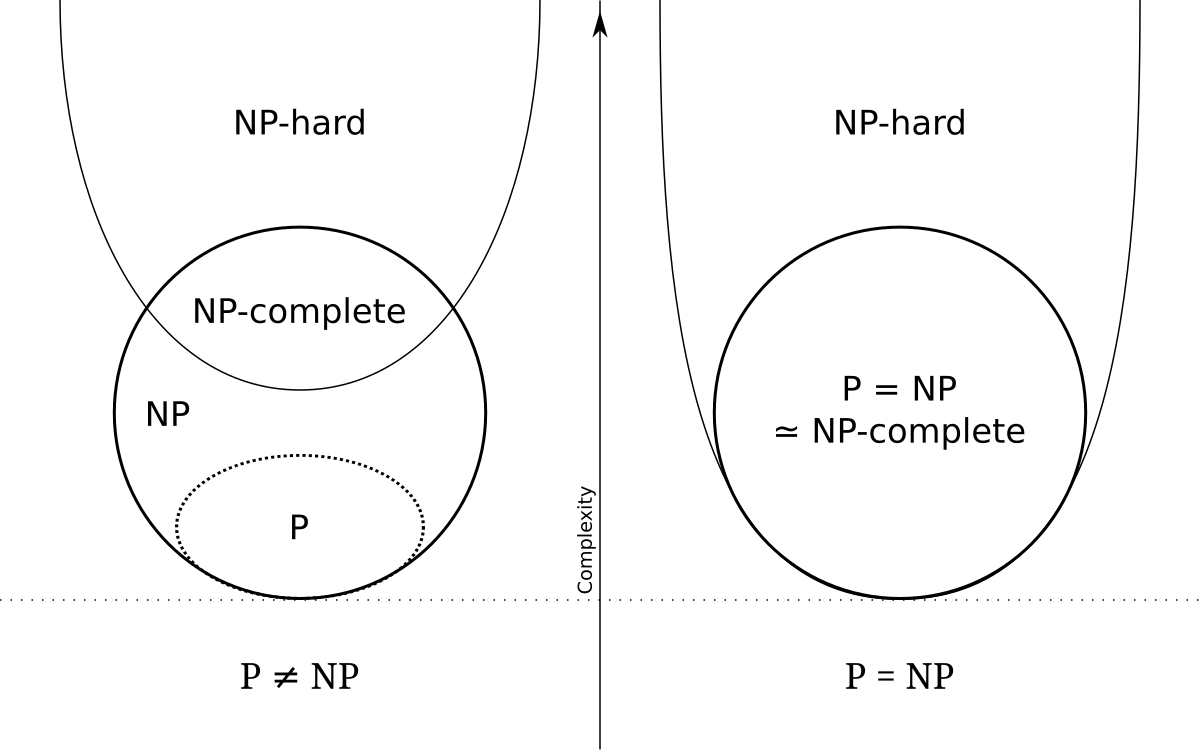
\includegraphics[
  width=\columnwidth,
  clip
]{nph.png}
}
In computational complexity theory, a decision problem \(H\) is called
\emph{NP-hard} if every problem \(L \in \mathrm{NP}\) can be reduced to \(H\)
via a polynomial-time many-one reduction. Formally,
\[
\forall L \in \mathrm{NP},\quad L \le_P H.
\]
This means that any polynomial-time algorithm capable of solving \(H\) can be
used (through the reduction) to solve every problem in NP. Hence, NP-hardness
is a \emph{hardness classification}: NP-hard problems are at least as difficult
as all NP problems.

\paragraph{NP-Hard vs.\ NP.}
A common point of confusion is that NP-hardness does not imply that a problem
is in NP. In fact, many NP-hard problems lie strictly outside NP, including:
\begin{itemize}
    \item PSPACE-complete problems (e.g.\ \textsc{TQBF}),
    \item EXPTIME-complete problems,
    \item recursively enumerable but undecidable problems (e.g.\ the Halting Problem).
\end{itemize}
These problems are NP-hard because every NP problem reduces to them, but they
are not in NP because they do not necessarily admit polynomial-time verifiers,
or may not even be decidable.

\paragraph{NP-Complete Problems.}
A problem is \emph{NP-complete} if it is both NP-hard and in NP:
\[
\mathrm{NPC} = \mathrm{NP} \cap \mathrm{NP\text{-}hard}.
\]
NP-complete problems are the ``hardest'' problems within NP: if any NP-complete
problem can be solved in polynomial time, then all NP problems can be solved in
polynomial time, implying \( \mathrm{P} = \mathrm{NP} \).

\begin{itemize}
    \item NP-complete problems lie in the intersection:
          \(\mathrm{NP} \cap \mathrm{NP\text{-}hard}\),
    \item NP-hard problems extend far beyond NP,
    \item NP-hardness is a hardness notion, not a membership class.
\end{itemize}

\paragraph{Summary.}
NP-hardness expresses that a problem is at least as hard as every problem in NP.
Such problems need not be in NP; they may lie outside polynomial-time verifiable
problems, or even outside decidable problems. NP-complete problems are exactly
the NP-hard problems that also lie inside NP.
\subsubsection{Karp Reductions: Propagation of Easiness and Hardness}

Given decision problems \(A\) and \(B\) with a Karp reduction \(A \le_P B\), we analyze which
complexity-class implications are valid. Recall that a Karp reduction allows us to transform
instances of \(A\) into instances of \(B\) in polynomial time while preserving membership:
\[
x \in A \iff f(x) \in B.
\]
This enables problem \(A\) to be solved using a solver for \(B\), and similarly enables
verification for \(A\) using a verifier for \(B\).

\paragraph{Incorrect Implications.}
Several answer choices incorrectly claim:
\begin{itemize}
    \item \(A \in P \Rightarrow B \in P\), or
    \item \(A \in NP \Rightarrow B \in NP\).
\end{itemize}
These are false because a reduction \(A \le_P B\) only shows how to solve or verify
\(A\) using an algorithm for \(B\); it does \emph{not} provide any method to solve or
verify \(B\) using an algorithm for \(A\). Thus, easiness does \emph{not} propagate from
\(A\) to \(B\) under a Karp reduction.

\paragraph{Correct Implications.}
The correct propagation rules under \(A \le_P B\) are:
\[
B \in P \;\Rightarrow\; A \in P,
\qquad
B \in NP \;\Rightarrow\; A \in NP.
\]
The first implication holds because a polynomial-time algorithm for \(B\), preceded by
the reduction \(f\), yields a polynomial-time algorithm for \(A\).
The second implication holds because an NP verifier for \(B\), preceded by \(f\),
yields a polynomial-time verifier for \(A\): the certificate for \(A\) can be reused
as the certificate for the reduced instance of \(B\).

These two implications correspond exactly to option (d), which is therefore the
correct answer.

\paragraph{Takeaway.}
A Karp reduction \(A \le_P B\) tells us:
\begin{itemize}
    \item \textbf{Easiness flows backward:} If \(B\) is easy (in \(P\) or \(NP\)), then \(A\) is easy.
    \item \textbf{Hardness flows forward:} If \(A\) is hard (e.g., NP-hard), then \(B\) is also hard.
\end{itemize}
Thus, under a Karp reduction, complexity never flows from \(A\) to \(B\): it always
flows in the opposite direction.

\subsection*{Graph Coloring: Algorithms \& Analysis}
\textit{Hint.} Anchor your reasoning with two easy bounds: the clique number $\omega(G)$ is a lower bound on $\chi(G)$, and a greedy pass in a good order gives a usable upper bound; a tight search prunes between them.

\paragraph{Problem.}
Given an undirected graph $G=(V,E)$, find the minimum number of colors $\chi(G)$ so that adjacent vertices receive different colors. Let $n=|V|$, $m=|E|$.

\paragraph{Basic Bounds (useful in analysis).}
\[
\omega(G)\ \le\ \chi(G)\ \le\ \Delta(G)+1,\qquad
\chi(G)\ \le\ d(G)+1
\]
where $\Delta$ is the max degree and $d(G)$ is the degeneracy (max core number). Brooks’ theorem sharpens the upper bound to $\chi(G)\le \Delta(G)$ except for cliques and odd cycles.

\paragraph{Greedy (Welsh–Powell) \& Degeneracy Orders.}
\textbf{Idea.} Order vertices (e.g., by nonincreasing degree or degeneracy order) and color each with the smallest available color.
\begin{itemize}
  \item \textbf{Complexity:} $O(n+m)$ with adjacency lists and bitsets per neighborhood.
  \item \textbf{Guarantee:} Uses at most $d(G)+1$ colors (optimal on chordal graphs with perfect elimination order).
\end{itemize}
\textbf{Pseudocode (Greedy).}
\begin{verbatim}
order = DegeneracyOrder(G)  // O(n+m)
for v in order:
  forbid = {color[u] : u in N(v) and colored(u)}
  color[v] = smallest nonnegative int not in forbid
\end{verbatim}

\paragraph{DSATUR Heuristic (Brélaz).}
\textbf{Idea.} Repeatedly pick the uncolored vertex with the highest \emph{saturation degree} (number of distinct neighbor colors); break ties by highest degree. Color it with the smallest feasible color.
\begin{itemize}
  \item \textbf{Why it works well:} Focuses early on constrained vertices, quickly increases the lower bound and often matches $\chi(G)$ in practice.
  \item \textbf{Complexity:} With efficient updates, $O(n^2)$–$O(n^2 \log n)$; each of $n$ steps inspects/updates neighbor color sets.
  \item \textbf{Bound use:} The number of colors used by DSATUR is an \emph{upper bound} $U$; the current max clique found gives a \emph{lower bound} $L$.
\end{itemize}
\textbf{Pseudocode (DSATUR).}
\begin{verbatim}
U = 0; for v: sat[v]=0, color[v]=-1
for step=1..n:
  v = argmax_{uncolored} (sat[v], degree[v])
  c = smallest color not used by N(v)
  color[v]=c; U = max(U, c+1)
  for u in N(v) with color[u]==-1: update sat[u]
\end{verbatim}

\paragraph{Exact Coloring: Branch-and-Bound on a Search Tree.}
\textbf{Idea.} Backtracking assigns colors to vertices one by one, pruning nodes where the partial assignment already forces $\ge U$ colors or conflicts. Tighten bounds using $L=\omega(G)$ (via clique search) and $U$ from fast coloring (DSATUR/greedy).
\begin{itemize}
  \item \textbf{State order:} Use DSATUR order dynamically to branch on the most constrained vertex.
  \item \textbf{Pruning rules:} (i) If current colors used $\ge U$, cut; (ii) if partial clique grows to $U$, no better solution below; (iii) color-class merging tests.
  \item \textbf{Complexity:} Exponential in the worst case (provably so), but very fast on many practical graphs due to strong pruning.
\end{itemize}
\textbf{Recurrence (conceptual).} Let $T(s)$ be expected nodes from state $s$; branching on $k$ feasible colors gives
\[
T(s)\ \le\ \sum_{i=1}^k T(s_i)\ +\ O(\deg(v)),
\]
with $k$ shrinking as bounds tighten; no closed form, but empirical growth is often much smaller than $k^n$.

\paragraph{Special Classes (Polynomial-Time).}
\begin{itemize}
  \item \textbf{Bipartite graphs:} $\chi=2$ iff no odd cycle. 2-color via BFS in $O(n+m)$.
  \item \textbf{Chordal graphs:} $\chi=\omega$; color optimally in $O(n+m)$ via perfect elimination order (MCS).
  \item \textbf{Interval/comparability/perfect graphs:} $\chi=\omega$; polynomial-time coloring using structure-specific orders.
  \item \textbf{Planar graphs:} $\chi\le 4$ (4CT). Linear-time 5-coloring; degeneracy $\le 5$ implies a trivial 6-coloring by greedy.
\end{itemize}
\textbf{Pseudocode (2-coloring BFS).}
\begin{verbatim}
for all v: color[v]=-1
for each component root r:
  color[r]=0; queue={r}
  while queue not empty:
    v=pop(); for u in N(v):
      if color[u]==-1: color[u]=1-color[v]; push(u)
      else if color[u]==color[v]: return "not bipartite"
return "2-coloring found"
\end{verbatim}

\paragraph{Approximation \& Hardness (high level).}
\begin{itemize}
  \item General graph coloring is NP-complete for $k\ge 3$; moreover, hard to approximate within $n^{1-\varepsilon}$ for any $\varepsilon>0$ in the worst case.
  \item Greedy gives a $(\Delta+1)$-coloring; degeneracy order yields $(d(G)+1)$ colors. On sparse graphs, $d(G)\ll \Delta$, giving better guarantees.
\end{itemize}

\paragraph{ILP / Set Cover Formulation (for exact solvers).}
\textbf{Set cover view:} Color classes are independent sets. Let $\mathcal{I}$ be the family of independent sets; choose a minimum subfamily covering $V$.
\[
\min \sum_{S\in \mathcal{I}} y_S \quad
\text{s.t. } \sum_{S\ni v} y_S \ge 1 \ \forall v,\ y_S\in\{0,1\}.
\]
Column generation adds violated independent sets via a maximum-weight independent set oracle.

\paragraph{Memory \& Engineering Notes.}
Use bitsets to represent color availability and adjacency (word-level parallelism), maintain tight upper bounds by reusing DSATUR in each node, and keep a running clique lower bound. For large sparse graphs, k-core ordering (degeneracy) yields small color counts and fast runtimes.

\paragraph{Takeaways.}
\begin{itemize}
  \item \textbf{Heuristics} (degeneracy, DSATUR) are fast and usually near-optimal.
  \item \textbf{Exact} B\&B becomes practical with strong $L/U$ bounds and informed branching.
  \item \textbf{Polynomial} algorithms exist for many structured classes; recognize them early.
  \item \textbf{Theory} is harsh on approximations in general, but structure-aware methods win in practice.
\end{itemize}

\subsection*{Tutorial 10 Questions}

\subsubsection*{Q1. Which of the following imply $P = NP$?}
\begin{enumerate}[(a)]
    \item There is a problem in P that is also NP-complete. [true]
    \item There is a problem in P that is also in NP.[$P \subseteq NP$, tautology]
    \item There is a problem in NP that is also NP-hard. [false. this only shows this problem is npc]
\end{enumerate}

\bigskip
\subsubsection*{Q2 \& Q3. Involving SUBSET-SUM}

Given a multiset $S$ of $n$ (usually non-negative) integers $\{S_1, S_2, \dots, S_n\}$ and an integer $W$, the \textbf{SUBSET-SUM} problem asks:

\[
\text{Does there exist a subset } I \subseteq \{1, 2, \dots, n\} \text{ such that } \sum_{i \in I} S_i = W?
\]

\paragraph{Example:}  
Given $n = 5$, $S = \{5, 1, 5, 1, 4\}$, and $W = 7$, then this is a YES-instance with certificates  
indices $\{0, 1, 3\}$ or values $\{5, 1, 1\}$ that sum to 7.

We want to prove that SUBSET-SUM is NP-complete, using the usual two-step proof.

\subsubsection*{Q2. Prove that SUBSET-SUM is in NP.}
Sum and equality check runs in $O(|S|)$
\subsubsection*{Q3. Prove that SUBSET-SUM is NP-hard.}
\begin{proof}
  Suppose a instance of 3-SAT, where there are $n$ variables, and $m$ clauses:\\
  $\forall x_i \in V, c_j \in C$, define the following numbers:
  \begin{itemize}
    \item $a_i = 10^{i + m} + \sum_{j: x_i \in c_j} 10^j$
    \item $b_i = 10^{i + m} + \sum_{j: \neg x_i \in c_j} 10^j$
    \item $p_j = 10^j$
    \item $q_j = 10^j$
  \end{itemize}
  \[W = \sum_{i=m}^{n+m-1} 10^i + 3\sum_{j=0}^{m-1} 10^j\]
  If in 3-SAT $\forall x_i \in V$ evaluates to true, select $a_i$, else select $b_i$;\\
  $\forall c_i \in C$ containing 1 true literal, select $q_i$;\\
  $\forall c_i \in C$ containing at most 2 true literal, select $p_i$;\\
  For an instance of 3-SAT to evaluate to YES, ie there exist an assignment of variables $V$ such that the CNF evaluates to true,
  the constructed SUBSET($\{a_i, b_i | i \in [1, n]\} \cup \{p_j, q_j | j \in [0, m-1]\}, W$) evaluates to YES.
\end{proof}
\subsubsection*{3-SAT(YES) $\implies$ Subsum(YES):}
for 3-SAT instance to be YES, following constraints need to be satisfied:
\begin{itemize}
  \item $\forall c_i \in C, \exists r \in \{1, 2, 3\}$ literals evaluates to true; 
  \item $\forall x_i \in V, x_i \lor \neg x_i$ 
\end{itemize}
Suppose $S_s = (S_{s1} \cup S_{s2})\subseteq S$ to be the subset thats has sum $W$:\\
$\forall x_i \in V,$ if $ x_i = true, $ $a_i \in S_{s1}$ else $b_i \in S_{s1} \implies \sum_{S_{s1}} = \sum_{i=m}^{n+m-1} 10^i + (k_i)\sum_{j=0}^{m-1}10^j$, where $k_i \in \{1, 2, 3\} $\\
$\forall c_i = (l_{i, 1} \lor l_{i, 2} \lor l_{i, 3})\in C,$, if $l_{i, 1} + l_{i, 2} + l_{i, 3} = 1$, $p_i \in S_{s2}$; if $l_{i, 1} + l_{i, 2} + l_{i, 3} = 2$, $q_i \in S_{s2} \implies 
\sum_{S_{s2}} = (3 - k)\sum_{j=0}^{m-1} 10^j$. \\
$\sum_{S_{s1} \cup S_{s2}} = \sum_{i=m}^{n+m-1} 10^i + 3\sum_{j=0}^{m-1} 10^j$

\subsubsection*{Subsum(YES) $\implies$ 3-SAT(YES)}
Suppose a YES instance of constructed subset sum, $S = \{a_i, b_i | i \in [1, n]\} \cup \{p_j, q_j | j \in [0, m-1]\}$, digit $0 \sim m - 1 = 3$, meaning:\\
$\forall i \in [1, n], a_i \oplus b_i \in S_s$, which accounts for digit $0 \sim m -1$ to be 1; \\
For a clause column $j\in\{0,\dots,m-1\}$. Let $k_j\in\{0,1,2,3\}$ be the number of true literals of $C_j$
under the assignment just defined; equivalently, $k_j$ is the number of chosen assignment items among
$\{a_i,b_i\}$ that contribute a $1$ in column $j$. The padding items $\{p_j,q_j\}$ can contribute at most
$2$ in column $j$. Since the target digit in column $j$ is $3$ and the total equals the target,
we must have $k_j\ge 1$. Therefore $C_j$ has at least one true literal.
\begin{align*}
  &\forall i \in [1, n], j \in [0, m-1], \\
  &(x_i \lor \neg x_i) \land ( \quad \quad \quad\quad\quad\quad\quad\quad\quad\quad\quad\quad\quad\quad\quad\quad\quad\quad\quad\quad\quad\quad\quad\quad\quad\quad \text{ MSB } 0 \sim n\\
  &((\sum_{r=1}^{3} l_{j, i, r} = 2) \land (\sum_{r = 1}^{3}((l_{j, i, r} = x_i) \land x_i) \lor ((l_{j, i, r} = \neg x_i) \land \neg x_i)) = 1) \lor \quad \text{LSB } 0 \sim m \text{ Case: 2 true literals}\\
  &((\sum_{r=1}^{3} l_{j, i, r} = 1) \land (\sum_{r = 1}^{3}((l_{j, i, r} = x_i) \land x_i) \lor ((l_{j, i, r} = \neg x_i) \land \neg x_i)) = 2) \lor \quad \text{LSB } 0 \sim m \text{ Case: 1 true literals}\\
  &((\sum_{r=1}^{3} l_{j, i, r} = 3) \land (\sum_{r = 1}^{3}((l_{j, i, r} = x_i) \land x_i) \lor ((l_{j, i, r} = \neg x_i) \land \neg x_i)) = 3) \lor \quad \text{LSB } 0 \sim m \text{ Case: 3 true literals}\\
  &)\\
\end{align*}

\bigskip







\subsubsection*{Q4 \& Q5. Involving FIND-FAMILY}

\paragraph{Definitions:}
\begin{itemize}
    \item An undirected bipartite graph $G = (L \cup R, E)$ has two disjoint vertex sets $L$ and $R$, where each edge connects one vertex in $L$ and one in $R$.
    \item Two vertices $u, v \in L$ are called \textbf{siblings} if there exists a vertex $r \in R$ such that both edges $(u, r)$ and $(r, v)$ are present.
    \item A subset $F \subseteq L$ is said to be a \textbf{family} if for all distinct $u, v \in F$, $u$ and $v$ are siblings.
\end{itemize}

\paragraph{Decision problem: FIND-FAMILY}
\[
\text{Given } G = (L \cup R, E), \text{ is there a family of size } \geq k?
\]

\begin{figure}[h]
    \centering
    \caption{Example bipartite graph with $L = \{0, 2, 4\}$ and $R = \{1, 3\}$.  
    Here, 0 and 2 are siblings, 2 and 4 are siblings, but $\{0, 2, 4\}$ is not a family since 0 and 4 are not siblings.}
\end{figure}

We want to prove that FIND-FAMILY is NP-complete, using the usual two-step proof.

\subsubsection*{Q4. Prove that FIND-FAMILY is in NP.}

\subsubsection*{Q5. Prove that FIND-FAMILY is NP-hard.}
\subsubsection*{CLIQUE $\leq_P$ FIND-FAMILY}
\begin{proof}
  \subsubsection*{Constrction}
  From an instance of CLIQUE($G = (V, E), k$), construct an instance of FIND-FAMILY($G' = (V', E'), k$), 
  where $V'' = V' \cup U, V' = V, U = \{u_e | e \in E\}$,
  $E' = \{(v, u_e),  (u_e, v')| v, v' \in V, (v, v') \in E\}$. 
  \subsubsection*{CLIQUE(YES) $\implies$ FIND-FAMILY(YES)}
  Suppose a YES instance of CLIQUE, $\exists S\subseteq V, |S| \geq k, \forall v, v' \in S, v \neq v'\exists 
  v \times v' \in E$. In the construction, $\forall v \in S$ in CLIQUE(YES), 
  $\exists! v' \in F \subseteq V', \exists! u \in U, (v', u) \in E'$,$F$ is a family with size $k$.
  \subsubsection*{FIND-FAMILY(YES) $\implies$ CLIQUE(YES)}
  Suppose a YES instance of constructed FIND-FAMILY, $\exists S \subseteq V', |S| = k, \exists! u \in U, (v', u) \in E'$, consider the
  construction as a function $f: (v, v') \mapsto \{(v, u) \cup (u, v')\}$
\end{proof}
\newpage
\section{Common NPC proofs}
\subsection{Reduction from \textsc{Circuit-SAT} to \textsc{SAT} (NP-Completeness of SAT)}

In this subsection we present a detailed polynomial-time reduction from the
\textsc{Circuit-SAT} problem to the \textsc{SAT} problem.  Together with the
observation that \textsc{SAT} is in NP, this establishes that \textsc{SAT} is
NP-complete.  The key idea behind the reduction is to encode the behaviour of
each gate in a Boolean circuit using a small collection of CNF clauses, thus
constructing a CNF formula whose satisfying assignments correspond exactly to the
consistent truth assignments of the circuit.

\paragraph{Conceptual Note.}
A Boolean circuit is simply a directed acyclic graph with gates
(\textsc{AND}, \textsc{OR}, \textsc{NOT}) as internal nodes and Boolean inputs
as sources.  A circuit evaluates deterministically: once the inputs are
assigned, the value of every internal wire is forced by the gate semantics.
\textbf{The reduction relies on the following idea:}
\begin{quote}
    \emph{Introduce one propositional variable for every wire in the circuit, and
    enforce the correct behaviour of each gate using a constant-size CNF
    formula.}
\end{quote}
If all gate constraints are satisfied and the output wire is forced to be $1$,
we have precisely captured the notion of a ``valid evaluation'' of the circuit.

\subsubsection*{Encoding Gates in CNF}

Let $u, v, w$ denote propositional variables corresponding to the input and
output wires of a gate.  We now express each gate relationship using CNF
constraints.  The preservation of the gate semantics is achieved by encoding the
logical equivalence
\[
    w \leftrightarrow \text{Gate}(u,v)
\]
as a conjunction of implications.

\paragraph{AND Gate.}
For a gate $w = u \land v$, we enforce:
\[
\begin{aligned}
w \Rightarrow u &\quad\Rightarrow\quad (\neg w \lor u),\\
w \Rightarrow v &\quad\Rightarrow\quad (\neg w \lor v),\\
u \land v \Rightarrow w &\quad\Rightarrow\quad (\neg u \lor \neg v \lor w).
\end{aligned}
\]
Thus the CNF block for an \textsc{AND} gate is:
\[
(\neg w \lor u)\,\land\,(\neg w \lor v)\,\land\,(\neg u \lor \neg v \lor w).
\]

\paragraph{OR Gate.}
For a gate $w = u \lor v$:
\[
\begin{aligned}
w \Rightarrow (u \lor v) &\quad\Rightarrow\quad (\neg w \lor u \lor v),\\
u \Rightarrow w &\quad\Rightarrow\quad (\neg u \lor w),\\
v \Rightarrow w &\quad\Rightarrow\quad (\neg v \lor w).
\end{aligned}
\]
Thus the CNF block is:
\[
(\neg w \lor u \lor v)\,\land\,(\neg u \lor w)\,\land\,(\neg v \lor w).
\]

\paragraph{NOT Gate.}
For a gate $w = \neg u$:
\[
\begin{aligned}
w \Rightarrow \neg u &\quad\Rightarrow\quad (\neg w \lor \neg u),\\
\neg u \Rightarrow w &\quad\Rightarrow\quad (u \lor w).
\end{aligned}
\]
So the CNF block is:
\[
(\neg w \lor \neg u)\,\land\,(u \lor w).
\]

\paragraph{Conceptual Note.}
Each of the above CNF blocks admits exactly the satisfying assignments consistent
with the intended gate semantics.  No illegal combination of wire values can
satisfy all clauses of the block.

\subsubsection*{Constructing the Formula}

Let $C$ be a Boolean circuit with input wires $x_1,\dots,x_n$, internal wires
$y_1,\dots,y_m$, and a single output wire $z$.  We define a CNF formula
$\varphi_C$ as follows:

\begin{enumerate}
    \item \textbf{Variables.}  
    The variables of $\varphi_C$ are all wire variables:
    \[
        \{x_1,\dots,x_n, y_1,\dots,y_m, z\}.
    \]
    \item \textbf{Gate Constraints.}  
    For every gate in $C$ with input wires $(u,v)$ and output $w$, append the
    CNF clauses corresponding to its type (AND/OR/NOT) as described above.
    Each gate contributes at most $3$ clauses of size at most $3$.
    \item \textbf{Output Constraint.}
    Enforce that the final output wire must evaluate to $1$:
    \[
        (z).
    \]
\end{enumerate}

The resulting formula $\varphi_C$ is clearly in CNF, and its size is linear in
the number of gates of $C$.

\subsubsection*{Correctness of the Reduction}

We prove that for every Boolean circuit $C$,
\[
    C \text{ is satisfiable} \iff \varphi_C \text{ is satisfiable}.
\]

\paragraph{($\Rightarrow$) If the circuit is satisfiable.}

Suppose some assignment to the input wires makes the circuit output $1$.
Evaluating the circuit gate-by-gate yields unique values for all internal and
output wires.  Let $\beta$ denote this full assignment to all wire variables.

Each gate constraint added to $\varphi_C$ is satisfied by $\beta$ because
$\beta$ assigns the correct output to each gate given its inputs.  Furthermore,
$\beta(z)=1$, so the clause $(z)$ is satisfied.  Hence $\varphi_C$ is satisfiable.

\paragraph{($\Leftarrow$) If the formula is satisfiable.}

Let $\beta$ be any satisfying assignment of $\varphi_C$.  In particular,
$\beta$ satisfies all constraints encoding the behaviour of each gate.  Since
each CNF block admits only the assignments consistent with the truth table of
the corresponding gate, the wire assignments under $\beta$ force each gate to
operate correctly.

Thus, if we restrict $\beta$ to the input wires $x_1,\dots,x_n$ and evaluate the
circuit in the usual manner, the induced gate evaluations must agree with
$\beta$ on every internal wire and on the output wire $z$.  Because the final
clause $(z)$ is satisfied, $\beta(z)=1$, and hence the circuit outputs~$1$ under
that input assignment.  Therefore, $C$ is satisfiable.

\subsubsection*{Polynomial-Time Complexity}

The construction of $\varphi_C$ involves a single pass over all gates of the
circuit, adding a constant number of constant-size clauses for each.  Hence
$f(C)=\varphi_C$ is produced in time $\mathcal{O}(|C|)$, i.e., polynomial in the
size of the circuit.

\subsubsection*{Conclusion}

Since \textsc{Circuit-SAT} is NP-complete and
\[
    \textsc{Circuit-SAT} \le_p \textsc{SAT},
\]
it follows by definition that \textsc{SAT} is NP-hard.  Together with the fact
that \textsc{SAT} is in NP, we conclude that \textsc{SAT} is NP-complete.
\subsection{Reduction from \textsc{3-SAT} to \textsc{NAE-3-SAT}$^+$}

In this subsection we present a polynomial-time reduction from \textsc{3-SAT} to
the \textsc{Not-All-Equal 3-SAT} problem with only positive literals, denoted
\textsc{NAE-3-SAT}$^+$.  In \textsc{NAE-3-SAT}$^+$ we are given clauses of the
form $(a,b,c)$ where $a,b,c$ are positive Boolean variables, and a clause is
satisfied under an assignment if \emph{not all three literals have the same
truth value}.  That is, both $(0,0,0)$ and $(1,1,1)$ are forbidden; all other
assignments satisfy the clause.

\paragraph{Conceptual Note.}
A clause in ordinary 3-SAT is satisfied whenever \emph{at least one literal is
true}.  In contrast, a clause in NAE-3-SAT is satisfied whenever the three
literals are \emph{not} all equal.  This is a symmetry-based notion:
\[
(0,0,1), (0,1,0), (1,0,0), (1,1,0), (1,0,1), (0,1,1)\quad\text{are all acceptable}.
\]
Since \textsc{NAE-3-SAT}$^+$ forbids negations, achieving the reduction requires
introducing a reference variable representing a ``truth baseline'' and
encodings that simulate negation by separating variables from this baseline.

\subsubsection*{Construction of the Reduction}

Let an instance of \textsc{3-SAT} be a CNF formula
\[
\varphi = \bigwedge_{i=1}^m (l_{i1} \lor l_{i2} \lor l_{i3}),
\]
where each $l_{ij}$ is either a positive literal $x$ or a negative literal
$\neg x$.  We construct an instance $\psi$ of \textsc{NAE-3-SAT}$^+$ as follows.

\paragraph{Step 1: Introduce a global reference variable.}

Add a fresh variable $t$ (the ``truth baseline'').  Intuitively, $t$ will serve
as the point against which all literal truth values are compared.  A positive
literal $x$ will be interpreted as ``$x$ differs from $t$ in the NAE sense''
(i.e., the clause is satisfied when $x$ is not equal to $t$), while a negated
literal $\neg x$ will be simulated by the requirement that $x$ \emph{agrees}
with~$t$.

\paragraph{Step 2: Simulating literals.}

For each literal $l$ appearing in the 3-SAT instance, we associate the following
pair of NAE conditions:
\begin{itemize}
    \item If $l = x$ (a positive literal), we will use $x$ directly in clauses
    together with $t$.
    \item If $l = \neg x$, we simulate negation by introducing a fresh variable
    $x'$ and adding the NAE constraint
    \[
    \operatorname{NAE}(x, x', t),
    \]
    enforcing the parity condition: exactly one of $x$ and $x'$ equals $t$.  
    In effect, $x'$ becomes an NAE-encoding of ``$\neg x$’’.
\end{itemize}

\paragraph{Conceptual Note.}
The constraint $\operatorname{NAE}(x,x',t)$ enforces:
\[
x = t \iff x' \neq t, \qquad
x \neq t \iff x' = t.
\]
Thus $x'$ functions as a negated version of $x$ relative to the baseline $t$.

\paragraph{Step 3: Converting each clause.}

Given a 3-SAT clause $(l_1 \lor l_2 \lor l_3)$, we create the NAE clause
\[
\operatorname{NAE}(l_1^*, l_2^*, l_3^*),
\]
where each $l_i^*$ is the corresponding NAE variable:
\begin{itemize}
    \item If $l_i = x$, then $l_i^* = x$.
    \item If $l_i = \neg x$, then $l_i^* = x'$ (defined via the relation
    $\operatorname{NAE}(x,x',t)$).
\end{itemize}
Since all NAE clauses use only positive variables $x, x', t$, the instance is
indeed a valid \textsc{NAE-3-SAT}$^+$ formula.

\subsubsection*{Correctness of the Reduction}

We now argue that
\[
\varphi \text{ is satisfiable} \iff \psi \text{ is NAE-satisfiable}.
\]

\paragraph{($\Rightarrow$) If $\varphi$ is satisfiable.}

Let $\alpha$ be a satisfying assignment for $\varphi$.  Construct an assignment
$\beta$ for the variables of $\psi$ as follows:
\begin{enumerate}
    \item Choose $t = 0$ (arbitrary; the construction is symmetric).
    \item Set $\beta(x) = \alpha(x)$ for all original variables.
    \item For each $x'$ representing $\neg x$, set
    \[
        \beta(x') = 1 - \alpha(x),
    \]
    ensuring $\operatorname{NAE}(x,x',t)$ is satisfied.
\end{enumerate}

We claim that each NAE clause $\operatorname{NAE}(l_1^*,l_2^*,l_3^*)$
originating from the 3-SAT clause $(l_1 \lor l_2 \lor l_3)$ is satisfied under
$\beta$.  Indeed, since $(l_1 \lor l_2 \lor l_3)$ is true under $\alpha$,
exactly one of the following holds:
\begin{itemize}
    \item Some positive $x$ among the three is $1$, hence differs from $t$.
    \item Some negative $\neg x$ is true, so $x = 0$ and therefore $\beta(x') =
    1$, differing from $t$.
\end{itemize}
Thus among the triple $(l_1^*, l_2^*, l_3^*)$ at least one variable differs
from $t$, meaning the triple is not monochromatic.  Therefore the NAE clause is
satisfied.  Hence $\psi$ is NAE-satisfiable.

\paragraph{($\Leftarrow$) If $\psi$ is NAE-satisfiable.}

Let $\beta$ satisfy $\psi$.  We first normalize the assignment by possibly
flipping all variables:
\begin{quote}
    If necessary, replace every value $b$ by $1-b$ so that $\beta(t)=0$.
\end{quote}
This preserves satisfaction of all NAE clauses (NAE is invariant under global
complementing).

For each original variable $x$ we set
\[
    \alpha(x) = \beta(x).
\]
For each negated literal $\neg x$ we examine the constraint
$\operatorname{NAE}(x,x',t)$.  Since $\beta(t)=0$, exactly one of $x$ and $x'$
equals $1$:
\[
\beta(x') = 1 \iff \beta(x) = 0.
\]
Thus a clause $(l_1 \lor l_2 \lor l_3)$ from $\varphi$ is satisfied by $\alpha$:
in its corresponding NAE clause, at least one variable differs from $t=0$, hence
is equal to $1$, so its source literal in the 3-SAT clause is true.  Therefore
$\alpha$ satisfies $\varphi$.

\subsubsection*{Polynomial-Time Complexity}

The reduction creates one fresh variable $x'$ for each negated literal and a
constant number of NAE clauses per original clause.  The total size of $\psi$ is
thus linear in the size of $\varphi$, and the construction is computable in
$\mathcal{O}(|\varphi|)$ time.

\subsubsection*{Conclusion}

We have established a polynomial-time reduction
\[
    \textsc{3-SAT} \le_p \textsc{NAE-3-SAT}^+.
\]
Since \textsc{3-SAT} is NP-complete, it follows that \textsc{NAE-3-SAT}$^+$ is
NP-hard.  As NAE-satisfiability can be checked using a polynomial-time verifier,
\textsc{NAE-3-SAT}$^+$ is NP-complete.
\subsubsection*{Extension: From \textsc{3-SAT} to General \textsc{NAE-3-SAT}}

In the previous subsection we reduced \textsc{3-SAT} to the positive–literal
variant \textsc{NAE-3-SAT}$^+$, where clauses must contain only unnegated
variables.  This required the introduction of a global baseline variable $t$ and
auxiliary variables $x'$ to simulate negation in an NAE context.

When the target problem is the standard version of \textsc{NAE-3-SAT},
\emph{which permits negated literals}, the reduction becomes much simpler.
Indeed, the Not-All-Equal relation already handles negation naturally, because:
\[
\operatorname{NAE}(u,v,w) \quad\text{is symmetric under complementing any
subset of its input variables.}
\]
Thus, the key complexity of the $+$ version disappears.

\paragraph{Key Insight.}
For ordinary NAE-3-SAT, a clause such as
\[
(l_1 \lor l_2 \lor l_3)
\]
can be translated directly to an NAE clause
\[
\operatorname{NAE}(l_1, l_2, l_3, t),
\]
where $t$ is a single new variable included in every clause.
The role of $t$ is to “break” the monochromatic all-0 assignment, yet because
negations are allowed, we do not need $x'$ variables: negated literals may be
used directly in the NAE clause.

\paragraph{Construction.}

Given a 3-SAT instance
\[
\varphi = \bigwedge_{i=1}^m (l_{i1} \lor l_{i2} \lor l_{i3}),
\]
introduce one new variable $t$.  
For each clause $(l_{i1},l_{i2},l_{i3})$ produce the NAE clause
\[
\operatorname{NAE}(l_{i1}, l_{i2}, l_{i3}, t).
\]

This is legal in NAE-3-SAT because negated literals are allowed.

\paragraph{Why this works.}
Observe the following facts:

\begin{enumerate}
    \item The NAE clause 
    \[
        \operatorname{NAE}(l_{i1},l_{i2},l_{i3},t)
    \]
    forbids both all-0 and all-1 assignments.

    \item If at least one of $l_{i1},l_{i2},l_{i3}$ is true, then by choosing
    $t=0$ the clause is satisfied.

    \item If all three $l_{ij}$ are false, then the clause becomes
    $\operatorname{NAE}(0,0,0,t)$, which requires $t=1$.
    But because $t$ appears in \emph{every} clause, some other clause that has a
    true literal would enforce $t=0$, creating a contradiction.

    Hence no satisfying NAE assignment can allow all three literals of a clause
    to be false.
\end{enumerate}

Consequently, each clause behaves exactly like an OR-clause in the original
formula.

\paragraph{Correctness.}

\textbf{($\Rightarrow$)} If $\varphi$ is satisfiable, fix $t = 0$.  
Each clause has at least one true literal, so no clause becomes monochromatic.
Therefore all NAE clauses are satisfied.

\textbf{($\Leftarrow$)} If the NAE formula is satisfiable, $t$ must have a fixed
value across all clauses.  
If a clause had all three literals false, that clause would force $t=1$, but
any clause with a true literal forces $t=0$, contradicting satisfiability.  
Therefore no clause has all literals false, meaning every clause has at least
one true literal — exactly the 3-SAT condition.

\paragraph{Comparison to the \textsc{NAE-3-SAT}$^+$ Reduction.}

The positive-literal version required:
\begin{itemize}
    \item a baseline variable $t$,
    \item an auxiliary variable $x'$ for each negated literal,
    \item an NAE constraint $\operatorname{NAE}(x,x',t)$ per negation,
    \item and NAE clauses using only positive literals.
\end{itemize}

In general NAE-3-SAT:
\begin{itemize}
    \item negated literals are allowed directly,
    \item the parity gadget $\operatorname{NAE}(x,x',t)$ disappears,
    \item each 3-SAT clause becomes a \emph{single} 4-variable NAE clause,
    \item and the entire reduction requires only one new variable $t$.
\end{itemize}

Thus the standard NAE-3-SAT reduction is significantly simpler and more compact
than the positive-literal version.


\subsection{Reduction from \textsc{3-SAT} to \textsc{0-1-Linear-SAT}}

We now present a polynomial-time reduction from \textsc{3-SAT} to a linear
satisfiability problem over $\{0,1\}$-valued variables, which we call
\textsc{0-1-Linear-SAT}.  An instance of \textsc{0-1-Linear-SAT} consists of:
\begin{itemize}
    \item variables $x_1,\dots,x_n$ with domain $\{0,1\}$, and
    \item a finite set of linear inequalities of the form
    \[
        a_{1}x_1 + \dots + a_{n}x_n \;\ge\; b,
    \]
    where $a_i,b$ are integers.
\end{itemize}
The question is whether there exists an assignment $x \in \{0,1\}^n$
satisfying all inequalities simultaneously.

\paragraph{Conceptual Note.}
A 3-SAT clause $(\ell_1 \lor \ell_2 \lor \ell_3)$ is satisfied iff \emph{at least
one} of the three literals is true.  For $\{0,1\}$-valued variables, “at least
one is true” is naturally expressed as a \emph{sum inequality}:
\[
\ell_1 + \ell_2 + \ell_3 \;\ge\; 1,
\]
provided we interpret each literal as a linear expression:
\[
\ell = x_j \text{ if it is positive}, \qquad
\ell = 1 - x_j \text{ if it is negative}.
\]
This is the key idea behind the reduction.

\subsubsection*{Construction of the Reduction}

Let a 3-SAT instance be given as a CNF formula
\[
\varphi = \bigwedge_{i=1}^m (l_{i1} \lor l_{i2} \lor l_{i3}),
\]
over variables $X = \{x_1,\dots,x_n\}$, where each $l_{ij}$ is either $x_k$ or
$\neg x_k$ for some $k$.

We construct an instance of \textsc{0-1-Linear-SAT} as follows.

\paragraph{Variables.}
For each Boolean variable $x_j$ in $\varphi$, we create a 0–1 variable (with the
same name) $x_j \in \{0,1\}$.  We interpret $x_j = 1$ as ``true'' and
$x_j = 0$ as ``false''.

\paragraph{Literal Encoding.}
For each literal $l$ we define a corresponding linear expression $E(l)$:
\[
E(l) \;=\;
\begin{cases}
x_j, & \text{if } l = x_j,\\
1 - x_j, & \text{if } l = \neg x_j.
\end{cases}
\]
Note that if $x_j \in \{0,1\}$, then $E(l) \in \{0,1\}$ and
\[
E(l) = 1 \iff l \text{ is true under the Boolean assignment}.
\]

\paragraph{Clause Encoding.}
For each clause $C_i = (l_{i1} \lor l_{i2} \lor l_{i3})$ in $\varphi$, we add
the inequality
\[
E(l_{i1}) + E(l_{i2}) + E(l_{i3}) \;\ge\; 1.
\]
Intuitively, at least one of the three literals must evaluate to $1$ (true), so
the sum must be at least $1$.

\paragraph{Resulting System.}
The \textsc{0-1-Linear-SAT} instance $\mathcal{L}_\varphi$ consists of:
\begin{itemize}
    \item variables $x_1,\dots,x_n \in \{0,1\}$, and
    \item the $m$ inequalities
    \[
        E(l_{i1}) + E(l_{i2}) + E(l_{i3}) \;\ge\; 1, \quad i = 1,\dots,m.
    \]
\end{itemize}

\subsubsection*{Correctness of the Reduction}

We prove that $\varphi$ is satisfiable iff $\mathcal{L}_\varphi$ is satisfiable.

\paragraph{($\Rightarrow$) If $\varphi$ is satisfiable.}

Assume there exists a Boolean assignment
\[
\alpha : \{x_1,\dots,x_n\} \to \{0,1\}
\]
that satisfies $\varphi$.  Define a 0–1 vector
\[
x_j = \alpha(x_j), \quad j = 1,\dots,n.
\]

Consider any clause $C_i = (l_{i1} \lor l_{i2} \lor l_{i3})$.  
Because $\alpha$ satisfies $\varphi$, we must have
\[
\alpha(l_{i1}) = 1 \quad \text{or} \quad
\alpha(l_{i2}) = 1 \quad \text{or} \quad
\alpha(l_{i3}) = 1.
\]
By construction of $E(l)$ and the fact that $x_j = \alpha(x_j)$, we have
\[
E(l_{ij}) = 1 \iff l_{ij} \text{ is true under } \alpha.
\]
Therefore, for each clause,
\[
E(l_{i1}) + E(l_{i2}) + E(l_{i3}) \;\ge\; 1.
\]
So the assignment $(x_1,\dots,x_n)$ satisfies all the inequalities in
$\mathcal{L}_\varphi$, and hence $\mathcal{L}_\varphi$ is feasible.

\paragraph{($\Leftarrow$) If $\mathcal{L}_\varphi$ is satisfiable.}

Conversely, suppose there exists $x \in \{0,1\}^n$ satisfying all inequalities
of $\mathcal{L}_\varphi$.  Define a Boolean assignment
\[
\alpha(x_j) = x_j, \quad j = 1,\dots,n.
\]

For any clause $C_i = (l_{i1} \lor l_{i2} \lor l_{i3})$, we know that
\[
E(l_{i1}) + E(l_{i2}) + E(l_{i3}) \;\ge\; 1,
\]
and each $E(l_{ij}) \in \{0,1\}$.  Hence, at least one of the terms
$E(l_{i1}), E(l_{i2}), E(l_{i3})$ is equal to $1$.

But by construction,
\[
E(l_{ij}) = 1 \iff l_{ij} \text{ is true under } \alpha.
\]
Thus, for each clause $C_i$, at least one literal $l_{ij}$ is true under
$\alpha$, so $C_i$ is satisfied.  Since this holds for all clauses, $\alpha$
satisfies $\varphi$.

\subsubsection*{Polynomial-Time Complexity}

The reduction introduces no new variables beyond the original $x_1,\dots,x_n$,
and creates exactly one inequality per clause, with at most three nonzero
coefficients and a constant-size right-hand side.  Therefore, the size of
$\mathcal{L}_\varphi$ is linear in the size of $\varphi$, and the construction
clearly runs in time $\mathcal{O}(|\varphi|)$.

\subsubsection*{Conclusion}

We have defined a polynomial-time reduction
\[
    \textsc{3-SAT} \le_p \textsc{0-1-Linear-SAT},
\]
by encoding each 3-CNF clause as a linear inequality over $\{0,1\}$-valued
variables.  Since \textsc{3-SAT} is NP-complete, this implies that
\textsc{0-1-Linear-SAT} is NP-hard.  Because a candidate 0–1 vector can be
verified in polynomial time, \textsc{0-1-Linear-SAT} is NP-complete.
\subsection{Reduction from \textsc{3-SAT} to \textsc{Exact-1 3-SAT}}

We present a polynomial-time reduction from \textsc{3-SAT} to the
\textsc{Exact-1 3-SAT} (also called ``1-in-3-SAT'') problem.  In
\textsc{Exact-1 3-SAT} each clause consists of exactly three literals, and a
clause is satisfied if and only if \emph{exactly one} of the three literals is
true.  Unlike ordinary 3-SAT, where a clause is satisfied if at least one
literal is true, the exact-1 constraint enforces a precise combinatorial
structure.

\paragraph{Conceptual Note.}
A 3-SAT clause 
\[
(l_1 \lor l_2 \lor l_3)
\]
admits many satisfying assignments.  In contrast, the
\textsc{Exact-1} clause $(a,b,c)$ restricts to exactly three allowed assignments:
\[
(1,0,0),\ (0,1,0),\ (0,0,1).
\]
To simulate an OR-clause using exact-1 constraints, we introduce fresh
``selector’’ variables that distribute the truth value among multiple
exact-1 clauses.  The key idea is to enforce the logical condition:
\[
l_1 \lor l_2 \lor l_3 \quad\text{is true} 
\quad\Longleftrightarrow\quad
\text{at least one of } l_1, l_2, l_3 \text{ is true}.
\]
This will be encoded through a gadget ensuring exactly one literal among an
expanded set is chosen while allowing us to recover the intended OR-semantics.

\subsubsection*{Construction of the Reduction}

Let the 3-SAT instance be
\[
\varphi = \bigwedge_{i=1}^m (l_{i1} \lor l_{i2} \lor l_{i3}),
\]
where each literal $l_{ij}$ is either $x_k$ or $\neg x_k$.

For each clause $C_i=(l_{i1},l_{i2},l_{i3})$ we construct a constant-size
gadget using fresh variables.  The construction below is the classical
Schaefer gadget.

\paragraph{Step 1: Literal Variables.}

We keep all original variables.  Negated literals $\neg x$ are treated
directly as Boolean negations inside clauses; no expansion is needed.

\paragraph{Step 2: Introduce Clause Selector Variables.}

For each clause $C_i$, create a new auxiliary variable $s_i$.
Intuitively, $s_i$ acts as a ``switch’’ selecting which literal is made true
within the exact-1 enforcement.

\paragraph{Step 3: Replace Each Clause with Three Exact-1 Clauses.}

For the clause $(l_{i1} \lor l_{i2} \lor l_{i3})$, introduce the following
three exact-1-clauses:
\[
\operatorname{X1}(l_{i1}, s_i, a_i), \qquad
\operatorname{X1}(l_{i2}, s_i, b_i), \qquad
\operatorname{X1}(l_{i3}, s_i, c_i),
\]
where $a_i,b_i,c_i$ are fresh auxiliary variables.

Here $\operatorname{X1}(u,v,w)$ denotes a clause of the form
``\emph{exactly one of $u,v,w$ is true}.’’

\paragraph{Intuition.}
The selector variable $s_i$ appears in all three clauses.  If the original
clause $(l_{i1},l_{i2},l_{i3})$ is to be satisfied, then at least one
literal must be true.  The exact-1 constraints ensure that:

- If one of the literals $l_{i1},l_{i2},l_{i3}$ is true, that literal will be
paired with $s_i$ and one auxiliary variable in such a way that exactly one is
true per clause.

- If none of the literals is true, then $s_i$ would be forced to satisfy all
three clauses alone, which is impossible because $s_i$ appears identically in
all three exact-1 clauses.

Thus the gadget forces at least one literal of the original clause to be true.

\subsubsection*{Correctness of the Reduction}

We now prove:
\[
\varphi \text{ is satisfiable} \iff \psi \text{ is Exact-1 satisfiable}.
\]

\paragraph{($\Rightarrow$) If $\varphi$ is satisfiable.}

Assume a Boolean assignment $\alpha$ satisfies each clause
$(l_{i1},l_{i2},l_{i3})$.  
Fix a clause $C_i$ and choose one literal $l_{ij}$ that is true under $\alpha$.
Set:

- $s_i = 0$,
- $a_i,b_i,c_i$ so that exactly the true literal is chosen in each clause.

Then each of:
\[
\operatorname{X1}(l_{i1}, s_i, a_i),\ 
\operatorname{X1}(l_{i2}, s_i, b_i),\ 
\operatorname{X1}(l_{i3}, s_i, c_i)
\]
is satisfied: one literal (the true one) becomes the ``1’’ in its clause, and
the auxiliary variable handles the remaining exact-1 structure.  
Doing this independently for each clause produces an assignment satisfying all
exact-1 constraints.

\paragraph{($\Leftarrow$) If $\psi$ is Exact-1 satisfiable.}

Suppose $\beta$ satisfies all exact-1 clauses.  
Fix a clause gadget corresponding to $C_i$.  The three exact-1 clauses share
$s_i$.  
If all three original literals $l_{i1},l_{i2},l_{i3}$ were false under the
assignment to original variables, then $s_i$ would have to be the unique true
literal in all three clauses simultaneously.  But this is impossible: $s_i$
cannot satisfy three different exact-1 constraints where the other two literals
in each clause differ.

Therefore, at least one of the three literals $l_{i1},l_{i2},l_{i3}$ must be
true under the restriction of $\beta$ to the original variables.  Hence the
original 3-SAT clause is satisfied.

Thus the induced assignment on $\{x_1,\dots,x_n\}$ satisfies all clauses of
$\varphi$.

\subsubsection*{Polynomial-Time Complexity}

The reduction introduces a constant number of new variables and exactly three
exact-1 clauses per original clause.  Therefore the size of $\psi$ is linear in
the size of the input $\varphi$, and the construction clearly runs in time
$\mathcal{O}(|\varphi|)$.

\subsubsection*{Conclusion}

We have established a polynomial-time reduction:
\[
    \textsc{3-SAT} \le_p \textsc{Exact-1 3-SAT}.
\]
Since \textsc{3-SAT} is NP-complete and exact-1-satisfiability is verifiable in
polynomial time, \textsc{Exact-1 3-SAT} is NP-complete.



\subsection{Reduction from \textsc{3-SAT} to Group Interval Scheduling (Group Size $\ge 3$)}

In the \emph{Group Interval Scheduling} decision problem (GIS), the input is:
\begin{itemize}
    \item a set of groups $G_1,\dots,G_m$, each group $G_i$ containing several
          intervals on the real line,
    \item the requirement to choose \emph{exactly one} interval from each group,
    \item with the global constraint that all chosen intervals must be
          pairwise non-overlapping.
\end{itemize}
The question is whether such a selection exists.  

We prove that GIS is NP-complete even when every group contains at least
three intervals.

\paragraph{Intuition.}
Classical interval scheduling is easy because conflicts arise only from
overlaps in time.  
GIS becomes hard because the “choose exactly one per group” requirement acts
as a \emph{logical disjunction}.  
A group of three intervals behaves like a clause $(l_1 \lor l_2 \lor l_3)$:
picking interval $i$ means “literal $i$ is true,” and overlapping structure
blocks inconsistent choices.

\subsubsection*{Reduction Overview}

Given a 3-CNF formula
\[
\varphi = C_1 \land C_2 \land \dots \land C_m,
\quad C_j = (\ell_{j1} \lor \ell_{j2} \lor \ell_{j3}),
\]
we build a GIS instance in which:
\begin{itemize}
    \item For each clause $C_j$, a group $G_j$ contains \emph{three} intervals
          encoding the three literals.
    \item For each variable $x_i$, we impose interval conflicts so that the GIS
          solution is forced to use either all $x_i$-positive literals or all
          $x_i$-negative literals, but never both.
\end{itemize}

The construction ensures:
\[
\text{GIS instance is feasible} 
\;\Longleftrightarrow\;
\varphi \text{ is satisfiable.}
\]

\subsubsection*{Literal Intervals}

For each literal $\ell_{jk}$ in clause $C_j$, introduce one interval
$L_{jk} \in G_j$.

We place intervals representing \emph{positive} and \emph{negative} occurrences
of variable $x_i$ in different horizontal “tracks” so that a selection choosing
both would overlap in time and thus be infeasible.

Concretely:
\begin{itemize}
    \item All positive-literal intervals for $x_i$ are assigned to a common
          time slot on the “positive track.”
    \item All negative-literal intervals for $x_i$ are placed on a disjoint,
          shifted time slot on the “negative track.”
    \item These two time slots overlap in time, forcing the scheduler to pick
          either only-positive or only-negative occurrences of $x_i$.
\end{itemize}
Thus the GIS instance enforces a consistent truth value for each variable.

\subsubsection*{Clause Groups}

For each clause $C_j = (\ell_{j1},\ell_{j2},\ell_{j3})$, create a group:
\[
G_j = \big\{ L_{j1}, L_{j2}, L_{j3} \big\}.
\]

Because the GIS requirement demands choosing \emph{exactly one} interval from
each $G_j$, selecting a feasible schedule corresponds to picking exactly one
literal from each clause.

If all three literal intervals in $G_j$ overlap with already chosen intervals,
the clause becomes unsatisfied --- and there is no feasible GIS selection.

\subsubsection*{Ensuring Non-Overlap Reflects Satisfiability}

We order time into \emph{variable blocks}.  
For each variable $x_i$:
\begin{itemize}
    \item Every occurrence of $x_i$ (positive or negative) lies within that
          variable’s block.
    \item The positive and negative literal intervals overlap inside the block.
\end{itemize}

Different variable blocks do not overlap in time, so they do not interfere.

Clause groups are simply unions of literal intervals from different variable
blocks.  Thus:

\begin{itemize}
    \item Selecting $L_{jk}$ is allowed iff the truth assignment sets the
          corresponding literal $\ell_{jk}$ to true.
    \item If a clause has no true literal, all three intervals in $G_j$ overlap
          with previous choices, leaving no feasible selection.
\end{itemize}

\paragraph{Correctness.}

\textbf{($\Rightarrow$)}  
Suppose the GIS instance has a feasible selection: one interval per clause,
with no overlaps.  
In each variable block, since positive and negative literal intervals overlap,
the selection cannot choose literals from both sets.  
Thus the selected intervals determine a consistent truth assignment.  
Since a non-overlapping interval was chosen in each clause group, each clause
has at least one true literal.  
Hence the assignment satisfies $\varphi$.

\textbf{($\Leftarrow$)}  
Suppose $\varphi$ is satisfiable.  
Assign “positive block picks” to variables that are true and “negative block
picks” to variables that are false.  
For each clause, choose the literal that evaluates to true.  
By construction, this literal interval does not overlap with any previously
chosen intervals.  
Thus the chosen set gives a feasible GIS solution.

\subsubsection*{Polynomial-Time Complexity}

Each literal becomes exactly one interval.  
Each clause becomes one group of size three.  
All time coordinates and overlaps are constructed using simple arithmetic.  
Thus the reduction runs in linear time $\mathcal{O}(|\varphi|)$.

\subsubsection*{Conclusion}

We have constructed a polynomial-time reduction:
\[
    \textsc{3-SAT} \;\le_p\; \textsc{Group Interval Scheduling},
\]
where each group contains exactly three intervals.

Therefore, GIS with group size $\ge 3$ is NP-complete.


\subsection{Reduction from \textsc{3-SAT} to \textsc{Planar 3-SAT}}

We show how to reduce an arbitrary instance of \textsc{3-SAT} to an equivalent
instance of \textsc{Planar 3-SAT}.  In \textsc{Planar 3-SAT}, the formula is in
3-CNF and its \emph{variable–clause incidence graph} is planar.

\subsubsection*{Planar 3-SAT}

Given a 3-CNF formula
\[
    \varphi = C_1 \land C_2 \land \dots \land C_m,
\]
over variables $x_1,\dots,x_n$, the \emph{incidence graph} $G_\varphi$ is the
bipartite graph with:
\begin{itemize}
    \item a vertex for each variable $x_i$,
    \item a vertex for each clause $C_j$,
    \item an edge $(x_i,C_j)$ whenever $x_i$ or $\neg x_i$ occurs in $C_j$.
\end{itemize}
A 3-CNF formula is \emph{planar} if $G_\varphi$ admits a planar embedding.

In \textsc{Planar 3-SAT}, the input is such a planar 3-CNF formula, and the
question is whether it is satisfiable.

\paragraph{Conceptual Note.}
Arbitrary 3-SAT instances may have highly non-planar incidence graphs; edges
(wires) can cross arbitrarily.  The key idea is to \emph{planarize} the drawing
by replacing each geometric crossing of two edges with a small \emph{crossover
gadget}---a constant-size planar 3-CNF subformula that behaves like two
independent wires crossing: it preserves the truth value along each wire and
prevents any logical interaction between them.

\subsubsection*{Construction Outline}

Let $\varphi$ be an arbitrary 3-CNF formula.  We construct a planar 3-CNF
formula $\psi$ such that $\varphi$ is satisfiable iff $\psi$ is satisfiable.

\paragraph{Step 1: Draw the incidence graph.}
Consider the incidence graph $G_\varphi$ and draw it in the plane with straight
edges or polygonal lines.  In general, this drawing may have edge crossings.

We can assume w.l.o.g.\ that:
\begin{itemize}
    \item no three edges cross at the same point,
    \item crossings occur only in edge interiors (not at vertices).
\end{itemize}
This can be enforced by standard perturbation arguments and by subdividing edges
if necessary.

\paragraph{Step 2: Turn edges into wires.}

Think of each edge $(x_i,C_j)$ as a “wire” transmitting the literal (either
$x_i$ or $\neg x_i$) from the variable vertex $x_i$ to the clause vertex $C_j$.
Where a wire must bend, we can subdivide it with degree-2 vertices; these do
not affect satisfiability but will give us intermediate literals that must
equal the original variable.  Equality can be enforced by small 3-CNF gadgets
(e.g.\ clauses encoding $u \leftrightarrow v$).

\paragraph{Step 3: Crossover gadget for one crossing.}

Consider a single crossing of two wires.  Locally, in the drawing, we have four
endpoints:
\[
    a \text{ and } a' \quad\text{(opposite ends of wire 1)},
    \qquad
    b \text{ and } b' \quad\text{(opposite ends of wire 2)}.
\]
Without crossings, we would like the wires to connect as:
\[
    a \longleftrightarrow a', \qquad b \longleftrightarrow b',
\]
and we want the truth value at $a$ to match $a'$, and similarly $b$ with $b'$,
with no interaction between the two wires.

We now replace the geometric crossing by a planar 3-CNF \emph{crossover gadget}
with internal auxiliary variables $y_1,\dots,y_k$ and clauses such that:

\begin{enumerate}
    \item For any assignment to $(a,a',b,b')$ with $a = a'$ and $b = b'$, there
          exists an extension to the $y_i$'s satisfying all gadget clauses.
    \item If $a \neq a'$ or $b \neq b'$, then no assignment to $y_1,\dots,y_k$
          satisfies all gadget clauses.
    \item The incidence graph of the gadget is planar and can be embedded in the
          neighborhood of the crossing without creating new crossings.
\end{enumerate}

Such a gadget is known to exist and can be constructed with a constant number
of variables and 3-clauses (e.g.\ via a chain of equivalence gadgets and a
small planar layout).  We treat this gadget as a black box with the above
properties.

\paragraph{Step 4: Replace all crossings.}

For each edge crossing in the drawing of $G_\varphi$, we:
\begin{itemize}
    \item delete the crossing point,
    \item cut the two crossing edges into segments ending at a small
          neighborhood around the crossing,
    \item introduce a crossover gadget and connect its four interface literals
          to the four cut endpoints $(a,a',b,b')$.
\end{itemize}

This yields a new bipartite incidence structure with:
\begin{itemize}
    \item additional auxiliary variables from all gadgets,
    \item additional clauses (each a 3-clause).
\end{itemize}
By construction, the new incidence graph can now be drawn without any crossings:
each former crossing point is replaced by a gadget drawn inside a small disk,
and no new crossings are introduced.  Therefore, the resulting formula $\psi$ is
a planar 3-CNF formula.

\subsubsection*{Correctness}

We argue that $\varphi$ is satisfiable if and only if $\psi$ is satisfiable.

\paragraph{($\Rightarrow$) From $\varphi$ to $\psi$.}

Let $\alpha$ be a satisfying assignment for $\varphi$ on the original variables
$x_1,\dots,x_n$.  We extend $\alpha$ to all auxiliary variables of $\psi$:

\begin{itemize}
    \item For each subdivided wire $(x_i,\dots,C_j)$ we set all intermediate
          literals equal to the truth value of $x_i$ and extend to the equality
          gadgets accordingly, which is always possible by design of the
          equality gadgets.
    \item For each crossover gadget, we already have values at its endpoints
          $(a,a',b,b')$ consistent with the original wires (since $\alpha$
          treats each wire as a single literal).  Because $a=a'$ and $b=b'$, the
          crossover gadget properties guarantee that there exists an assignment
          to its internal variables satisfying all its clauses.
\end{itemize}

Hence we obtain a full assignment that satisfies every clause of $\psi$.

\paragraph{($\Leftarrow$) From $\psi$ to $\varphi$.}

Conversely, suppose $\beta$ is a satisfying assignment of $\psi$ (over both
original and auxiliary variables).  Consider any original variable $x_i$ and any
wire starting at $x_i$ and ending at some clause $C_j$.  Along this wire we have
a chain of literals, equality gadgets, and possibly crossover gadgets.

Because all these gadgets enforce equality along each wire, we must have the
same truth value at both endpoints of the wire; otherwise at least one gadget
would be unsatisfied.  In particular, all occurrences of $x_i$ (or $\neg x_i$)
that are connected along wires share a consistent truth assignment.

Thus we can define an assignment $\alpha$ on the original variables by
restricting $\beta$ to $x_1,\dots,x_n$.  For each original clause $C_j$ in
$\varphi$, its incident literals in $\psi$ are connected via wires and gadgets
in a way that does not create or remove satisfying combinations.  Since $\beta$
satisfies all the clauses of $\psi$, each original clause $C_j$ must have at
least one satisfied literal under $\alpha$.  Therefore $\alpha$ satisfies
$\varphi$.

\subsubsection*{Complexity}

Let $c$ be the number of crossings in the chosen drawing of $G_\varphi$.
Each crossing is replaced by a constant-size gadget (constant number of new
variables and clauses).  The number of crossings can be bounded by a polynomial
in the size of $G_\varphi$, and constructing the drawing and gadgets can be
done in polynomial time.

Hence the size of $\psi$ is polynomial in the size of $\varphi$, and the
reduction runs in polynomial time.

\subsubsection*{Conclusion}

We have provided a polynomial-time reduction
\[
    \textsc{3-SAT} \le_p \textsc{Planar 3-SAT},
\]
by planarizing the variable–clause incidence graph using crossover gadgets.
Since \textsc{3-SAT} is NP-complete and \textsc{Planar 3-SAT} is in NP, it
follows that \textsc{Planar 3-SAT} is NP-complete.

\subsection{Reduction from 3SAT to Bounded-Occurrence 3SAT}

In this subsection, we show how to reduce an arbitrary 3SAT instance to an
equivalent 3SAT instance in which \emph{each literal appears at most twice}.
This restricted version is often called \emph{Constraint 3SAT}, \emph{3SAT--2},
or \emph{bounded-occurrence 3SAT}. This reduction is useful for proving
NP-hardness of problems that can only encode a limited number of literal
occurrences.

\subsubsection*{Problem Setting}

Given an arbitrary 3CNF formula
\[
\varphi = C_1 \land C_2 \land \cdots \land C_m
\quad\text{over variables}\quad x_1, \dots, x_n,
\]
each clause $C_j$ has exactly three literals, but variables may occur many
times throughout the formula. Our goal is to transform $\varphi$ into a logically
equivalent formula $\varphi'$ such that:
\begin{itemize}
    \item each clause of $\varphi'$ still contains exactly 3 literals,
    \item each literal $x_i$ and $\neg x_i$ appears in \emph{at most two} clauses,
    \item $\varphi$ is satisfiable iff $\varphi'$ is satisfiable.
\end{itemize}

\subsubsection*{High-Level Idea}

If a literal (say $x$) appears many times, we replace those occurrences by
distinct ``copies'' $x_1, x_2, \dots, x_k$, one for each appearance.  
To ensure consistency, we enforce that all copies must take the same truth value.
This is accomplished using a small chain of \emph{equivalence gadgets} that link
the copies together:
\[
x_1 \leftrightarrow x_2, \quad
x_2 \leftrightarrow x_3, \quad \dots,\quad
x_{k-1} \leftrightarrow x_k.
\]
Each equivalence $(a \leftrightarrow b)$ can be enforced using four 3CNF clauses,
each of which mentions $a$ or $b$ only a limited number of times.

\subsubsection*{Constructing the Bounded-Occurrence Instance}

For each variable $x$ that appears $k > 2$ times in $\varphi$, do the following:
\begin{enumerate}
    \item \textbf{Introduce $k$ copies:}
    \[
        x^{(1)}, x^{(2)}, \dots, x^{(k)}.
    \]
    \item \textbf{Replace the $i$-th occurrence of $x$ by $x^{(i)}$}.  
          Replace the $i$-th occurrence of $\neg x$ by $\neg x^{(i)}$.
    \item \textbf{Add equivalence clauses} ensuring the copied variables agree:
    \[
    x^{(i)} \leftrightarrow x^{(i+1)}
    \qquad\text{for } i=1,\dots,k-1.
    \]
    Each equivalence is encoded as the conjunction of two implications:
    \[
    (x^{(i)} \rightarrow x^{(i+1)}) \;\land\;
    (x^{(i+1)} \rightarrow x^{(i)}),
    \]
    and each implication is expressed in 3CNF using a 3-literal clause by
    introducing a fresh dummy variable if necessary.
\end{enumerate}

Because each copy $x^{(i)}$ appears:
\begin{itemize}
    \item once in its original clause,
    \item once or twice in equivalence constraints,
\end{itemize}
we ensure that every literal occurs \emph{at most twice}, satisfying the desired
degree bound.

\subsubsection*{Correctness of the Reduction}

\paragraph{If $\varphi$ is satisfiable, then $\varphi'$ is satisfiable.}
Take a satisfying assignment for $\varphi$.  
Assign all copies $x^{(1)}, \dots, x^{(k)}$ the same truth value as $x$.
Then all original clauses are satisfied.  
Equivalence constraints are also satisfied because the values agree.

\paragraph{If $\varphi'$ is satisfiable, then $\varphi$ is satisfiable.}
In any satisfying assignment of $\varphi'$, the equivalence clauses enforce:
\[
x^{(1)} = x^{(2)} = \dots = x^{(k)}.
\]
Thus we can consistently assign $x$ the common truth value of its copies.
Substituting this assignment in the original clauses of $\varphi$ (before
copying) satisfies $\varphi$.

\subsubsection*{Conclusion}

We have shown a polynomial-time transformation that converts an arbitrary 3SAT
instance into an equivalent 3CNF formula in which every literal appears at most
twice. This proves that \emph{bounded-occurrence 3SAT} remains NP-hard. Because
it is clearly in NP, this variant is NP-complete.


\subsection{Reduction from \textsc{3-SAT} to \textsc{3-Dimensional Matching}}
It is easier to prove 3-SAT $\leq_P$ constrained 3-SAT where each literal appears at most twice first.\\
We show a polynomial-time reduction from \textsc{3-SAT} to
\textsc{3-Dimensional Matching} (\textsc{3DM}).  In \textsc{3DM} we are given
three disjoint sets \(X,Y,Z\) and a set of triples
\(T \subseteq X \times Y \times Z\).  The question is whether there exists a
subset \(M \subseteq T\) such that:
\begin{itemize}
    \item every element of \(X \cup Y \cup Z\) appears in \emph{exactly one} triple of \(M\),
    \item i.e.\ \(M\) is a perfect 3-dimensional matching.
\end{itemize}

\paragraph{Conceptual Note.}
Think of \textsc{3DM} as a perfect matching problem in a 3-partite 3-uniform
hypergraph.  A set of triples is a matching if no two share an \(X\)-element, a
\(Y\)-element, or a \(Z\)-element.  Our reduction encodes:
\begin{itemize}
    \item \textbf{variables} by \emph{cycles of triples} (a ``variable gadget''), where:
          choosing one set of triples along the cycle corresponds to setting the
          variable to \textsc{true}, and choosing the complementary set
          corresponds to \textsc{false};
    \item \textbf{clauses} by \emph{clause gadgets} that are forced to hook
          into the variable gadgets in such a way that a clause can be fully
          matched only if at least one of its literals is satisfied.
\end{itemize}
The disjointness constraint of the matching enforces both consistency of
variable assignments and satisfaction of all clauses. 

\subsubsection*{Input and Output of the Reduction}

Let the input be a 3-CNF formula
\[
    \varphi = C_1 \land C_2 \land \dots \land C_k,
\]
over variables \(x_1,\dots,x_n\), where each clause
\[
    C_j = (\ell_{j1} \lor \ell_{j2} \lor \ell_{j3})
\]
has exactly three literals.  We construct in polynomial time an instance of
\textsc{3DM} with:
\[
    X, Y, Z \ \text{pairwise disjoint}, \qquad
    T \subseteq X \times Y \times Z,
\]
such that \(\varphi\) is satisfiable iff there exists a perfect 3-dimensional
matching \(M \subseteq T\).

\subsubsection*{Variable Gadgets}

Fix a variable \(x_i\).  Suppose \(x_i\) appears \(r_i\) times in \(\varphi\)
(as either positive or negative).  The variable gadget for \(x_i\) will enforce
a binary choice: \(\textsc{true}\) or \(\textsc{false}\), and then propagate
this choice to each occurrence of \(x_i\) in the clauses.

\paragraph{Structure.}
For each \(x_i\), we create:
\begin{itemize}
    \item a cycle of \(2r_i\) ``core'' elements in \(X\), call them
          \(a_{i,1},\dots,a_{i,2r_i}\);
    \item corresponding ``tip'' elements in \(Y\),
          \(b_{i,1},\dots,b_{i,2r_i}\);
    \item for each \(j=1,\dots,2r_i\), a pair of triples in \(T\) of the form
          \[
            (a_{i,j}, a_{i,j+1}, b_{i,j}) \quad \text{(indices mod } 2r_i\text{),}
          \]
          one designated as a \emph{T-triple} (representing choosing \(x_i=\textsc{true}\))
          and the other as an \emph{F-triple} (representing \(x_i=\textsc{false}\)).
\end{itemize}

\paragraph{Enforced Choice.}
Because we require a perfect matching:
\begin{itemize}
    \item each core element \(a_{i,j}\) must appear in exactly one selected triple;
    \item the cycle structure forces us to pick either all T-triples around the
          cycle, or all F-triples around the cycle (a local mixture would leave
          some element uncovered or used twice).
\end{itemize}
Thus, for each variable gadget, any perfect matching implicitly chooses:
\[
x_i = \textsc{true} \quad\text{(select all T-triples)} 
\quad\text{or}\quad
x_i = \textsc{false} \quad\text{(select all F-triples)}.
\]

\subsubsection*{Clause Gadgets}

For each clause \(C_j = (\ell_{j1} \lor \ell_{j2} \lor \ell_{j3})\), we build a
clause gadget that:
\begin{itemize}
    \item contains two fresh elements \(c_j \in X\) and \(d_j \in Y\);
    \item for each literal \(\ell_{jk}\) in \(C_j\), introduces a triple
          in \(T\) linking \((c_j, d_j)\) to the corresponding variable gadget.
\end{itemize}

\paragraph{Literal–Clause Link.}
Each occurrence of a literal \(\ell_{jk}\) is represented by a specific ``tip''
element \(b_{i,t}\) in the gadget of the corresponding variable \(x_i\):
\begin{itemize}
    \item if \(\ell_{jk} = x_i\), then we connect the clause gadget using the
          part of the variable gadget that is included only when
          \(x_i = \textsc{true}\) (a T-triple);
    \item if \(\ell_{jk} = \neg x_i\), we connect using the part that is
          included only when \(x_i = \textsc{false}\) (an F-triple).
\end{itemize}
Concretely, we add to \(T\) a triple of the form
\[
(c_j, d_j, z_{jk}),
\]
where \(z_{jk}\) is an element in \(Z\) paired with the appropriate tip from the
variable gadget so that this triple can be used in the matching \emph{only if}
the variable is set consistently with the literal.

\paragraph{Clause Satisfaction via Matching.}
Because we require a perfect matching:
\begin{itemize}
    \item the clause elements \(c_j\) and \(d_j\) must be covered exactly once;
    \item the only way to cover both \(c_j\) and \(d_j\) is to pick exactly
          one of the three triples corresponding to literals in \(C_j\);
    \item that chosen triple can be included in the matching \emph{only if} the
          corresponding variable gadget choice (T/F cycle) is consistent with
          the literal being true.
\end{itemize}
Thus the clause gadget can be fully matched if and only if at least one of its
literals is set to true by the variable assignment induced by the variable
gadgets.

\subsubsection*{Cleanup Gadgets}

The variable and clause gadgets may leave some elements of \(X,Y,Z\) unused.
To obtain a perfect matching instance, we add \emph{cleanup gadgets}, which are
small, local triplets that:
\begin{itemize}
    \item cover the remaining unused elements in pairs or triples,
    \item can always be fully matched regardless of the assignment, and
    \item do not interfere with the variable/clause structure
          (their elements are disjoint from those used in the main gadgets).
\end{itemize}
We choose the number of cleanup triples so that
\(|X| = |Y| = |Z|\) and a perfect 3D matching exists iff the main gadgets can
be simultaneously matched.

\subsubsection*{Correctness of the Reduction}

We sketch the correctness argument.

\paragraph{($\Rightarrow$) If \(\varphi\) is satisfiable.}

Suppose there is a satisfying assignment \(\alpha\) for \(\varphi\).  We build a
perfect matching \(M \subseteq T\) as follows:
\begin{itemize}
    \item For each variable \(x_i\):
        \begin{itemize}
            \item if \(\alpha(x_i)=\textsc{true}\), include all T-triples of its
                  cycle into \(M\);
            \item if \(\alpha(x_i)=\textsc{false}\), include all F-triples.
        \end{itemize}
        This covers all elements in the variable gadget exactly once.
    \item For each clause \(C_j\), choose any literal \(\ell_{jk}\) that is
          true under \(\alpha\).  Include the corresponding triple
          \((c_j,d_j,z_{jk})\) into \(M\).  This covers \(c_j,d_j\) and the
          associated \(z_{jk}\).
    \item Finally, add cleanup triples to cover all remaining elements.
\end{itemize}
By construction, no element is used twice and all elements are used at least
once, so \(M\) is a perfect 3-dimensional matching.

\paragraph{($\Leftarrow$) If a perfect 3D matching exists.}

Conversely, suppose \(M\) is a perfect matching for the constructed instance.
Then:
\begin{itemize}
    \item In each variable gadget, the cycle structure forces \(M\) to pick
          either all T-triples or all F-triples.  This defines a Boolean
          assignment \(\alpha\) for each variable \(x_i\).
    \item For each clause gadget, the elements \(c_j\) and \(d_j\) must be
          covered once, so \(M\) must contain exactly one triple from the three
          literal-connected triples of that clause.  That triple corresponds to
          a literal that is consistent with the choice made in the variable
          gadget, hence that literal is true under \(\alpha\).
\end{itemize}
Thus every clause \(C_j\) has at least one true literal under \(\alpha\), so
\(\alpha\) satisfies \(\varphi\).

\subsubsection*{Polynomial-Time Complexity}

The construction creates a constant-size gadget per literal occurrence and per
clause, plus a linear number of cleanup triples.  Therefore, the total size of
\(X,Y,Z,T\) is polynomial in the size of the input formula \(\varphi\), and the
reduction runs in time \(\mathcal{O}(|\varphi|)\).

\subsubsection*{Conclusion}

We have constructed, in polynomial time, an instance of \textsc{3DM} that has a
perfect 3-dimensional matching if and only if the original 3-CNF formula
\(\varphi\) is satisfiable.  Hence,
\[
    \textsc{3-SAT} \le_p \textsc{3-Dimensional Matching}.
\]
Since \textsc{3-SAT} is NP-complete and \textsc{3DM} is in NP, it follows that
\textsc{3DM} is NP-complete.

\subsection{Reduction from \textsc{3-Dimensional Matching} to \textsc{4-Partition} and then to \textsc{3-Partition}}

We describe the classic sequence of reductions given in Garey and Johnson
\cite{garey-johnson}, which shows that \textsc{3-Dimensional Matching} (3DM)
can be transformed into \textsc{4-Partition}, and then further reduced to
\textsc{3-Partition}.  
Both \textsc{4-Partition} and \textsc{3-Partition} are strongly NP-complete
numeric partitioning problems, and this chain of reductions forms the core of
many scheduling, packing, and allocation hardness proofs.

\subsubsection*{3-Dimensional Matching}

An instance of \textsc{3DM} consists of three disjoint sets
\[
X,\; Y,\; Z,\qquad |X| = |Y| = |Z| = q,
\]
and a collection of triples
\[
T \subseteq X \times Y \times Z.
\]
The question is whether there exists a matching 
$M \subseteq T$ of size $q$ such that every element of $X \cup Y \cup Z$ is
contained in exactly one triple of $M$.

\subsubsection*{Reduction to \textsc{4-Partition}}

Given a 3DM instance $(X,Y,Z,T)$, Garey and Johnson construct an instance of
\textsc{4-Partition} as follows.  
\textsc{4-Partition} takes as input a multiset $A$ of integers and a bound $B$,
and asks whether $A$ can be partitioned into $|A|/4$ quadruples, each with sum
exactly $B$.

\paragraph{Encoding elements.}
Assign each element of $X \cup Y \cup Z$ a distinct digit block: that is,
each element corresponds to a place value in a large base-$M$ representation,
where $M$ is chosen larger than any possible carry resulting from additions.
For each such element $u$, let
\[
w(u) = M^{\mathrm{index}(u)}.
\]

\paragraph{Encoding triples.}
For each triple $t=(x,y,z)\in T$, introduce a number
\[
w(t) = B - (w(x)+w(y)+w(z)),
\]
where $B$ is chosen so that:
\begin{itemize}
    \item each valid quadruple must contain exactly one triple-number $w(t)$,
    \item that triple-number must be grouped with exactly its three element-numbers
          $w(x), w(y), w(z)$ to sum to $B$,
    \item any illegal combination of digits necessarily either undershoots or
          overshoots the target sum $B$.
\end{itemize}

\paragraph{The multiset.}
The \textsc{4-Partition} instance contains:
\[
A = \{w(x) : x\in X\} \cup \{w(y): y\in Y\} \cup \{w(z): z\in Z\}
      \cup \{w(t) : t\in T\}.
\]
The target sum is $B$.

\paragraph{Correctness.}
A 3DM matching $M$ of size $q$ exists if and only if $A$ can be partitioned
into $q$ quadruples, each consisting of $(x,y,z,t)$ with $t=(x,y,z)$.
Because the base-$M$ encoding isolates digit blocks, each quadruple must include
exactly one triple-number $w(t)$ and exactly its three associated
element-numbers, and no mixing of incompatible triples is possible.  
Thus:
\[
(X,Y,Z,T)\;\text{is a YES-instance of 3DM} 
\iff
(A,B)\;\text{is a YES-instance of 4-Partition}.
\]

\subsubsection*{Reduction from \textsc{4-Partition} to \textsc{3-Partition}}

Garey and Johnson next show how to convert any \textsc{4-Partition} instance
into an equivalent \textsc{3-Partition} instance.  
Recall that \textsc{3-Partition} takes a multiset of $3m$ integers and target
$B$ with the promise
\[
\frac{B}{4} < a_i < \frac{B}{2},
\]
and asks whether the items can be partitioned into $m$ triples each summing to
$B$.

\paragraph{Padding construction.}
Given a \textsc{4-Partition} instance $(A,B)$, let $A = \{a_1,\dots,a_{4m}\}$.  
Introduce $m$ new ``dummy'' integers
\[
d_1,\dots,d_m,
\]
chosen so that:
\begin{itemize}
    \item each original quadruple $(a_{i_1},a_{i_2},a_{i_3},a_{i_4})$ of sum $B$
          corresponds to a triple
          \[
          (a_{i_1}, a_{i_2}, d_j)
          \quad\text{and}\quad
          (a_{i_3}, a_{i_4}, d'_j),
          \]
          where $d_j$ and $d'_j$ are numbers chosen to make the triple-sum
          exactly $B$;
    \item each $(a_i,d_j)$ pair lies inside the permitted numerical range
          $\bigl(\frac{B}{4},\frac{B}{2}\bigr)$;
    \item no illegal grouping can sum to $B$ because any such attempt violates
          either the numeric interval constraint or the base-$M$ digit
          alignment inherited from the 4-Partition encoding.
\end{itemize}

The resulting multiset has $3m$ elements, all strictly between $B/4$ and $B/2$,
and can be partitioned into triples of sum $B$ if and only if the original
multiset $A$ can be partitioned into quadruples of sum $B$.

\paragraph{Correctness.}
Each quadruple in the 4-Partition corresponds to exactly two triples in the
3-Partition instance, using the dummy numbers to maintain the correct total.
The promise bounds guarantee that exactly three numbers must appear in every
triple, preventing spurious combinations.  
Thus:
\[
(A,B)\;\text{is a YES-instance of 4-Partition}
\iff
(A',B)\;\text{is a YES-instance of 3-Partition}.
\]

\subsubsection*{Conclusion}

Combining the above reductions yields:
\[
\textsc{3DM} \;\le_p\; \textsc{4-Partition} \;\le_p\; \textsc{3-Partition},
\]
establishing \textsc{3-Partition} as strongly NP-complete.
The base-$M$ digit-block encoding from 3DM ensures structural constraints,
while the padding construction enforces the strict cardinality and interval
restrictions of \textsc{3-Partition}.


\subsection{Reduction from \textsc{3-Dimensional Matching} to \textsc{Partition into Triangles}}

We describe how to reduce \textsc{3-Dimensional Matching} (3DM) to
\textsc{Partition into Triangles} (PIT).  Technically, the standard NP-hardness
proof for PIT in Garey and Johnson proceeds via \textsc{Exact Cover by
3-Sets} (X3C).  We therefore view the reduction as a composition
\[
    \textsc{3DM} \;\le_p\; \textsc{X3C} \;\le_p\; \textsc{PIT}.
\]
We briefly recall each problem and outline the construction.

\subsubsection*{Problem Definitions}

\paragraph{3-Dimensional Matching (3DM).}
An instance of 3DM consists of three pairwise disjoint sets
\[
X, Y, Z, \quad |X| = |Y| = |Z| = q,
\]
and a set of triples
\[
T \subseteq X \times Y \times Z.
\]
A subset $M \subseteq T$ is a \emph{3-dimensional matching} if no two triples in
$M$ share an element (i.e.\ they are pairwise disjoint in all coordinates).
The decision question is whether there exists a matching $M$ of size $q$
(so that every element of $X \cup Y \cup Z$ is used exactly once).

\paragraph{Exact Cover by 3-Sets (X3C).}
An instance of X3C consists of a finite set $U$ (the ``universe'') and a
collection $\mathcal{S}$ of 3-element subsets of $U$.  The question is whether
there exists a subcollection $\mathcal{C} \subseteq \mathcal{S}$ such that:
\begin{itemize}
    \item the sets in $\mathcal{C}$ are pairwise disjoint, and
    \item their union is all of $U$.
\end{itemize}
Such a subcollection is called an \emph{exact cover}.

\paragraph{Partition into Triangles (PIT).}
An instance of PIT is an undirected graph $G = (V, E)$ with $|V|$ a multiple
of $3$.  The question is whether $V$ can be partitioned into $|V|/3$ disjoint
triples, each triple inducing a triangle (a copy of $K_3$) in $G$, i.e.:
\[
\exists \text{ partition } V = V_1 \dot\cup V_2 \dot\cup \dots \dot\cup V_k,
\quad |V_i| = 3, \quad G[V_i] \cong K_3 \text{ for all } i.
\]

\subsubsection*{Step 1: Reduction \textsc{3DM} {$\le_p$} \textsc{X3C}}

Given a 3DM instance $(X, Y, Z, T)$ with $|X|=|Y|=|Z|=q$, we build an X3C
instance $(U, \mathcal{S})$ as follows:

\begin{itemize}
    \item Let the universe be
    \[
        U = X \cup Y \cup Z.
    \]
    Because $X, Y, Z$ are disjoint, we have $|U| = 3q$.

    \item For each triple $(x, y, z) \in T$, create a 3-element subset
    \[
        S_{(x,y,z)} = \{x, y, z\},
    \]
    and put it into $\mathcal{S}$.
\end{itemize}

Thus, each 3DM triple becomes a 3-element set in X3C, and a collection
of $q$ disjoint triples in $T$ corresponds exactly to an exact cover of $U$.

\paragraph{Correctness of Step 1.}

\begin{itemize}
    \item If there exists a 3-dimensional matching $M \subseteq T$ of size $q$,
    then the corresponding family
    \[
        \mathcal{C} = \{ S_t : t \in M \} \subseteq \mathcal{S}
    \]
    has $q$ pairwise disjoint 3-sets whose union is $U$ (since every element of
    $X \cup Y \cup Z$ appears in exactly one triple of $M$).  Hence $(U,\mathcal{S})$
    has an exact cover.

    \item Conversely, if $(U,\mathcal{S})$ has an exact cover $\mathcal{C}$
    consisting of $q$ disjoint 3-sets, then each $S \in \mathcal{C}$ corresponds 
    to a unique triple in $T$, and these triples are pairwise disjoint.  Thus we
    obtain a 3-dimensional matching of size $q$.
\end{itemize}

The construction clearly runs in time polynomial in $|T|$, so
$\textsc{3DM} \le_p \textsc{X3C}$.

\subsubsection*{Step 2: Reduction \textsc{X3C} {$\le_p$} \textsc{PIT}}

The reduction from X3C to PIT is classical and appears in Garey and Johnson
(Problem SP4, ``Partition into Triangles'').  We only sketch the structure.

Given an X3C instance $(U,\mathcal{S})$ with $|U| = 3q$ and
$\mathcal{S} = \{S_1,\dots,S_m\}$, we construct a graph $G = (V,E)$ with the
following properties:

\begin{itemize}
    \item For each element $u \in U$ there is an \emph{element gadget} that
          ensures $u$ is ``covered'' by exactly one chosen triangle in any valid
          partition.
    \item For each 3-set $S_i \in \mathcal{S}$ there is a \emph{set gadget}
          whose internal structure allows triangles to be selected in a way
          that either:
          \begin{itemize}
              \item corresponds to choosing $S_i$ as part of the exact cover, or
              \item corresponds to not choosing $S_i$, in which case other
                    triangles in the gadget are used to ``fill up'' the vertices
                    without conflicting with element gadgets.
          \end{itemize}
    \item Edges are added so that:
          \begin{enumerate}
              \item If a set $S_i = \{u, v, w\}$ is chosen in the cover, this
                    is represented in $G$ by three triangles, each incident to
                    the gadgets for $u, v, w$ respectively.
              \item No vertex can participate in more than one triangle in any
                    partition; hence each element gadget can be ``used'' by at
                    most one set gadget.
          \end{enumerate}
\end{itemize}

Intuitively, each 3-set $S_i$ is encoded by a small subgraph with nine
vertices and seven possible triangles, arranged so that exactly one pattern
of triangles corresponds to ``selecting'' $S_i$ and linking it to the three
element gadgets of its elements.  In any full partition into triangles, the
graph structure forces a consistent choice of such patterns, yielding an exact
cover if and only if the partition exists. :contentReference[oaicite:1]{index=1}

\paragraph{Correctness of Step 2 (Sketch).}

\begin{itemize}
    \item If there is an exact cover $\mathcal{C} \subseteq \mathcal{S}$, we
          select, for each $S_i \in \mathcal{C}$, the triangle pattern in its
          gadget that ``uses'' the appropriate element gadgets.  For the sets
          not in $\mathcal{C}$, we select only internal triangles that do not
          touch any element gadget.  This yields a partition of $V$ into
          triangles.

    \item Conversely, suppose $G$ admits a partition of $V$ into triangles.
          The element gadgets ensure that each element $u \in U$ is linked to
          exactly one set gadget, so each $u$ is covered by exactly one 3-set.
          Collecting all such sets gives an exact cover in the X3C instance.
\end{itemize}

A crucial point is that the gadgets are of constant size and are assembled in a
uniform way, so the construction is polynomial-time in $|U| + |\mathcal{S}|$.

\subsubsection*{Composed Reduction and Complexity}

By composing the two reductions, we obtain a polynomial-time mapping
\[
    f : \textsc{3DM} \to \textsc{PIT},
\]
such that for every 3DM instance $(X,Y,Z,T)$,
\[
    (X,Y,Z,T) \text{ is a YES-instance of 3DM}
    \iff
    f(X,Y,Z,T) \text{ is a YES-instance of PIT}.
\]

Since 3DM is NP-complete, this shows that \textsc{Partition into Triangles} is
NP-hard.  As PIT is clearly in NP (a partition into triangles can be verified
in polynomial time), we conclude that PIT is NP-complete.

\subsubsection*{Remark.}
In many textbooks and surveys, the hardness of PIT is stated as a reduction
from X3C.  The above discussion makes explicit that 3DM and X3C are
polynomially equivalent, so we are justified in stating that
\[
    \textsc{3-Dimensional Matching} \le_p \textsc{Partition into Triangles}.
\]
\subsection{Direct Reduction from \textsc{X3C} to \textsc{Partition into Triangles}}

We now present a more direct reduction from \textsc{Exact Cover by 3-Sets}
(X3C) to \textsc{Partition into Triangles} (PIT), without going through
3-dimensional matching explicitly.

\subsubsection*{Problem Statement (X3C)}

An instance of X3C consists of:
\begin{itemize}
    \item a finite set (universe) $U = \{u_1,\dots,u_{3q}\}$,
    \item a family $\mathcal{S} = \{S_1,\dots,S_m\}$ of 3-element subsets
          $S_j \subseteq U$.
\end{itemize}
Question: does there exist a subfamily $\mathcal{C} \subseteq \mathcal{S}$ such
that:
\begin{itemize}
    \item sets in $\mathcal{C}$ are pairwise disjoint;
    \item $\bigcup_{S \in \mathcal{C}} S = U$?
\end{itemize}
Such a subfamily is called an \emph{exact cover}.

\subsubsection*{Target Problem: Partition into Triangles (PIT)}

Given an undirected graph $G = (V,E)$ with $|V|$ a multiple of 3, we ask whether
there exists a partition of $V$ into vertex-disjoint triangles (each part
induces a $K_3$).

\paragraph{High-Level Idea.}
We build a graph $G$ with:
\begin{itemize}
    \item \emph{element gadgets}, one for each $u \in U$, that must be covered
          by triangles in a way that mimics ``$u$ is covered exactly once'';
    \item \emph{set gadgets}, one for each $S_j \in \mathcal{S}$, that can be
          tiled in two different ways:
          \begin{itemize}
              \item an \emph{active} tiling using three special edges that “claim”
                    the corresponding elements;
              \item an \emph{inactive} tiling that does not touch any element
                    gadgets.
          \end{itemize}
\end{itemize}
A partition into triangles then chooses some set gadgets in the active mode and
others in the inactive mode.  Because element gadgets can participate in only
one active triangle, the chosen sets form an exact cover.

\subsubsection*{Construction}

Let $(U,\mathcal{S})$ be an X3C instance.

\paragraph{Vertices.}
We construct $G = (V,E)$ as follows:

\begin{enumerate}
    \item For each element $u \in U$, create a cycle of $2d(u)$ vertices, where
          $d(u)$ is the number of sets in $\mathcal{S}$ that contain $u$:
          \[
              u_1, u_1', u_2, u_2', \dots, u_{d(u)}, u_{d(u)}'.
          \]
    \item For each 3-set $S_j = \{u, v, w\}$, create a set gadget with:
          \begin{itemize}
              \item three \emph{interface vertices} $s_j^u, s_j^v, s_j^w$,
              \item some internal vertices forming a small fixed graph that can
                    be partitioned either (i) using triangles incident to
                    $s_j^u, s_j^v, s_j^w$ (active mode), or (ii) using only
                    internal triangles (inactive mode).
          \end{itemize}
\end{enumerate}

\paragraph{Edges in Element Gadgets.}
For each element $u$, we connect its cycle vertices so that:
\begin{itemize}
    \item the cycle $(u_1,u_1',u_2,u_2',\dots,u_{d(u)},u_{d(u)}')$ can be tiled
          by triangles only if either:
          \begin{itemize}
              \item exactly one pair $(u_i, u_i')$ is “taken” by a triangle involving
                    a set gadget (representing that $u$ is covered by $S_j$), and
                    the remaining vertices are covered by internal triangles, or
              \item no set gadget uses $u$, in which case some vertices remain
                    uncovered (disallowed).
          \end{itemize}
\end{itemize}

Concretely, we can attach for each pair $(u_i,u_i')$ a “connector triangle”
involving an interface vertex $s_j^u$ from the gadget for the corresponding
3-set $S_j$ (where $S_j$ contains $u$).  Selecting that triangle in the final
partition corresponds to choosing $S_j$ as part of the exact cover and using
$u$ in that cover.

\paragraph{Edges in Set Gadgets.}
Each set gadget for $S_j = \{u,v,w\}$ is designed so that:
\begin{itemize}
    \item If we use the interface vertices $s_j^u, s_j^v, s_j^w$ to form three
          triangles, each with a corresponding element gadget, then the rest of
          the gadget can be perfectly partitioned into internal triangles.
    \item If none of the interface vertices is used externally, then the gadget
          has an alternative partition covering all its vertices internally.
    \item It is impossible to partially use some but not all interfaces without
          leaving a vertex uncovered or creating a conflict.
\end{itemize}
Thus each 3-set gadget can be in exactly one of two states in a valid triangle
partition: \emph{active} (representing that $S_j$ is in the cover) or
\emph{inactive}.

\subsubsection*{Correctness (Sketch)}

\paragraph{($\Rightarrow$) Exact Cover $\Rightarrow$ Triangle Partition.}
Suppose $\mathcal{C} \subseteq \mathcal{S}$ is an exact cover of $U$.

\begin{itemize}
    \item For each $S_j \in \mathcal{C}$, put its gadget in the active state:
          use its three interface vertices to connect to the three corresponding
          element gadgets (one for each $u \in S_j$), filling in the rest of the
          gadget with internal triangles.
    \item For each $S_j \notin \mathcal{C}$, put its gadget in the inactive
          state, covering all its vertices with internal triangles only.
    \item Every element gadget $u$ is used exactly once, since $u$ belongs to
          exactly one set in the exact cover.  The remaining vertices in the
          element gadget are covered by its internal triangles.
\end{itemize}

This yields a partition of $V$ into triangles.

\paragraph{($\Leftarrow$) Triangle Partition $\Rightarrow$ Exact Cover.}
Conversely, suppose $G$ has a partition of its vertices into triangles.

\begin{itemize}
    \item In each set gadget, the partition must match one of the two allowed
          patterns, determining whether $S_j$ is active or inactive.
    \item In each element gadget, the requirement to cover all vertices by
          triangles ensures that exactly one connector triangle to some set
          gadget is used; otherwise, some vertex would remain uncovered or used
          twice.
\end{itemize}

Thus each element $u \in U$ is claimed by exactly one set gadget $S_j$ that is
active.  The corresponding family of sets forms an exact cover for $U$.

\paragraph{Complexity.}
The gadgets have constant size per element and per set, and are built in a
uniform way.  Hence the total size of $G$ is polynomial in $|U| + |\mathcal{S}|$,
and the reduction runs in polynomial time.

\subsubsection*{Conclusion}
We obtain a polynomial-time reduction
\[
    \textsc{X3C} \le_p \textsc{Partition into Triangles},
\]
establishing that PIT is NP-hard.  Since PIT is clearly in NP, it is NP-complete.

\subsection{Reduction from \textsc{Planar 3-SAT} to \textsc{Partition into Triangles}}

We now sketch a reduction from \textsc{Planar 3-SAT} to \textsc{Partition into
Triangles} (PIT).  This offers an alternative NP-hardness proof using planar
structure and explicit variable/clause gadgets.

\subsubsection*{Planar 3-SAT}

An instance of Planar 3-SAT is a 3-CNF formula
\[
    \varphi = C_1 \land C_2 \land \dots \land C_m
\]
over variables $x_1,\dots,x_n$, such that the bipartite incidence graph
between variables and clauses is planar.  Each clause
\[
    C_j = (\ell_{j1} \lor \ell_{j2} \lor \ell_{j3})
\]
has exactly three literals.  The problem of deciding satisfiability remains
NP-complete even under the planarity restriction.

\paragraph{High-Level Idea.}
We build a graph $G$ whose vertices can be partitioned into triangles if and
only if there is a planar 3-SAT assignment satisfying $\varphi$.  The graph is
composed of:
\begin{itemize}
    \item \emph{variable gadgets}: each has exactly two distinct triangle
          partitions, corresponding to setting the variable to true or false;
    \item \emph{clause gadgets}: each enforces that at least one incident
          literal is set to true, otherwise the gadget cannot be fully partitioned;
    \item \emph{wires}: paths of vertices connecting variable gadgets to clause
          gadgets, transmitting the chosen truth value while preserving the
          ability (or inability) to tile with triangles.
\end{itemize}

The planar embedding of the variable-clause incidence graph guides the layout
without crossings.

\subsubsection*{Variable Gadget}

For each variable $x_i$, we construct a cycle of gadgets arranged around its
occurrences in clauses.  The cycle is constructed so that:

\begin{itemize}
    \item It has exactly two ways to be partitioned into triangles.
    \item We interpret one tiling as $x_i = \textsc{true}$ and the other as
          $x_i = \textsc{false}$.
\end{itemize}

Concretely, we can use a cycle of an even number of vertices with chords added
so that:
\begin{itemize}
    \item In the \emph{true} tiling, all “positive” ports (connection points to
          clauses where $x_i$ appears positively) are free to connect to clauses,
          while “negative” ports are blocked by internal triangles.
    \item In the \emph{false} tiling, the roles of the ports are swapped:
          negative ports are free, positive ports are blocked.
\end{itemize}

These ports are degree-2 or degree-3 vertices that will be linked to clause
gadgets.

\subsubsection*{Clause Gadget}

For each clause $C_j = (\ell_{j1} \lor \ell_{j2} \lor \ell_{j3})$ we construct a
small graph with three designated \emph{literal ports}, one for each literal,
connected by paths (wires) to the appropriate variable gadget ports.

The clause gadget is built so that:
\begin{itemize}
    \item If at least one literal port receives an ``open'' endpoint consistent
          with the variable assignment (i.e.\ the corresponding variable gadget
          tiling leaves that port available), then there is a way to complete
          the triangles around the clause gadget so that all its vertices are
          covered.
    \item If all three literals are false (their ports blocked by the chosen
          variable tilings), then the clause gadget cannot be fully partitioned
          into triangles; some vertex is forced to remain uncovered or some edge
          is overused.
\end{itemize}

\subsubsection*{Wires}

A \emph{wire} is a path of small repeatable gadgets connecting a variable port
to a clause port.  Each wire segment has two possible local tilings that
propagate a “signal” while remaining consistent along the path.

Key property:
\begin{itemize}
    \item If the variable gadget port is open (literal true), the wire can be
          tiled in a way that delivers an open endpoint to the clause gadget.
    \item If the port is blocked (literal false), the wire forces a blocking
          pattern at the clause end.
\end{itemize}

We route these wires in the plane according to the planar incidence graph of
the formula, so no crossings are required.

\subsubsection*{Correctness (Sketch)}

\paragraph{($\Rightarrow$) Triangle Partition $\Rightarrow$ Satisfying Assignment.}

Assume $G$ has a partition of its vertices into triangles.

\begin{itemize}
    \item In each variable gadget, the structure allows only two global tilings.
          Thus the partition fixes a truth value for each variable $x_i$.
    \item Given this assignment, follow each wire gadget.  Because the entire
          graph is tiled by triangles, the tiling on the variable side
          propagates consistently to the clause side.
    \item Inspect each clause gadget.  If the gadget is fully covered by
          triangles, then by design at least one literal port must have been
          open (true), otherwise the gadget geometry would prevent a complete
          tiling.  Therefore each clause has at least one true literal, and the
          induced assignment satisfies $\varphi$.
\end{itemize}

\paragraph{($\Leftarrow$) Satisfying Assignment $\Rightarrow$ Triangle Partition.}

Conversely, assume $\varphi$ has a satisfying assignment $\alpha$.

\begin{itemize}
    \item In each variable gadget, choose the tiling corresponding to
          $\alpha(x_i)$.
    \item For each wire, use the local tiling that is consistent with the
          variable gadget and passes the appropriate signal to the clause
          gadget.
    \item Because each clause is satisfied, at least one literal port is open;
          the clause gadget can then be tiled using the “satisfied” pattern that
          covers all its vertices.
\end{itemize}

By construction, these choices are consistent and tile the entire graph with
vertex-disjoint triangles.

\subsubsection*{Complexity and Planarity}

The size of the graph $G$ is linear in the size of the formula $\varphi$:
each variable occurrence and each clause introduces a constant-size gadget, and
the wires use a linear number of vertices.  Therefore, the reduction runs in
polynomial time.

Moreover, since the variable–clause incidence graph of $\varphi$ is planar and
we route wires without crossings, the resulting graph inherits a planar
embedding (though planarity is not needed for the NP-completeness of PIT on
general graphs).

\subsubsection*{Conclusion}

We have sketched a polynomial-time reduction
\[
    \textsc{Planar 3-SAT} \le_p \textsc{Partition into Triangles}.
\]
Since planar 3-SAT is NP-complete and PIT is in NP, this provides another
NP-hardness proof for \textsc{Partition into Triangles}.

\subsection{Reduction from 3-SAT to VERTEX COVER}

We show that the \textsc{Vertex Cover} problem is NP-complete.  
The proof consists of two parts: (i) \textsc{Vertex Cover} is in NP, and  
(ii) \textsc{Vertex Cover} is NP-hard by a polynomial-time reduction from 3SAT.

\subsubsection*{Vertex Cover is in NP}

Given a graph \(G = (V,E)\) and an integer \(k\), a nondeterministic algorithm can
\emph{guess} a subset \(V' \subseteq V\) and verify:
\begin{enumerate}
    \item \(|V'| \le k\), and
    \item for every edge \((v,w) \in E\), at least one of \(v\) or \(w\) lies in \(V'\).
\end{enumerate}
Both checks can be performed in polynomial time.  
Thus \textsc{Vertex Cover} \(\in \text{NP}\).

\subsubsection*{Reduction from 3SAT}

Let the input 3SAT instance be \((U, C)\), where  
\(U = \{x_1, x_2, \dots, x_n\}\) is the set of boolean variables and  
\(C = \{c_1, c_2, \dots, c_m\}\) is the set of clauses, with each clause
\[
c_j = (\ell_{j,1} \lor \ell_{j,2} \lor \ell_{j,3}),
\]
where each literal \(\ell_{j,r}\) is either \(x_i\) or \(\neg x_i\) for some \(i\).

We construct a graph \(G = (V,E)\) and an integer \(k\) as follows.

\paragraph{Vertices.}
\[
V = \{u_i, w_i : 1 \le i \le n\}
    \;\cup\;
    \{z_{j,1}, z_{j,2}, z_{j,3} : 1 \le j \le m\}.
\]
The vertices \(u_i\) and \(w_i\) encode the variable \(x_i\) and its negation \(\neg x_i\), respectively.
The vertices \(z_{j,1}, z_{j,2}, z_{j,3}\) correspond to the three literals in clause \(c_j\).

\paragraph{Edges.}
The edge set \(E\) contains:
\begin{itemize}
    \item Variable edges:
    \[
        (u_i, w_i) \qquad \text{for all } 1 \le i \le n.
    \]
    \item Clause edges (forming a triangle for each clause):
    \[
    (z_{j,1}, z_{j,2}),\;
    (z_{j,2}, z_{j,3}),\;
    (z_{j,1}, z_{j,3})
    \qquad \text{for all } 1 \le j \le m.
    \]
    \item Literal–variable consistency edges:
    \[
    (z_{j,r}, u_i) \;\;\text{if}\;\; \ell_{j,r} = x_i,
    \qquad
    (z_{j,r}, w_i) \;\;\text{if}\;\; \ell_{j,r} = \neg x_i.
    \]
\end{itemize}

\paragraph{Cover size.}
We set
\[
k = n + 2m.
\]

Clearly the reduction can be carried out in polynomial time.
\begin{figure}[h!]
    \centering
    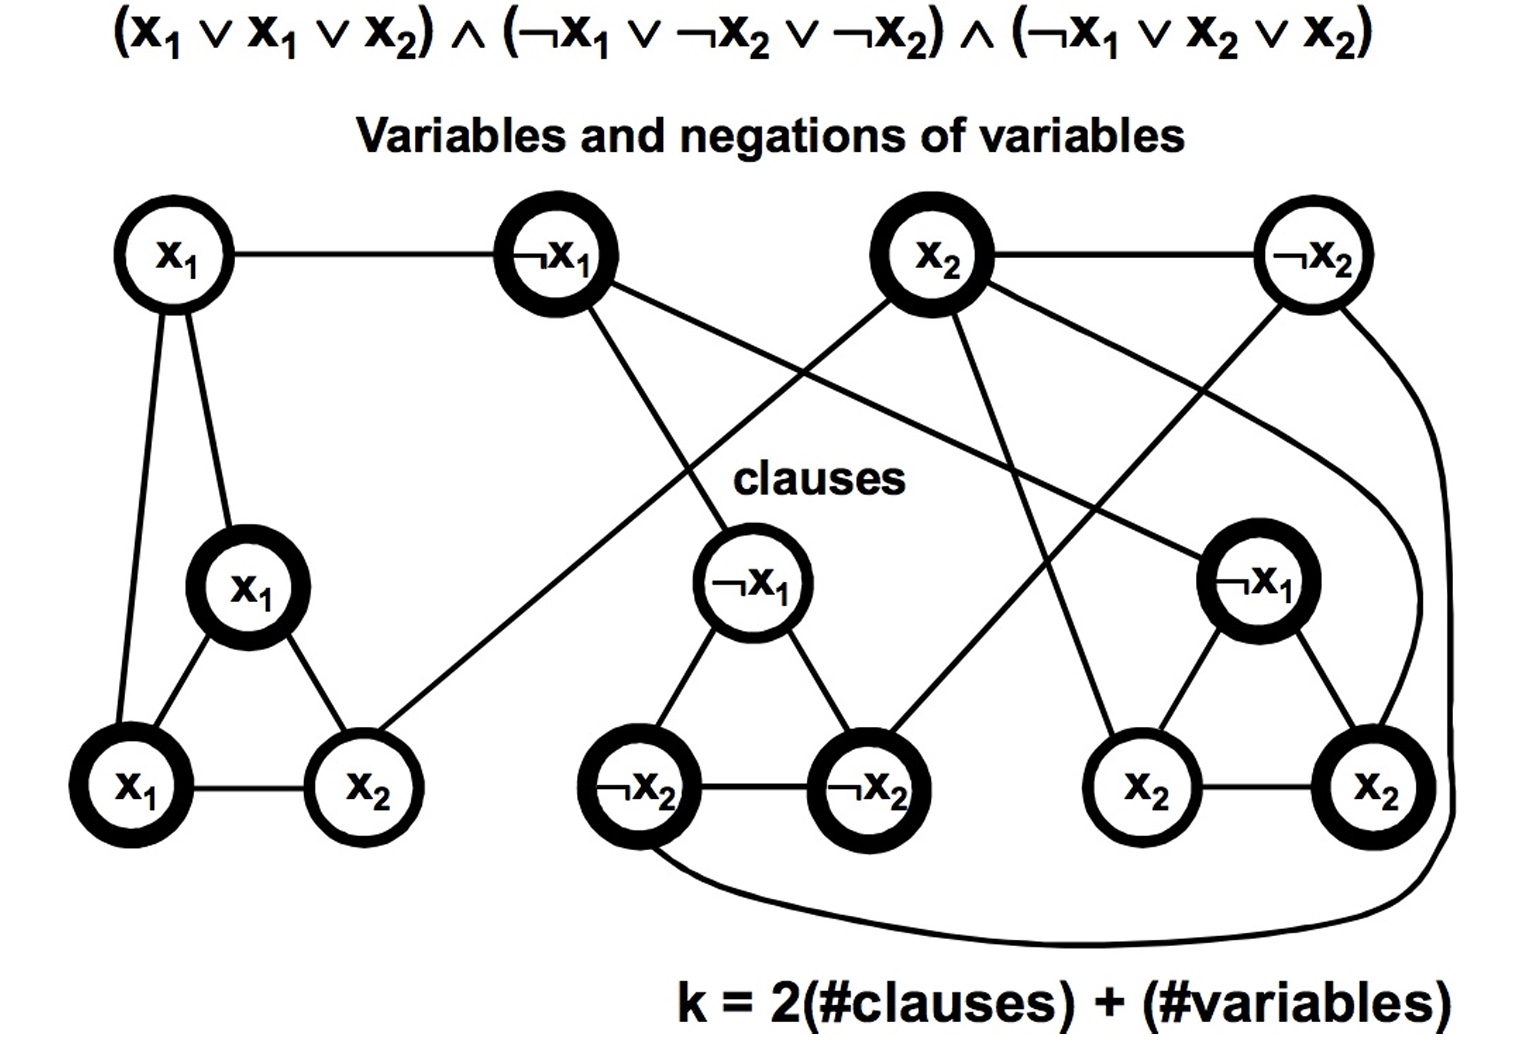
\includegraphics[width=\columnwidth]{3satvc.jpeg}
    \end{figure}
\subsubsection*{Structure of Any Vertex Cover of Size $\le k$}

Observe:
\begin{enumerate}
    \item For each variable pair \((u_i, w_i)\), at least one must be taken in any vertex cover.
    \item For each clause triangle \((z_{j,1}, z_{j,2}, z_{j,3})\), at least two vertices must be taken to cover all three edges.
\end{enumerate}

Thus any vertex cover of size at most \(n + 2m\) must contain:
\[
\text{exactly one of } u_i, w_i \text{ for each } i,
\qquad\text{and}\qquad
\text{exactly two of } z_{j,1}, z_{j,2}, z_{j,3} \text{ for each } j.
\]

\subsubsection*{Satisfying Assignment \(\Rightarrow\) Vertex Cover}

Assume the 3SAT instance is satisfiable.
Let the assignment satisfy every clause.

Construct a vertex cover \(V'\) as follows:
\begin{itemize}
    \item For each variable \(x_i\):
    \[
    u_i \in V' \;\text{iff}\; x_i = \text{true},
    \qquad
    w_i \in V' \;\text{iff}\; x_i = \text{false}.
    \]
    \item For each clause \(c_j\):
    choose two of \(z_{j,1}, z_{j,2}, z_{j,3}\) to include in \(V'\), leaving out
    \(z_{j,r}\) whose corresponding literal \(\ell_{j,r}\) is true.
\end{itemize}

All edges are covered:
\begin{itemize}
    \item variable edges by construction,
    \item clause edges because two vertices of each clause triangle are selected,
    \item literal–variable edges because a literal left out corresponds to a true literal, and its adjacent variable node is in the cover.
\end{itemize}

Hence \(V'\) is a vertex cover of size \(n + 2m = k\).

\subsubsection*{Vertex Cover \(\Rightarrow\) Satisfying Assignment}

Conversely, suppose \(G\) has a vertex cover \(V'\) of size at most \(n + 2m\).
Then:
\[
u_i \in V' \text{ or } w_i \in V' \quad (i = 1,\dots,n),
\]
and exactly two of \(\{z_{j,1},z_{j,2},z_{j,3}\}\) lie in \(V'\) for each clause.

Define the truth assignment:
\[
x_i = \text{true} \iff u_i \in V'.
\]

Consider a clause \(c_j\).  
Let \(z_{j,r}\) be the unique clause vertex \emph{not} included in \(V'\).
Because the edge \((z_{j,r}, s_i)\) must be covered, where
\[
s_i = \begin{cases}
u_i & \text{if } \ell_{j,r} = x_i, \\
w_i & \text{if } \ell_{j,r} = \neg x_i,
\end{cases}
\]
the corresponding \(s_i\) must be in \(V'\).  
Thus \(\ell_{j,r}\) is true under the assignment.
Hence each clause has at least one true literal, and the formula is satisfied.

\subsubsection*{Conclusion}

The above reduction shows that 3SAT \(\le_P\) \textsc{Vertex Cover}, and since
\textsc{Vertex Cover} is in NP, the problem is NP-complete.

\subsection{Reduction from \textsc{Vertex Cover} to \textsc{Hitting Set}}

We show a polynomial-time reduction from \textsc{Vertex Cover} to
\textsc{Hitting Set}.  Intuitively, each edge of the graph becomes a
2-element set that must be ``hit'', and each vertex is an element which can
hit all sets (edges) it is incident to.

\subsubsection*{Problem Definitions}

\paragraph{Vertex Cover.}
An instance of \textsc{Vertex Cover} consists of:
\begin{itemize}
    \item an undirected graph $G = (V,E)$,
    \item an integer $k$.
\end{itemize}
Question: does there exist a subset $C \subseteq V$ with $|C| \le k$ such that
every edge $e = \{u,v\} \in E$ has at least one endpoint in $C$?  Such a set
$C$ is called a \emph{vertex cover}.

\paragraph{Hitting Set.}
An instance of \textsc{Hitting Set} (set hitting) consists of:
\begin{itemize}
    \item a finite universe $U$,
    \item a collection $\mathcal{F}$ of subsets of $U$,
    \item an integer $k$.
\end{itemize}
Question: does there exist a subset $H \subseteq U$ with $|H| \le k$ such that
$H$ intersects every set $F \in \mathcal{F}$ (i.e.\ $H \cap F \ne \emptyset$)?
Such an $H$ is called a \emph{hitting set} (or transversal).

\paragraph{Conceptual Note.}
Vertex Cover can be seen as a special case of Hitting Set:
\begin{itemize}
    \item Vertices $\leftrightarrow$ universe elements.
    \item Edges $\leftrightarrow$ 2-element subsets that must be hit.
    \item A vertex cover $\leftrightarrow$ a hitting set.
\end{itemize}
The reduction just formalizes this observation.

\subsubsection*{Construction}

Let $(G,k)$ be an instance of \textsc{Vertex Cover}, where $G=(V,E)$.

We construct a \textsc{Hitting Set} instance $(U,\mathcal{F},k')$ as follows:

\begin{itemize}
    \item Universe:
    \[
        U := V.
    \]
    That is, each vertex of the graph becomes an element of the universe.

    \item Family of subsets:
    for each edge $e = \{u,v\} \in E$, define a subset
    \[
        F_e := \{u, v\} \subseteq U.
    \]
    Then let
    \[
        \mathcal{F} := \{ F_e : e \in E \}.
    \]

    \item Parameter:
    \[
        k' := k.
    \]
\end{itemize}

This completes the description of the hitting set instance.

\subsubsection*{Correctness of the Reduction}

We prove that $(G,k)$ is a YES-instance of \textsc{Vertex Cover} if and only if
$(U,\mathcal{F},k')$ is a YES-instance of \textsc{Hitting Set}.

\paragraph{($\Rightarrow$) Vertex Cover $\Rightarrow$ Hitting Set.}

Assume there exists a vertex cover $C \subseteq V$ with $|C| \le k$.

For each edge $e = \{u,v\} \in E$, by definition of vertex cover, at least one
of $u$ or $v$ lies in $C$.  Thus:
\[
    C \cap \{u,v\} \ne \emptyset
    \quad\text{for all } e = \{u,v\} \in E.
\]
Equivalently,
\[
    C \cap F_e \ne \emptyset \quad\text{for all } F_e \in \mathcal{F}.
\]
Therefore $C$ is a hitting set of size at most $k' = k$ for the family
$\mathcal{F}$.  Hence $(U,\mathcal{F},k')$ is a YES-instance of
\textsc{Hitting Set}.

\paragraph{($\Leftarrow$) Hitting Set $\Rightarrow$ Vertex Cover.}

Conversely, assume there exists a hitting set $H \subseteq U$ with
$|H| \le k'$ such that $H$ intersects every $F_e \in \mathcal{F}$.

Recall that $U = V$ and each $F_e = \{u,v\}$ for an edge $e=\{u,v\}\in E$.
Since $H$ is a hitting set:
\[
    H \cap F_e \ne \emptyset
    \quad\text{for every } e = \{u,v\} \in E.
\]
That is, for every edge $e = \{u,v\}$, we have $u \in H$ or $v \in H$ (possibly both).

Therefore $H$ is a vertex cover of $G$ and
\[
    |H| \le k' = k.
\]
So $(G,k)$ is a YES-instance of \textsc{Vertex Cover}.

\subsubsection*{Complexity}

The construction is clearly polynomial-time:
\begin{itemize}
    \item We set $U = V$, which just copies the vertex set.
    \item For each edge $e = \{u,v\}$, we create a 2-element subset $F_e$.
\end{itemize}
Thus the size of $(U,\mathcal{F},k')$ is $\mathcal{O}(|V| + |E|)$, and the
conversion can be done in time polynomial in the size of $G$.

\subsubsection*{Conclusion}

We have defined a polynomial-time reduction
\[
    \textsc{Vertex Cover} \le_p \textsc{Hitting Set}.
\]
Since \textsc{Vertex Cover} is NP-complete and \textsc{Hitting Set} is in NP,
it follows that \textsc{Hitting Set} is NP-complete.

\subsection{Reduction from \textsc{Vertex Cover} to \textsc{Set Cover}}

We present a polynomial-time reduction from \textsc{Vertex Cover} to
\textsc{Set Cover}.  Informally, each \emph{vertex} becomes a \emph{set} of
edges it can cover, and each \emph{edge} becomes an \emph{element} that must be
covered by at least one chosen set.

\subsubsection*{Problem Definitions}

\paragraph{Vertex Cover.}
An instance of \textsc{Vertex Cover} consists of:
\begin{itemize}
    \item an undirected graph $G = (V,E)$,
    \item an integer $k$.
\end{itemize}
Question: does there exist a set $C \subseteq V$ with $|C| \le k$ such that
every edge $e = \{u,v\} \in E$ has at least one endpoint in $C$?
Such a set $C$ is called a \emph{vertex cover}.

\paragraph{Set Cover.}
An instance of \textsc{Set Cover} consists of:
\begin{itemize}
    \item a universe $U$ of elements,
    \item a collection of subsets $\mathcal{S} = \{S_1,\dots,S_m\}$ with
          $S_i \subseteq U$,
    \item an integer $k$.
\end{itemize}
Question: does there exist a subcollection
$\mathcal{C} \subseteq \mathcal{S}$ with $|\mathcal{C}| \le k$ such that
\[
    \bigcup_{S \in \mathcal{C}} S = U?
\]
Such a subcollection $\mathcal{C}$ is a \emph{set cover} of size at most $k$.

\paragraph{Conceptual Note.}
There is a natural duality:
\begin{itemize}
    \item \emph{Edges} correspond to \emph{universe elements} that must be covered.
    \item Each \emph{vertex} corresponds to the set of edges incident to it.
    \item A vertex cover is exactly a choice of vertices whose incident-edge
          sets cover all edges.
\end{itemize}
The reduction just encodes this duality formally.

\subsubsection*{Construction}

Given a \textsc{Vertex Cover} instance $(G,k)$ with $G=(V,E)$, we construct a
\textsc{Set Cover} instance $(U,\mathcal{S},k')$ as follows.

\begin{itemize}
    \item \textbf{Universe.}
    Let
    \[
        U := E,
    \]
    so each edge $e \in E$ becomes a universe element.

    \item \textbf{Subsets.}
    For each vertex $v \in V$, define a subset
    \[
        S_v := \{ e \in E : e \text{ is incident to } v \}.
    \]
    Then let
    \[
        \mathcal{S} := \{ S_v : v \in V \}.
    \]
    That is, each vertex gives a set containing exactly the edges it can cover.

    \item \textbf{Parameter.}
    Set
    \[
        k' := k.
    \]
\end{itemize}

This completes the construction of the \textsc{Set Cover} instance.

\subsubsection*{Correctness of the Reduction}

We prove that $(G,k)$ is a YES-instance of \textsc{Vertex Cover} if and only if
$(U,\mathcal{S},k')$ is a YES-instance of \textsc{Set Cover}.

\paragraph{($\Rightarrow$) From Vertex Cover to Set Cover.}

Assume there is a vertex cover $C \subseteq V$ with $|C| \le k$.

Consider the subcollection
\[
    \mathcal{C} := \{ S_v : v \in C \} \subseteq \mathcal{S}.
\]
We claim that $\mathcal{C}$ covers all of $U$.

Let $e \in U$ be any universe element.  Since $U = E$, $e$ is an edge of $G$:
say $e = \{u,w\} \in E$.  Because $C$ is a vertex cover, at least one of
$u,w$ is in $C$.  Suppose $u \in C$.  By construction,
\[
    e \in S_u \in \mathcal{C}.
\]
Thus $e$ belongs to the union $\bigcup_{S \in \mathcal{C}} S$.

Since this holds for every edge $e \in E = U$, we have
\[
    \bigcup_{S \in \mathcal{C}} S = U.
    \quad\text{and}\quad
    |\mathcal{C}| = |C| \le k' = k.
\]
Hence $(U,\mathcal{S},k')$ is a YES-instance of \textsc{Set Cover}.

\paragraph{($\Leftarrow$) From Set Cover to Vertex Cover.}

Conversely, suppose there exists a set cover
$\mathcal{C} \subseteq \mathcal{S}$ with $|\mathcal{C}| \le k'$ such that
\[
    \bigcup_{S \in \mathcal{C}} S = U.
\]

Since $\mathcal{S} = \{S_v : v \in V\}$, each set in $\mathcal{C}$ has the
form $S_v$ for some vertex $v \in V$.  Define
\[
    C := \{ v \in V : S_v \in \mathcal{C} \}.
\]
Then $|C| = |\mathcal{C}| \le k' = k$.

We claim that $C$ is a vertex cover of $G$.

Let $e \in E$ be any edge.  As $U = E$, $e$ is a universe element and must be
covered by $\mathcal{C}$, so there exists some $S_v \in \mathcal{C}$ such that
$e \in S_v$.  By construction of $S_v$, this means that edge $e$ is incident
to vertex $v$.  Since $S_v \in \mathcal{C}$, we have $v \in C$.

Therefore, for every edge $e = \{u,w\}$ in $E$, at least one endpoint belongs
to $C$.  Hence $C$ is a vertex cover of $G$ with size at most $k$.

\subsubsection*{Complexity}

The size of $(U,\mathcal{S},k')$ is polynomial in $|V| + |E|$:
\begin{itemize}
    \item $U$ has one element per edge.
    \item $\mathcal{S}$ has one set per vertex, and each $S_v$ contains all
          edges incident to $v$.
\end{itemize}
Constructing all sets $S_v$ requires scanning each edge once and adding it to
both endpoints’ sets.  Thus the reduction runs in time $\mathcal{O}(|V| + |E|)$.

\subsubsection*{Conclusion}

We have defined a polynomial-time reduction
\[
    \textsc{Vertex Cover} \le_p \textsc{Set Cover}.
\]
Since \textsc{Vertex Cover} is NP-complete and \textsc{Set Cover} is in NP, it
follows that \textsc{Set Cover} is NP-complete.
\subsection{Reduction from \textsc{Set Cover} to \textsc{Dominating Set}}

We present a polynomial-time reduction from \textsc{Set Cover} to
\textsc{Dominating Set}.  The construction is standard: each set becomes a
vertex that dominates the elements it contains.

\subsubsection*{Problem Definitions}

\paragraph{Set Cover.}
An instance of \textsc{Set Cover} consists of:
\begin{itemize}
    \item a universe $U = \{u_1,\dots,u_n\}$,
    \item a family of subsets $\mathcal{S} = \{S_1,\dots,S_m\}$ with
          $S_i \subseteq U$,
    \item an integer $k$.
\end{itemize}
Question: is there a subfamily $\mathcal{C} \subseteq \mathcal{S}$ with
$|\mathcal{C}| \le k$ such that $\bigcup_{S \in \mathcal{C}} S = U$?

\paragraph{Dominating Set.}
Given a graph $G=(V,E)$ and an integer $k$, the question is whether there is a
subset $D \subseteq V$ with $|D| \le k$ such that every vertex $v \in V$ is
either in $D$ or adjacent to some vertex in $D$.  Such a $D$ is a
\emph{dominating set}.

\paragraph{Conceptual Note.}
Interpretation:
\begin{itemize}
    \item each set $S_i$ will be a vertex that “dominates” the elements in $S_i$,
    \item picking a vertex in the dominating set corresponds to choosing the set,
    \item ensuring every element vertex is dominated corresponds to covering all
          universe elements.
\end{itemize}

\subsubsection*{Construction}

Given a set cover instance $(U,\mathcal{S},k)$, we construct a graph
$G = (V,E)$ and integer $k'$ as follows.

\paragraph{Vertices.}
Create two types of vertices:
\[
    V = V_{\text{set}} \,\cup\, V_{\text{elem}},
\]
where
\begin{itemize}
    \item for each set $S_i \in \mathcal{S}$, create a vertex $s_i \in V_{\text{set}}$,
    \item for each element $u_j \in U$, create a vertex $e_j \in V_{\text{elem}}$.
\end{itemize}

\paragraph{Edges.}
Add edges according to set membership:
\[
    (s_i, e_j) \in E \quad\Longleftrightarrow\quad u_j \in S_i.
\]

Finally, make all set-vertices adjacent to each other (a clique):
\[
    \forall i \ne i',\quad (s_i, s_{i'}) \in E.
\]

\paragraph{Parameter.}
Let
\[
    k' := k.
\]

\subsubsection*{Intuition Behind the Gadget}

\begin{itemize}
    \item Each $e_j$ (element vertex) must be dominated, so at least one
          $s_i$ with $u_j \in S_i$ must be chosen.
    \item Making the $s_i$ all adjacent ensures:
        \begin{itemize}
            \item If we pick any $s_i$, \emph{all} $s$-vertices are automatically dominated.
            \item There is never a need to include element vertices $e_j$ in
                  the dominating set (this would waste budget).
        \end{itemize}
    \item Thus a minimum dominating set will consist only of $s_i$-vertices,
          which correspond exactly to sets chosen in the cover.
\end{itemize}

\subsubsection*{Correctness}

\paragraph{($\Rightarrow$) From Set Cover to Dominating Set.}

Suppose $\mathcal{C} \subseteq \mathcal{S}$ is a set cover with $|\mathcal{C}| \le k$.
Let
\[
    D := \{\, s_i : S_i \in \mathcal{C} \,\}.
\]
Then $|D| = |\mathcal{C}| \le k' = k$.

We show $D$ is a dominating set:

\begin{itemize}
    \item Every set-vertex $s_i$ is adjacent to every vertex in $D$ since
          $V_{\text{set}}$ is a clique.
    \item Every element-vertex $e_j$ corresponds to an element $u_j \in U$, and
          since $\mathcal{C}$ is a set cover, there exists $S_i \in \mathcal{C}$
          such that $u_j \in S_i$.  Hence $e_j$ is adjacent to $s_i \in D$.
\end{itemize}

Thus all vertices are dominated by $D$, so $(G,k')$ is a YES-instance of
\textsc{Dominating Set}.

\paragraph{($\Leftarrow$) From Dominating Set to Set Cover.}

Conversely, suppose $D \subseteq V$ is a dominating set with $|D| \le k'$.

\begin{itemize}
    \item If $D$ contains an element-vertex $e_j$, we can replace it by any
          adjacent set-vertex (there is always at least one, since $e_j$ must be
          dominated).  This never increases the size of $D$.
    \item Repeating this for all such $e_j$ yields a dominating set $D'$ of size
          $\le k'$ containing \emph{only} set-vertices.
\end{itemize}

Let
\[
    \mathcal{C} := \{\, S_i : s_i \in D' \,\}.
\]

Every element $u_j \in U$ must be dominated by some $s_i \in D'$, and the edge
$(s_i, e_j)$ exists only if $u_j \in S_i$.  Therefore every $u_j$ is contained
in at least one set $S_i \in \mathcal{C}$, proving that $\mathcal{C}$ is a set
cover with $|\mathcal{C}| \le k$.

\subsubsection*{Complexity}

The construction uses $|V| = m + n$ vertices and $|E| =
\sum_{i=1}^m |S_i| + \binom{m}{2}$ edges, which is polynomial in the input size.
Therefore the reduction runs in polynomial time.

\subsubsection*{Conclusion}

This construction gives a polynomial-time reduction
\[
    \textsc{Set Cover} \le_p \textsc{Dominating Set}.
\]
Hence, since \textsc{Set Cover} is NP-complete and \textsc{Dominating Set} is in NP,
\textsc{Dominating Set} is NP-complete.


\subsection{WA3 Task 2: Complexity of MIS Variants}

In this task we investigate the computational complexity of several variants of 
the maximal independent set (MIS) problem.  
We assume familiarity with the definitions of maximal independent set, 
Extend-MIS-out (from WA2), and vertex cover (from lectures).  
We study the following decision problems:

\paragraph{min-MIS.}
\begin{itemize}
    \item \textbf{Input:} A simple undirected graph $G=(V,E)$ and an integer $k\ge 0$.
    \item \textbf{Question:} Does $G$ have a maximal independent set $S\subseteq V$ with $|S|\le k$?
\end{itemize}

\paragraph{min-VC.}
\begin{itemize}
    \item \textbf{Input:} A simple undirected graph $G=(V,E)$ and an integer $k\ge 0$.
    \item \textbf{Question:} Does $G$ have a vertex cover $C\subseteq V$ with $|C|\le k$?
\end{itemize}

%---------------------------------------------
\subsubsection*{1.\quad Extend-MIS-out is in NP}

A certificate is a maximal independent set $I\subseteq V$ such that $S\cap I=\emptyset$.
Verification consists of:

\begin{itemize}
    \item \textbf{Independence:} For each edge $\{u,v\}\in E$, ensure that $\{u,v\}\nsubseteq I$.
    \item \textbf{Maximality:} For each $v\in V\setminus I$, check that $v$ has a neighbor in $I$.
\end{itemize}

Both checks take $O(|E|)$ time using adjacency lists.  
Hence, Extend-MIS-out $\in \text{NP}$.

%---------------------------------------------
\subsubsection*{2.\quad Extend-MIS-out is NP-complete (reduction from 3-SAT)}

Given a 3-SAT instance $\varphi$, construct $(G,S)$ as follows:

\begin{enumerate}
    \item For each literal $\ell$, create a vertex $v_\ell$.
    \item For each variable $x$, create a vertex $s_x$ and make  
          $\{s_x, v_x, v_{\neg x}\}$ a 3-clique.  
          Add $s_x$ to $S$.  
          This enforces exactly one of $v_x$ or $v_{\neg x}$ to appear in the MIS.
    \item For each clause $C=(\ell_1\lor\ell_2\lor\ell_3)$, create a vertex $s_C$  
          adjacent to $v_{\ell_1}$, $v_{\ell_2}$, $v_{\ell_3}$, and add $s_C$ to $S$.  
          This forces at least one literal of each clause to be chosen in any MIS disjoint from $S$.
\end{enumerate}

\paragraph{Correctness.}

\textbf{If $\varphi$ is satisfiable:}  
Let $I$ contain exactly the vertices $v_\ell$ corresponding to true literals.  
This set is independent and maximal, and is disjoint from $S$.

\textbf{If $(G,S)$ is a YES-instance:}  
Any maximal independent set $I$ with $I\cap S=\emptyset$ must contain exactly one of  
$\{v_x, v_{\neg x}\}$ for each variable, defining a truth assignment.  
Each clause vertex $s_C\in S$ enforces that at least one of its three literals is in $I$,  
so the assignment satisfies $\varphi$.

Thus Extend-MIS-out is NP-complete.


%---------------------------------------------
\subsubsection*{3.\quad min-MIS is in NP}

A certificate is a maximal independent set $S\subseteq V$ with $|S|\le k$.  
We verify:

\begin{itemize}
    \item $S$ is independent (scan edges),
    \item $S$ is maximal (every $v\notin S$ has a neighbor in $S$),
    \item $|S|\le k$.
\end{itemize}

All checks take polynomial time, so min-MIS $\in\text{NP}$.


%---------------------------------------------
\subsubsection*{4.\quad The naive reduction from min-VC to min-MIS does not work}

Proposed mapping:
\begin{itemize}
    \item For each edge $e=\{u,v\}$ in $G$, introduce a new vertex $s_e$ and replace $e$ with the path
          $u - s_e - v$.
    \item Set $k'=k$.
\end{itemize}

Counterexample:  
Let $G$ be a 3-vertex path.  
Then $(G,k=1)$ is a YES-instance of min-VC (choose the middle vertex).  
But the transformed graph $G'$ becomes a 5-vertex path, in which every maximal independent set has size at least $2$.  
Hence $(G',1)$ is a NO-instance of min-MIS.  
Thus this reduction fails.


%---------------------------------------------
\subsubsection*{5.\quad Correct reduction: min-VC $\le_P$ min-MIS}

Let $G=(V,E)$ and $k$ be a min-VC instance.  
Define $k' = |V| + k$ and construct $G'$:

\begin{enumerate}
    \item For each edge $e=\{u,v\}$, replace it with $k'+1$ internally vertex-disjoint paths  
          of length $2$ between $u$ and $v$.
    \item For each vertex $v\in V$, add a new path $(v, v', v'')$.
\end{enumerate}

\paragraph{Correctness.}

\textbf{($\Rightarrow$)}  
Given a vertex cover $C$ of size $\le k$, construct a maximal independent set:
\[
I := \{v, v'': v\in C\} \;\cup\; \{v': v\notin C\}.
\]
Then $|I| = |V| + |C| \le k'$, and $I$ is maximal and independent.

\textbf{($\Leftarrow$)}  
Let $I$ be an MIS of $G'$ with $|I|\le k'=|V|+k$.  
For every $v\in V$, $I$ intersects $\{v,v',v''\}$ in exactly either:
\[
\{v'\} \quad \text{or} \quad \{v, v''\}.
\]
Define $C := \{v : v\in I\}$. Then $|C| = |I|-|V| \le k$.  
Maximality of $I$ guarantees $C$ is a vertex cover.

Thus min-VC $\le_P$ min-MIS, and min-MIS is NP-complete.

\subsection{More Reductions Overview and Examples}
\begin{enumerate}
    \item 3SAT $\le_P$ Vertex 3-Coloring,
    \item 3SAT $\le_P$ Hamiltonian Cycle,
    \item 3SAT $\le_P$ Super Mario (game NP-hardness framework).
\end{enumerate}
Each reduction is based on constructing \emph{gadgets} that encode the logical
structure of a 3SAT formula inside the constraints of the target problem.

\subsubsection{Polynomial-Time Reductions}
A polynomial-time (Karp) reduction from problem $A$ to problem $B$ is an algorithm
that maps any instance of $A$ to an instance of $B$, in polynomial time, such that
the two instances have the same answer. Formally,
\[
A \le_P B \quad\Longleftrightarrow\quad
\text{there exists polytime } f \text{ such that }
x \in A \iff f(x) \in B.
\]
This implies that $B$ is \emph{at least as hard} as $A$: a polynomial-time algorithm
for $B$ immediately yields one for $A$. To prove NP-hardness, we typically reduce
from a known NP-complete problem such as 3SAT using small, local \emph{gadgets}
that simulate variables, clauses, or logical constraints.

\subsubsection{Reduction: 3SAT to Vertex 3-Coloring}
Given a 3SAT instance, the goal is to construct a graph that is 3-colorable iff
the formula is satisfiable. The reduction uses clause gadgets that force the
vertices corresponding to literals in a clause to be assigned colors that encode
whether the literals can be simultaneously satisfied.  
The construction guarantees:
\begin{itemize}
    \item If the formula is satisfiable, a consistent 3-coloring exists.
    \item If the formula is unsatisfiable, no proper 3-coloring exists.
\end{itemize}
Thus Vertex 3-Coloring is NP-hard, and because it is also in NP, it is NP-complete.

\subsubsection{Reduction: 3SAT to Hamiltonian Cycle}
To reduce 3SAT to Hamiltonian Cycle, we construct a directed graph in which a
Hamiltonian cycle exists iff the formula is satisfiable. The graph uses:
\begin{itemize}
    \item \textbf{Variable gadgets:} long chains that can be traversed in one
          of two directions, representing TRUE or FALSE assignments.
    \item \textbf{Clause gadgets:} nodes that can be visited only if at least
          one literal in the clause is satisfied.
\end{itemize}
A Hamiltonian cycle must visit all clause gadgets, forcing the traversal to
correspond to a satisfying assignment.  
Conversely, if no satisfying assignment exists, at least one clause gadget is
inaccessible, preventing a Hamiltonian cycle from existing.

\subsubsection{Reduction: 3SAT to Super Mario}
The NP-hardness of Super Mario (and many other platform games) is established
via a general framework that reduces 3SAT to in-game progression puzzles.
The reduction makes use of several carefully designed \emph{gameplay gadgets}:
\begin{itemize}
    \item \textbf{Start \& Finish gadgets:}
          enforce an initial and final configuration (e.g., Mario must be large).
    \item \textbf{Variable gadgets:}
          force the player to commit to a TRUE or FALSE choice, and prevent
          switching afterwards.
    \item \textbf{Clause gadgets:}
          can be ``unlocked'' by visiting through at least one literal path.
    \item \textbf{Check path:}
          ensures that the player can reach the goal only if \emph{all} clauses
          have been unlocked.
    \item \textbf{Crossover gadgets:}
          allow literal paths to cross without permitting leakage between them.
\end{itemize}
The player completes the level iff all clauses are satisfied, establishing
NP-hardness of the game.

\subsubsection{Takeaways}
Across all three reductions, a unifying theme emerges:
\begin{itemize}
    \item Logical constraints in 3SAT are encoded using small gadgets.
    \item The constructed instance in the target problem mirrors the structure
          of the Boolean formula.
    \item The correctness direction always proceeds by showing:
          \[
          \text{Satisfying assignment} \iff \text{Valid solution in the target problem.}
          \]
\end{itemize}
These reductions demonstrate the versatility of gadget constructions and the
central role of 3SAT in NP-hardness proofs.
\subsection{3-Partition $\leq_P$ 2-partition(partition)}
\subsection{Partition $\leq_P$ 0/1 Knapsack}
\subsubsection*{Problem definition} 
\subsubsection*{Partition}
Given a multiset $S$, whether there exists a partition of $S$, $S_1$ and $S_2$, such that $\sum S_1 = \sum S_2 = \frac{1}{2} \sum S$
\subsubsection*{0/1 Knapsack}
Given a multiset of $n$ items $I = \{(w_i, v_i) | i \in [1,n]\}$, and a weight limit $W$, 
\[\text{maximize } \sum_{i=1}^{n} x_iv_i, \quad\text{such that } \sum_{i=1}^{n}x_iw_i \leq W\]
for the decision version, for a target value $k$, whether there exists a selection such that 
\[\sum_{i=1}^{n} x_iv_i \geq k, \quad\text{while } \sum_{i=1}^{n}x_iw_i \leq W\]
\subsubsection*{Construction} 
Given an instance of partition $(S)$ of size $n$, let $m = \sum S$, the target partiton sum is $m/2$, consider the following construction of a 0/1 knapsack instance:
\[I = \{(\frac{S[i]}{2}, \frac{S[i]}{2}) | i \in [1,n]\}, \quad{W = m}, \quad k = m\]
\subsubsection*{Partiton(YES) $\leq_P$ Knapsack(YES)}

\subsubsection*{Knapsack(YES) $\leq_P$ Partition(YES)}
\subsection{0/1 Knapsack $\leq_P$ coin change}
\subsubsection*{Problem definition} 
\subsubsection*{0/1 Knapsack}
\[\]
\end{document}
